% -*- TeX-master: "sbml-level-3-version-1-core"; fill-column: 66 -*-
% ----------------------------------------------------------------
% Description       : Top-level file for SBML L2V3R1 specification
% Original author(s): Michael Hucka <mhucka@caltech.edu>
% Organization      : California Institute of Technology
% $Id$
% $HeadURL$
% ----------------------------------------------------------------

\documentclass{sbmlspec}

% Emacs: -*- TeX-master: "sbml-level-3-version-2-core"; fill-column: 66 -*-
% -----------------------------------------------------------------------------
% Description       : Version/level-specific LaTeX definitions & helpers
% Original author(s): Michael Hucka <mhucka@caltech.edu>
% Organization      : California Institute of Technology
% -----------------------------------------------------------------------------

% Which level/version/release is this?

\newcommand{\sbmllevel}    {3}
\newcommand{\sbmlversion}  {\changed{2} Core}
\newcommand{\sbmlversionNC}{2 Core}
\newcommand{\sbmlversionnum}{\changed{2}}
\newcommand{\sbmlrelease}  {1 \changed{(Draft)}}
\newcommand{\sbmlreleaseNC}{1 (Draft)}
\newcommand{\sbmldate}     {\changed{XX December 2015}}

\newcommand{\thisRelease}  {Release~\sbmlrelease{}\xspace}
\newcommand{\thisL}	   {Level~\sbmllevel\xspace}
\newcommand{\thisV}	   {\changed{Version}~\sbmlversion}
\newcommand{\thisVnum}	   {\changed{Version}~\sbmlversionnum\xspace}
\newcommand{\thisLV}       {Level~\sbmllevel{} \thisV\xspace}
\newcommand{\thisLVNC}     {Level~\sbmllevel{} Version~\sbmlversionNC\xspace}
\newcommand{\thisLVnum}    {Level~\sbmllevel{} \thisVnum}
\newcommand{\thisLVR}      {\thisLV \thisRelease}

\newcommand{\previousLVR}  {Level~3 Version~1 Release~1}

% Special commands for web addresses:

\newcommand{\sbmlSchemasURL}{\url{http://sbml.org/specifications/sbml-level-\sbmllevel/version-2/schemas/}}

% Special commands for linking the SBML component classes in this document.
% The following defines a special command of the form \Foo for any SBML
% type that has a UML box in the spec.  Note that SId is not in this
% list -- it doesn't have a UML class definition.

\newcommand{\AlgebraicRule}{\defRef{AlgebraicRule}{sec:algebraicrule}}
\newcommand{\Annotation}{\defRef{Annotation}{sec:sbase}}
\newcommand{\AssignmentRule}{\defRef{AssignmentRule}{sec:assignmentrule}}
\newcommand{\Compartment}{\defRef{Compartment}{sec:compartments}}
\newcommand{\Constraint}{\defRef{Constraint}{sec:constraints}}
\newcommand{\Delay}{\defRef{Delay}{sec:event-delay}}
\newcommand{\EventAssignment}{\defRef{EventAssignment}{sec:eventassignment}}
\newcommand{\Event}{\defRef{Event}{sec:events}}
\newcommand{\Events}{\defRef{Events}{sec:events}}
\newcommand{\FunctionDefinition}{\defRef{FunctionDefinition}{sec:functiondefinition}}
\newcommand{\InitialAssignment}{\defRef{InitialAssignment}{sec:initialAssignment}}
\newcommand{\KineticLaw}{\defRef{KineticLaw}{subsec:kinetic-law}}
\newcommand{\ListOfCompartments}{\defRef{ListOfCompartments}{sec:listofcompartments}}
\newcommand{\ListOfConstraints}{\defRef{ListOfConstraints}{sec:listofconstraints}}
\newcommand{\ListOfEventAssignments}{\defRef{ListOfEventAssignments}{sec:listofeventassignments}}
\newcommand{\ListOfEvents}{\defRef{ListOfEvents}{sec:listofevents}}
\newcommand{\ListOfFunctionDefinitions}{\defRef{ListOfFunctionDefinitions}{sec:listoffunctiondefinitions}}
\newcommand{\ListOfInitialAssignments}{\defRef{ListOfInitialAssignments}{sec:listofinitialassign}}
\newcommand{\ListOfLocalParameters}{\defRef{ListOfLocalParameters}{subsec:listoflocalparameters}}
\newcommand{\ListOfModifierSpeciesReferences}{\defRef{ListOfModifierSpeciesReferences}{sec:reaction-type}}
\newcommand{\ListOfPackages}{\defRef{ListOfPackages}{sec:listofpackages}}
\newcommand{\ListOfParameters}{\defRef{ListOfParameters}{sec:listofparameters}}
\newcommand{\ListOfReactions}{\defRef{ListOfReactions}{sec:listofreactions}}
\newcommand{\ListOfRules}{\defRef{ListOfRules}{sec:listofrules}}
\newcommand{\ListOfSpeciesReferences}{\defRef{ListOfSpeciesReferences}{sec:reaction-type}}
\newcommand{\ListOfSpecies}{\defRef{ListOfSpecies}{sec:listofspecies}}
\newcommand{\ListOfUnitDefinitions}{\defRef{ListOfUnitDefinitions}{sec:listofunitdefinitions}}
\newcommand{\ListOfUnits}{\defRef{ListOfUnits}{sec:listofunits}}
\newcommand{\ListOf}{\class{ListOf\rule{0.3in}{0.5pt}}\xspace}
\newcommand{\LocalParameter}{\defRef{LocalParameter}{subsec:localparameter}}
\newcommand{\LocalParameters}{\defRef{LocalParameters}{subsec:localparameter}}
\newcommand{\Message}{\defRef{Message}{sec:constraints}}
\newcommand{\Model}{\defRef{Model}{sec:model}}
\newcommand{\ModifierSpeciesReference}{\defRef{ModifierSpeciesReference}{sec:simplespeciesreference-sboterm}}
\newcommand{\Notes}{\defRef{Notes}{sec:sbase}}
\newcommand{\Package}{\defRef{Package}{sec:package}}
\newcommand{\Parameter}{\defRef{Parameter}{sec:parameters}}
\newcommand{\Priority}{\defRef{Priority}{sec:event-priority}}
\newcommand{\RateRule}{\defRef{RateRule}{sec:raterule}}
\newcommand{\Reaction}{\defRef{Reaction}{sec:reactions}}
\newcommand{\RuleUpright}{\absDefRefUpright{Rule}{sec:rules}}
\newcommand{\Rule}{\absDefRef{Rule}{sec:rules}}
\newcommand{\SBML}{\defRef{SBML}{sec:sbml}}
\newcommand{\SBaseUpright}{\absDefRefUpright{SBase}{sec:sbase}}
\newcommand{\SBase}{\absDefRef{SBase}{sec:sbase}}
\newcommand{\SimpleSpeciesReferenceUpright}{\absDefRefUpright{SimpleSpeciesReference}{sec:simplespeciesreference-sboterm}}
\newcommand{\SimpleSpeciesReference}{\absDefRef{SimpleSpeciesReference}{sec:simplespeciesreference-sboterm}}
\newcommand{\SpeciesReference}{\defRef{SpeciesReference}{sec:simplespeciesreference-sboterm}}
\newcommand{\Species}{\defRef{Species}{sec:species}}
\newcommand{\StoichiometryMath}{\defRef{StoichiometryMath}{sec:reactions}}
\newcommand{\Trigger}{\defRef{Trigger}{sec:trigger}}
\newcommand{\UnitDefinition}{\defRef{UnitDefinition}{sec:unitdefinitions}}
\newcommand{\Unit}{\defRef{Unit}{sec:unitdefinitions}}

% Classes without a single section, or which are from other specifications:
\newcommand{\Math}        {\class{Math}\xspace}
\newcommand{\Port}        {\class{Port}\xspace}

% Macros for SBO.

\newcommand{\sboref}{\uri{http://biomodels.net/sbo/}\xspace}

\newcommand{\sboparticipantroleID}{\token{SBO:0000003}}
\newcommand{\sboparticipantrole}{\sboparticipantroleID, ``participant role''\xspace}
\newcommand{\sboeventID}{\token{SBO:0000231}}
\newcommand{\sboevent}{\sboeventID, ``event''\xspace}
\newcommand{\sboproductID}{\token{SBO:0000011}}
\newcommand{\sboproduct}{\sboproductID, ``product''\xspace}
\newcommand{\sboreactantID}{\token{SBO:0000010}}
\newcommand{\sboreactant}{\sboreactantID, ``reactant''\xspace}
\newcommand{\sbomodifierID}{\token{SBO:0000019}}
\newcommand{\sbomodifier}{\sbomodifierID, ``modifier''\xspace}
\newcommand{\sboparameterID}{\token{SBO:0000002}}
\newcommand{\sboparameter}{\sboparameterID, ``quantitative \changed{systems description} parameter''\xspace}
\newcommand{\sboratelawID}{\token{SBO:0000001}}
\newcommand{\sboratelaw}{\sboratelawID, ``rate law''\xspace}
\newcommand{\sbomathformulaID}{\token{SBO:0000064}}
\newcommand{\sbomathformula}{\sbomathformulaID, ``mathematical expression''\xspace}
\newcommand{\sboframeworkID}{\token{SBO:0000004}}
\newcommand{\sboframework}{\sboframeworkID, ``modeling framework''\xspace}
\newcommand{\sbomaterialentityID}{\token{SBO:0000240}}
\newcommand{\sbomaterialentity}{\sbomaterialentityID, ``material entity''\xspace}
\newcommand{\sbointeractionID}{\token{SBO:0000231}}
\newcommand{\sbointeraction}{\sbointeractionID, ``interaction''\xspace}

% Special commands for example models.
% NOTICE THE BLANK LINE.  Make sure to leave it!  Otherwise the
% first line of the inputted file gets indented.

\newcommand{\sbmlexample}[1]{\begin{example}

\vspace*{-0.5ex}
\input{examples/#1}\end{example}}
  % Things that often change with each release.

% ----------------------------------------------------------------
\begin{document}
% ----------------------------------------------------------------

% Front matter:

% -*- TeX-master: "sbml-level-3-version-2-core"; fill-column: 66 -*-
% ----------------------------------------------------------------

\title{{\scalefont{1.1}The Systems Biology Markup Language (SBML):}\\
Language Specification for \thisLV}

\author{\begin{tabular}{l>{\hspace*{15pt}}r}
Michael Hucka (Chair)	& \emph{California Institute of Technology, US}\\
Frank T. Bergmann  	& \emph{California Institute of Technology, US}\\
Claudine Chaouiya  	& \emph{Instituto Gulbenkian de Ci{\^e}ncia, PT}\\
Andreas Dr{\"a}ger  	& \emph{University of T{\"u}bingen, DE}\\
Stefan Hoops		& \emph{Virginia Bioinformatics Institute, US}\\
Sarah M. Keating	& \emph{European Bioinformatics Institute, GB}\\
Matthias K{\"o}nig      & \emph{Humboldt University Berlin, Germany}\\
Nicolas Le~Nov\`{e}re	& \emph{Babraham Institute, GB}\\
Chris J. Myers		& \emph{University of Utah, US}\\
Brett G. Olivier	& \emph{VU University Amsterdam, NL}\\
Sven Sahle		& \emph{University of Heidelberg, DE}\\
James C. Schaff		& \emph{University of Connecticut, US}\\
Rahuman Sheriff		& \emph{European Bioinformatics Institute, GB}\\
Lucian P. Smith		& \emph{University of Washington, US}\\
Dagmar Waltemath	& \emph{University of Rostock, DE}\\
Darren J. Wilkinson	& \emph{Newcastle University, GB}\\
Fengkai Zhang	        & \emph{National Institute of Health, US}\\[8pt]
\end{tabular}\\
\href{mailto:sbml-editors@sbml.org}{\sffamily sbml-editors@sbml.org}}

\date{\vfill \textbf{SBML \thisLV} \\[10pt]
  \textbf{Release \sbmlrelease} \\[10pt]
  \sbmldate}

% Extra settings for the PDF version:

\hypersetup{
 pdftitle={Systems Biology Markup Language (SBML) Level \sbmllevel Core},
 pdfauthor={Michael Hucka, Frank Bergmann, Stefan Hoops, Sarah M. Keating, 
   Nicolas Le~Nov\`{e}re, Chris J. Myers, Brett G. Olivier, Sven Sahle,
   James C. Schaff, Lucian P. Smith, Dagmar Waltemath, and Darren J. Wilkinson},
 pdfsubject={SBML \thisLVR}
}

\maketitle

\vfill

\begin{center}\sffamily
Corrections and other changes to this SBML language specification may appear over time.\\
Notifications of new releases are broadcast on the mailing list \href{http://www.sbml.org/Forums/sbml-announce}{sbml.org/forums/sbml-announce}\\[10pt]

The latest release of the SBML \thisLV specification is available at\\
\url{http://sbml.org/specifications/sbml-level-\sbmllevel/version-\sbmlversionnum/core}\\[10pt]

\emph{This} release of the specification is available at\\
\url{http://sbml.org/specifications/sbml-level-\sbmllevel/version-\sbmlversionnum/core/release-\sbmlreleaseNC/}\\[10pt]

The list of known issues in all releases of SBML \thisLV is available at\\
\url{http://sbml.org/specifications/sbml-level-\sbmllevel/version-\sbmlversionnum/core/errata/}\\[10pt]

Formal schemas for use with XML are available at\\
\sbmlSchemasURL\\[10pt]
\end{center}

\vfill

\centerline{\includegraphics[width=2.5in]{\SBMLLogo}}

\clearpage
\sbmltableofcontents
\clearpage

% Body:

\color{black}   % PDF page coloring is buggy.  Set it straight.
\linenumbers

% -*- TeX-master: "multi" -*-

%%%%%%%%%%%%%%
% introduction
%%%%%%%%%%%%%%
\section{Introduction}
\label{def:Introduction}

This Multistate, Multicomponent and Multicompartment Species (Multi) package provides an extension of \SbmlLevelThreeWC\ that supports encoding \smodels\ with molecular complexes that have multiple components and can exist in multiple states and in multiple \compartments. One of its \mBlockChangedBegin{\revTwentyTwentyMarch}goals is\mBlockChangedEnd{\revTwentyTwentyMarch} to provide a platform for sharing \smodels\ based on the specifications of \mBlockChangedBegin{\revTwentyTwentyMarch} molecular transformations/interactions and the rules governing such reactions\mBlockChangedEnd{\revTwentyTwentyMarch} [\cite{ref:simmune2012, ref:scienceSignaling2006, ref:FeretPnas2009, ref:modeler2013}]. This specification covers the goals and features described in \multiOneProposalWC\ for extending SBML to carry the information for \textit{multistate multicomponent} \species\ with revised data structure. In addition, this specification includes the feature for \textit{multicompartment} \species\ as described in the releases of the Multi proposal [\cite{ref:multiproposal280}, \cite{ref:revisedMulti}].

\subsection{Proposal and specifications}
\label{def:Proposal}

The proposal corresponding to this package specification is available at:

\hspace{3ex}\url{http://sbml.org/Community/Wiki/SBML_Level_3_Proposals/Multistate_and_Multicomponent_Species_Proposal}

The specifications (v1.0.1 to current) are located at: 

\hspace{3ex}\url{https://sourceforge.net/p/sbml/code/HEAD/tree/trunk/specifications/sbml-level-3/version-1/multi/spec/}

\subsection{Package dependencies}
\label{def:Package_dependencies}

The Multi package has no dependencies on other \SbmlLevelThree\ packages.

\subsection{Document conventions}
\label{def:Document_conventions}

UML 1.0 notation is used in this document to define the constructs provided by this package. Colors 
in the diagrams carry the following additional information for the benefit of those viewing the 
document on media that can display color:

\begin{itemize}
 \item {\color{black}\framebox{\textit{Black}}} Items colored black are components taken unchanged 
      from their definitions in the \SbmlLevelThreeCore\ specification document.
 \item {\color{mediumgreen}\dbox{\textit{Green}}} Items colored green are components that exist in 
      \SbmlLevelThreeCore, but are extended by this package. Class boxes are also drawn with with 
      dashed lines to further distinguish them.
 \item {\color{sbmlblue}\framebox{Blue}} Items colored blue are new components introduced in this 
      package specification. They have no equivalent in  the \SbmlLevelThreeCore\ specification. 
\end{itemize}
 
For other matters involving the use of UML, XML and typographical conventions, this document follows the conventions
used in the \SbmlLevelThreeCore\ specification document [\cite{ref:sbmll3v1}].

For simplicity, \val{...} in all example code refers to some unspecified code content, that is not important for the purpose of illustrating the issue at hand.

% -*- TeX-master: "sbml-level-3-version-1-core"; fill-column: 66 -*-
% $Id$
% $HeadURL$
% ----------------------------------------------------------------

\section{Overview of SBML}
\label{sec:overview}

The following is an example of a simple network of
biochemical reactions that can be represented in SBML:
\begin{linenomath}
  \begin{equation*}
    \begin{array}{@{}ccl@{}}
      S_1 & \overset{\underrightarrow{k_1 [S_1] / ([S_1] + k_2)}}{} & S_2 \\ \\[-5pt]
      S_2 & \overset{\underrightarrow{\rule{0.26in}{0pt}k_3 [S_2]\rule{0.26in}{0pt}}}{} & S_3 + S_4
    \end{array}
  \end{equation*}
\end{linenomath}
In this particular set of chemical equations above, the symbols in
square brackets (e.g., ``$[S_1]$'') represent concentrations of molecular
species, the arrows represent reactions, and the formulas above
the arrows represent the rates at which the reactions take place.
(And while this example uses concentrations, it could equally have used
other measures such as molecular counts.)
Broken down into its constituents, this model contains a number of
components: reactant species, product species, reactions,
reaction rates, and parameters in the rate expressions.  To analyze or
simulate this network, additional components must be made
explicit, including compartments for the species, and units on the
various quantities.

SBML allows models of arbitrary complexity to be represented.
Each type of component in a model is described using a specific
type of data object that organizes the relevant information.
The top level of an SBML model definition consists of lists of
these components, with every list being optional:

\vspace*{2ex}
\begin{center}
  \begin{edtable}{tabular}{>{\hspace*{10pt}\slshape}l>{\hspace*{40pt}}l}
    \hspace*{-10pt}beginning of model definition \\
    list of function definitions (optional)	& (Section~\ref{sec:functiondefinition}) \\
    list of unit definitions (optional)	& (Section~\ref{sec:unitdefinitions}) \\
    list of compartments (optional)	 	& (Section~\ref{sec:compartments}) \\
    list of species (optional)		& (Section~\ref{sec:species}) \\
    list of parameters (optional)		& (Section~\ref{sec:parameters}) \\
    list of initial assignments (optional)	& (Section~\ref{sec:initialAssignment}) \\
    list of rules (optional)			& (Section~\ref{sec:rules}) \\
    list of constraints (optional)		& (Section~\ref{sec:constraints}) \\
    list of reactions (optional)		& (Section~\ref{sec:reactions}) \\
    list of events (optional)			& (Section~\ref{sec:events}) \\
    \hspace*{-10pt}end of model definition \\
  \end{edtable}
\end{center}
\vspace*{2ex}

The meaning of each component is as follows:

\begin{description}
  
\item \emph{Function definition}: A named mathematical function
  that may be used throughout the rest of a model.

\item \emph{Unit definition}: A named definition of a new unit of
  measurement.  Named units can be used in the expression of
  quantities in a model.

\item \emph{Compartment}: A well-stirred container of finite size
  where species may be located.  Compartments may or may not
  represent actual physical structures.

\item \emph{Species}: A pool of entities of the same kind located
  in a compartment and participating in reactions (processes).  In
  biochemical network models, common examples of species include
  ions, proteins and other molecules; however, in practice, an
  SBML species can be any kind of entity that makes sense in the
  context of a given model.

\item \emph{Parameter}: A quantity with a symbolic name.  In SBML,
  the term \emph{parameter} is used in a generic sense to refer to
  named quantities regardless of whether they are constants or
  variables in a model.  SBML \thisL provides the ability to
  define parameters that are global to a model as well as
  parameters that are local to a single reaction.
  
\item \emph{Initial Assignment}: A mathematical
  expression used to determine the initial conditions of a
  model.  This type of object can only be used to define how
  the value of a variable can be calculated from other values
  and variables at the start of simulated time.
  
\item \emph{Rule}: A mathematical expression added to the set of
  equations constructed based on the reactions defined in a model.
  Rules can be used to define how a variable's value can be
  calculated from other variables, or used to define the rate of
  change of a variable.  The set of rules in a model can be used
  with the reaction rate equations to determine the behavior of
  the model with respect to time.  Rules constrain the model for
  the entire duration of simulated time.

\item \emph{Constraint}: A means of detecting out-of-bounds
  conditions during a dynamical simulation and optionally issuing
  diagnostic messages.  Constraints are defined by an arbitrary
  mathematical expression computing a true/false value from model
  variables, parameters and constants.  An SBML constraint applies
  at all instants of simulated time; however, the set of
  constraints in model should not be used to \emph{determine} the
  behavior of the model with respect to time.
  
\item \emph{Reaction}: A statement describing some transformation,
  transport or binding process that can change the amount of one
  or more species.  For example, a reaction may describe how
  certain entities (reactants) are transformed into certain other
  entities (products).  Reactions have associated kinetic rate
  expressions describing how quickly they take place.
  
\item \emph{Event}: A statement describing an instantaneous,
  discontinuous change in one or more variables of any type
  (species, compartment, parameter, etc.)\ when a triggering
  condition is satisfied.

\end{description}

A software package can read an SBML model description and
translate it into its own internal format for model analysis.  For
example, a package might provide the ability to simulate the model
by constructing differential equations representing the network
and then perform numerical time integration on the equations to
explore the model's dynamic behavior.  By supporting SBML as an
input and output format, different software tools can all operate
on an identical external representation of a model, removing
opportunities for errors in translation and assuring a common
starting point for analyses and simulations.

% -*- TeX-master: "sbml-level-2-version-3"; fill-column: 66 -*-
% $Id$
% $Source$
% ----------------------------------------------------------------

\section{Preliminary definitions and principles}
\label{sec:general}

This section covers certain concepts and constructs that are used
repeatedly in the rest of SBML Level~2.


\subsection{Primitive data types}
\label{sec:primitive-types}

Most primitive types in SBML are taken from the data types defined
in \xmlschemaone~\citep{biron:2000,fallside:2000,thompson:2000}.
A few other primitive types are defined by SBML itself.  What
follows is a summary of the XML Schema types and the definitions
of the SBML-specific types.  Note that while we have tried to
provide accurate and complete summaries of the XML Schema types,
the following should not be taken to be normative definitions of
these types.  Readers should consult the \xmlschemaone
specification for the normative definitions of the XML types used
by SBML.


\subsubsection{Type \primtype{string}}
\label{sec:string}

The \xmlschemaone type \primtype{string} is used to represent
finite-length strings of characters.  The characters permitted to
appear in XML Schema \primtype{string} include all Unicode
characters~\citep{unicode:1996} except for two delimiter
characters, 0xFFFE and 0xFFFF~\citep{biron:2000}.  In addition,
the following quoting rules specified by XML for character
data~\citep{bray:2000} must be obeyed:
\begin{itemize}

\item The ampersand (\texttt{\&}) character must be escaped using
  the entity \texttt{\&amp;}.

\item The apostrophe (\texttt{'}) and quotation mark (\texttt{"})
  characters must be escaped using the entities \texttt{\&apos;}
  and \texttt{\&quot;}, respectively, when those characters are
  used to delimit a string attribute value.

\end{itemize}
Other XML built-in character or entity references, e.g.,
\texttt{\&lt;} and \texttt{\&x1A;}, are permitted in strings.


\subsubsection{Type \primtype{boolean}}
\label{sec:boolean}

The \xmlschemaone type \primtype{boolean} is used as the data type
for SBML object attributes that represent binary true/false values.
\xmlschemaone defines the possible literal values of
\primtype{boolean} as the following: \val{true}, \val{false},
\val{1}, and \val{0}.  The value \val{1} maps to \val{true} and
the value \val{0} maps to \val{false}.

\begin{blockChanged}

Note that there is a discrepancy between the value spaces of type
\primtype{boolean} as defined by \xmlschemaone and \mathml: the
latter uses only \val{true} and \val{false} to represent boolean
values and \val{0} and \val{1} are interpreted as numbers.
Software tools should take care to not to use \val{0} and \val{1}
as boolean values in \mathml expressions.  See further discussion
in Section~\ref{sec:handling-booleans}.

\end{blockChanged}


\subsubsection{Type \primtype{int}}
\label{sec:integer}

The \xmlschemaone type \primtype{int} is used to represent decimal
integer numbers in SBML.  The literal representation of an
\primtype{int} is a finite-length sequence of decimal digit
characters with an optional leading sign (\val{+} or \val{-}).  If
the sign is omitted, \val{+} is assumed.  The value space of
\primtype{int} is the same as a standard 32-bit signed integer in
programming languages such as C, \ie 2147483647 to $-2147483648$.


\subsubsection{Type \primtype{positiveInteger}}
\label{sec:positiveinteger}

The \xmlschemaone type \primtype{positiveInteger} is used to
represent nonzero, nonnegative, decimal integers: \ie 1, 2, 3,
\ldots.  The literal representation of an integer is a
finite-length sequence of decimal digit characters, optionally
preceded by a positive sign (``\token{+}'').  There is no
restriction on the absolute size of \primtype{positiveInteger}
values in XML Schema; however, the only situations where this type
is used in SBML involve very low-numbered integers.  Consequently,
applications may safely treat \primtype{positiveInteger} as
unsigned 32-bit integers.


\subsubsection{Type \primtype{double}}
\label{sec:double}

The \xmlschemaone type \primtype{double} is the data type of
floating point \changed{numerical quantities in SBML}.  It is restricted to IEEE
double-precision 64-bit floating point type IEEE 754-1985.  The
value space of \primtype{double} consists of (a) the numerical
values $m \times 2^x$, where $m$ is an integer whose absolute
value is less than $2^{53}$, and $x$ is an integer between -1075
and 970, inclusive, (b) the special value positive infinity
(\token{INF}), (c) the special value negative infinity
(\token{-INF}), and (d) the special value not-a-number
(\token{NaN}).  The order relation on the values is the following:
$x < y$ if and only if $y - x$ is positive for values of $x$ and
$y$ in the value space of \primtype{double}.  Positive infinity is
greater than all other values other than \token{NaN}.  \token{NaN}
is equal to itself but is neither greater nor less than any other
value in the value space.  (Software implementors should consult
the \xmlschemaone definition of \primtype{double} for additional
details about equality and relationships to IEEE 754-1985.)

\changed{The general form of \primtype{double} numbers is
  \val{$x\,$e$\,y$}, where $x$ is a decimal number (the mantissa),
  \val{e} is a separator} \changed{character, and $y$ is an
  exponent; the meaning of this is ``$x$ multiplied by 10 raised
  to the power of $y$'', i.e.,} \changed{$x \times 10^y$.}  More
precisely, a \primtype{double} value consists of a mantissa with
an optional leading sign (\val{+} or \val{-}), optionally followed
by the character \token{E} or \token{e} followed by an integer
(the exponent).  The mantissa must be a decimal number: an integer
optionally followed by a period (\token{.})\ optionally followed
by another integer.  If the leading sign is omitted, \val{+} is
assumed.  An omitted \token{E} or \token{e} and exponent means
that a value of 0 is assumed for the exponent.  If the \token{E}
or \token{e} is present, it must be followed by an integer or an
error results.  The integer acting as an exponent must consist of
a decimal number optionally preceded by a leading sign (\val{+} or
\val{-}).  If the sign is omitted, \val{+} is assumed.  The
following are examples of legal literal \primtype{double} values:
\begin{center}
\begin{tabular}{llllllllllll}
\token{-1E4}, & \token{+4}, & \token{234.234e3}, & \token{6.02E-23}, 
& \token{0.3e+11}, & \token{2}, & \token{0}, & \token{-0}, 
& \token{INF}, & \token{-INF}, & \token{NaN}
\end{tabular}
\end{center}

As described in Section~\ref{sec:formulas}, SBML uses a subset of
the \mathmltwo standard~\citep{w3c:2000b} for expressing
mathematical formulas in XML.  This is done by stipulating that
the MathML language be used whenever a mathematical formula must
be written into an SBML model.  Doing this, however, requires
facing two problems: first, the syntax of numbers in scientific
notation (``e-notation'') is different in MathML from that just
described for \token{double}, and second, the value space of
integers and floating-point numbers in MathML is not defined in
the same way as in \xmlschemaone.  We elaborate on these issues in
Section~\ref{sec:cn-token}; here we summarize the solution taken
in SBML.  First, within MathML, the mantissa and exponent of
numbers in ``e-notation'' format must be separated by one
\texttt{<sep/>} element.  This leads to numbers of the form
\texttt{<cn type="e-notation"> 2 <sep/> -5 </cn>}.  Second, SBML
stipulates that the representation of numbers in MathML
expressions obey the same restrictions on values as defined for
types \primtype{double} and \primtype{int}
(Section~\ref{sec:integer}).


\subsubsection{Type \primtype{ID}}
\label{sec:id}

The \xmlschemaone type \primtype{ID} is identical to the XML 1.0
type \primtype{ID}.  The literal representation of this type
consists of strings of characters restricted as summarized in
Figure~\ref{fig:id}.

% For a good summary of CombiningChar and Extender see
% http://xsd.stylusstudio.com/2003Sep/post05008.htm


\begin{figure}[htb]
  \ttfamily
  \small
  \centering
  \vspace*{-1ex}
  \begin{blockChanged}
    \begin{edtable}{tabular}{lll}
      NCNameChar & ::= & letter | digit | '.' | '-' | '\_' | ':' | CombiningChar | Extender\\
      ID         & ::= & ( letter | '\_' | ':' ) NCNameChar*
    \end{edtable}
  \end{blockChanged}
  \vspace*{-3pt}
  \caption{\changed{Type \primtype{ID}}
    expressed in the variant of BNF used by the XML 1.0
    specification~\protect\citep{bray:2004}.  The characters
    \texttt{(} and \texttt{)} are used for grouping, the character
    \texttt{*} indicates ``zero or more times'', and the character
    \texttt{|} indicates ``or''.  \changed{The production \token{letter}
    consists of the basic upper and lower case alphabetic
    characters of the Latin alphabet along with a large number of
    related characters defined by Unicode~2.0; similarly, the
    production \token{digit} consists of the numerals
    \texttt{0..9} along with related Unicode~2.0 characters.}  The
    \token{CombiningChar} production is a list of characters that
    add such things as accents to the preceding character. (For
    example, the Unicode character \token{\#x030A} when combined
    with `a' produces `\aa'.)  The \token{Extender} production is
    a list of characters that extend the shape of the preceding
    character.  Please consult the XML~1.0
    specification~\protect\citep{bray:2004} for the complete
    definitions of \token{letter}, \token{digit},
    \token{CombiningChar}, and \token{Extender}.}
  \label{fig:id}
\end{figure}

In SBML, type \primtype{ID} is the data type of the \token{metaid}
\changed{attribute} on \SBase, described in
Section~\ref{sec:sbase}.  An important aspect of \primtype{ID} is
the XML requirement that a given value of \primtype{ID} must be
unique throughout an XML document.  All data values of type
\primtype{ID} are considered to reside in a single common global
namespace spanning the entire XML document, regardless of the
\changed{attribute} where type \primtype{ID} is used and
regardless of the level of nesting of the object structures (or
XML elements).

%In XML, the underlying purpose of using \primtype{ID} is to be
%able to refer to the values using the XML type \primtype{IDREF}.


\subsubsection{Type \primtype{SId}}
\label{sec:sid}

The type \primtype{SId} is the type of the \token{id} \changed{attribute} found
on the majority of SBML components.  \primtype{SId} is a data type
derived from the basic XML type \primtype{string}, but with
restrictions about the characters permitted and the sequences in
which those characters may appear.  The definition is shown in
Figure~\vref{fig:sid}.

\begin{figure}[hbt]
  \ttfamily
  \small
  \centering
  \renewcommand{\arraystretch}{0.9}
  \begin{edtable}{tabular}{lll}
    letter & ::= & 'a'..'z','A'..'Z'\\
    digit  & ::= & '0'..'9'\\
    idChar & ::= & letter | digit | '\_'\\
    SId    & ::= & ( letter | '\_' ) idChar*\\
  \end{edtable}
  \vspace*{-2pt}
  \caption{The definition of the type \primtype{SId}.  (Please see
    the caption of Figure~\protect\ref{fig:id} for an explanation
    of the notation.)}
  \label{fig:sid}
\end{figure}

The equality of \primtype{SId} values is determined by an exact
character sequence match; \ie comparisons of these identifiers
must be performed in a case-sensitive manner.  This applies to all
uses of \token{SId}.

The \primtype{SId} is purposefully not derived from the XML
\primtype{ID} type (Section~\ref{sec:id}).  Using XML's
\primtype{ID} would force all SBML identifiers to exist in a
single global namespace, which would affect not only the form of
local parameter definitions but also future SBML extensions for
supporting model/submodel composition.  Further, the use of the
\primtype{ID} type for SBML identifiers would have limited utility
because \mathmltwo \token{ci} elements are not of the type
\primtype{IDREF} (see Section~\ref{sec:formulas}).  Since the
\primtype{IDREF}/\primtype{ID} linkage cannot be exploited in
MathML constructs, the utility of the XML \primtype{ID} type is
greatly reduced.  \changed{Finally, unlike \primtype{ID},
  \primtype{SId} does not include Unicode character}
\changed{codes; the identifiers are plain text.}


\subsubsection{Type \primtype{UnitSId}}
\label{sec:unitsid}

The type \primtype{UnitSId} is derived from \primtype{SId}
(Section~\ref{sec:sid}) and has identical syntax.  The
\primtype{UnitSId} type is used as the data type for the
identifiers of units (Section~\ref{sec:unitdefinition-structure})
and for references to unit identifiers in SBML objects.
The purpose of having a separate data type for such identifiers is
enable the space of possible unit identifier values to be
separated from the space of all other identifier values in SBML.
The equality of \primtype{UnitSId} values is determined by an
exact character sequence match; \ie comparisons of these
identifiers must be performed in a case-sensitive manner.

\begin{blockChanged}
 
A number of reserved symbols are defined in the space of values of
\primtype{UnitSId}.  These reserved symbols are the list of base
unit names defined in Table~\vref{tab:unitkind}, and the SBML
built-in units \val{substance}, \val{volume}, \val{area},
\val{length}, and \val{time} listed in Table~\vref{tab:builtin}.
These symbols and their use is described in
Section~\ref{sec:unitdefinitions}.

\end{blockChanged}


\subsubsection{Type \primtype{SBOTerm}}
\label{sec:sboterm-type}

The type \primtype{SBOTerm} is used as the data type of
\changed{the attribute \token{sboTerm} on \SBase}.  The type
consists of strings of characters matching the restricted pattern
described in Figure~\ref{fig:sboterm}.

\begin{figure}[htb]
  \ttfamily
  \small
  \begin{blockChanged}
    \begin{center}
      \begin{edtable}{tabular}{lll}
        digit   & ::= & '0'..'9'\\
        SBOTerm & ::= & 'SBO:' digit digit digit digit digit digit digit \\
      \end{edtable}
    \end{center}
  \end{blockChanged}
  \caption{The definition of \primtype{SBOTerm}.  The
    \primtype{SBOTerm} type consists of strings beginning with
    \token{SBO:} and followed by seven decimal digits.  (Please see
    the caption of Figure~\protect\ref{fig:id} for an explanation
    of the notation.)}
  \label{fig:sboterm}
\end{figure}

Examples of valid string values of type \primtype{SBOTerm} are
``\token{SBO:0000014}'' and ``\token{SBO:0003204}''.  These values
are meant to be the identifiers of terms from an ontology whose
vocabulary describes entities and processes in computational
models.  Section~\ref{sec:sboTerm} provides more information about
the ontology and principles for the use of these terms in SBML
models.

% The removal of the previous section 3.2 (diagram of the
% inheritance hierarchy) caused all subsequent section numbers to
% change.  This marks the sections in red to flag the change.

\makeatletter
\renewcommand{\thesection}      {\changed{\@arabic\c@section}}
\renewcommand{\thesubsection}   {\changed{\thesection.\@arabic\c@subsection}}
\renewcommand{\thesubsubsection}{\changed{\thesubsection .\@arabic\c@subsubsection}}
\renewcommand{\theparagraph}    {\changed{\thesubsubsection.\@arabic\c@paragraph}}
\makeatother


%-----------------------------------------------------------------------------
\subsection{Type \abstractclass{SBase}}
\label{sec:sbase}
%-----------------------------------------------------------------------------

\changed{Nearly every object} composing an SBML Level~2 model definition has a
specific data type that is derived directly or indirectly from a
single abstract type called \SBase.  In addition to
serving as the parent class for most other classes of objects in
SBML, this base type is designed to allow a modeler
or a software package to attach arbitrary information to each major
\changed{element} or list in an SBML model.  The definition of \SBase is
presented in Figure~\vref{fig:sbase}.

\begin{figure}[hbt]
  \centering
  \small
  \vspace*{-1ex}
  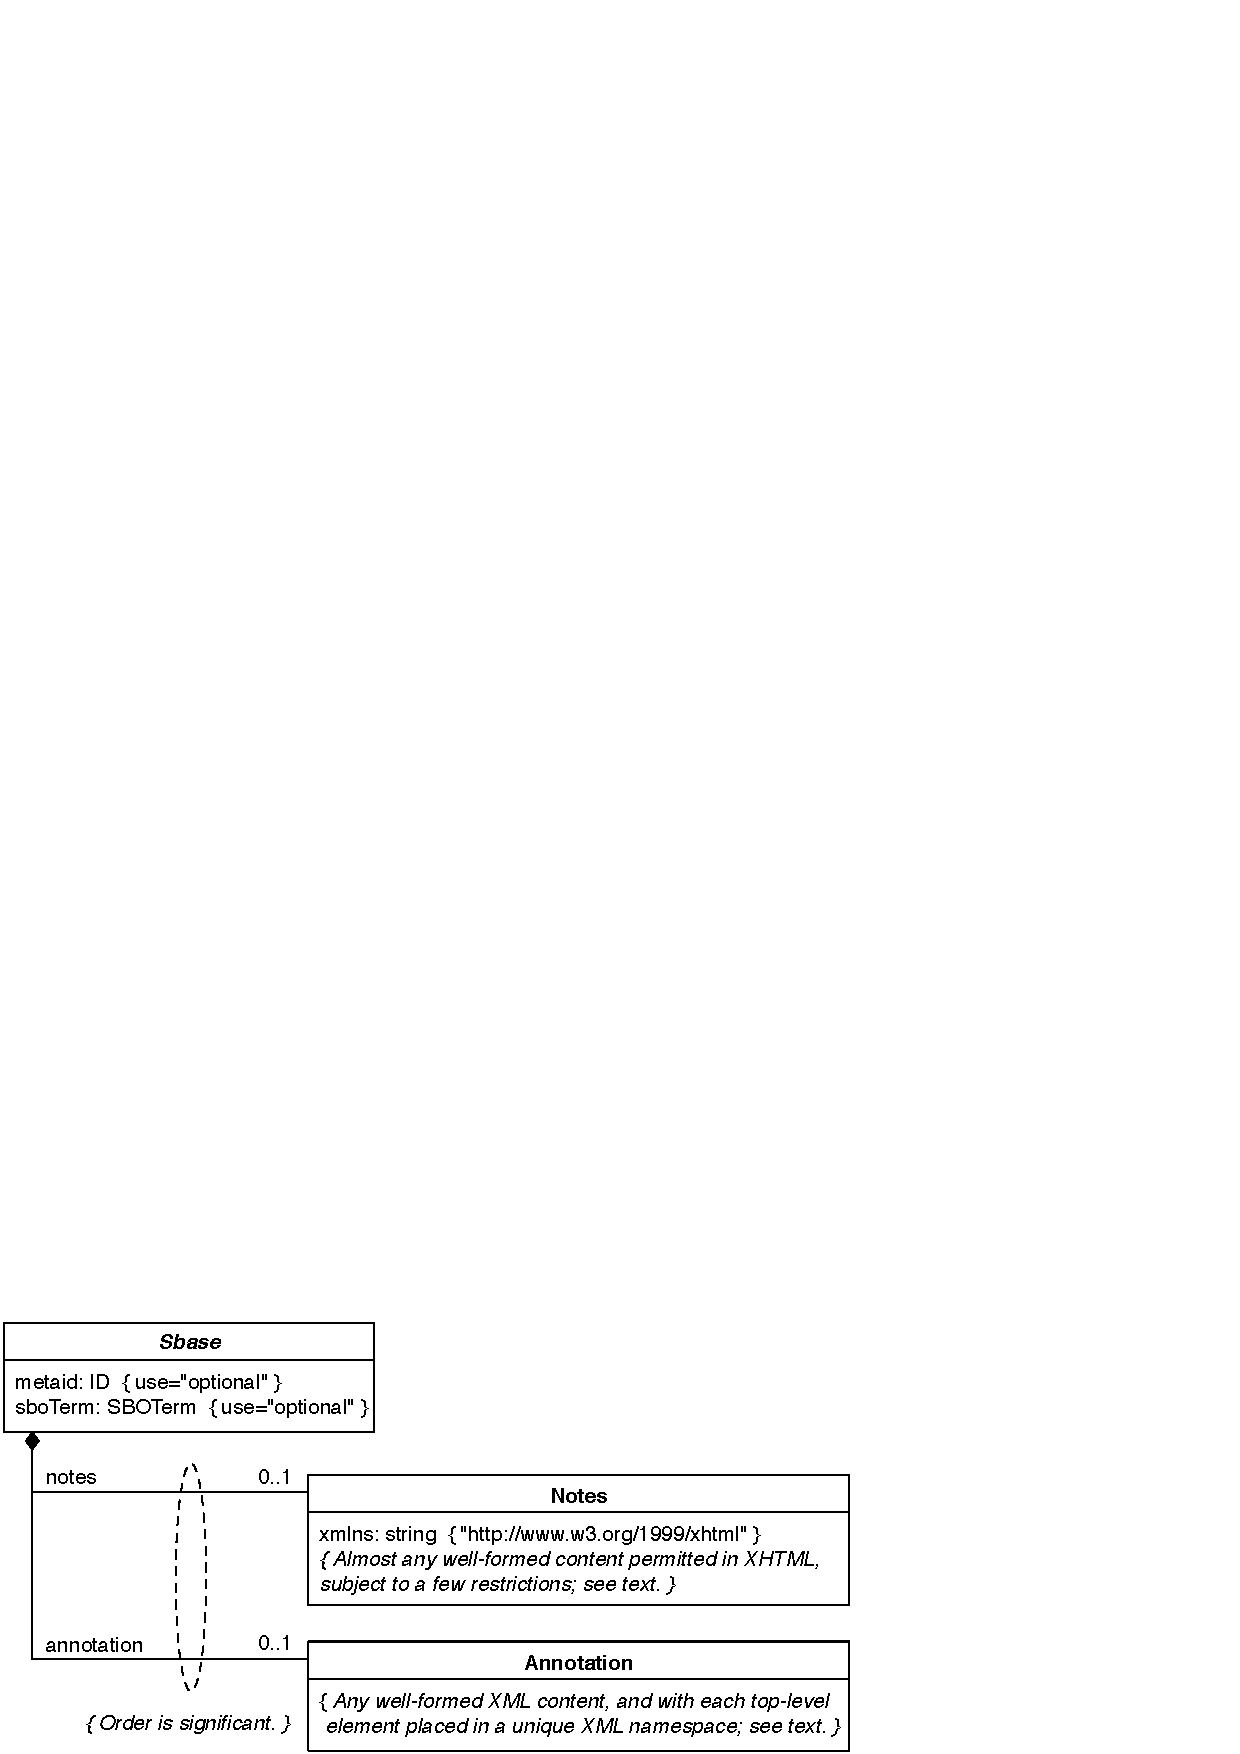
\includegraphics[scale=0.8]{figs/sbase-uml}
  \caption{The definition of \SBase.  Please refer to
    Section~\protect\ref{sec:notation} for a summary of the UML
    notation used here.  Note that the order of appearance of
    subelements \token{notes} and \token{annotation} is
    significant in instances of objects derived from
    \abstractclass{SBase}: \token{notes} must always come before
    \token{annotation}.}
  \label{fig:sbase}
\end{figure}

\SBase contains \changed{two attributes and two subelements}, all of which are optional:
\token{metaid}, \token{sboTerm}, \token{notes} and
\token{annotation}.  These are discussed separately in the
following subsections.


\subsubsection{The \token{metaid} \changed{attribute}}
\label{sec:metaid}

The \token{metaid} \changed{attribute} is present for supporting metadata
annotations using RDF~\citep[Resource Description
Format;][]{lassila:1999}.  It has a data type of XML \token{ID}
(the XML identifier type\changed{; see Section~\ref{sec:id}}), which means each \token{metaid} value
must be globally unique within an SBML file.  The \token{metaid}
value serves to identify a model component for purposes such as
referencing that component from metadata placed within
\token{annotation} \changed{elements} (see
Section~\ref{sec:annotation-use}).  Such metadata can use RDF
\token{description} elements, in which an RDF attribute called
\changed{\val{rdf:about} points to} the \token{metaid} identifier of an
object defined in the SBML model.  This topic is discussed in
greater detail in Section~\ref{sec:annotation-standard}.


\subsubsection{\changed{The \token{sboTerm} \changed{attribute}}}
\label{sec:sbase-sboterm}

The \changed{attribute} called \token{sboTerm} is provided on \SBase to support
the use of the Systems Biology Ontology (SBO; see
Section~\ref{sec:sbo}).  \changed{When a value is
given to this attribute, it} must conform to the data type
\primtype{SBOTerm} (Sections~\ref{sec:sboterm-type}).  SBO terms
are a type of optional annotation, and each different class of
SBML object derived from \SBase imposes its own requirements about
the values permitted for \token{sboTerm}.  Specific details on the
permitted values are provided with the definitions of SBML classes
throughout this specification document, and a broader discussion
is provided in Section~\ref{sec:sbo}.


\subsubsection{The \token{notes} \changed{element}}
\label{sec:notes}

The \changed{element} \token{notes} in \SBase is a container for
XHTML~1.0~\citep{pemberton:2002} content.  It is intended to serve
as a place for storing optional information intended to be seen by
humans.  An example use of the \token{notes} \changed{element} would be to
contain formatted user comments about the model \changed{element} in which
the \token{notes} \changed{element} is enclosed.  Every object derived
directly or indirectly from type \SBase can have a separate value
for \token{notes}, allowing users considerable freedom when adding
comments to their models.

XHTML~1.0 is simply a formulation of HTML~4 in XML~1.0.  This
means the full power of HTML formatting is available for use in
\token{notes} content.  The intention behind requiring XHTML
(rather than, for example, plain HTML or plain text) for
\token{notes} content is to balance several conflicting goals: (1)
choosing a format for notes that is compatible with the XML form of
SBML (plain HTML would not be); (2) supporting an international
formatting standard so that users have more control over the
appearance of notes and can predict to some degree how their notes
will be displayed in different tools and environments (which
argues against using plain-text notes); and (3) achieving these
goals using an approach that is hopefully easy enough for software
developers to support using off-the-shelf programming libraries.
It is worth noting in passing that the requirement for XHTML does
not \emph{prevent} users from entering plain-text content with
simple space/tab/newline formatting: it merely requires using the
standard \token{<pre>}...\token{</pre>} element of (X)HTML.

Modern libraries for displaying and editing (X)HTML content are
commonly available in contemporary software programming
environments, and software developers may wish to avail themselves
of these facilities rather than implementing their own XHTML
support systems.


\paragraph{XML Namespace requirements for \token{notes}}

The XML content of \token{notes} elements must declare the use of
the XHTML XML namespace.  This can be done in multiple ways.  One
way is to place a namespace declaration for the appropriate
namespace URI (which is \uri{http://www.w3.org/1999/xhtml}) on the
top-level \Sbml object (see Section~\ref{sec:sbml}) and then
reference the namespace in the \token{notes} content using a
prefix.  The following example illustrates this approach:

\begin{example}
<sbml xmlns="http://www.sbml.org/sbml/level2/version\changed{2}" level="2" version="\changed{2}"
      xmlns:xhtml="http://www.w3.org/1999/xhtml">
  ...
  <notes>
    <xhtml:body>
      <xhtml:center><xhtml:h2>A Simple Mitotic Oscillator</xhtml:h2></xhtml:center>
      <xhtml:p>A minimal cascade model for the mitotic oscillator
      involving cyclin and cdc2 kinase</xhtml:p>
    </xhtml:body>
  </notes>
  ...
\end{example}

Another approach is to declare the XHTML namespace within the
\token{notes} content itself, as in the following example:

\begin{example}
...
<notes>
  <body xmlns="http://www.w3.org/1999/xhtml">

    <center><h2>A Simple Mitotic Oscillator</h2></center>

    <p>A minimal cascade model for the mitotic oscillator
    involving cyclin and cdc2 kinase</p>

  </body>
</notes>
...
\end{example}

The \token{xmlns="http://www.w3.org/1999/xhtml"} declaration on
\token{body} as shown above changes the default XML namespace
within it, such that all of its content is by default in the XHTML
namespace.  This is a particularly convenient approach because it
obviates the need to prefix every element with a namespace prefix
(\eg \token{xhtml:center} as in the previous case).  Other
approaches are also possible.


\paragraph{The content of \token{notes}}

SBML does not require the content of \token{notes} to be any
particular XHTML element; the content can be almost any
well-formed XHTML content.  There are only two simple
restrictions.  The first restriction comes from the requirements
of XML: the \token{notes} element must not contain an XML
declaration nor a DOCTYPE declaration.  That is, \token{notes}
must \emph{not} contain

\begin{example}
<?xml version="1.0" encoding="UTF-8"?>  
\end{example}

nor (where the following is only one specific example of a
DOCTYPE declaration)

\begin{example}
<!DOCTYPE html PUBLIC "-//W3C//DTD XHTML 1.0 Strict//EN"
 "http://www.w3.org/TR/xhtml1/DTD/xhtml1-strict.dtd">
\end{example}

The second restriction is intended to balance freedom of content
with the complexity of implementing software that can interpret
the content.  The content of \token{notes} in SBML can consist
only of the following possibilities:
\begin{enumerate}
  
\item A complete XHTML document (minus the XML and DOCTYPE
  declarations, of course), that is, XHTML content beginning with
  the \token{html} tag.  The following is an example skeleton:
  \begin{example}
<notes>
    <html xmlns="http://www.w3.org/1999/xhtml">
      ...
    </html>
</notes>\end{example}

\item The \token{body} element from an XHTML document.  The
  following is an example skeleton:
  \begin{example}
<notes>
    <body xmlns="http://www.w3.org/1999/xhtml">
      ...
    </body>
</notes>\end{example}
  
\item Any XHTML content that would be permitted within a
  \token{body} element.  \changed{If} this consists of multiple
  elements, each one must declare the XML namespace separately.
  The following is an example \changed{fragment}:
  \begin{example}
<notes>
    <p xmlns="http://www.w3.org/1999/xhtml">
      ...
    </p>
    <p xmlns="http://www.w3.org/1999/xhtml">
      ...
    </p>
</notes>\end{example}

\end{enumerate}

Another way to summarize the restrictions above is simply to say
that the content of an SBML \token{notes} element can be only be a
complete \token{html} element, a \token{body} element, or whatever
is permitted inside a \token{body} element.  In practice, this
does not limit in any meaningful way what can be placed inside a
\token{notes} element; for example, if an application or modeler
wants to put a complete XHTML page, including a \token{head}
element, it can be done by putting in everything starting with the
\token{html} container.  However, the restrictions above do make
it somewhat simpler to write software that can read and write the
\token{notes} content.  Appendix~\ref{apdx:processing-notes}
describes one possible approach to doing just that.


\subsubsection{The \token{annotation} \changed{element}}
\label{sec:annotation-use}

Whereas the \token{notes} \changed{element} described above is a container for
content to be shown directly to humans, the \token{annotation}
\changed{element} is a container for optional software-generated content
\emph{not} meant to be shown to humans.  Every object derived
from \SBase can have its own value for \token{annotation}.  The
\changed{element's content} type is XML type \token{any}, allowing essentially
arbitrary data content.  SBML places only a few restrictions on
the organization of the content; these are intended to help
software tools read and write the data as well as help reduce
conflicts between annotations added by different tools.


\paragraph{The use of XML Namespaces in \token{annotation}}

% FIXME 2006-03-19:
% we should mention that RDF is an additional thing that can show
% up in annotations.  basically what's happening here is that we're
% saying any/all rdf content must be lumped together in one place

At the outset, software developers should keep in mind that
multiple software tools may attempt to read and write annotation
content.  To reduce the potential for collisions between
annotations written by different applications, \sbmltwothree
stipulates that tools must use XML namespaces~\citep{bray:1999} to
specify the intended vocabulary of every annotation.  The
application's developers must choose a URI (\emph{Universal
  Resource Identifier}; \citealt{harold:2001,w3c:2000}) reference
that uniquely identifies the vocabulary the application will use,
and a prefix string for the annotations.  Here is an example.
Suppose an application uses the URI \uri{http://www.mysim.org/ns}
and the prefix \token{mysim} when writing annotations related to
screen layout.  The content of an annotation might look like the
following:

\begin{example}
<annotation>
    <mysim:nodecolors xmlns:mysim="http://www.mysim.org/ns"
         mysim:bgcolor="green" mysim:fgcolor="white"/>
</annotation>
\end{example}

In this particularly simple case, the content consists of a single
XML element (\token{nodecolors}) with two attributes
(\token{bgcolor}, \token{fgcolor}), all of which are prefixed by
the string \token{mysim}.  (Presumably this particular content
would have meaning to the hypothetical application in question.)
The content in this particular example is small, but it should be
clear that there could easily have been an arbitrarily large
amount of data placed inside the \token{mysim:nodecolors} element.

The key point of the example above is that application-specific
annotation data is entirely contained inside a single
\emph{top-level element} within the SBML \token{annotation}
container.  SBML Level~2 Version~\changed{3} places the following
restrictions on annotations:
\begin{itemize}

\item Within a given SBML \token{annotation} element, there can
  only be one top-level element using a given namespace.  An
  annotation element can contain multiple top-level elements but
  each must be in a different namespace.

\item No top-level element in an \token{annotation} may use an
  SBML XML namespace, either explicitly by referencing one of the
  SBML XML namespace URIs or implicitly by failing to specify any
  namespace on the annotation.  \changed{As of \sbmltwothree, the
    defined SBML namespaces are the following URIs:}
  \begin{itemize}\setlength{\parskip}{-0.2ex}
  \item \uri{http://www.sbml.org/sbml/level1}
  \item \uri{http://www.sbml.org/sbml/level2}
  \item \uri{http://www.sbml.org/sbml/level2/version2}
  \item \changed{\uri{http://www.sbml.org/sbml/level2/version3}}
  \end{itemize}
  
\item The ordering of top-level elements within a given
  \token{annotation} element is \emph{not} significant.  An
  application should not expect that its annotation content
  appears first in the \token{annotation} element, nor in any
  other particular location.  \changed{Moreover, the ordering of
    top-level annotation elements may be changed by}
  \changed{different applications as they read and write the same
    SBML file.}

\end{itemize}

The use of XML namespaces in this manner is intended to improve
the ability of multiple applications to place annotations on SBML
model \changed{elements} with reduced risks of interference or name
collisions.  Annotations stored by different simulation packages
can therefore coexist in the same model definition.  The rules
governing the content of \token{annotation} elements are designed
to enable applications to easily add, change, and remove their
annotations from SBML elements while simultaneously preserving
annotations inserted by other applications when mapping SBML from
input to output.

\begin{blockChanged}

As a further simplification for developers of software and to
improve software interoperability, applications are only required
to preserve other annotations (i.e., annotations they do not
recognize) when those annotations are self-contained entirely
within \token{annotation}, complete with namespace declarations.
The following is an example:

\begin{example}
<annotation>
    <topLevelElement xmlns:"URI">
       \textrm{\emph{... content in the namespace identified by "URI"}...}
    </topLevelElement>
</annotation>
\end{example}

\end{blockChanged}

Some more examples hopefully will make \changed{these points} more clear.  The next
example is invalid because it contains a top-level element in the
SBML XML namespace---this happens because no namespace is declared
for the \token{<cytoplasm>} element, which means by default it
falls into the \changed{enclosing} SBML namespace:

\begin{example}
<annotation>
    <cytoplasm/>
</annotation>
\end{example}

The following example is \changed{also} invalid, \changed{this
  time} because it contains two top-level elements using the same
XML namespace.  Note that it does not matter that these are two
different top-level elements (\token{<nodecolors>} and
\token{<textcolors>}); what matters is that these separate
elements are both in the same namespace rather than having been
collected and placed inside one overall container element for that
namespace.

\begin{example}
<annotation>
    <mysim:nodecolors xmlns:mysim="http://www.mysim.org/ns"
        mysim:bgcolor="green" mysim:fgcolor="white"/>
    <mysim:textcolors xmlns:mysim="http://www.mysim.org/ns"
        mysim:bgcolor="green" mysim:fgcolor="white"/>
</annotation>
\end{example}

On the other hand, the following example is valid:

\begin{example}
<annotation>
    <mysim:geometry xmlns:mysim="http://www.mysim.org/ns"
             mysim:bgcolor="green" mysim:fgcolor="white">
        <graph:node xmlns:graph="http://www.graph.org/ns" 
             graph:x="4" graph:y="5" />
    </mysim:geometry>
    <othersim:icon xmlns:othersim="http://www.othersim.com/">
        WS2002
    </othersim:icon>
</annotation>
\end{example}

\begin{blockChanged}

For completeness, we note that annotations can legally be empty:

\begin{example}
<annotation />
\end{example}

\end{blockChanged}

It is worth keeping in mind that although XML namespace names must
be URIs, they are (like all XML namespace names) \emph{not
  required} to be directly usable in the sense of identifying an
actual, retrieval document or resource on the
Internet~\citep{bray:1999}.  URIs such as
\uri{http://www.mysim.org/} may appear as though they are (\eg)
Internet addresses, but there are not the same thing.  This style
of URI strings, using a domain name and other parts, is only a
simple and commonly-used way of creating a unique name string.

Finally, note that the namespaces being referred to here are XML
namespaces specifically in the context of the \token{annotation}
\changed{element} on \SBase.  The namespace issue here is unrelated to the
namespaces discussed in Section~\ref{sec:identifiers} in the
context of component identifiers in SBML.


\paragraph{Content of annotations and implications for software tools}

The \token{annotation} \changed{element} in the definition of \SBase exists in
order that software developers may attach optional
application-specific data to the \changed{elements} in an SBML model.
However, it is important that this facility not be misused.  In
particular, it is \emph{critical} that data essential to a model
definition or that can be encoded in existing SBML \changed{elements} is
\emph{not} stored in \token{annotation}. Parameter values,
functional dependencies between model \changed{elements}, etc., should not
be recorded as annotations.  It is crucial to keep in mind the
fact that data placed in annotations can be freely ignored by
software applications.  If such data affects the interpretation of
a model, then software interoperability is greatly impeded.

Here are examples of the kinds of data that may be appropriately
stored in \token{annotation}: (a) information about the graphical
layout of model components; (b) application-specific processing
instructions that do not change the essential meaning of a model;
(c) identification information for cross-referencing components in
a model with items in a data resource such as a database\changed{;
  and (d) information about the model that cannot} \changed{be
  readily encoded in existing SBML elements.}


\paragraph{Standardized format for certain classes of annotations}

\begin{blockChanged}

For case (c) above (i.e., cross-references between model
components and data resources, \sbmltwothree recommends a
standard format for use within \token{annotation}
\changed{elements}.  It should be used in preference to
proprietary syntaxes to maximize the likelihood that multiple
software tools will converge on the same syntax for this kind of
information.  The recommended scheme is described in
Section~\ref{sec:finney-novere}.

\end{blockChanged}


%-----------------------------------------------------------------------------
\subsection{The \token{id} and \token{name} \changed{attributes} on SBML components}
\label{sec:idnameattribs}
%-----------------------------------------------------------------------------

As will become apparent below, most \changed{objects} in SBML include two
common \changed{attributes}: \token{id} and \token{name}.  These \changed{attributes} are not
defined on \SBase (as explained in
Section~\ref{sec:why-not-on-sbase} below), but where they do
appear, the common rules of usage described below apply.


\subsubsection{The \token{id} \changed{attribute} and identifier scoping}
\label{sec:identifiers}

The \token{id} \changed{attribute is mandatory on most objects} in
SBML.  It is used to identify a component within the model
definition.  Other SBML \changed{objects} can refer to the component
using this identifier.  The data type of \token{id} is always
either \primtype{Sid} (Section~\ref{sec:sid}) or
\primtype{UnitSId} (Section~\ref{sec:unitsid}), depending on the
object in question.

A model can contain a large number of components representing
different parts.  This leads to a problem in deciding the scope of
an identifier: in what contexts does a given identifier \emph{X}
represent the same thing?  The approaches used in existing
simulation packages tend to fall into two categories which we may
call global and local.  The \emph{global} approach places all
identifiers into a single global space of identifiers, so that an
identifier \emph{X} represents the same thing wherever it appears
in a given model definition.  The \emph{local} approach places
symbols in separate identifier namespaces, depending on the
context, where the context may be, for example, individual
reaction rate expressions.  The latter approach means that a user
may use the same identifier \emph{X} in different rate expressions
and have each instance represent a different quantity.

The fact that different simulation programs may use different
rules for identifier resolution poses a problem for the exchange
of models between simulation tools.  Without careful
consideration, a model written out in SBML format by one program
may be misinterpreted by another program.  \sbmltwo must therefore
include a specific set of rules for treating identifiers and their
scopes.

The scoping rules in \sbmltwo are relatively
straightforward and are intended to avoid this problem with a
minimum of requirements on the implementation of software tools:
\begin{itemize}
  
\item The identifier (\ie the value of the \changed{attribute} \token{id}) of
  every \FunctionDefinition, \CompartmentType, \SpeciesType,
  \Compartment, \Species, \Parameter, \Reaction,
  \SpeciesReference, \ModifierSpeciesReference, \Event, and
  \Model, must be unique across the set of all such identifiers in
  the model.  This means, for example, that a reaction and a
  species definition cannot both have the same identifier.

\item The identifier of every \UnitDefinition must be unique
  across the set of all such identifiers in the model.  However,
  unit identifiers live in a separate space of identifiers from
  other identifiers in the model\changed{, by} \changed{virtue of
    the fact that the data type of unit identifiers is
    \primtype{UnitSId} (Section~\ref{sec:unitsid}) and not
    \primtype{SId}}.
  
\item Each \Reaction instance (see Section~\ref{sec:reactions})
  establishes a separate private local space for local \Parameter
  identifiers.  Within the definition of that reaction, local
  parameter identifiers override (shadow) identical identifiers
  outside of that reaction.  Of course, the corollary of this is
  that local parameters inside a \Reaction object instance are not
  visible to other objects outside of that reaction.

\end{itemize}
The set of rules above can enable software packages using either
local or global identifier spaces for parameters to exchange SBML
model definitions.  Software systems using local identifiers for
parameters internally should, in principle, be able to accept SBML
model definitions without needing to change component identifiers.
Environments using a common global space of identifiers for
parameters internally can perform manipulations of the identifiers
of local parameters within reaction definitions to avoid
identifier collisions.

The guidelines described here will hopefully provide a clean
transition path to future levels of SBML, when submodels are
introduced (Section~\ref{sec:level-3}).  Submodels will provide
the ability to compose one model from a collection of other
models.  This capability will have to be built on top of
\sbmltwo's namespace organization.  A straightforward approach to
handling namespaces is to make each submodel's space be private.
The rules governing identifier scoping within a submodel can
simply be the Level~2 namespace rule described here, with each
submodel having its own (to itself, global) namespace.


\subsubsection{The \token{name} \changed{attribute}}
\label{sec:name}

In contrast to the \token{id} \changed{attribute}, the \token{name} \changed{attribute} is
optional and is not intended to be used for cross-referencing
purposes within a model.  Its purpose instead is to provide a
human-readable label for the component.  The data type of 
\token{name} is the type \primtype{string} defined in XML
Schema~\citep{biron:2000,thompson:2000} and discussed further in
Section~\ref{sec:primitive-types}.  SBML imposes no restrictions
as to the content of \token{name} \changed{attributes} beyond those restrictions
defined by the \primtype{string} type in XML Schema.

The recommended practice for handling \token{name} is as follows.
If a software tool has the capability for displaying the content
of \token{name} \changed{attributes}, it should display this content to the user
as a component's label instead of the component's \token{id}.
If the user interface does not have this capability (e.g.,
because it cannot display or use special characters in symbol
names), or if the \token{name} \changed{attribute} is missing on a given
component, then the user interface should display the value of the
\token{id} \changed{attribute} instead.  (Script language interpreters are
especially likely to display \token{id} \changed{instead of}
\token{name}.)

As a consequence of the above, authors of systems that
automatically generate the values of \token{id} \changed{attributes} should be
aware some systems may display the \token{id}'s to the user.
Authors therefore may wish to take some care to have their
software create \token{id} values that are: (a) reasonably easy
for humans to type and read; and (b) likely to be meaningful, \eg
the \token{id} \changed{attribute} is an abbreviated form of the name \changed{attribute} value.

An additional point worth mentioning is although there are
restrictions on the uniqueness of \token{id} values (see
Section~\ref{sec:identifiers} above), there are no restrictions on
the uniqueness of \token{name} values in a model.  This allows
software packages leeway in assigning component identifiers.


\subsubsection{Why \token{id} and \token{name} are not defined on \class{SBase}}
\label{sec:why-not-on-sbase}

% [MH 2006-03-06] Most of the following issues could be addressed
% by having a separate "SBaseWithId" class.  I think only the first
% two reasons couldn't be addressed.  Thus, the original paragraph
% (which only talked about scoping) was almost in some sense the
% fundamental reason.  I added this other stuff to address some
% questions made in the past, but these other arguments are all
% trumped by saying ``just define an SBaseWithID''.  Therefore,
% it may be worth thinking about going back to the single reason.

Although many SBML components \changed{feature}
\token{id} and \token{name}, these \changed{attributes} are purposefully not defined on
\SBase.  There are several reasons for this.
\begin{itemize}
  
\item The presence of an SBML identifier \changed{attribute} (\token{id})
  necessarily requires specifying scoping rules for the
  corresponding identifiers.  However, the \SBase abstract type is
  used as the basis for defining components whose scoping rules
  are in some cases different from each other.  (See
  Section~\ref{sec:identifiers} for more details).  If \SBase were
  to have an \token{id} \changed{attribute}, then the specification of \SBase
  would need a default scoping rule and this would then have to be
  overloaded on derived classes that needed different scoping.
  This would make the SBML specification more complex.
  
\item Identifier are optional on some SBML components and required
  on most others.  If \token{id} were defined as optional on
  \SBase, most component classes would separately have to redefine
  \token{id} as being mandatory---hardly an improvement over the
  current arrangement.  Conversely, if \token{id} were defined as
  mandatory on \SBase, it would prevent it from being optional on
  components where it \emph{is} currently optional.
  
\item The \SBase abstract type is used as the base type for
  certain \changed{objects} such as \changed{\Sbml, \AssignmentRule},
  etc., which do not have identifiers because these components do
  not need to be referenced by other components.  If \SBase had a
  mandatory \token{id} \changed{attribute}, \emph{all} objects of
  these other types in a model would then need to be assigned
  unique identifiers.  Similarly, \changed{because \SBase is the
    base type of the \token{listOf\rule{0.5in}{0.5pt}} lists},
  putting \token{id} on \SBase would require all of these lists in
  a model to be given identifiers.  This would be a needless
  burden on software developers, tools, and SBML users, requiring
  them to generate and store additional identifiers for objects
  that never need them.
  
\item \SBase does not have a \token{name} simply because such an
  \changed{attribute} is always paired with an \token{id}.  Without
  \token{id} on \SBase, it does not make sense to have
  \token{name}.

\end{itemize}


%-----------------------------------------------------------------------------
\subsection{Mathematical formulas in SBML Level 2}
\label{sec:formulas}
%-----------------------------------------------------------------------------

Mathematical expressions in SBML Level~2 are represented using
\mathmltwo~\citep{w3c:2000b}.  MathML is an international standard
for encoding mathematical expressions using XML.  There are two
principal facets of MathML, one for encoding content (\ie the
semantic interpretation of a mathematical expression), and another
for encoding presentation or display characteristics.  SBML only
makes direct use of a subset of the content portion of MathML.  By
borrowing a separately-developed XML standard, we can avoid having
to define a specialized syntax for mathematical expressions in
SBML and simultaneously leverage existing intellectual and
technological work already done in the MathML community.  However,
it is not possible to produce a completely smooth and
conflict-free interface between MathML and other standards used by
SBML (in particular, \xmlschema).  Two specific issues and their
resolutions are discussed in Sections~\ref{sec:cn-token}.

The XML namespace URI for all MathML elements is
\uri{http://www.w3.org/1998/Math/MathML}.  Everywhere MathML
content is allowed in SBML, the MathML elements must be properly
placed within the \mathmltwo namespace.  In XML, this can be
accomplished in a number of ways, and the examples throughout this
specification illustrate the use of this namespace and MathML in
SBML.  Please refer to the W3C document by \citet{bray:1999} for
more technical information about using XML namespaces.


\subsubsection{Subset of MathML used in SBML Level 2}
\label{sec:mathmlsubset}

The subset of \mathmltwo elements used in SBML Level~2 is similar
to that used by CellML~\citep{hedley:2001b}, another model
definition language with similar goals as SBML.  The subset of
MathML elements used in SBML is listed below:
\begin{itemize}\setlength{\parskip}{-0.2ex}

\item \emph{token}: \token{cn}, \token{ci}, \token{csymbol},
  \token{sep}
  
\item \emph{general}: \token{apply}, \token{piecewise},
  \token{piece}, \token{otherwise}, \token{lambda} (the last is
  restricted to use in \FunctionDefinition)

\item \emph{relational operators}: \token{eq}, \token{neq},
  \token{gt}, \token{lt}, \token{geq}, \token{leq}

\item \emph{arithmetic operators}: \token{plus}, \token{minus},
  \token{times}, \token{divide}, \token{power}, \token{root},
  \token{abs}, \token{exp}, \token{ln}, \token{log},
  \token{floor}, \token{ceiling}, \token{factorial}

\item \emph{logical operators}: \token{and}, \token{or},
  \token{xor}, \token{not}

\item \emph{qualifiers}: \token{degree}, \token{bvar},
  \token{logbase}

\item \emph{trigonometric operators}: \token{sin}, \token{cos},
  \token{tan}, \token{sec}, \token{csc}, \token{cot},
  \token{sinh}, \token{cosh}, \token{tanh}, \token{sech},
  \token{csch}, \token{coth}, \token{arcsin}, \token{arccos},
  \token{arctan}, \token{arcsec}, \token{arccsc}, \token{arccot},
  \token{arcsinh}, \token{arccosh}, \token{arctanh},
  \token{arcsech}, \token{arccsch}, \token{arccoth}

\item \emph{constants}: \token{true}, \token{false},
  \token{notanumber}, \token{pi}, \token{infinity},
  \token{exponentiale}

\item \emph{annotation}: \token{semantics}, \token{annotation},
  \token{annotation-xml}

\end{itemize}
\vspace*{-0.75ex}
The inclusion of logical operators, relational operators,
\token{piecewise}, \token{piece}, and \token{otherwise} elements
facilitates the encoding of discontinuous expressions.  Note that
MathML elements for representing partial differential calculus are
not included.  We anticipate that the requirements for partial
differential calculus will be addressed in proposals for future
SBML geometry representations (see Section~\ref{sec:level-3}).

As defined by \mathmltwo, the semantic interpretation of the
mathematical functions listed above follows the definitions of the
functions laid out by \cite{abramowitz:1997} and
\cite{zwillinger:1988}.  Readers are directed to these sources and
the MathML specification for information about such things as
which principle values of the inverse trigonometric functions to
use.

Software authors should take particular note of the MathML
semantics of the N-ary operators \token{plus}, \token{times},
\token{and}, \token{or} and \token{xor}, when they are used with
different numbers of arguments.  The MathML
specification~\citep{w3c:2000b} appendix C.2.3 describes the
semantics for these operators with zero, one, and more arguments.

The following are the only attributes permitted on MathML elements
in SBML (in addition to the \token{xmlns} attribute on
\token{math} elements):
\begin{itemize}\setlength{\parskip}{-0.2ex}

\item \token{style}, \token{class} and \token{id} on any element;

\item \token{encoding} and \token{definitionURL} on
  \token{csymbol} elements; and

\item \token{type} on \token{cn} elements.

\end{itemize}\vspace*{-0.75ex}
Missing values for these attributes are to be treated in the same
way as defined by MathML.  These restrictions on attributes are
designed to confine the MathML elements to their default semantics
and to avoid conflicts in the interpretation of the type of token
elements.


\subsubsection{Numbers and \token{cn} elements}
\label{sec:cn-token}
\label{sec:mathml-value-space}

In MathML, literal numbers are written as the content portion of a
particular element called \token{cn}.  This element takes an
optional attribute, \token{type}, used to indicate the \emph{type}
of the number (such as whether it is meant to be an integer or a
floating-point quantity).  Here is an example of its use:
\begin{example}
<math xmlns="http://www.w3.org/1998/Math/MathML">
    <apply>
        <times/> <cn type="integer"> 42 </cn> <cn type="real"> 3.3 </cn>
    </apply>
</math>
\end{example}

The content of a \token{cn} element must be a number.  The number
can be preceded and succeeded by whitespace (see
Section~\ref{sec:mathml-whitespace}).  The following are the only
permissible values for the \token{type} attribute on MathML
\token{cn} elements: \val{e-notation}, \val{real}, \val{integer},
and \val{rational}.  The value of the \token{type} attribute
defaults to \val{real} if it is not specified on a given
\token{cn} element.


\paragraph{Value space restrictions on \token{cn} content}

SBML imposes certain restrictions on the value space of numbers
allowed in MathML expressions.  According to the \mathmltwo
specification, the values of the content of \token{cn} elements do
not necessarily have to conform to any specific floating point or
integer representations designed for CPU implementation.  For
example, in strict MathML, the value of a \token{cn} element could
exceed the maximum value that can be stored in a IEEE 64 bit
floating point number (IEEE 754).  This is different from the XML
Schema type \primtype{double} that is used in the definition of
floating point \changed{attributes} of \changed{objects} in SBML; the XML Schema
\primtype{double} \emph{is} restricted to IEEE double-precision
64-bit floating point type IEEE 754-1985.  To avoid an
inconsistency that would result between numbers elsewhere in SBML
and numbers in MathML expressions, \sbmltwothree imposes the
following restriction on MathML content appearing in SBML:
\begin{itemize}
  
\item Integer values (\ie the \changed{values} of \token{cn} elements
  having \token{type}=\val{integer} \changed{and both values in \token{cn} elements}
  \changed{having \token{type}=\val{rational}}) must conform to the
  \primtype{int} type used elsewhere in SBML
  (Section~\ref{sec:integer})
  
\item Floating-point values (\ie the content of \token{cn}
  elements having \token{type}=\val{real} or
  \token{type}=\val{e-notation}) must conform to the
  \primtype{double} type used elsewhere in SBML
  (Section~\ref{sec:double})
\end{itemize}


\paragraph{Syntactic differences in the representation of numbers
  in scientific notation}

It is important to note that MathML uses a style of scientific
notation that differs from what is defined in XML Schema, and
consequently what is used in SBML attribute values.  The
\mathmltwo type \val{e-notation}
\changed{(as} \changed{well as the type \val{rational})}
requires the mantissa and
exponent to be separated by one \texttt{<sep/>} element.  The
mantissa must be a real number and the exponent part must be a
signed integer.  This leads to expressions such as

\begin{example}
<cn type="e-notation"> 2 <sep/> -5 </cn>
\end{example}

for the number $2 \times 10^{-5}$.  It is especially
important to note that the expression

\begin{example}
<cn type="e-notation"> 2e-5 </cn>
\end{example}

is \emph{not valid} in \mathmltwo and therefore cannot be used in
MathML content in SBML.  However, elsewhere in SBML, when an
attribute value is declared to have the data type
\primtype{double} (a type taken from XML Schema), the compact
notation \val{2e-5} is in fact allowed.  In other words, within
MathML expressions contained in SBML (and \emph{only} within such
MathML expressions), numbers in scientific notation must take the
form \token{<cn type="e-notation"> 2 <sep/> -5 </cn>}, and
everywhere else they must take the form \val{2e-5}.

This is a regrettable difference between two standards that SBML
replies upon, but it is not feasible to redefine these types
within SBML because the result would be incompatible with parser
libraries written to conform with the MathML and XML Schema
standards.  It is also not possible to use XML Schema to define a
data type for SBML attribute values permitting the use of the
\token{<sep/>} notation, because XML attribute values cannot
contain XML elements---that is, \token{<sep/>} cannot appear in an
XML attribute value.


\begin{blockChanged}

\paragraph{Units of numbers in MathML \token{cn} expressions}
\label{sec:units-of-mathml}

What units should be attributed to values appearing inside MathML
\token{cn} elements?  One answer is to assume that the units
should be ``whatever units appropriate in the context where the
number appears''.  This implies that units can always be assigned
unambiguously to any number appearing in any expression, and this
turns out to be false.  Another answer is that numbers should be
considered ``dimensionless''.  This may be correct in pure
mathematics and other contexts, but it turns out that when numbers
appear in expressions in SBML's domain of application, they are
rarely \emph{intended} to have the units \val{dimensionless} even
if the units are not declared: they are \emph{supposed} to have
specific units, but the units are usually undeclared.  (Being
\changed{``dimensionless'' is} not the same as having
\emph{undeclared} units!)  More importantly, for SBML to define
numbers as being \emph{by default} dimensionless would likely
result in many models being technically incorrect without the
modeler being aware of it unless their software tools performed
dimensional analysis.  Most software tools today still do not, and
so the discovery of incorrect units would not occur until other
researchers and database curators attempted to use the model in
software packages that did check units.

The current approach in SBML is to leave the default units of
numbers undefined.  Software packages and modelers are encouraged
to explicitly add unit declarations to numbers; such declarations
can permit software tools to perform dimensional analysis and
potentially report model errors.  There are (at least) two simple
methods for associating units with numerical quantities in SBML:

\begin{itemize}

\item Do not use literal numbers at all; instead, define
  \Parameter objects (Section~\ref{sec:parameters}) for every
  quantity, and declare units for each such parameter in its
  definitions.  (This is the best modeling practice anyway.)

\item Define separate parameters for the needed units, such that
  the parameters have numerical values of \val{1} and the
  appropriate units assigned via their \token{units} attribute.
  Parameters are described in detail in
  Section~\ref{sec:parameters}, but to foreshadow them, here is an
  example:
  \begin{example}
    <listOfParameters>
        <parameter id="SubstanceUnits" value="1" units="substance"/>
    </listOfParameters>\end{example}

  Numbers that need to be in the model's substance units can then
  be assigned those units by multiplying the number with the
  parameter defined above using standard MathML.  The numerical
  value will be left unchanged because the value of the parameter
  is the multiplicative identity \val{1}.  For example:
  \begin{example}
    <apply>
        <times/>
        <cn> 2 </cn>
        <ci> SubstanceUnits </ci>
    </apply>\end{example}\vspace*{-1ex}

\end{itemize}

\end{blockChanged}


\subsubsection{Use of \token{ci} elements in MathML expressions in SBML}
\label{sec:ci-token}

The content of a \token{ci} element must be an SBML identifier
that is declared elsewhere in the model.  The identifier can be
preceded and succeeded by whitespace. The set of possible
identifiers that can appear in a \token{ci} element depends on the
containing \changed{element} in which the \token{ci} is used:
\begin{itemize}
  
\item If a \token{ci} element appears in the body of a
  \FunctionDefinition object
  (Section~\ref{sec:functiondefinition}), the referenced
  identifier must be either (i) one of the declared arguments to
  that function, or (ii) the identifier of a previously defined
  \changed{\FunctionDefinition object} in the model.
  
\item Otherwise, the referenced identifier must be that of a
  \Species, \Compartment, \Parameter, \FunctionDefinition, or
  \Reaction object defined in the model.  The following are the
  only possible interpretations of using such an identifier in
  SBML:
  \begin{itemize}
    
  \item \emph{Species identifier}: When a \Species identifier
    occurs in a \token{ci} element, it represents the quantity of
    that species in terms of either \quantity{amount of substance}
    units or in terms of \quantity{concentration} units, depending
    on the definition of that species; see
    Section~\ref{sec:species-units}.
    
  \item \emph{Compartment identifier}: When a \Compartment
    identifier occurs in a \token{ci} element, it represents the
    size of the compartment.  The units associated with the size
    of the compartment are those given on the \Compartment
    \changed{element} that declares the identifier; see
    Section~\ref{sec:compartment-units}.
    
  \item \emph{Parameter identifier}: When a \Parameter identifier
    occurs in a \token{ci} element, it represents the numerical
    value assigned to that parameter.  The units associated with
    the parameter's value are the units assigned in the instance
    of the \Parameter \changed{element}; see
    Section~\ref{sec:parameter-units}.
    
  \item \emph{Function identifier}: When a \FunctionDefinition
    identifier occurs in a \token{ci} element, it represents a
    call to that function.  Function references in MathML occur in
    the context of using MathML's \token{apply} and often involve
    supplying arguments to the function; see
    Section~\ref{sec:functiondefinition}.  \changed{The units
      associated} \changed{with the value returned by the function
      call are the overall units of the mathematical expression}
      \changed{contained in the function definition.}
    
  \item \emph{Reaction identifier}: When a \Reaction identifier
    occurs in a \token{ci} element, it represents the rate of that
    reaction as determined by the mathematical formula in the
    \KineticLaw object within the \Reaction.  The units associated
    with the reaction are \quantity{substance}/\quantity{time},
    with the \quantity{substance} and \quantity{time} units
    established by the values of the SBML built-in units
    \val{substance} and \val{time}, respectively.  These units may
    be redefined in model; see Section~\ref{sec:built-in-units}.
    If the reaction definition has no \KineticLaw, the use of the
    reaction identifier is an error (perhaps indicating that the
    model is incomplete).

  \end{itemize}

\end{itemize}

The content of \token{ci} elements in MathML formulas outside of a
\KineticLaw or \FunctionDefinition must always refer to objects
declared in the top level global namespace; \ie SBML uses ``early
binding'' semantics.  Inside of \KineticLaw, a \token{ci} element
can additionally refer to local parameters defined within that
\KineticLaw instance; see Section~\ref{subsec:kinetic-law} for
more information.


\begin{blockChanged}

\subsubsection{Interpretation of boolean values}
\label{sec:handling-booleans}

As noted already in Section~\ref{sec:boolean}, there is another
unfortunate difference between the \xmlschemaone and \mathmltwo
standards that impacts mathematical expressions in SBML: in
\xmlschema, the value space of type \primtype{boolean} includes
\val{true}, \val{false}, \val{1}, and \val{0}, whereas in
\mathml, only \val{true} and \val{false} count as boolean
values.

The impact of this difference thankfully is minimal because the
\xmlschema definition is only used for attribute values on SBML
objects, and those values turn out never to be accessible from
\mathml content in SBML---values of boolean \changed{attributes} on SBML objects
can never enter into \mathml expressions.  Nevertheless, software
authors and users should be aware of the difference and in
particular that \val{0} and \val{1} are interpreted as numerical
quantities in mathematical expressions.  There is no automatic
conversion of \val{0} or \val{1} to boolean values in contexts
where booleans are expected.  This allows stricter type checking
and unit verification during validation of models.

\end{blockChanged}


\subsubsection{Handling of whitespace}
\label{sec:mathml-whitespace}

\mathmltwo defines ``whitespace'' in the same way as XML does, \ie
the space character (Unicode hexadecimal code 0020), horizontal
tab (code 0009), newline or line feed (code 000A), and carriage
return (code 000D).  In MathML, the content of elements such as
\token{cn} and \token{ci} can be surrounded by whitespace
characters.  Prior to using the content, this whitespace is
``trimmed'' from both ends: all whitespace at the beginning and
end of the content is removed~\citep{ausbrooks:2003}.  For
example, in \texttt{<cn> 42 </cn>}, the amount of white space on
either side of the ``\texttt{42}'' inside the \texttt{<cn>}
\ldots\ \texttt{</cn>} container does not matter.  Prior to
interpreting the content, the whitespace is removed altogether.


\subsubsection{Use of \token{csymbol} elements in MathML expressions in SBML}
\label{sec:csymbol-token}

SBML Level 2 uses the MathML \token{csymbol} element to denote
certain built-in mathematical entities without introducing
reserved names into the component identifier namespace.  The
\token{encoding} \changed{attribute} of \token{csymbol} \changed{must} be set to
\val{text}.  The \token{definitionURL} should be set to one of the
following predefined SBML symbol URIs:
\begin{itemize}

\item \uri{http://www.sbml.org/sbml/symbols/time}.  This
  represents the current simulation time.  See
  Section~\ref{sec:meaning-of-time} for more information.  The
  units of the current time entity are determined from the
  built-in \token{time} of Table~\vref{tab:builtin}.

\item \uri{http://www.sbml.org/sbml/symbols/delay}.  This
  represents a delay function.  The delay function has the form
  $delay(x, d)$, taking two MathML expressions as arguments.  Its
  value is the value of argument $x$ at $d$ time units before the
  current time.  There are no restrictions on the form of $x$.
  The units of the $d$ parameter are determined from the built-in
  \token{time}.  The value of the $d$ parameter, when evaluated,
  must be numerical (\ie a number in MathML real, integer, or
  ``e-notation'' format) and be greater than or equal to 0.  The
  \emph{delay} function is useful for representing biological
  processes having a delayed response, but where the detail of the
  processes and delay mechanism is not relevant to the operation
  of a given model.  See Section~\ref{sec:meaning-of-time} below
  for additional considerations surrounding the use of this
  \token{csymbol}.

\end{itemize}

The following examples demonstrate these concepts.  The XML fragment below
encodes the formula $x + t$, where $t$ stands for time.

\begin{example}
<math xmlns="http://www.w3.org/1998/Math/MathML">
    <apply>
        <plus/>
        <ci> x </ci>
        <csymbol encoding="text" definitionURL="http://www.sbml.org/sbml/symbols/time">
            t
        </csymbol>
    </apply>
</math>
\end{example}

In the fragment above, the use of the token \token{t} is mostly a
convenience for human readers---the string inside the
\token{csymbol} could have been almost anything, because it is
essentially ignored by MathML parsers and SBML.  Some MathML and
SBML processors will take note of the token and use it when
presenting the mathematical formula to users, but the token used
has no impact on the interpretation of the model and it does
\emph{not} enter into the SBML component identifier namespace.  In
other words, the SBML model cannot refer to \token{t} in the
example above.  The content of the \token{csymbol} element is for
rendering purposes only and can be ignored by the parser.

As a further example, the following XML fragment encodes the equation
$k + delay(x, 0.1)$ or alternatively $k_t + x_{t - 0.1}$:

\begin{example}
<math xmlns="http://www.w3.org/1998/Math/MathML">
    <apply>
        <plus/>
        <ci> k </ci>
        <apply>
            <csymbol encoding="text" definitionURL="http://www.sbml.org/sbml/symbols/delay">
                delay
            </csymbol>
            <ci> x </ci>
            <cn> 0.1 </cn>
        </apply>
    </apply>
</math>
\end{example}

Note that the URI in the value of \token{definitionURL}, as all
URIs, is intended to serve as a unique identifier and is not
intended to be dereferenced as an Internet address.  There is
nothing actually located at the address
\uri{http://www.sbml.org/sbml/symbols/delay}.


\subsubsection{Simulation time}
\label{sec:meaning-of-time}

The principal use of SBML is to represent quantitative dynamical
models whose behaviors manifest themselves over time.  In defining
an SBML model using constructs such as reactions, time is most
often implicit and does not need to be referred to in the
mathematical expressions themselves.  However, sometimes an
explicit time dependency needs to be stated, and for this purpose,
the \emph{time} \token{csymbol} (described above in
Section~\ref{sec:csymbol-token}) may be used.  This \emph{time}
symbol refers to ``instantaneous current time'' in a simulation,
frequently given the literal name $t$ in one's equations.

An assumption in SBML is that ``start time'' or ``initial time''
in a simulation is zero, that is, if $t_0$ is the initial time in
the system, $t_0 = 0$.  This corresponds to the most common
scenario.  Initial conditions in SBML take effect at time $t = 0$.
There is no mechanism in SBML for setting the initial time to a
value other than 0.  To refer to a different time in a model, one
approach is to define a \Parameter for a new time variable and use
an \AssignmentRule in which the assignment expression subtracts a
value from the \token{csymbol} \emph{time}.  For example, if the
desired offset is 2 time units, the MathML expression would be

\begin{example}
<math xmlns="http://www.w3.org/1998/Math/MathML">
    <apply>
        <minus/>
        <csymbol encoding="text" definitionURL="http://www.sbml.org/sbml/symbols/time"> t
        </csymbol>
        <cn> 2 </cn>
    </apply>
</math>
\end{example}

SBML's assignment rules (Section~\ref{sec:assignmentrule}) can be
used to express mathematical statements that hold true at all
moments, so using an assignment rule with the expression above
will result in the value being equal to $t - 2$ at every point in
time.  A parameter assigned this value could then be used
elsewhere in the model, its value could be plotted by a simulator,
etc.


\subsubsection{Initial conditions and special considerations}
\label{sec:before-t0}

The identifiers of \Species, \Compartment, \Parameter, and
\Reaction object instances in a given SBML model refer to the main
variables in a model.  Depending on certain attributes of these
objects (\eg the \changed{attribute} \token{constant} on species, compartments
and parameters---this and other conditions are explained in the
relevant sections elsewhere in this document), some of the
variables may have constant values throughout a simulation, and
others' values may change.  These changes in values over time are
determined by the system of equations constructed from the model's
reactions, initial assignments, rules, and events.

As described in Section~\ref{sec:meaning-of-time}, an SBML model's
simulation is assumed to begin at $t = 0$.  The availability of
the \emph{delay} \token{csymbol} (Section~\ref{sec:csymbol-token})
introduces the possibility that at $t \geq 0$, mathematical
expressions in a model may draw on values of model components from
time \emph{prior} to $t = 0$.  A simulator may therefore need to
compute the values of variables at time points $t_i \leq 0$ to
allow the calculation of values required for the evaluation of
delay expressions in the model for $t \geq 0$.  If there are no
delays in the model, then $t_i = 0$.

The following is how the definitions of the model should be
applied:
\begin{enumerate}

\item At time $t_i$:
  \begin{itemize}
    
  \item Every \Species, \Compartment, and \Parameter whose
    definition includes an initial value is assigned that value.
    If an \changed{element has} \token{constant}=\val{false}, its
    value may be changed by other constructs or reactions in a
    model according to the steps below; if
    \token{constant}=\val{true}, only an \InitialAssignment can
    override the value.
    
  \item All \InitialAssignment definitions take effect at $t_i$
    and continue to have effect up to and including $t = 0$,
    overriding any initial values on \Species, \Compartment and
    \Parameter.  Since \InitialAssignment{}s contain mathematical
    formulas, different values may be computed at each time step
    $t$ in $t_i \leq t \leq 0$.

%    The value of every \Species, \Compartment, and \Parameter    
%    object whose identifier is \emph{not} the subject of an
%    \InitialAssignment is assigned by the definition of that
%    object in the model; conversely, the value of every \Species,
%    \Compartment, and \Parameter object whose identifier \emph{is}
%    the subject of an \InitialAssignment is computed and assigned
%    by that \InitialAssignment.  
%    All assignments of both kinds are
%    performed once and thereafter are in effect for $t \geq t_i$.

  \end{itemize}
  
\item For time $t \geq t_i$:
  \begin{itemize}
    
  \item \AssignmentRule and \AlgebraicRule definitions are in
    effect from this point in time forward and may influence the
    values of \Species quantity, \Compartment size, and \Parameter
    values.  (Note there cannot be both an \AssignmentRule and an
    \InitialAssignment for the same identifier; see
    Section~\ref{sec:rules}.)

  \end{itemize}
  
\item At time $t = 0$:
  \begin{itemize}  
    
  \item The system of equations constructed by combining
    \AssignmentRule equations, \AlgebraicRule equations, \RateRule
    equations, and the equations constructed from the \Reaction
    definitions in the model, are used to obtain consistent
    initial conditions for numerical solver algorithms.  (Note
    that there cannot be both an \AssignmentRule and a \RateRule
    for the same identifier, or both an \AssignmentRule and an
    \InitialAssignment for the same identifier; see
    Section~\ref{sec:assignmentrule}.)
    
  \item \Constraint definitions begin to take effect (and a
    constraint violation may result; see
    Section~\ref{sec:constraints}).

  \end{itemize}
  
\item For time $t > 0$:
  \begin{itemize}
    
  \item \RateRule definitions can begin to take effect.
    
  \item \Event definitions can begin to take effect.  (Note that
    an \Event cannot be defined to change the value of a variable
    that is also the subject of an \AssignmentRule; see
    Section~\ref{sec:events}.)

  \item System simulation proceeds.

  \end{itemize}

\end{enumerate}  

To reiterate: in modeling situations that do not involve the use
of the \emph{delay} \token{csymbol}, $t_i = 0$, but this does not
alter the steps above.


\subsubsection{\changed{MathML} expression \changed{data} types}
\label{sec:mathmltype}

MathML operators in SBML each return results in one of two
possible types: boolean and numerical.  \changed{By}
\changed{\emph{numerical} type, we mean either (1) a number in
  MathML real, integer, rational, or ``e-notation'' format;}
\changed{or (2) the \token{csymbol} for delay or the
  \token{csymbol} for time described in
  Section~\ref{sec:csymbol-token}.}  The following guidelines
summarize the different possible cases.

The relational operators (\token{eq}, \token{neq}, \token{gt},
\token{lt}, \token{geq}, \token{leq}), the logical operators
(\token{and}, \token{or}, \token{xor}, \token{not}), and the
boolean constants (\token{false}, \token{true}) always return
boolean values.  \changed{As noted in
  Section~\ref{sec:handling-booleans}, the numbers \token{0} and
  \token{1} do} \changed{not count as boolean values in \mathml
  contexts in SBML.}

The type of an operator referring to a \FunctionDefinition is
determined by the type of the top-level operator of the expression
in the \token{math} \changed{element} of the \FunctionDefinition
instance, and can be boolean or numerical.

All other operators, values and symbols return numerical
results.

The roots of the expression trees used in the following contexts
must yield boolean values:

\begin{itemize}\setlength{\parskip}{-0.2ex}

\item the arguments of the MathML logical operators (\token{and},
\token{or}, \token{xor}, \token{not});

\item the second argument of a MathML \token{piece} operator;

\item the \token{trigger} \changed{element} of an SBML \Event; and

\item the \token{math} \changed{element} of an SBML \Constraint.

\end{itemize}

The roots of the expression trees used in the following contexts can
optionally yield boolean values:

\begin{itemize}\setlength{\parskip}{-0.2ex}

\item the arguments to the \token{eq} and \token{neq} operators;

\item the first arguments of MathML \token{piece} and \token{otherwise}
operators; and

\item the top level expression of a function definition.

\end{itemize}

The roots of expression trees in other contexts must yield
numerical values.

The type of expressions should be used consistently.  The set of
expressions that make up the first arguments of the \token{piece}
and \token{otherwise} operators within the same \token{piecewise}
operator should all return values of the same type. The arguments
of the \token{eq} and \token{neq} operators should return the same
type.

\begin{blockChanged}

\subsubsection{Units of arguments to mathematical operators}
\label{sec:operator-arg-types}

The units associated with the arguments to operators such as
\token{plus} and \token{power} should be made mathematically and
physically sensible.  Many mathematical operators cannot be
applied to arguments that have units of physical dimensions---the
operators are technically defined in terms of dimensionless
quantities.  (For example, it is not clear what would be the
interpretation of taking the natural logarithm of a quantity
having units of length.)  Thus, the following rules should be
followed for the units of arguments to MathML operators in SBML:
\begin{itemize}

\item All arguments to the following operators should have the
  same units (regardless of what those units happen to be):
  \token{plus}, \token{minus}, \token{eq}, \token{neq} \token{gt},
  \token{lt}, \token{geq}, \token{leq}.

\item The units of each argument to the following operators should
  be \val{dimensionless}: \token{exp}, \token{ln}, \token{log},
  \token{factorial}, \token{sin}, \token{cos}, \token{tan},
  \token{sec}, \token{csc}, \token{cot}, \token{sinh},
  \token{cosh}, \token{tanh}, \token{sech}, \token{csch},
  \token{coth}, \token{arcsin}, \token{arccos}, \token{arctan},
  \token{arcsec}, \token{arccsc}, \token{arccot}, \token{arcsinh},
  \token{arccosh}, \token{arctanh}, \token{arcsech},
  \token{arccsch}, \token{arccoth}.

\item The units of the argument to the operators \token{abs},
  \token{floor} and \token{ceiling} can be anything.

\item The units of each argument in a call to a
  \FunctionDefinition should match the units expected by the
  \token{lambda} expression within the \token{math} expression of
  that \FunctionDefinition instance.

\item The two arguments to \token{power}, which are of the form
  $\textit{power}(a,b)$ with the meaning $a^b$, should be as
  follows: (1) if the second argument is an integer, then the
  first argument can have any units; (2) if the second argument
  $b$ is a rational number $n/m$, it must be possible to derive
  the $m$-th root of $(a \{\text{unit}\})^n$, where
  $\{\text{unit}\}$ signifies the units associated with $a$;
  otherwise, (3) the units of the first argument must be
  \val{dimensionless}.  The second argument ($b$) should always
  have units of \val{dimensionless}.

\item The two arguments to \token{root}, which are of the form
  $\textit{root}(n,a)$ with the meaning $\sqrt[n]{a}$ and where
  the degree $n$ is optional (defaulting to \val{2}), should be as
  follows: (1) if the optional degree qualifier $n$ is an integer,
  then it must be possible to derive the $n$-th root of $a$; (2)
  if the optional degree qualifier $n$ is a rational $n/m$ then it
  must be possible to derive the $n$-th root of $(a
  \{\text{unit}\})^m$, where $\{\text{unit}\}$ signifies the units
  associated with $a$; otherwise, (3) the units of $a$ must be
  \val{dimensionless}.

\item All of the possible return values from \token{piece} and
  \token{otherwise} subelements of a \token{piecewise} expression
  should have the same units, regardless of what those units are.
  (Otherwise, the \token{piecewise} expression would return values
  having different units depending on which case evaluated to
  true.)

\item For the \emph{delay} \token{csymbol}
  (Section~\ref{sec:csymbol-token}) function, which has the form
  $delay(x, d)$, the second argument $d$ should have units of time.

\end{itemize}

We advise declaring the units of all quantities in a model,
insofar as this is possible, using the various mechanisms provided
for this in SBML.  Fully declared units can allow software tools
to perform dimensional analysis on the units of mathematical
expressions, and such analysis can be valuable in helping modelers
produce correct models.  The lack of declared units on quantities
in a model does not render it invalid SBML, but it reduces the
types of consistency checks that software packages can perform.


% fixme: add smth about this:
%
% I know that people use the above and it is perfectly fine as long as [A]
% has units dimensionless. If the unit is not dimensionless the above is
% nonsense. I think we decided to allow nonsense but mark the model as
% yellow when we are able to detect it. I know that it sounds strange to
% have valid, invalid and suspicious models but I think that is the way we
% need to go at least at the moment. In addition, the above can be easily
% corrected. 
%   k' * ([A]/(substance_unit/volume_unit))^pi.


\end{blockChanged}


% Restore normal printing of section headings (without coloring).
% See earlier in this file where these commands were redefined to
% print section headings in red for this part of the document.

\makeatletter
\renewcommand{\thesection}      {\@arabic\c@section}
\renewcommand{\thesubsection}   {\thesection.\@arabic\c@subsection}
\renewcommand{\thesubsubsection}{\thesubsection .\@arabic\c@subsubsection}
\renewcommand{\theparagraph}    {\thesubsubsection.\@arabic\c@paragraph}
\makeatother

% -*- TeX-master: "sbml-level-3-version-2-core"; fill-column: 66 -*-
% ----------------------------------------------------------------

\section{SBML components}
\label{sec:elements}

In this section, we define each of the major components of SBML.
We use the UML notation described in
Section~\ref{sec:notation-uml} for defining classes of objects.
We also illustrate the use of SBML components by giving partial
model definitions in XML.  Section~\ref{sec:xml-rep} provides many
complete example models encoded in SBML.


%-----------------------------------------------------------------------------
\subsection{The SBML container}
\label{sec:sbml}
%-----------------------------------------------------------------------------

All well-formed SBML documents must begin with an \emph{XML
  declaration}, which specifies both the version of XML assumed
and the document character encoding.  The declaration begins with
the characters \token{<?xml} followed by the XML \token{version}
and \token{encoding} attributes.  SBML \thisL uses XML version 1.0
and requires a document encoding of UTF-8.  Following this
declaration, the outermost portion of a model expressed in \thisL
consists of an object of class \SBML, defined in
Figure~\ref{fig:sbml}.  This class contains three required
attributes (\token{level}, \token{version} and \token{xmlns}), and
a required \token{model} element.

\begin{figure}[htb]
  \centering
  \small
  \begin{tikzpicture}[level distance=0.5in]
  \node { \emptyClassbox{\textsl{SBase}} }
    [open triangle 60-,edge from parent fork down,sibling distance=3.25in]
    child {node[below=-10pt] (a) {
        \begin{classbox}{SBML}
          xmlns: string \{ use=\texttt{"}required\texttt{"} fixed=\texttt{"}http://www.sbml.org/sbml/level3/\verdiff{version1}{version2}/core\texttt{"} \} \\
          level: positiveInteger \{ use=\texttt{"}required\texttt{"} fixed=\texttt{"}3\texttt{"} \}   \\
          version: positiveInteger \{ use=\texttt{"}required\texttt{"} fixed=\texttt{"}\verdiff{1}{2}\texttt{"} \} \\
          \{ \emph{Additional attributes permitted.} \} \\
        \end{classbox}
      }}
    child {node[below=13pt] (b) {
        \emptyClassbox{Model}
      }}
   ;
   \draw[diamond-, above=0pt] (a) -- (b) 
     node[above=6pt,left=0.6in] {\textsf{model}}
     node[above=6pt,left=0.25in] {\verdiff{}{\textsf{0..1}}};
\end{tikzpicture}\vspace*{-1em}
%
  \vspace{1.5ex}
  \caption{The definition of class \SBML for SBML \thisLV.  The
    class \Model is defined in Section~\ref{sec:model}.  Note that
    \SBML and \Model are subclasses of \SBaseUpright, and therefore
    inherit the attributes of that abstract class.}
  \label{fig:sbml}
\end{figure}

The \SBML class defines the structure and content of the
\token{sbml} outermost element in an SBML file.  The following is
an abbreviated example of an \SBML class object translated into
XML form for an SBML Level~3 Version~1 Core document (and here,
ellipses are used to indicate content elided from this example):

\begin{example}
<?xml version="1.0" encoding="UTF-8"?>
<sbml xmlns="http://www.sbml.org/sbml/level3/version1/core" level="3" version="1">
  ...
  <model ...>
     ...
  </model>
</sbml>
\end{example}

The attribute \token{xmlns} declares the XML namespace used within
the \token{sbml} element.  The URI for SBML \thisLV is
\uri{http://www.sbml.org/sbml/level3/version1/core}.  All SBML
\thisLV elements and attributes must be placed in this namespace
either by assigning the default namespace as shown in the example
above, or using a tag prefix on every element.  The \token{sbml}
element may contain additional attributes, in particular,
attributes to support the inclusion of SBML Level~3 packages; see
Section~\ref{sec:sbml-packages}.  For purposes of checking
conformance to the SBML Level~3 \emph{Core} specification, only
the elements and attributes in the SBML Level~3 Core XML namespace
are considered.


\subsubsection{The \token{model} element}

The actual model contained within an SBML document is defined by
an instance of the \Model class element.  The structure of this
object and its use are described in Section~\ref{sec:model}.
Every SBML document must contain one model definition.  (As a
result of extension packages defined in SBML Level~3, it is
possible that a model is composed of multiple submodels; however,
there must still be \emph{one} top-level model defining the
structure of the overall composition.)


\subsubsection{Package declarations}
\label{sec:sbml-packages}

SBML Level~3 is modular, in the sense of having a defined core set
of features and optional packages adding features on top of the
core.  This modular approach means that models can declare which
feature-sets they use, and likewise, software tools can declare
which packages they support.  The mechanism for models to declare
which packages they use involves two parts: a standard XML
namespace declaration, and an attribute that every package must
declare in this namespace.
\begin{enumerate}

\item Every SBML Level~3 package is identified uniquely by an XML
  namespace URI.  The use of a given SBML Level~3 package must be
  declared by a model using the standard XML namespace declaration
  approach.  The declaration is made using the character sequence
  \val{xmlns:}\ (without the quotes), followed by additional
  characters providing a prefix by which elements and attributes
  in that namespace are known in the rest of the SBML document,
  and finally followed by the namespace URI as a value.  The
  following is an example of namespace declarations for a package
  nicknamed \val{multi} and another package nicknamed \val{layout}
  (and here, ellipses are used to indicate content elided from
  this example):
  \begin{example}
<sbml xmlns="http://www.sbml.org/sbml/level3/version1/core" level="3" version="1"
      xmlns:multi="http://www.sbml.org/sbml/level3/version1/multi/version1"
      xmlns:layout="http://www.sbml.org/sbml/level3/version1/layout/version1" ...>
  ...  
</sbml>\end{example}
  There are no restrictions on the prefixes used for XML namespaces
  referring to SBML Level~3 packages beyond those imposed by the
  relevant specifications of XML~1.0 and XML namespaces.  (In other
  words, the prefix strings \val{multi} and \val{layout} in the
  example above are arbitrarily chosen, and could have been
  something else.)

\item SBML Level~3 requires that every package defines the
  addition of at least one attribute named \token{required}.  The
  attribute, being in the namespace of the Level~3 package in
  question, must be referenced by the XML namespace prefix
  described in point number 1 above.  The value of the
  \token{required} attribute indicates whether understanding the
  package is required for complete mathematical interpretation of
  a model, or whether the package is optional.  A value of
  \token{required}=\val{true} indicates that interpreting the
  package is required.  The following is an example:
  \begin{example}
<sbml xmlns="http://www.sbml.org/sbml/level3/version1/core" level="3" version="1"
      xmlns:multi="http://www.sbml.org/sbml/level3/version1/multi/version1"
      xmlns:layout="http://www.sbml.org/sbml/level3/version1/layout/version1"
      multi:required="true"
      layout:required="false" ... >
  ...
</sbml>   \end{example}
  If a package is declared optional, it means the
  time-course dynamics of the model can be correctly
  inferred even if the elements and attributes added by that
  particular SBML package are ignored.
  ``Ignoring'' a package can be accomplished in multiple ways; a
  reader could either skip those elements or attributes altogether
  during parsing, or read them but not interpret them, or do
  something similar.

\end{enumerate}

The XML namespace declaration for an SBML Level~3 package is an
indication that a model makes use of features defined by that
package, while the \token{required} attribute indicates whether
the features may be ignored without compromising the mathematical
meaning of the model.  Both are necessary for a complete reference
to an SBML Level~3 package.  (On the other hand, no declaration is
necessary for the Level~3 Core package, since it is the base
package and support for it is required in any case.)



% 2009-07-12 <mhucka@caltech.edu>
% My current thinking is that we don't need to have this in the
% Core spec.
%
% \subsubsection{Versioning scheme}
% \label{sec:package-versioning}
%
% All additional packages besides the Core are built on top of the
% core.  Conceptually, all packages are placed the same level in a
% hierarchy rooted under the XML namespace URI
% \val{http://www.sbml.org/sbml/level3}.  The versioning scheme for
% packages is described below.
%
% \begin{itemize}
%
% \item The root version number in the SBML namespace URI refers to
%   the version of the Core package.  For example,
%   \val{http://www.sbml.org/sbml/level3/version1} indicates the
%   version of the SBML Level 3 Core package.
%
% \item All other packages are numbered sequentially using
%   monotonically increasing integers, regardless of the version of
%   the Core package.
%
% \end{itemize}


%-----------------------------------------------------------------------------
\subsection{Model}
\label{sec:model}
%-----------------------------------------------------------------------------

The definition of \Model is shown in Figure~\vref{fig:model}.
Only one instance of a \Model object is allowed per instance of an
SBML \thisLV document or data stream, and it must be located
inside the \token{<sbml> ...\ </sbml>} element as described in
Section~\ref{sec:sbml}.

\begin{figure}[htbp]
  \centering
  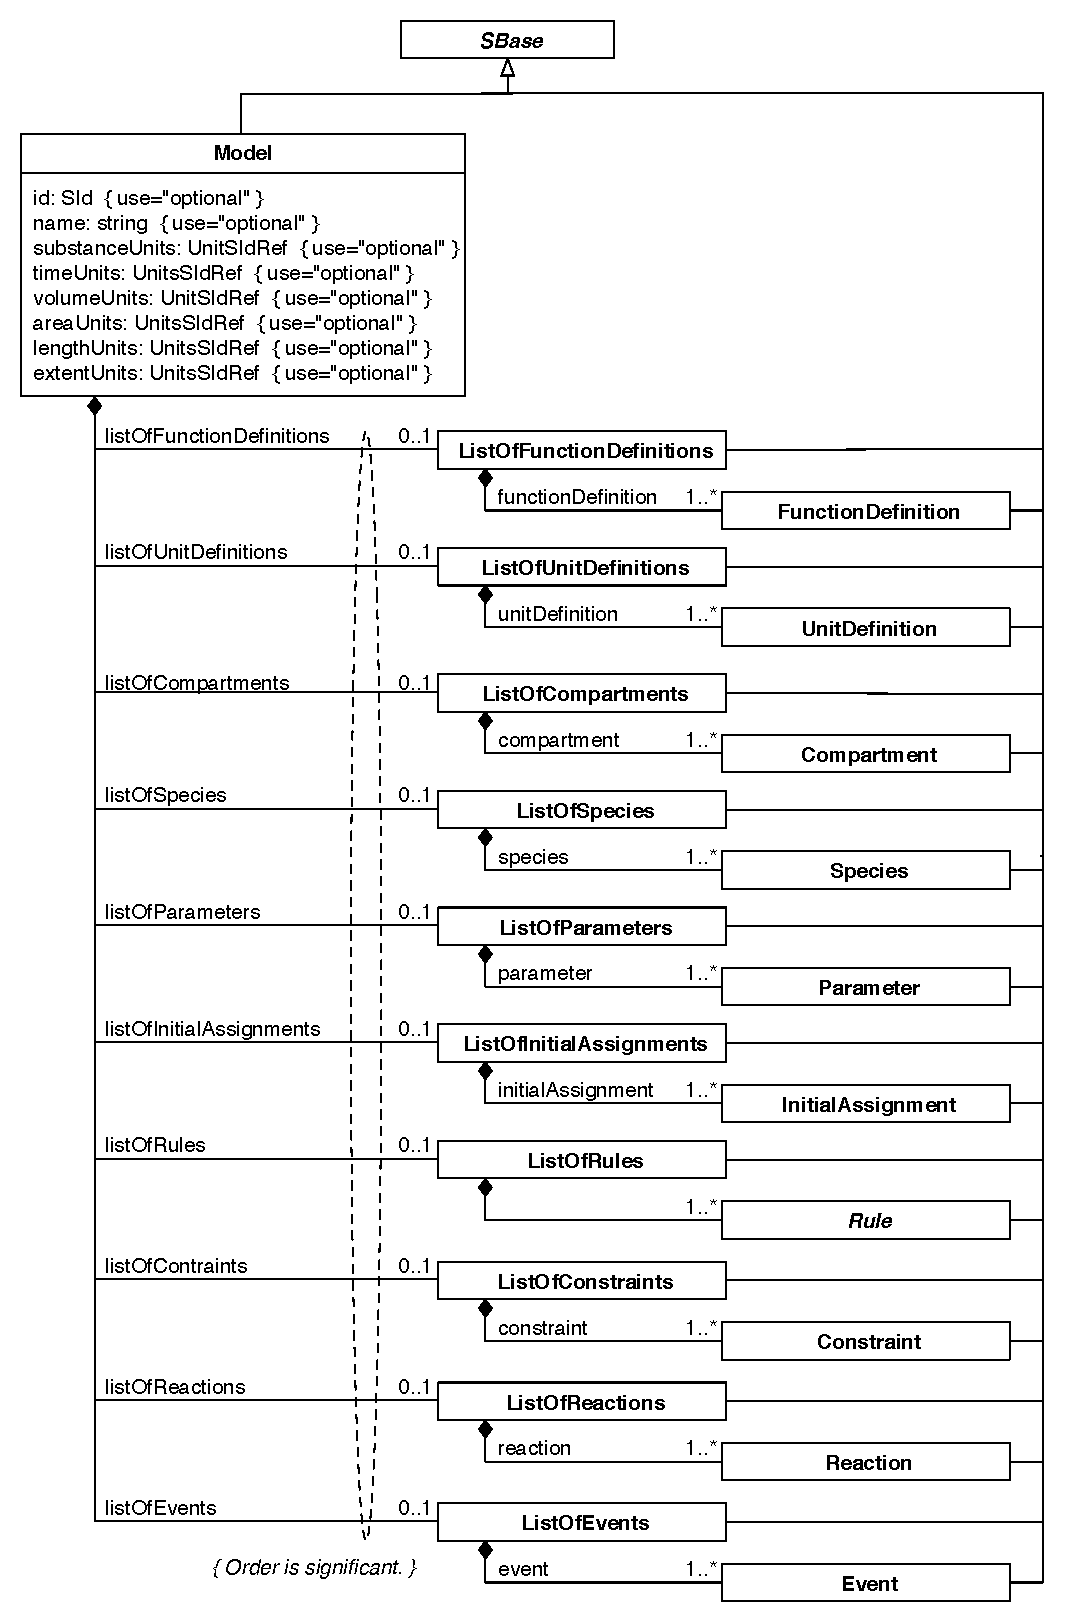
\includegraphics[scale=0.75]{figs/model-uml}
  \caption{The definition of \Model and the many helper
      classes \ListOfFunctionDefinitions, \ListOfUnitDefinitions,
      \ListOfCompartments, \ListOfSpecies, \ListOfParameters,
      \ListOfInitialAssignments, \ListOfRules, \ListOfConstraints,
      \ListOfReactions, and \ListOfEvents.}
  \label{fig:model}
\end{figure}

\Model serves as a container for components of classes
\FunctionDefinition, \UnitDefinition, \Compartment, \Species, \Parameter,
\InitialAssignment, \Rule, \Constraint, \Reaction and \Event.
Instances of the classes are placed inside instances of classes
\ListOfFunctionDefinitions, \ListOfUnitDefinitions,
\ListOfCompartments, \ListOfSpecies, \ListOfParameters, \ListOfInitialAssignments,
\ListOfRules, \ListOfConstraints, \ListOfReactions, and
\ListOfEvents.  The ``list'' classes are defined in
Figure~\ref{fig:model}.  All of the lists are optional, but if a
given list container is present within the model, the list must
not be empty; that is, it must have length one or more.  The
resulting XML data object for a full model containing every
possible list would have the following form:

\newcommand{\sayOptional}{\raisebox{0pt}[0pt][0pt]{\bigg\} \textrm{\emph{optional}}}}

\vspace*{2ex}
\begin{tt}
  \tightspacing
  \small
  \begin{tabbing}
xxxx\=xxxx\=xxxx\=xxxx\=xxxx\=\kill
\+\>
<?xml version="1.0" encoding="UTF-8"?>\\
<sbml xmlns="http://www.sbml.org/sbml/level3/version1/core" level="3" version="1">\\
\><model id="My\_Model">\\
\>\><listOfFunctionDefinitions>\\
\>\>\>\textrm{\emph{one or more}} <functionDefinition> ... </functionDefinition> \textrm{\emph{elements}}  \` \sayOptional\\
\>\></listOfFunctionDefinitions>\\
\>\><listOfUnitDefinitions>\\
\>\>\>\textrm{\emph{one or more}} <unitDefinition> ... </unitDefinition> \textrm{\emph{elements}}  \` \sayOptional\\
\>\></listOfUnitDefinitions>\\
\>\><listOfCompartments>\\
\>\>\>\textrm{\emph{one or more}} <compartment> ... </compartment> \textrm{\emph{elements}}  \` \sayOptional\\
\>\></listOfCompartments>\\
\>\><listOfSpecies>\\
\>\>\>\textrm{\emph{one or more}} <species> ... </species> \textrm{\emph{elements}}  \` \sayOptional\\
\>\></listOfSpecies>\\
\>\><listOfParameters>\\
\>\>\>\textrm{\emph{one or more}} <parameter> ... </parameter> \textrm{\emph{elements}}  \` \sayOptional\\
\>\></listOfParameters>\\
\>\><listOfInitialAssignments>\\
\>\>\>\textrm{\emph{one or more}} <initialAssignment> ... </initialAssignment> \textrm{\emph{elements}}  \` \sayOptional\\
\>\></listOfInitialAssignments>\\
\>\><listOfRules>\\
\>\>\>\textrm{\emph{one or more elements of subclasses of \abstractclass{Rule}}}  \` \sayOptional\\
\>\></listOfRules>\\
\>\><listOfConstraints>\\
\>\>\>\textrm{\emph{one or more}} <constraint> ... </constraint> \textrm{\emph{elements}}  \` \sayOptional\\
\>\></listOfConstraints>\\
\>\><listOfReactions>\\
\>\>\>\textrm{\emph{one or more}} <reaction> ... </reaction> \textrm{\emph{elements}}  \` \sayOptional\\
\>\></listOfReactions>\\
\>\><listOfEvents>\\
\>\>\>\textrm{\emph{one or more}} <event> ... </event> \textrm{\emph{elements}}  \` \sayOptional\\
\>\></listOfEvents>\\
\></model>\\
</sbml>
\end{tabbing}
\regularspacing
\end{tt}
\vspace*{0.5ex}

Although the lists are optional, there are dependencies between
SBML components such that defining some components requires
defining others.  For example, defining a species requires
defining a compartment, and defining a reaction requires defining
a species.  Such dependencies are explained throughout this
document.
  

\subsubsection{The \token{id} and \token{name} attributes}
\label{sec:model-id}

The \Model object has an optional attribute, \token{id}, used to
give the model an identifier.  The value of \token{id} must
conform to the syntax permitted by the \primtype{SId} data type
described in Section~\ref{sec:sid}.  \Model also has an optional
\token{name} attribute, of type \primtype{string}.  The
\token{name} and \token{id} attributes must be used as described
in Section~\ref{sec:idnameattribs}.


\subsubsection{The \token{sboTerm} attribute}
\label{sec:model-sboterm}

\Model inherits an optional \token{sboTerm} attribute of type
\primtype{SBOTerm} from its parent class \SBase (see
Sections~\ref{sec:sboterm-type} and~\ref{sec:sboTerm}).  When a
value is given to this attribute in a \Model instance, it should
be an SBO identifier belonging to the branch for type \Model
indicated in Table~\ref{tab:sboterm-availability}.  The
  relationship is of the form ``the model definition \emph{is-a}
  X'', where X is the SBO term.  The term chosen should be the
most precise (narrow) one that captures the overall process or
phenomenon represented by the overall SBML model.

As discussed in Section~\ref{sec:sboTerm}, SBO labels are optional
information on a model.  Applications are free to ignore
\token{sboTerm} values.  A model must be interpretable without the
benefit of SBO labels.


\subsubsection{The \token{substanceUnits} attribute}
\label{sec:model-substanceUnits}
\label{sec:substanceunits}

The \token{substanceUnits} attribute is used to specify the unit
of measurement associated with substance quantities of \Species
objects that do not specify units explicitly.  The attribute's
value must be of type \primtype{UnitSIdRef}
(Section~\ref{sec:unitsidref}).  A list of recommended units is
given in Section~\ref{sec:bp:unitdefinitions:recommendedunits}.

If a given \Species object definition does not specify its unit of
substance quantity via the \token{substanceUnits} attribute on
\Species (described in Section~\ref{sec:species}), then the
species inherits the value of the \Model \token{substanceUnits}
attribute.  If the \Model does not define a value for this
attribute, then there is no unit to inherit, and all species that
do not specify individual \token{substanceUnits} attribute values
then have \emph{no} declared units for their quantities.
Section~\ref{sec:species-substanceunits} provides more information
about the units of species quantities.

Note that when the identifier of a species appears in a model's
mathematical expressions, the unit of measurement associated with
that identifier is \emph{not solely determined} by setting
\token{substanceUnits} on \Model or \Species.
Sections~\ref{sec:species-units} and~\ref{sec:species-meaning}
explain this point in more detail.


\subsubsection{The \token{timeUnits} attribute}
\label{sec:model-timeUnits}
\label{sec:timeunits}

The \token{timeUnits} attribute is used to specify the unit in
which time is measured in the model.  The value of this attribute
must be of type \primtype{UnitSIdRef}
(Section~\ref{sec:unitsidref}).  A list of recommended units is
given in Section~\ref{sec:bp:unitdefinitions:recommendedunits}.

This attribute on \Model is the \emph{only} way to specify a unit
for time in a model.  It is a global attribute; time is measured
in the model everywhere in the same way.  This is particularly
relevant to \Reaction and \RateRule objects in a model: all
\Reaction and \RateRule objects in SBML define per-time values,
and the unit of time is given by the \token{timeUnits} attribute
on the \Model object instance.  If the \Model \token{timeUnits}
attribute has no value, it means that the unit of time is not
defined for the model's reactions and rate rules.  Leaving it
unspecified in an SBML model does not result in an invalid model;
however, as a matter of best practice, we strongly recommend that
all models specify units of measurement for time.


\subsubsection{The \token{volumeUnits}, \token{areaUnits} and
  \token{lengthUnits} attributes}
\label{sec:model-volumeUnits}
\label{sec:model-areaUnits}
\label{sec:model-lengthUnits}
\label{volumeunits}
\label{areaunits}
\label{lengthunits}

The attributes \token{volumeUnits}, \token{areaUnits} and
\token{lengthUnits} together are used to set the units of
measurements for the sizes of \Compartment objects in the model
when those objects do not otherwise specify units.  The three
attributes correspond to the most common cases of compartment
dimensions: \token{volumeUnits} for compartments having attribute
value \token{spatialDimensions}=\val{3}, \token{areaUnits} for
compartments having \token{spatialDimensions}=\val{2}, and
\token{lengthUnits} for compartments having
\token{spatialDimensions}=\val{1}.  The values of these attributes
must be of type \primtype{UnitSIdRef}
(Section~\ref{sec:unitsidref}).  A list of recommended units is
given in Section~\ref{sec:bp:unitdefinitions:recommendedunits}.
The attributes are not applicable to compartments whose
\token{spatialDimensions} attribute values are not one of \val{1},
\val{2} or \val{3}.

If a given \Compartment object instance does not provide a value
for its \token{units} attribute, then the unit of measurement of
that compartment's size is inherited from the value specified by
the \Model \token{volumeUnits}, \token{areaUnits} or
\token{lengthUnits} attribute, as appropriate based on the
\Compartment object's \token{spatialDimensions} attribute value.
If the \Model object does not define the relevant attribute, then
there are no units to inherit, and all compartments that do not
set a value for their \token{units} attribute then have \emph{no}
units associated with their compartment sizes.
Section~\ref{sec:compartment-units} provides more information
about units of compartment sizes.

The use of three separate attributes is a carry-over from SBML
Level~2.  Note that it is entirely possible for a model to define
a value for two or more of the attributes \token{volumeUnits},
\token{areaUnits} and \token{lengthUnits} simultaneously, because
SBML models may contain compartments with different numbers of
dimensions.


\subsubsection{The \token{extentUnits} attribute}
\label{sec:model-extentUnits}
\label{extentunits}

Reactions are processes that occur over time.  These processes
involve events of some sort, where a single ``reaction event'' is
one in which some set of entities (known as reactants, products
and modifiers in SBML) interact, once.  The \emph{extent} of a
reaction is a measure of how many times the reaction has occurred,
while the time derivative of the extent gives the instantaneous
rate at which the reaction is occurring.  Thus, what is
colloquially referred to as the ``rate of the reaction'' is in
fact equal to the rate of change of reaction extent.

The combination of \token{extentUnits} and \token{timeUnits}
defines the units of kinetic laws in SBML and establishes how the
numerical value of each \KineticLaw's mathematical formula
(Section~\ref{subsec:kinetic-law}) is meant to be interpreted in a
model.  The units of the kinetic laws are taken to be
\token{extentUnits} divided by \token{timeUnits}.  A list of
recommended units is given in
Section~\ref{sec:bp:unitdefinitions:recommendedunits}.

Note that this embodies an important principle in SBML models:
\emph{all reactions in an SBML model must have the same units} for
the rate of change of extent.  In other words, the units of all
reaction rates in the model \emph{must be the same}.  There is
only one global value for \token{extentUnits} and one global value
for \token{timeUnits}.


\subsubsection{The \token{conversionFactor} attribute}
\label{sec:model-conversionFactor}

The attribute \token{conversionFactor} defines a global value
inherited by all \Species object instances that do not define
separate values for their \token{conversionFactor} attributes.  The
value of this attribute must be of type \primtype{SIdRef}
(Section~\ref{sec:sidref}) and refer to a \Parameter object
instance defined in the model.  The \Parameter object in question
must be a constant; \ie it must have its \token{constant}
attribute value set to \val{true}.

If a given \Species object definition does not specify a
conversion factor via the \token{conversionFactor} attribute on
\Species (described in Section~\ref{sec:species}), then the
species inherits the conversion factor specified by the \Model
\token{conversionFactor} attribute.  If the \Model does not define
a value for this attribute, then there is no conversion factor to
inherit.  Section~\ref{sec:about-kinetic-laws} describes how to
interpret the effects of reactions on species in that situation.
More information about conversion factors in SBML is provided in
Sections~\ref{sec:species} and~\ref{sec:reactions}.


\subsubsection{The ListOf container classes}
\label{sec:listof}
\label{sec:listofunitdefinitions}
\label{sec:listoffunctiondefinitions}
\label{sec:listofcompartments}
\label{sec:listofspecies}
\label{sec:listofparameters}
\label{sec:listofinitialassignments}
\label{sec:listofinitialassign}
\label{sec:listofrules}
\label{sec:listofconstraints}
\label{sec:listofreactions}
\label{sec:listofevents}

The various \ListOf classes defined in Figure~\ref{fig:model} are
merely containers used for organizing the main components of an
SBML document.  \ListOfFunctionDefinitions,
\ListOfUnitDefinitions, \ListOfCompartments, \ListOfSpecies,
\ListOfParameters, \ListOfInitialAssignments, \ListOfRules,
\ListOfConstraints, \ListOfReactions, and \ListOfEvents are all
derived from the abstract class \SBase (Section~\ref{sec:sbase}),
and inherit \SBase's various attributes and subelements.  The
\ListOf classes do not add any attributes of their own.

There are several motivations for grouping SBML components within
XML elements with names of the form \token{listOfClassNames}
rather than placing all the components directly at the top level.
First, the fact that the container classes are derived from \SBase
means that software tools can add information about the lists
themselves into each list container's \Annotation, a feature that
a number of today's software tools exploit.  Second, we believe
the grouping leads to a more modular structure that is helpful
when working with elements from multiple SBML Level~3 packages.
Third, we believe that it makes visual reading of models in XML
easier, for situations when humans must inspect and edit SBML
directly.


%-----------------------------------------------------------------------------
\subsection{Function definitions}
\label{sec:functiondefinition}
%-----------------------------------------------------------------------------

The \FunctionDefinition object associates an identifier with a
function definition.  This identifier can then be used as the
function called in subsequent MathML \token{apply} elements.
\FunctionDefinition is shown in Figure~\ref{fig:mathdefinition}.

\begin{figure}[htb]
  \centering
  \small
  \vspace*{-0.75ex}
  \begin{tikzpicture}
    \node[above=0.4in] (a) {
      \emptyClassbox{\textsl{SBase}}
    };
    \node (b) {
      \begin{classbox}{\textcolor{black}{FunctionDefinition}}
        id: SId                           \\
        name: string \{ use="optional" \} \\
      \end{classbox}
    };
    \node[right=1.6in] (c) {
      \begin{classbox}{Lambda}
        xmlns: string \{ "http://www.w3.org/1998/Math/MathML" \} \\
        \{ \emph{\mathml content restricted to one \mathml \token{lambda}} \\[-1pt]
        \emph{or one \token{semantics} element containing a \token{lambda}. \}} \\
      \end{classbox}
    };
    \draw[open triangle 60-] (a) -- (b);
    \draw[diamond-,shorten <=-3pt,shorten >=-6pt] (b) -- (c)
        node[above=6pt,left=1.8in] {\textsf{math}};
  \end{tikzpicture}
  \vspace*{-2ex}
  \caption{The definition of class \FunctionDefinition.  A
    \class{Lambda} class object must contain a single \mathml
    \token{lambda} expression (or a \token{lambda} surrounded by a
    \token{semantics} element).  A function definition must
    contain exactly one \token{math} element defined by the
    \class{Lambda} class.  Note also that \class{Lambda} is not
    derived from \SBaseUpright, which means that the attributes defined
    on \SBaseUpright are \emph{not} available on the \token{math}
    element.  A sequence of one or more instances of
    \FunctionDefinition objects can be located in an instance of
    \ListOfFunctionDefinitions in \Model, as shown in
    Figure~\protect\ref{fig:model}.}
  \label{fig:mathdefinition}
  \label{fig:functionDefinition}
\end{figure}

Function definitions in SBML (also informally known as
``user-defined functions'') have purposefully limited capabilities.
As is made clearer below, a function cannot reference
parameters or other model quantities outside of itself; values
must be passed as parameters to the function.  Moreover, recursive
and mutually-recursive functions are not permitted.  The purpose
of these limitations is to balance power against complexity of
implementation.  With the restrictions as they are, function
definitions could, if desired, be implemented as textual substitutions.
Software implementations therefore do not need
the full function-definition machinery typically associated with
programming languages.


\subsubsection{The \token{id} and \token{name} attributes}

The \token{id} and \token{name} attributes have types \primtype{SId}
and \primtype{string}, respectively, and operate in the manner
described in Section~\ref{sec:idnameattribs}.  MathML \token{ci}
elements in an SBML model can refer to the function defined by a
\FunctionDefinition using the value of its \token{id} attribute.


\subsubsection{The \token{math} element}
\label{sec:function-definition-math}

The \token{math} element is a container for MathML content that
defines the function.  The content of this element can only be a
MathML \token{lambda} element or a MathML \token{semantics}
element containing a \token{lambda} element.  \FunctionDefinition
is the only place in SBML Level~3 Core where a \token{lambda}
element can be used.  The \token{lambda} element must begin with
zero or more \token{bvar} elements, followed by any other of the
elements in the MathML subset listed in
Section~\ref{sec:mathmlsubset} \emph{except} \token{lambda} (\ie a
\token{lambda} element cannot contain another \token{lambda}
element).

A further restriction on the content of \token{math} is it cannot
contain references to identifiers other than the
variables declared in the \token{lambda} itself.  That
is, the contents of MathML \token{ci} elements inside the body of
the \token{lambda} can only be one of two kinds of
  identifiers: (i) the variables declared by its \token{bvar}
  elements, or (ii) the identifiers of other
\FunctionDefinition{} objects defined in the same model.  This
restriction also applies to the \token{csymbol} elements for
\quantity{time}, \quantity{avogadro} and \quantity{delay}.
Functions must be written so that all model variables they use are
passed to them via their parameters.


\subsubsection{The \token{sboTerm} attribute}
\label{sec:functiondefinition-sboterm}

\FunctionDefinition inherits an optional \token{sboTerm}
attribute of type \primtype{SBOTerm} from its parent
class \SBase (see Sections~\ref{sec:sboterm-type}
and~\ref{sec:sboTerm}).  When a value is given to this
attribute in a \FunctionDefinition instance, it should be an
SBO identifier belonging to the branch for type \FunctionDefinition 
indicated in Table~\ref{tab:sboterm-availability}.  The relationship is
of the form ``the function definition \emph{is-a} X'', where X is
the SBO term.  The term chosen should be the most precise (narrow)
one that captures the role of the function in the model.

As discussed in Section~\ref{sec:sboTerm}, SBO labels are optional
information on a model.  Applications are free to ignore
\token{sboTerm} values.  A model must be interpretable without the
benefit of SBO labels.


\subsubsection{Calling user-defined functions}
\label{sec:functiondefinition-calling}

Within MathML expressions in an SBML model, all calls to a
function defined by a \FunctionDefinition must use the same number
of arguments as specified in the function's definition.  The
number of arguments is equal to the number of \token{bvar}
elements inside the \token{lambda} element of the function
definition.

Note that \FunctionDefinition does not have a separate attribute
for defining the unit of measurement associated with the value
returned by the function.  The unit is taken to be whatever
results from evaluating the expression when the
\FunctionDefinition's \token{math} is applied to the arguments
supplied in the call to that function.  (See also
Section~\ref{sec:unit-consistency}.)


\subsubsection{Examples}

The following abbreviated SBML example shows a \FunctionDefinition
object instance defining \token{pow3} as the identifier of a function
computing the mathematical expression $x^{3}$, and after that, the
invocation of that function in the mathematical formula of a rate
law.  Note how the invocation of the function uses its identifier.

\begin{example}
<model ...>
   <listOfFunctionDefinitions>
       <functionDefinition id="pow3">
           <math xmlns="http://www.w3.org/1998/Math/MathML"
                 xmlns:sbml="http://www.sbml.org/sbml/level3/version1/core">
               <lambda>
                   <bvar><ci> x </ci></bvar>
                   <apply> <power/> <ci> x </ci> <cn sbml:units="dimensionless"> 3 </cn> </apply>
               </lambda>
           </math>
       </functionDefinition>
   </listOfFunctionDefinitions>
   ...
   <listOfReactions>
       <reaction id="reaction_1" reversible="true" fast="false">
           ...
           <kineticLaw>
               <math xmlns="http://www.w3.org/1998/Math/MathML">
                   <apply> <ci> pow3 </ci> <ci> S1 </ci> </apply>
               </math>
           </kineticLaw>
           ...
       </reaction>
   </listOfReactions>
   ...
</model>\end{example}


%-----------------------------------------------------------------------------
\subsection{Unit definitions}
\label{sec:unitdefinitions}
%-----------------------------------------------------------------------------

The unit of measurement associated with the value produced by a
mathematical formula is whatever arises naturally from the
components and mathematical expressions comprising the formula, or
in other words, the unit obtained by doing dimensional analysis on
the formula.  To support this, units may be supplied in a number
of contexts in an SBML model and associated with a variety of
components, and SBML provides a facility for defining units that
can be reused and referenced throughout a model.  The unit
definition facility uses two classes of objects, \UnitDefinition
and \Unit.  Their definitions are shown in
Figure~\vref{fig:unitdefinition} and explained in more detail
below.

Before delving further into the definition of SBML units, we must
highlight two important and sometimes-confusing points.  First,
unit declarations in SBML models are \emph{optional}.  The
consequence of this is that a model must be numerically
self-consistent independently of unit declarations, for the
benefit of software tools that cannot interpret or manipulate
units.  Unit declarations in SBML are thus more akin to a type of
annotation; they can indicate intentions, and can be used by model
readers for checking the consistency of the model, labeling
simulation output, etc., but any transformations of values implied
by different units must be incorporated \emph{explicitly} into a
model.  We revisit this topic in Section~\ref{sec:using-units},
and illustrate it again with the example given in
Section~\ref{sec:eg:conversionfactor}.

Second, the vast majority of situations that require new SBML unit
definitions involve simple multiplicative combinations of base
units and factors.  An example is ``moles per litre per second''.
What distinguishes these sorts of unit definitions from more
complex ones is that they may be expressed without the use of an
additive offset from a zero point.  The use of offsets complicates
all unit definition systems, yet in the domain of SBML, the
real-life cases requiring offsets are few (and in fact, to the
best of our knowledge, only involve temperature).  Consequently,
the SBML unit system has been consciously designed to simplify
implementation of unit support for the most common cases in
systems biology.  The cost of this simplification is to require
units with offsets to be handled explicitly by the modeler.
Section~\ref{sec:bp:unitdefinitions:offset} discusses approaches
for handling situations requiring units with offsets.


\subsubsection{\class{UnitDefinition}}
\label{sec:unitdefinition-structure}

The approach to defining units in SBML is compositional; for
example, $metre\ second^{\,-2}$ is constructed by combining a
\Unit object representing $metre$ with another \Unit object
representing $second^{\,-2}$.  The combination is wrapped inside a
\UnitDefinition, which provides for assigning an identifier and
optional name to the combination.  These object classes are
defined in Figure~\ref{fig:unitdefinition}.  Once a unit is
defined using a \UnitDefinition object, it can then be referenced
from elsewhere in a model.

\begin{figure}[htb]
  \centering
  \vspace*{1ex}
  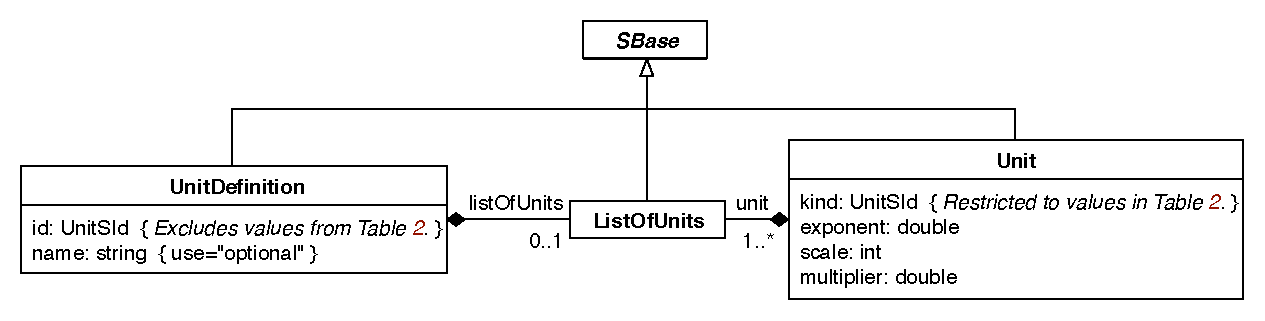
\includegraphics[scale=0.78]{figs/unitdefinition-uml}
  \caption{The definition of classes \UnitDefinition and
      \Unit.  A sequence of one or more instances of
      \UnitDefinition can be located in an instance of
      \ListOfUnitDefinitions in \Model
      (Figure~\protect\ref{fig:model}).  \ListOfUnits has
      no attributes (beyond those it inherits from class \SBaseUpright);
      it merely acts as a container for one or more instances of
      \Unit objects.  Note that the only permitted values of
      \token{kind} on \Unit are the reserved words in
      Table~\vref{tab:unitkind}, but these symbols are
      \emph{excluded} from the permitted values of
      \UnitDefinition's \token{id} because SBML's unit system does
      not allow redefining the base units.}
  \label{fig:unitdefinition}
\end{figure}


\paragraph{The \token{id} and \token{name} attributes}

The required attribute \token{id} and optional attribute
\token{name} have data types \primtype{UnitSIdRef}
(Section~\ref{sec:unitsidref}) and \primtype{string},
respectively.  The \token{id} attribute is used to give the
defined unit a unique identifier by which other parts of the model
may refer to the unit.  The \token{name} attribute is intended to
be used for giving the unit definition an optional human-readable
name; see Section~\ref{sec:name} for more guidelines about the use
of names.

There is one important restriction about the use of unit
definition \token{id} values: the \token{id} of a \UnitDefinition
must \emph{not} be equal to one of the reserved base unit
  names listed in Table~\ref{tab:unitkind}, the list of reserved
base unit names.  This constraint simply prevents the redefinition
of base units.


\paragraph{The list of \class{Unit}s}
\label{sec:listofunits}

A \UnitDefinition object may contain a \ListOfUnits container which must
contain one or more \Unit objects. Section~\ref{sec:unit-structure} explains
the meaning and use of \Unit.   

\paragraph{Example}

The following skeleton of a unit definition illustrates an example
use of \UnitDefinition:

\begin{example}
<model ...>
    <listOfUnitDefinitions>
        <unitDefinition id="unit1">
            <listOfUnits>
                ...
            </listOfUnits>
        </unitDefinition>
        <unitDefinition id="unit2">
            <listOfUnits>
                ...
            </listOfUnits>
        </unitDefinition>
    </listOfUnitDefinitions>
    ...
</model>
\end{example}


\subsubsection{\class{Unit}}
\label{sec:unit-structure}

A \Unit object represents a reference to a (possibly transformed)
base unit chosen from the list in Table~\vref{tab:unitkind}.  The
attribute \token{kind} indicates the base unit, whereas the
attributes \token{exponent}, \token{scale}, and \token{multiplier}
define how the base unit is being transformed.  The attributes
are described in detail below.


\paragraph{The \token{kind} attribute}

The \Unit attribute \token{kind} specifies a base unit to serve as
the starting point for a new unit definition.  The value of the
attribute must be taken from the list of reserved words given in
Table~\vref{tab:unitkind}.  These reserved symbols are defined in
the value space of the data type \primtype{UnitSId}
(Section~\ref{sec:unitsid}).

\begin{table}[bht]
  \vspace*{1em}
  \centering
  \ttfamily
  \small
  \setlength{\arraycolsep}{8pt}
  \begin{edtable}{tabular}{@{}llllll@{}}
    \toprule
    ampere                    & farad            & joule    & lux      & radian    & volt  \\
    \underline{avogadro}      & gram             & katal    & metre    & second    & watt  \\
    becquerel                 & gray             & kelvin   & mole     & siemens   & weber \\
    candela                   & henry            & kilogram & newton   & sievert           \\
    coulomb                   & hertz            & litre    & ohm      & steradian         \\
    \underline{dimensionless} & \underline{item} & lumen    & pascal   & tesla             \\
    \bottomrule
  \end{edtable}
  \caption{Base units defined in SBML.  These symbols are
    predefined values of type \primtype{UnitSId}
    (Section~\ref{sec:unitsid}).  All are names of base or derived
    SI units~\protect\citep{bipm:2006}, except for
    ``\token{avogadro}'', ``\token{dimensionless}'' and
    ``\token{item}'', which are SBML additions.  The unit
    ``\token{dimensionless}'' is intended for cases where a
    quantity is a ratio whose units cancel out, the unit
    ``\token{avogadro}'' is the unit ``\token{dimensionless}''
    multiplied with Avogadro's number, 
    and ``\token{item}'' is used for expressing such things as 
    ``N items'' when ``mole'' is not an appropriate unit.   The
    gram and litre are not strictly part of SI; however, they are
    frequently used in SBML's areas of application and therefore
    are included as predefined unit identifiers.  (The standard SI
    unit of mass is the kilogram, and  volume in SI is defined in
    terms of cubic metres.)  Comparisons of these values, like all
    values of type \primtype{UnitSId}, must be performed in a
    case-sensitive manner.}
  \label{tab:unitkind}
\end{table}

Note that the set of acceptable values for the attribute
\token{kind} does \emph{not} include units defined by
\UnitDefinition objects.  This means that the unit definition
system in SBML is not hierarchical: user-defined units cannot be
built on top of other user-defined units, only on top of base
units.

The presence of \token{avogadro} in Table~\ref{tab:unitkind}
warrants an explanation.  The Bureau International des Poids et
Mesures specifically states, ``When the mole is used, the
elementary entities must be specified and may be atoms, molecules,
ions, electrons, other particles, or specified groups of such
particles''~\cite[p.~115]{bipm:2006}---in other words, the SI unit
\token{mole} is technically \emph{a unit of measure for substance
  amount}.  Although people sometimes use ``mole'' loosely to
refer to other things besides substance amounts (\eg ``a mole of
\emph{X}'' to mean a number of \emph{X} equal to Avogadro's
number, $6.022 \cdot 10^{23}$), such usage is not strictly
correct.  We believe it is even less correct in the context of
reactions: although in SBML they are called ``reactions'', there
is nothing preventing the SBML \Reaction construct from being used
to represent other kinds of processes not involving substances.
Consequently, we avoid using \val{mole} loosely where substances
may not be involved, and instead use ``Avogadro's number of
\emph{X}''.  In order to make it easier for models to define units
in these terms, the SBML unit system includes the pseudo-unit
\val{avogadro}, whose definition is identical to the definition of
the \emph{avogadro} \token{csymbol} described in
Section~\ref{sec:csymbol}.  The numerical value is taken to be the
one recommended by CODATA~\citep{codata_2008}, but the unit is
\token{dimensionless}.  In other words, it is defined as
\begin{linenomath}
  \begin{equation*}
    (6.02214179 \cdot 10^{23}) \cdot \texttt{dimensionless}
  \end{equation*}
\end{linenomath}
where the dot ($\cdot$) indicates simple scalar multiplication.
If the value of Avogadro's constant is revised by international
standards-setting organizations in the future, a future Version of
the SBML \thisL specification may stipulate a new value to be used
for \token{avogadro}.  However, all software reading models
expressed in \emph{this} version of SBML Level~3 should
\emph{always} use the value of Avogadro's constant given above.

Software tools must use identical numerical values of Avogadro's
constant for both the base unit \token{mole} and the unit \token{avogadro}.


\paragraph{The \token{exponent}, \token{scale} and
  \token{multiplier} attributes}
\label{sec:unit-structure:exponent}
\label{sec:unit-structure:scale}
\label{sec:unit-structure:multiplier}

\newcommand{\ynew}{\ensuremath{y}\xspace}
\newcommand{\ybase}{\ensuremath{y_b}\xspace}
\newcommand{\udef}{\ensuremath{u}\xspace}
\newcommand{\unew}{\ensuremath{u_\text{new}}\xspace}
\newcommand{\ubase}{\ensuremath{u_b}\xspace}
\newcommand{\ukind}{\ensuremath{u_\token{\,kind}}\xspace}
\newcommand{\uone}{\ensuremath{u_{b_1}}\xspace}
\newcommand{\utwo}{\ensuremath{u_{b_2}}\xspace}
\newcommand{\un}  {\ensuremath{u_{b_n}}\xspace}

The attributes \token{exponent}, \token{scale} and
\token{multiplier} work together to permit the use of \Unit for
expressing new units in terms of the base units listed in
Table~\vref{tab:unitkind}.  The formula underlying this definition
is the following:
\begin{linenomath}
\begin{equation}
  \unew = (\token{multiplier} \cdot 10^\token{scale} \cdot \ukind)^\token{exponent}
\label{eq:unit-semantics}
\end{equation}
\end{linenomath}

This formula defines a new unit, \unew, in terms of another unit,
\ukind.  The unit \ukind is one of the units listed in
Table~\ref{tab:unitkind}; in a given \Unit object, it is
chosen by setting the \token{kind} attribute.  Each of the other
components on the right-hand side of
Equation~\ref{eq:unit-semantics} corresponds to the remaining
attributes in a \Unit object instance, and their meanings are as
follows:
\begin{itemize}

\item The \token{multiplier} attribute can be used to multiply the
  \token{kind} unit by a real-numbered factor.  This enables the
  definition of units that are not power-of-ten multiples of SI
  units.  For instance, a \token{multiplier} of 0.3048 could be
  used to define \val{foot} as a measure of length in terms of a
  \val{metre}.  A value of \token{multiplier} must always be
  provided in a \Unit object instance, but the value can be
  \val{1}.

\item The \token{scale} attribute can be used to set the exponent
  for a power-of-ten multiplier that rescales the unit.  For
  example, a unit having a \token{kind} value of \val{gram} and a
  \token{scale} value of \val{-3} signifies $10^{-3} \cdot gram$,
  or milligrams.  In those cases where a unit does not need to be
  scaled by a power of ten, the value of \token{scale} can be set
  to \val{0} (zero), because $10^0 = 1$.

\item The \token{exponent} attribute can be used to specify an
  overall exponent on the unit definition.  This provides a way to
  define units such as ``cubic metre'' in terms of the base unit
  \val{metre} (for which an \token{exponent} value of~\val{3}
  would be appropriate).  A value of \token{exponent} must always
  be provided.

\end{itemize}


\subsubsection{Semantics of \class{Unit} and \class{UnitDefinition}}
\label{sec:unit-structure:semantics}

A single \Unit object instance takes one of the base units from
Table~\ref{tab:unitkind} and specifies how it should be
transformed.  A \UnitDefinition object instance combines one or
more \Unit objects to define a new, composed unit, \udef.  The new
unit \udef created by a \UnitDefinition is defined as the product
of all the \Unit objects contained in the \ListOfUnits within the
\UnitDefinition object instance.  More formally, 
\begin{linenomath}
\begin{equation}
  \udef = u_1 \, \cdot \, u_2 \, \cdot \ldots \cdot \, u_n 
\label{eq:unitDefinition-semantics}
\end{equation}
\end{linenomath}
where the $\{u_i\}$'s are individual \Unit definitions as defined
by Equation~\ref{eq:unit-semantics}.  Now, let the value of the
\token{multiplier} attribute of a given unit $\{u_i\}$ be
represented by the variable $m_i$.  Similarly, let the value of
the \token{scale} attribute be represented by $s_i$, and the value
of the \token{exponent} attribute be represented by $x_i$.
Equation~\ref{eq:unitDefinition-semantics} can be rewritten in
expanded form as
\begin{linenomath}
\begin{align}
  u &= (m_1 \cdot 10^{s_1} \cdot \uone)^{x_1} \cdot
       (m_2 \cdot 10^{s_2} \cdot \utwo)^{x_2} \cdot \ldots \cdot (m_n \cdot
       10^{s_n} \cdot \un)^{x_n} \notag \\[2pt]
    &= m_1^{x_1} \cdot m_2^{x_2} \cdot \ldots \cdot m_n^{x_n}
       \cdot 10^{(s_1 x_1 + s_2 x_2 + \ldots + s_n x_n)}
       \cdot \uone^{x_1} \cdot \utwo^{x_2} \cdot \ldots \cdot \un^{x_n} \notag \\[2pt]
    &= m \cdot 10^{s} \cdot \uone^{x_1} \cdot \utwo^{x_2} \cdot \ldots \cdot \un^{x_n}
\label{eq:multip-units}
\end{align}
\end{linenomath}
where the terms $m$ and $s$ in the last line
(Equation~\ref{eq:multip-units}) are defined as
\begin{larray*}
  m &=& m_1^{x_1} \cdot m_2^{x_2} \cdot \ldots \cdot m_n^{x_n} \\
  s &=& s_1 x_1 + s_2 x_2 + \ldots + s_n x_n
\end{larray*}
Equation~\ref{eq:multip-units} expresses how a \UnitDefinition
object instance combines multiple \Unit object instances to
produce a new unit definition in an SBML model.


\paragraph{Examples}

As a concrete example to illustrate the definitions above, let us
define a unit for \val{foot} in terms of the base unit
\val{metre}.  This requires using \token{multiplier}=\val{0.3048},
\token{scale}=\val{0}, and \token{exponent}=\val{1}:
\begin{linenomath}
\begin{equation*}
  \text{foot} = 0.3048 \cdot 10^0 \cdot \token{metre}
\end{equation*}
\end{linenomath}
The following fragment of SBML illustrates how this could be
represented in XML:

\begin{example}
<listOfUnitDefinitions>
    <unitDefinition id="foot">
        <listOfUnits>
            <unit kind="metre" multiplier="0.3048" scale="0" exponent="1"/>
        </listOfUnits>
    </unitDefinition>
</listOfUnitDefinitions>
\end{example}

To give another example, the following illustrates the definition
of an abbreviation \val{mmls} for the unit $millimoles\ l^{-1}\
s^{-1}$:

\begin{example}
<listOfUnitDefinitions>
    <unitDefinition id="mmls">
        <listOfUnits>
            <unit kind="mole"   exponent="1"  scale="-3" multiplier="1"/>
            <unit kind="litre"  exponent="-1" scale="0"  multiplier="1"/>
            <unit kind="second" exponent="-1" scale="0"  multiplier="1"/>
        </listOfUnits>
    </unitDefinition>
</listOfUnitDefinitions>
\end{example}

Section~\ref{sec:bp:unitdefinitions:offset} provides suggestions
for possible ways of handling cases that involve offsets, which
happen in particular with temperature measurements.


\subsubsection{Use of units in a model}
\label{sec:using-units}

As already mentioned, unit declarations are optional in SBML.
This design decision was a consensus choice among SBML developers
and users, driven by the exigencies of non-commercial software
development and the realities of models found in existence.  It
has an important and possibly counterintuitive implication that
must be kept in mind when writing and interpreting SBML models:
units associated with quantities \emph{do not alter the numerical
  interpretation} of those quantities.

An example may help make this more clear.  We know that one metre
equals 1000 millimetres:
\begin{linenomath}
  \begin{equation*}
    1\, m = 1000\, mm
  \end{equation*}
\end{linenomath}
However, the equality above relies on interpreting the units on
both sides, and taking the ``1'' and ``1000'' to be dimensionless.
If readers ignored unit labels altogether or were unable to
process them, they would see
\begin{linenomath}
  \begin{equation*}
    1 = 1000
  \end{equation*}
\end{linenomath}
which is obviously incorrect.  In an SBML model, the necessary
factor must be included explicitly, even if it is part of the
definition of the unit.  A ramification of this is that units
attached to SBML quantities must be viewed as a kind of
independent annotation or label that does not enter into the
numerical interpretation of the actual quantity or the
mathematical formulas appearing in a model.  In the present simple
formula, an explicit factor such as the following needs to be
inserted (and here we put unit names in \{$\,$\} braces to
indicate they are annotations that do not enter into the
mathematics):
\begin{linenomath}
  \begin{equation}\label{eq:factor}
    1 \, \{m\} = 1000 \cdot \frac{1 \, \{m\}}{1000 \, \{mm\}} \, \{mm\}
  \end{equation}
\end{linenomath}
This is despite the fact that a unit definition for millimetres in SBML
would take the following form:
\begin{example}
<listOfUnitDefinitions>
    <unitDefinition id="millimetre">
        <listOfUnits>
            <unit kind="metre" exponent="1" scale="-3" multiplier="1"/>
        </listOfUnits>
    </unitDefinition>
</listOfUnitDefinitions>
\end{example}

In other words, the definition \emph{also} includes a factor of
$1/1000$.  While the result is that information is duplicated
between the definition of \token{millimetre} above and the
explicit factor inserted into Equation~\ref{eq:factor}, the
machinery provided by \UnitDefinition is still necessary in order
to allow units themselves to be properly defined.  The result is
still useful and powerful: it permits software tools to check the
consistency of a model, perform unit conversions, label numbers in
the outputs of simulations, and so on.


%-----------------------------------------------------------------------------
\subsection{Compartments}
\label{sec:compartments}
%-----------------------------------------------------------------------------

A \emph{compartment} in SBML represents a bounded space in which
species are located.  Compartments do not necessarily have to
correspond to actual structures inside or outside of a biological
system, although models are often designed that way.  The definition
of \Compartment is shown in Figure~\vref{fig:compartment}.

\begin{figure}[htb]
  \centering
  \small
  \begin{tikzpicture}
    \node[above=0.9in] (a) {
      \emptyClassbox{\textsl{SBase}}
    };
    \node (b) {
      \begin{classbox}{Compartment}
        id: SId \\
        name: string \{ use="optional" \} \\
        spatialDimensions: double \{ use="optional" \} \\
        size: double \{ use="optional" \} \\
        units: UnitSIdRef \{ use="optional" \} \\
        constant: boolean \\
      \end{classbox}
    };
    \draw[open triangle 60-] (a) -- (b);
  \end{tikzpicture}
  \caption{The definition of class \Compartment.  A
      sequence of one or more instances of \Compartment objects
      can be located in an instance of \ListOfCompartments in
      \Model, as shown in Figure~\protect\ref{fig:model}.}
  \label{fig:compartment}
\end{figure}

It is important to note that although compartments are optional in
the overall definition of \Model, every species in an SBML model
must be located in a compartment.  This in turn means that if a
model defines any species, the model must also define at least one
compartment.  The reason is simply that species represent physical
things, and therefore must exist \emph{somewhere}.  Compartments
represent the \emph{somewhere}.


\subsubsection{The \token{id} and \token{name} attributes}

\Compartment has one required attribute, \token{id}, of type
\primtype{SId}, to give the compartment a unique identifier by
which other parts of an SBML model definition can refer to it.  A
compartment can also have an optional \token{name} attribute of type
\primtype{string}.  Identifiers and names must be used according
to the guidelines described in Section~\ref{sec:idnameattribs}.


\subsubsection{The \token{spatialDimensions} attribute}
\label{sec:compartment-spatialdimensions}

A \Compartment object has an optional floating-point attribute
named \token{spatialDimensions} whose value indicates the number
of spatial dimensions possessed by the compartment.  Most modeling
scenarios involve compartments with integer values of
\token{spatialDimensions}=\val{3} (\ie a three-dimensional
compartment, which is to say, a volume),
\token{spatialDimensions}=\val{2} (\ie a two-dimensional
compartment, a surface), or \token{spatialDimensions}=\val{1} (\ie
a one-dimensional compartment, which is to say, a line).  However,
SBML \thisL does not restrict compartments'
\token{spatialDimensions} values, in order to allow for the
possibility of representing structures with fractal dimensions.

In SBML \thisLV, the number of spatial dimensions possessed by a
compartment cannot enter into mathematical formulas, and therefore
cannot directly alter the numerical interpretation of a model.
However, the value of \token{spatialDimensions} does affect the
interpretation of units.  Specifically, the value of
\token{spatialDimensions} is used to select among the \Model
attributes \token{volumeUnits}, \token{areaUnits} and
\token{lengthUnits} when a \Compartment object does not define a
value for its \token{units} attribute.  This is described in more
detail below in Section~\ref{sec:compartment-units}.


\subsubsection{The \token{size} attribute}
\label{sec:compartment-size}
\label{sec:size}

The optional \Compartment attribute \token{size}, with a data type
of \primtype{double}, can be used to set the initial size of the
compartment.  The size may correspond to a volume (if the
compartment is a three-dimensional one), or it may be an area (if
the compartment is two-dimensional), or a length (if the
compartment is one-dimensional).

A compartment's size is set by its \token{size} attribute exactly
once.  If the compartment's attribute \token{constant} has
the value \val{true}, then the compartment's size is fixed
and cannot be changed except by an \InitialAssignment in the
model.  The approach of using an \InitialAssignment differs from
setting the \token{size} attribute in that \token{size} can only
be used to set the compartment size to a literal floating-point
number, whereas \InitialAssignment allows the value to be set
using an arbitrary mathematical expression (which, thanks to
MathML's expressiveness, may evaluate to a rational number).  If
the compartment's \token{constant} attribute is \val{false}, the
size value may be overridden by an \InitialAssignment or changed
by an \AssignmentRule or \AlgebraicRule, and in addition, for
simulation time $t > 0$, it may also be changed by a \RateRule or
\Event{}s.  (However, some constructs are mutually exclusive; see
Sections~\ref{sec:rules} and~\ref{sec:events}.)  It is not an
error to set the value of \token{size} on a compartment and also
redefine the value using an \InitialAssignment, but the original
\token{size} value in that case is ignored.
Section~\ref{sec:before-t0} provides additional information about
the semantics of assignments, rules and values for simulation time
$t \leq 0$.

It is important to note that in SBML Level~3, a missing
\token{size} value \emph{does not imply that the compartment size
  is~\val{1}}.  A missing value for \token{size} for a given
compartment signifies that the value either is unknown, or to be
obtained from an external source, or determined by an initial
assignment (Section~\ref{sec:initialAssignment}) or other SBML
construct elsewhere in the model.  Further, due to the fact that
alternative methods exist for setting the size of a
compartment, the \token{size} attribute must be defined as
optional; however, \emph{it is good practice to specify a value
for the size of every compartment in a model}, no matter what method
is used, when compartment size values are available.  The reasons
for this are explained in Section~\ref{sec:bp:size}.


\subsubsection{The \token{units} attribute}
\label{sec:compartment-units}

The measurement unit associated with the value of the
compartment's \token{size} attribute may be specified using the
optional attribute \token{units}.  This attribute's value must
have the data type \primtype{UnitSIdRef}
(Section~\ref{sec:unitsidref}).

The \token{units} attribute may be left unspecified for a given
compartment in a model; in that case, the compartment inherits the
unit of measurement specified by one of the attributes on the
enclosing \Model object instance.  The applicable attribute on
\Model depends on the value of the compartment's
\token{spatialDimensions} attribute; the relationship is shown in
Table~\vref{tab:comp-size-units}.  If the \Model object does not
define the relevant attribute (\token{volumeUnits},
\token{areaUnits} or \token{lengthUnits}) for a given
\token{spatialDimensions} value, the unit associated with that
\Compartment object's size is undefined.  If \emph{both}
\token{spatialDimensions} and \token{units} are left unset on a
given \Compartment object instance, then no unit can be chosen
from among the \Model's \token{volumeUnits}, \token{areaUnits} or
\token{lengthUnits} attributes (even if the \Model instance
provides values for those attributes), because there is no basis
to select between them and there is no default value of
\token{spatialDimensions}.  Leaving the units of compartments'
sizes undefined in an SBML model does not render the model
invalid; however, as a matter of best practice, we strongly
recommend that all models specify the units of measurement for all
compartment sizes.  A discussion of recommended units is given in
Section~\ref{sec:bp:unitdefinitions:recommendedunits}.
  
\begin{table}[tbh]
  \vspace*{2ex}
  \small
  \centering
  \begin{edtable}{tabular}{cll}
    \toprule
    \textbf{Value of attribute} & \textbf{Attribute of} \class{Model} \textbf{used} \\[-2pt]
    \token{spatialDimensions}   & \textbf{for inheriting the unit} & \textbf{Recommended candidate units}\\
    \midrule
    \val{3} & \token{volumeUnits} 	& units of volume, or \token{dimensionless}\\
    \val{2} & \token{areaUnits} 	& units of area, or \token{dimensionless}\\
    \val{1} & \token{lengthUnits} 	& units of length, or \token{dimensionless}\\
   other   & \emph{no units inherited} & \emph{no specific recommendations}\\
    \bottomrule
  \end{edtable}
  \caption{When a \Compartment object instance does not specify a
    value for the attribute \token{units}, but \emph{does} specify
    a value for \token{spatialDimensions}, a value for
    \token{units} is inherited from the enclosing \Model instance
    according to the rules listed above. The left-hand column
    indicates the value of the compartment's
    \token{spatialDimensions} attribute, and the middle column
    indicates the attribute on \Model whose value should be used
    in that case.  The right-hand column lists the kinds of units
    recommended for use in each case.}
  \label{tab:comp-size-units}
\end{table}

\clearpage

The unit of measurement associated with a compartment's size, as
defined by the \token{units} attribute or (if \token{units} is not
set) the inherited value from \Model according to
Table~\vref{tab:comp-size-units}, is used in the following ways:
\begin{itemize}

\item When the identifier of the compartment appears as a
  numerical quantity in a mathematical formula expressed in MathML
  (discussed in Section~\ref{sec:ci-token}), it represents the
  size of the compartment, and the unit associated with the size
  is the value of the \token{units} attribute.

\item When a \Species is to be treated in terms of concentrations
  or density, the unit associated with the spatial size portion of
  the concentration value (\ie the denominator in the
  formula \quantity{amount}/\quantity{size}) is specified by the
  value of the \token{units} attribute on the compartment in which
  the species is located.

\item The \token{math} elements of \AssignmentRule,
  \InitialAssignment and \EventAssignment objects setting the
  value of the compartment size should all have the same units as
  the unit associated with the compartment's size (see
  Sections~\ref{sec:assignmentrule}
  and~\ref{sec:initialAssignment}).

\item In a \RateRule object that defines a rate of change for a
  compartment's size (Section~\ref{sec:raterule}), the unit of the
  rule's \token{math} element should be identical to the
  compartment's \token{units} attribute divided by the model-wide
  unit of \quantity{time}.  (In other words, \{unit of
  \quantity{compartment size}\}/\{unit of \quantity{time}\}.)

\end{itemize}


\subsubsection{The \token{constant} attribute}
\label{sec:compartment-constant}

A \Compartment also has a mandatory boolean attribute called
\token{constant} that indicates whether the compartment's size
stays constant or can vary during a simulation.  A value of
\val{false} indicates the compartment's \token{size} can be
changed by other constructs in SBML.  A value of \val{true}
indicates the compartment's \token{size} cannot be changed by any
construct except \InitialAssignment.  Section~\ref{sec:size}
provides more information.


\subsubsection{The \token{sboTerm} attribute}
\label{sec:compartment-sboterm}

\Compartment inherits an optional \token{sboTerm}
attribute of type \primtype{SBOTerm} from its parent
class \SBase (see Sections~\ref{sec:sboterm-type}
and~\ref{sec:sboTerm}).  When a value is given to this
attribute in a \Compartment instance, it should be an
SBO identifier belonging to the branch for type \Compartment 
indicated in Table~\ref{tab:sboterm-availability}.  The relationship is
of the form ``the compartment  \emph{is-a} X'', where X is
the SBO term.  The term chosen should be the most precise (narrow)
one that captures the role of the compartment in the model.

As discussed in Section~\ref{sec:sboTerm}, SBO labels are optional
information on a model.  Applications are free to ignore
\token{sboTerm} values.  A model must be interpretable without the
benefit of SBO labels.


\subsubsection{Examples}

The following example illustrates three compartments in an
abbreviated SBML example of a model definition.  The compartment
definitions do not set their \token{units} attribute, so 
these compartments inherit units from the \token{model} element
attributes \token{areaUnits} and \token{volumeUnits}.

\begin{example}
<model areaUnits="area" volumeUnits="litre" ...>
    ...
    <listOfUnitDefinitions>
        <unitDefinition id="area">
            <listOfUnits>
                <unit kind="metre" exponent="2" scale="-6" multiplier="1"/>
            </listOfUnits>
        </unitDefinition>
    </listOfUnitDefinitions>
    ...
    <listOfCompartments>
        <compartment id="Extracellular"  spatialDimensions="3" size="1e-14" constant="true"/>
        <compartment id="PlasmaMembrane" spatialDimensions="2" size="1e-14" constant="true"/>
        <compartment id="Cytosol"        spatialDimensions="3" size="1e-15" constant="true"/>
    </listOfCompartments>
    ...
</model>
\end{example}


%-----------------------------------------------------------------------------
\subsection{Species}
\label{sec:species}
%-----------------------------------------------------------------------------

A \emph{species} in SBML refers to a pool of entities that (a) are
considered indistinguishable from each other for the purposes of
the model, (b) may participate in reactions, and (c) are located in a
specific \emph{compartment}.  The SBML \Species object class is
intended to represent these pools.  Its definition is shown in
Figure~\ref{fig:species}.

\begin{figure}[htb]
  \vspace*{-1ex}
  \centering
  \small
  \begin{tikzpicture}
    \node[above=1.05in] (a) {
      \emptyClassbox{\textsl{SBase}}
    };
    \node (b) {
      \begin{classbox}{Species}
        id: SId                                                             \\
        name: string \{ use="optional" \}                                   \\
        compartment: SIdRef                                                    \\
        initialAmount: double \{ use="optional" \}                          \\
        initialConcentration: double \{ use="optional" \}                   \\
        substanceUnits: UnitSIdRef \{ use="optional" \}                        \\
        hasOnlySubstanceUnits: boolean \\
        boundaryCondition: boolean     \\
        constant: boolean              \\
        conversionFactor: SIdRef \{ use="optional" \}                        \\
      \end{classbox}
    };
    \draw[open triangle 60-] (a) -- (b);
  \end{tikzpicture}
  \vspace*{-1ex}
  \caption{The definition of class \Species.  One or more
    instances of \Species objects can be located in an instance of
    \ListOfSpecies in \Model, as shown in
    Figure~\protect\ref{fig:model}.}
  \label{fig:species}
\end{figure}


\subsubsection{The \token{id} and \token{name} attributes}

As with other major objects in SBML, \Species has a mandatory
attribute, \token{id}, used to give the species an identifier.  The
identifier must be a text string conforming to the syntax
permitted by the \primtype{SId} data type described in
Section~\ref{sec:sid}.  \Species also has an optional \token{name}
attribute, of type \primtype{string}.  The \token{name} and \token{id}
attributes must be used as described in
Section~\ref{sec:idnameattribs}.


\subsubsection{The \token{sboTerm} attribute}
\label{sec:species-sboterm}

\Species inherits an optional \token{sboTerm} attribute of type
\primtype{SBOTerm} from its parent class \SBase (see
Sections~\ref{sec:sboterm-type} and~\ref{sec:sboTerm}).  Values
for this attribute should be SBO identifiers taken the branch for
type \Species indicated in Table~\ref{tab:sboterm-availability}.
The relationship is of the form ``the species \emph{is-a} X'',
where X is the SBO term.  The term chosen should be the most
precise (narrow) one that captures the role of the species in the
model.

As discussed in Section~\ref{sec:sboTerm}, SBO labels are optional
information on a model.  Applications are free to ignore
\token{sboTerm} values.  A model must be interpretable without the
benefit of SBO labels.


\subsubsection{The \token{compartment} attribute}
\label{sec:species-compartment}

The required attribute \token{compartment}, of type
\primtype{SIdRef}, is used to identify the compartment in which
the species is located.  The attribute's value must be the
identifier of an existing \Compartment object in the model.  Note
that SBML does not have a concept of a default compartment---every
species in an SBML model must be assigned a compartment
\emph{explicitly}, by setting the value of the \token{compartment}
attribute.  (This also implies that every model with one or more
\Species objects must define at least one \Compartment object.)


\subsubsection{The \token{initialAmount},
  \token{initialConcentration}, and \token{substanceUnits} attributes}
\label{sec:initialAmount}
\label{sec:species-substanceunits}

The optional attributes \token{initialAmount} and
\token{initialConcentration}, both having a data type of
\primtype{double}, can be used to set the initial quantity of the
species in the compartment where the species is located.  These
two attributes are mutually exclusive---either one can be used,
but \emph{only one} can have a value on any given instance of a
\Species object.  (Setting both is an error.)
Missing \token{initialAmount} and
\token{initialConcentration} values implies that their values
either are unknown, or to be obtained from an external source, or
determined by an initial assignment
(Section~\ref{sec:initialAssignment}) or other SBML construct
elsewhere in the model.

A species' initial quantity is set by the \token{initialAmount} or
\token{initialConcentration} attributes exactly once.  If the
\token{constant} attribute is \val{true}, then the value of the
species' quantity is fixed and cannot be changed except by an
\InitialAssignment.  These methods differ in that the
\token{initialAmount} and \token{initialConcentration} attributes
can only be used to set the species quantity to a literal
floating-point number, whereas the use of an \InitialAssignment
object allows the value to be set using an arbitrary mathematical
expression (which, thanks to MathML's expressiveness, may evaluate
to a rational number).  If the species' \token{constant} attribute
is \val{false}, the species' quantity value may be overridden by
an \InitialAssignment or changed by \AssignmentRule or
\AlgebraicRule, and in addition, for $t > 0$, it may also be
changed by a \RateRule, \Event{}s, and as a result of being a
reactant or product in one or more \Reaction{}s.  (However, some
constructs are mutually exclusive; see Sections~\ref{sec:rules}
and~\ref{sec:events}.)  It is not an error to define
\token{initialAmount} or \token{initialConcentration} on a species
and also redefine the value using an \InitialAssignment, but the
\token{initialAmount} or \token{initialConcentration} setting in
that case is ignored.  Section~\ref{sec:before-t0} provides
additional information about the semantics of assignments, rules
and values for simulation time $t \leq 0$.

When the attribute \token{initialAmount} is set, the unit of
measurement associated with its value is specified by the \Species
attribute \token{substanceUnits}, whose value must have the data
type \primtype{UnitSIdRef} (Section~\ref{sec:unitsidref}).  When
the \token{initialConcentration} attribute is set, the unit of
measurement associated with this concentration value is \{unit of
\quantity{amount}\}/\{unit of \quantity{size}\}, where the unit
of \quantity{amount} is specified by the \Species
\token{substanceUnits} attribute, and the unit of
\quantity{size} is specified by the \token{units} attribute of
the \Compartment object in which the species is located.  Note
that in either case, a unit of \quantity{amount} is involved and
determined by the \token{substanceUnits} attribute.  If the
\token{substanceUnits} attribute is not set on a given \Species
object instance, then the unit of \quantity{amount} for that
species is inherited from the \token{substanceUnits} attribute on
the enclosing \Model object instance.  If that attribute on \Model
is not set either, then the unit associated with the species'
quantity is undefined.  Leaving units of species quantities
undefined in an SBML model does not render the model invalid;
however, as a matter of best practice, we strongly recommend that
all models specify the units of measurement for all species
quantities.  A list of recommended units is given in
Section~\ref{sec:bp:unitdefinitions:recommendedunits}.

Simply setting \token{initialAmount} or
\token{initialConcentration} alone does \emph{not} determine
whether a species identifier represents an amount or a
concentration when it appears elsewhere in an SBML model.
Instead, that aspect is controlled by the attribute
\token{hasOnlySubstanceUnits}, discussed in
Section~\ref{sec:species-units} below.


\subsubsection{The \token{hasOnlySubstanceUnits} attribute}
\label{sec:species-units}

Independently from how the initial value of a species' quantity is
set (Section~\ref{sec:species-substanceunits}), SBML allows
choosing the meaning intended for a species' identifier when the
identifier appears in mathematical expressions or as the subject
of SBML rules or assignments.  The interpretation is controlled by
the attribute \token{hasOnlySubstanceUnits}.  If the attribute has
the value \val{false}, then the unit of measurement associated
with the value of the species is \{unit of
\quantity{amount}\}/\{unit of \quantity{size}\} (\ie concentration
or density).  If \token{hasOnlySubstanceUnits} has the value
\val{true}, then the value is interpreted as having a unit of
\quantity{amount} only.

Although it may seem as though this intention could be determined
by either (i) determining whether whether the
\token{initialAmount} or \token{initialConcentration} attribute is
set on a given \Species object or (ii) examining the particular
unit declared by the \Species or \Model object's
\token{substanceUnits} attributes, the fact that all of these
attributes are optional means that a separate flag is needed.
(Consider the situation where neither is set, and instead the
species' quantity is established by an \InitialAssignment or
\AssignmentRule---something else is then needed to indicate
whether the species' identifier represents a concentration or an
amount.)

% FIXME this should be a best practice:
%
% As an aside, we note that treating species in terms of
% \quantity{substance} units (\ie discrete quantities such as
% molecule counts) rather than concentrations is common when using
% discrete stochastic simulation
% frameworks~\citep{gillespie:1977,wilkinson_2006}.  The appropriate
% way of accomplishing this in SBML is to set
% \token{hasOnlySubstanceUnits}=\val{true} in the species'
% definitions.

The unit of measurement associated with a species' quantity is
used in the following ways in SBML:
\begin{itemize}

\item When the species' identifier appears in a MathML formula
  (discussed in Section~\ref{sec:ci-token}), it represents the
  species' quantity, and the unit of measurement associated with
  the quantity is as described above.

\item The \token{math} elements of \AssignmentRule,
  \InitialAssignment and \EventAssignment objects referring to
  this species should all have the same units as the unit of
  measurement associated with the species quantity.

\item In a \RateRule object that defines the rate of change of the
  species' quantity, the unit associated with the rule's
  \token{math} element should be equal to the unit of the species'
  quantity (Section~\ref{sec:species-units}) divided by the
  model-wide unit of \quantity{time}
  (Section~\ref{sec:timeunits}); in other words, \{unit of
  \quantity{species quantity}\}/\{unit of \quantity{time}\}.

\end{itemize}


\subsubsection{The \token{constant} and \token{boundaryCondition} attributes}
\label{sec:species-constant}

The \Species object has two other mandatory boolean attributes
named \token{constant} and \token{boundaryCondition}, used to
indicate whether and how the quantity of that species can vary
during a simulation.  Table~\ref{tab:specieattrib} shows how to
interpret the combined values of the \token{boundaryCondition} and
\token{constant} attributes.

\begin{blockChanged}
Note that while these restrict whether
and how the species \quantity{amount} changes, the species \quantity{concentration} is,
in SBML, a derived quantity of the species amount and the size of
the \Compartment in which it resides.  That \Compartment size, and
therefore the \quantity{concentration} of a \Species may
therefore change irrespective of the \token{constant} attribute
of the \Species.
\end{blockChanged}


\begin{table}[ht]
  \vspace*{2ex}
  \centering
  \small
  \begin{edtable}{tabular}{lllll}
    \toprule
                              &                                    & \textbf{Can have}     & \textbf{Can be} \\
    \textbf{\token{constant}} & \textbf{\token{boundaryCondition}} & \textbf{assignment}   & \textbf{reactant or} & \textbf{What can change} \\
    \textbf{value}            & \textbf{value}                     & \textbf{or rate rule?} & \textbf{product?}   & \textbf{the species' \changed{amount}?} \\
    \midrule
    true & true & no & yes & (never changes)\\
    false & true & yes & yes & rules and events \\
    true & false & no & no & (never changes) \\
    false & false & yes & yes & reactions \emph{or} rules (but not both), and events \\
    \bottomrule
  \end{edtable}
  \caption{How to interpret the values of the \token{constant} and
      \token{boundaryCondition} attributes on \Species.
      Note that column four is specifically about reactants and
      products and \emph{not} also about species acting as
      modifiers; the latter are by definition unchanged by reactions.}
  \label{tab:specieattrib}
\end{table}

When a species is a product or reactant of one or more
reactions, its \changed{amount} is determined by those reactions.  In
SBML, it is possible to indicate that a given species' \changed{amount} is
\emph{not} determined by the set of reactions even when that
species occurs as a product or reactant; \ie the species is on the
\emph{boundary} of the reaction system, and its \changed{amount} is not
determined by the reactions.  The boolean attribute
\token{boundaryCondition} with value \val{true} can be used to indicate 
this.  A value of \val{false} indicates that the species
\emph{is} part of the reaction system.

The \token{constant} attribute indicates whether the species'
\changed{amount} can be changed at all, regardless of whether by
reactions, rules, or constructs other than \InitialAssignment.  A
value of \val{false} indicates that the species' \changed{amount} can be
changed.  This is the most common situation because the purpose of
many models is precisely to calculate changes in species
quantities over time.  Note that the initial quantity of a species
can be set by an \InitialAssignment irrespective of the value of
the \token{constant} attribute.

\begin{blockChanged}
Note that even if a \Species \token{constant} attribute is \val{true}, it
is the \quantity{amount} that cannot change, not necessarily the \quantity{concentration}.
If the size of the \Compartment that contains this \Species changes, its
\quantity{concentration} will change even as its \quantity{amount} remains constant,
and it is still valid to set its \token{constant} attribute to
\val{true}.
\end{blockChanged}

In practice, a \token{boundaryCondition} value of \val{true} means
a differential equation derived from the reaction definitions
should not be generated for the species.  However, the species'
\changed{amount} may still be changed by \AssignmentRule, \RateRule,
\AlgebraicRule, \Event, and \InitialAssignment constructs if its
\token{constant} attribute is \val{false}.  Conversely, if both
the species' \token{boundaryCondition} and \token{constant}
attributes are \val{true}, then its \changed{amount} cannot be changed by
anything except \InitialAssignment.

A species having \token{boundaryCondition}=\val{false} and
\token{constant}=\val{false} can appear as a product and/or
reactant of one or more reactions in the model.  If the species is
a reactant or product of a reaction, it must not also appear as
the target of any \AssignmentRule or \RateRule object in the
model.  If instead the species has
\token{boundaryCondition}=\val{false} and
\token{constant}=\val{true}, then it cannot appear as a reactant
or product, or as the target of any \AssignmentRule, \RateRule or
\EventAssignment object in the model.

The example model in section~\ref{sec:constantspecieseg} contains
all four possible combinations of the \token{boundaryCondition}
and \token{constant} attributes on \token{species} elements.
Section~\ref{sec:odeeg} gives an example of how one can translate
into ODEs a model that uses \token{boundaryCondition} and
\token{constant} attributes.


\subsubsection{The \token{conversionFactor} attribute}
\label{sec:species-conversion}

The attribute \token{conversionFactor} defines a conversion factor
that applies to a particular species.  The value of the attribute
must have the data type \primtype{SIdRef} and must be the
identifier of a \Parameter object instance defined in the model.
That \Parameter object must be a constant, meaning its
\token{constant} attribute must be set to \val{true}.  If a given
\Species object definition defines a value for its
\token{conversionFactor} attribute, it takes precedence over any
factor defined by the \Model object's \token{conversionFactor}
attribute.

In SBML, the unit of measurement associated with a species'
quantity can be different from the unit of extent of reactions in
the model.  SBML avoids implicit unit conversions by providing an
explicit way to indicate any unit conversion that might be
required.  The use of a conversion factor in computing the effects
of reactions on a species' quantity is explained in
Section~\ref{sec:constructing-equations}.  Because the value of
the \token{conversionFactor} attribute is the identifier of a
\Parameter object, and because parameters can have units attached
to them, the transformation from reaction extent units to species
units can be completely specified using this approach.

Note that the unit conversion factor is only applied when
calculating the effect of a reaction on a species.  It is not used
in any rules or other SBML constructs that affect the species, and
it is also not used when the value of the species is referenced in
a mathematical expression.


\subsubsection{Additional considerations for interpreting the
  numerical value of a species}
\label{sec:species-meaning}

Species are unique in SBML in that they have a kind of duality: a
species identifier may stand for either substance amount (meaning,
a count of the number of individual entities) or a concentration
or density (meaning, amount divided by a compartment size).  The
previous sections explain the meaning of a species identifier when
it is referenced in a mathematical formula or in rules or other
SBML constructs; however, it remains to specify what happens to a
species when the compartment in which it is located changes in
size.

When a species definition has the attribute value
\token{hasOnlySubstanceUnits}=\val{false} and the size of the
compartment in which the species is located changes, the default
in SBML is to assume that it is the concentration that must be
updated to account for the size change.  This follows from the
principle that, all other things held constant, if a compartment
simply changes in size, the size change does not in itself cause
an increase or decrease in the number of entities of any species
in that compartment.  In a sense, the default is that the amount
of a species is preserved across compartment size changes.  Upon
such size changes, the value of the concentration or density must
be recalculated from the simple relationship \emph{concentration}
= \emph{amount}/\emph{size} if the value of the concentration is
needed (for example, if the species identifier appears in a
mathematical formula or is otherwise referenced in an SBML
construct).  There is one exception: if the species' quantity is
determined by an \AssignmentRule, \RateRule, \AlgebraicRule, or an
\EventAssignment and the species has the attribute value
\token{hasOnlySubstanceUnits}=\val{false}, it means that the
\emph{concentration} is assigned by the rule or event; in that
case, the \emph{amount} must be calculated when the compartment
size changes.  (Events also require additional care in this
situation, because an event with multiple assignments could
conceivably reassign both a species quantity and a compartment
size simultaneously.  Section~\ref{sec:eventassignment} describes
the handling of species in event assignments.)

Note that the above only matters if a species has the attribute
value \token{hasOnlySubstanceUnits}=\val{false}, meaning that the
species identifier refers to a concentration wherever the
identifier appears in a mathematical formula.  If instead the
attribute's value is \val{true}, then the identifier of the
species \emph{always} stands for an amount wherever it appears in
a mathematical formula or is referenced by an SBML construct.  In
that case, there is never a question about whether an assignment
or event is meant to affect the amount or concentration: it is
always the amount.

A particularly confusing situation can occur when the species has
attribute value \token{constant}=\val{true} in combination with
attribute value \token{hasOnlySubstanceUnits}=\val{false}.
Suppose this species is given a value for
\token{initialConcentration}.  Does \token{constant}=\val{true}
mean that the concentration is held constant if the compartment
size changes?  No; it is still the amount that is kept constant
across a compartment size change.  The fact that the species was
initialized using a concentration value is irrelevant.


\subsubsection{Example}

The following example shows a species definition within an
abbreviated SBML model definition.  The example shows that species
are listed under the heading \token{listOfSpecies} in the model:

\begin{example}
<model ...>
    ...
    <listOfSpecies>
        <species id="Glucose" compartment="cell" initialConcentration="4"
                 hasOnlySubstanceUnits="false" boundaryCondition="false" constant="false"/>
    </listOfSpecies>
    ...
</model>
\end{example}


%-----------------------------------------------------------------------------
\subsection{Parameters}
\label{sec:parameters}
%-----------------------------------------------------------------------------

A \Parameter is used in SBML to define a symbol associated with a
value; this symbol can then be used in mathematical formulas in a
model. The definition of
\Parameter is shown in Figure~\vref{fig:parameter}.

\begin{figure}[htb]
  \centering
  \small
  \begin{tikzpicture}
    \node[above=0.6in] (a) {
      \emptyClassbox{\textsl{SBase}}
    };
    \node (b) {
      \begin{classbox}{\textcolor{black}{Parameter}}
        id: SId                                               \\
        name: string \{ use="optional" \}                     \\
        value: double \{ use="optional" \}                    \\
        units: UnitSIdRef \{ use="optional" \}     \\
        constant: boolean \\
      \end{classbox}
    };
    \draw[open triangle 60-] (a) -- (b);
  \end{tikzpicture}
  \caption{The definition of class \Parameter.  A
      sequence of one or more instances of \Parameter objects can
      be located in an instance of \ListOfParameters in \Model, as
      shown in Figure~\protect\ref{fig:model}.}
  \label{fig:parameter}
\end{figure}

The use of the term \emph{parameter} in SBML sometimes leads to
confusion among readers who have a particular notion of what
something called ``parameter'' should be.  It has been the source
of heated debate, but despite this, no one has yet found an
adequate replacement term that does not have different
connotations to different people and hence leads to confusion
among \emph{some} subset of users.  Perhaps it would have been
better to have two constructs, one called ``constants'' and the
other called ``variables''.  The current approach in SBML is
simply more parsimonious, using a single \Parameter construct with
the boolean flag \token{constant} to indicate which flavor the
parameter is.  In any case, readers are implored to look past
their particular definition of a ``parameter'' and simply view
SBML's \Parameter as a single mechanism for defining both
constants and (additional) variables in a model.  (We write
\emph{additional} because the species in a model are usually
considered to be the central variables.)  After all, software
tools are not required to expose to users the actual names of
particular SBML constructs, and thus tools can present to their
users whatever terms their designers feel best matches their
target audience.


\subsubsection{The \token{id} and \token{name} attributes}

\Parameter has one required attribute, \token{id}, of type
\primtype{SId}, to give the parameter a unique identifier by which
other parts of an SBML model definition can refer to it.  A
parameter can also have an optional \token{name} attribute of type
\primtype{string}.  Identifiers and names must be used according
to the guidelines described in Section~\ref{sec:idnameattribs}.


\subsubsection{The \token{value} attribute}
\label{sec:parameter-value}

The optional attribute \token{value} determines the value (of type
\primtype{double}) assigned to the identifier.  A missing
\token{value} implies that the \token{value} either is unknown, or
to be obtained from an external source, or determined by an
initial assignment (Section~\ref{sec:initialAssignment}) or 
other SBML construct elsewhere in the model.

A parameter's value is set by its \token{value} attribute exactly
once.  If the parameter's \token{constant} attribute
(Section~\ref{sec:parameter-constant}) has the value \val{true},
then the value is fixed and cannot be changed except by an
\InitialAssignment.  These two methods of setting the parameter's
value differ in that the \token{value} attribute can only be used
to set it to a literal floating-point number, whereas
\InitialAssignment allows the value to be set using an arbitrary
mathematical expression (which, thanks to MathML's expressiveness,
may evaluate to a rational number).  If the parameter's
\token{constant} attribute has the value \val{false}, the
parameter's value may be overridden by an \InitialAssignment or
changed by \AssignmentRule or \AlgebraicRule, and in addition, for
simulation time $t > 0$, it may also be changed by a \RateRule or
\Event{}s.  (However, some of these constructs are mutually
exclusive; see Sections~\ref{sec:rules} and~\ref{sec:events}.)  It
is not an error to define \token{value} on a parameter and also
redefine the value using an \InitialAssignment, but the
\token{value} in that case is ignored.
Section~\ref{sec:before-t0} provides additional information about
the semantics of assignments, rules and values for simulation time
$t \leq 0$.


\subsubsection{The \token{units} attribute}
\label{sec:parameter-units}

The unit of measurement associated with the value of the parameter
can be specified using the optional attribute \token{units}.  The
attribute's value must have the data type \primtype{UnitSIdRef}
(Section~\ref{sec:unitsidref}).  There are no constraints on the
units that can be assigned to parameters in a model; there are
also no units to inherit from the enclosing \Model object (unlike
the case for, e.g., \Species and \Compartment).

The unit of measurement associated with a parameter's value is
used in the following ways:
\begin{itemize}

\item When the identifier of the parameter appears as a numerical
  quantity in a mathematical formula expressed in MathML
  (discussed in Section~\ref{sec:ci-token}), it represents the
  value of the parameter, and the unit associated with the value
  is set by the parameter's \token{units} attribute.

\item The \token{math} elements of \AssignmentRule,
  \InitialAssignment and \EventAssignment objects setting the
  value of the parameter should all have the same units as the
  \token{units} attribute value of the parameter.

\item In a \RateRule object that defines the rate of change of the
  parameter's value (Section~\ref{sec:raterule}), the unit
  associated with the rule's \token{math} element should be equal
  to the parameter's \token{units} attribute value divided by the
  model-wide unit of \quantity{time}.  (In other words,
  \{parameter \token{units}\}/\{unit of \quantity{time}\}.)

\end{itemize}

The fact that the \token{units} attribute value is optional means
that models can define parameters with undeclared units.  Leaving
the units of parameter values undefined in an SBML model does not
render the model invalid; however, as mentioned elsewhere, as a
matter of best practice, we strongly recommend that all models
specify units of measurement for all parameters.


\subsubsection{The \token{constant} attribute}
\label{sec:parameter-constant}

The \Parameter object has a mandatory boolean attribute named
\token{constant} that indicates whether the parameter's value can
vary during a simulation.  A value of \val{true} indicates the
parameter's \token{value} cannot be changed by any construct
except \InitialAssignment.  Conversely, if
\token{constant}=\val{false}, other constructs in SBML, such as
rules and events, can change the \token{value} of the parameter.
More information about the effects of \token{constant} on
\token{value} is presented in Section~\ref{sec:parameter-value}.

What if a parameter has its \token{constant} attribute set to
\val{false}, but the model does not contain any rules, events or
other constructs that ever change its value over time?  Although
the model may be suspect (why is the parameter in question not
flagged as being constant?), this situation is not strictly an
error.  A value of \val{false} for \token{constant} only indicates
that a parameter \emph{can} change value, not that it \emph{must}.


\subsubsection{The \token{sboTerm} attribute}
\label{sec:parameter-sboterm}

\Parameter inherits an optional \token{sboTerm}
attribute of type \primtype{SBOTerm} from its parent
class \SBase (see Sections~\ref{sec:sboterm-type}
and~\ref{sec:sboTerm}).  When a value is given to this
attribute in a \Parameter instance, it should be an
SBO identifier belonging to the branch for type \Parameter 
indicated in Table~\ref{tab:sboterm-availability}.  The relationship is
of the form ``the parameter \emph{is-a} X'', where X is
the SBO term.  The term chosen should be the most precise (narrow)
one that captures the role of the parameter in the model.

As discussed in Section~\ref{sec:sboTerm}, SBO labels are optional
information on a model.  Applications are free to ignore
\token{sboTerm} values.  A model must be interpretable without the
benefit of SBO labels.


\subsubsection{Example}

The following is an example of parameters defined at the \Model level:

\begin{example}
<model ...>
    ...
    <listOfParameters>
        <parameter id="tau2" value="3e-2" units="second"        constant="true"/>
        <parameter id="Km1"  value="10.7" units="molesperlitre" constant="true"/>
    </listOfParameters>
    ...
</model>
\end{example}


%-----------------------------------------------------------------------------
\subsection{Initial assignments}
\label{sec:initialAssignment}
%-----------------------------------------------------------------------------

SBML \thisLV provides two ways of assigning initial values to
entities in a model.  The simplest and most basic is to set the
values of the appropriate attributes in the relevant
components; for example, the initial value of a model parameter
(whether it is a constant or a variable) can be assigned by
setting its \token{value} attribute directly in the model definition
(Section~\ref{sec:parameters}).  However, this approach is not
suitable when the value must be calculated, because the initial
value attributes on different components such as species,
compartments, and parameters are single values and not
mathematical expressions.  This is the reason for the existence
of \InitialAssignment: to permit the calculation of the value of a
constant or the initial value of a variable from the values of
\emph{other} quantities in a model.  The definition of
\InitialAssignment is shown in Figure~\vref{fig:initialAssignment}.

\begin{figure}[htb]
  \vspace*{-1.5ex}
  \centering
  \small
  \begin{tikzpicture}
    \node[above=0.3in] (a) {
      \emptyClassbox{\textsl{SBase}}
    };
    \node (b) {
      \begin{classbox}{\textcolor{black}{InitialAssignment}}
        symbol: SIdRef \\
      \end{classbox}
    };
    \node[right=1.3in] (c) {
      \begin{classbox}{Math}
        xmlns: string \{ "http://www.w3.org/1998/Math/MathML" \} \\
        \{ \textsl{\emph{\mathml content}}. \} \\
      \end{classbox}
    };
    \draw[open triangle 60-] (a) -- (b);
    \draw[diamond-,shorten <=-4pt,shorten >=-6pt] (b) -- (c)
        node[above=6pt,left=1.75in] {\textsf{math}};
  \end{tikzpicture}
  \vspace*{-1.5ex}
  \caption{The definition of class \InitialAssignment.  The
    contents of the \class{Math} class can be any \mathml
    permitted in SBML; see
    Section~\protect\ref{sec:mathmlsubset}.  A
    sequence of one or more instances of \InitialAssignment
    objects can be located in an instance of
    \ListOfInitialAssignments in \Model, as shown in
    Figure~\protect\ref{fig:model}.}
  \label{fig:initialAssignment}
\end{figure}

As explained below, the provision of \InitialAssignment does not
mean that models necessarily must use this construct when defining
initial values of quantities.  If a value can be set
using the relevant attribute of a component in a model, then
that approach may be more efficient and more portable to other
software tools.  \InitialAssignment should be used when the other
mechanism is insufficient for the needs of a particular model.

Initial assignments have some similarities to assignment rules
(Section~\ref{sec:assignmentrule}).  The main differences are (a)
unlike \AssignmentRule, an \InitialAssignment definition only
applies up to and including the beginning of simulation time, \ie
$t \leq 0$, while an \AssignmentRule applies at all times; and (b)
an \InitialAssignment can set the value of a constant whereas an
\AssignmentRule cannot.


\subsubsection{The \token{symbol} attribute}

\InitialAssignment contains the mandatory attribute
\token{symbol}, of type \primtype{SIdRef}.  The value of this
attribute can be the identifier (\ie the value of the \token{id}
attribute) of a \Compartment, \Species, \SpeciesReference or
global \Parameter elsewhere in the model.  The purpose of the
\InitialAssignment is to define the initial value of the constant
or variable referred to by the \token{symbol} attribute.  (The
attribute's name is \token{symbol} rather than \token{variable}
because it may assign values to constants as well as variables in
a model; see Section~\ref{sec:initial-assignment-semantics}
below.)

An initial assignment cannot be made to reaction identifiers, that
is, the \token{symbol} attribute value of an \InitialAssignment cannot
be an identifier that is the \token{id} attribute value of a \Reaction
object in the model.  This is identical to a restriction placed on
rules (see Section~\ref{sec:ruleconstraints}).


\subsubsection{The \token{math} element}

The \token{math} element contains a MathML expression used to
calculate the value of the entity referenced by \token{symbol}.
The unit of measurement associated with the value should match the
unit associated with the identifier given in the \token{symbol}
attribute.


\subsubsection{The \token{sboTerm} attribute}
\label{sec:initialassignment-sboterm}

\InitialAssignment inherits an optional \token{sboTerm}
attribute of type \primtype{SBOTerm} from its parent
class \SBase (see Sections~\ref{sec:sboterm-type}
and~\ref{sec:sboTerm}).  When a value is given to this
attribute in a \InitialAssignment instance, it should be an
SBO identifier belonging to the branch for type \InitialAssignment  
indicated in Table~\ref{tab:sboterm-availability}.  The relationship is
of the form ``the initial assignment \emph{is-a} X'', where X is
the SBO term.  The term chosen should be the most precise (narrow)
one that captures the role of the initial assignment in the model.

As discussed in Section~\ref{sec:sboTerm}, SBO labels are optional
information on a model.  Applications are free to ignore
\token{sboTerm} values.  A model must be interpretable without the
benefit of SBO labels.


\subsubsection{Semantics of initial assignments}
\label{sec:initial-assignment-semantics}

The value calculated by an \InitialAssignment object overrides the
value assigned to the given symbol by the object defining that
symbol.  For example, if a \Compartment's \token{size} is set in
its definition, and the model also contains an \InitialAssignment
having that compartment's \token{id} as its \token{symbol} value,
then the interpretation is that the \token{size} assigned in the
\Compartment object definition should be ignored and the value
assigned based on the computation defined in the
\InitialAssignment.  Initial assignments can take place for
\Compartment, \Species, \SpeciesReference and global \Parameter
objects regardless of the value of their \token{constant}
attribute.

This does not mean that a definition of a symbol can be omitted if
there is an \InitialAssignment object for that symbol; the symbols
must always be defined even if they are assigned a value
separately.  For example, there must be a \Parameter definition
for a given parameter if there is an \InitialAssignment for that
parameter.

The actions of all \InitialAssignment objects are in general terms
the same, but differ in the precise details depending on the type
of variable being set:
\begin{itemize}

\item \emph{In the case of a species}, an \InitialAssignment sets
  the referenced species' initial quantity
  (\quantity{concentration} or \quantity{amount}) to the value
  determined by the formula in \token{math}.  The unit associated
  with the value produced by the \token{math} formula should be
  equal to the unit associated with the species' quantity.  (See
  Section~\ref{sec:species-units} for an explanation of how a
  species' quantity is determined.)

\item \emph{In the case of a species reference}, an
  \InitialAssignment sets the initial stoichiometry of the
  reactant or product referenced by the \SpeciesReference object
  to the value determined by the formula in \token{math}.  The
  unit associated with the value produced by the \token{math}
  formula should be consistent with the unit
  \token{dimensionless}, because reactant and product
  stoichiometries in reactions are dimensionless quantities.

\item \emph{In the case of a compartment}, an \InitialAssignment
  sets the referenced compartment's initial size to the size
  determined by the formula in \token{math}.  The unit associated
  with the value produced by the \token{math} formula should be
  the same as that specified for the compartment's size.  (See
  Section~\ref{sec:compartment-units} for more information about
  compartment units.)

\item \emph{In the case of a parameter}, an \InitialAssignment
  sets the parameter's initial value to the value of the formula
  in \token{math}.  The unit associated with the value produced by
  the \token{math} formula should be the same as parameter's
  \token{units} attribute value.  (See
  Section~\ref{sec:parameter-units} for more information about
  parameter units.)

\end{itemize}

In the context of a simulation, initial assignments establish
values that are in effect prior to and including the start of
simulation time, \ie $t \leq 0$.  Section~\ref{sec:before-t0}
provides information about the interpretation of assignments,
rules, and entity values for simulation time up to and including
the start time $t = 0$; this is important for establishing the
initial conditions of a simulation if the model involves
expressions containing the \emph{delay} \token{csymbol}
(Section~\ref{sec:csymbol-token}).

There cannot be two initial assignments for the same symbol in a
model; that is, a model must not contain two or more
\InitialAssignment objects that both have the same identifier as
their \token{symbol} attribute value.  A model must also not define
initial assignments \emph{and} assignment rules for the same
entity.  That is, there cannot be \emph{both} an
\InitialAssignment and an \AssignmentRule for the same symbol in a
model, because both kinds of constructs apply prior to and at the
start of simulated time---allowing both to exist for a given
symbol would result in indeterminism.  (See also
Section~\ref{sec:ruleconstraints}.)

The ordering of \InitialAssignment objects in a model is not
significant.  The collection of \InitialAssignment,
\AssignmentRule and \KineticLaw objects forms a set of assignment
statements that must be considered as a whole.  The combined set
of assignment statements should not contain algebraic loops: a
chain of dependency between these statements should terminate.
(More formally, consider the directed graph of assignment
statements where nodes are a model's assignment statements and
directed arcs exist for each occurrence of a symbol in an
assignment statement \token{math} attribute.  The directed arcs in
this graph start from statements assigning the symbol and end at
statements containing the symbol in their \token{math} elements.
Such a graph must be acyclic.) Examples of valid and invalid set
of assignment statements are given in
Section~\ref{sec:ruleconstraints}.

Finally, it is worth being explicit about the expected behavior in
the following situation.  Suppose (1) a given symbol has a value
$x$ assigned to it in its definition, (2) there is an initial
assignment having the identifier as its \token{symbol} value and
reassigning the value to $y$, and (3) the identifier is
also used in the mathematical formula of a \emph{second} initial
assignment.  What value should the second initial assignment use?
It is $y$, the value assigned to the symbol by the first initial
assignment, not whatever value was given in the symbol's
definition.  This follows directly from the behavior at the
defined at the beginning of this section and in
Section~\ref{sec:before-t0}: if an \InitialAssignment object
exists for a given symbol, then the symbol's value is overridden
by that initial assignment.


\subsubsection{Example}

The following example shows how the species \val{x} can be
assigned the initial value $2 \cdot y$, where \val{y} is an
identifier defined elsewhere in the model:

\begin{example}
<listOfSpecies>
    <species id="x" compartment="C" substanceUnits="mole"
             hasOnlySubstanceUnits="true" boundaryCondition="false" constant="false"/>
</listOfSpecies>
...
<listOfInitialAssignments>
    <initialAssignment symbol="x">
        <math xmlns="http://www.w3.org/1998/Math/MathML"
              xmlns:sbml="http://www.sbml.org/sbml/level3/version1/core">
            <apply>
                <times/> 
                <ci> y </ci> 
                <cn sbml:units="dimensionless"> 2 </cn>
            </apply>
        </math>
    </initialAssignment>
</listOfInitialAssignments>
\end{example}

The next example illustrates the more complex behavior discussed
above, when a symbol has a value assigned in its definition but
there also exists an \InitialAssignment for it \emph{and} another
\InitialAssignment uses its value in its mathematical formula.

\begin{example}
<listOfSpecies>
    <species id="x" initialAmount="50" compartment="C" substanceUnits="item"
             hasOnlySubstanceUnits="true" boundaryCondition="false" constant="false"/>
</listOfSpecies>
...
<listOfInitialAssignments>
    <initialAssignment symbol="x">
        <math xmlns="http://www.w3.org/1998/Math/MathML"
              xmlns:sbml="http://www.sbml.org/sbml/level3/version1/core">
            <cn sbml:units="item"> 10 </cn>
        </math>
    </initialAssignment>
    <initialAssignment symbol="othersymbol">
        <math xmlns="http://www.w3.org/1998/Math/MathML"
              xmlns:sbml="http://www.sbml.org/sbml/level3/version1/core">
            <apply>
                <times/>
                <ci> x </ci>
                <cn sbml:units="dimensionless"> 2 </cn>
            </apply>
        </math>
    </initialAssignment>
</listOfInitialAssignments>
\end{example}

The value of \val{othersymbol} in the SBML fragment above will be
\val{20}.  The case illustrates the rule of thumb that if there is
an initial assignment for a symbol, the value assigned to the
symbol in its definition (here, the value of
\token{initialAmount}) must be ignored and the value created by
the initial assignment used instead.


%-----------------------------------------------------------------------------
\subsection{Rules}
\label{sec:rules}
%-----------------------------------------------------------------------------

In SBML, \emph{Rules} provide additional ways to define the values
of variables in a model, their relationships, and the dynamical
behaviors of those variables.  \emph{Rules} enable the encoding of
relationships that cannot be expressed using reactions alone
(Section~\ref{sec:reactions}) nor by the assignment of an initial
value to a variable in a model
(Section~\ref{sec:initialAssignment}).

SBML separates rules into three subclasses for the benefit of
model analysis software.  The three subclasses are based on the
following three different possible functional forms (where $x$ is
a variable, $f$ is some arbitrary function returning a numerical
result, $\textbf{V}$ is a vector of variables that does not
include $x$, and $\textbf{W}$ is a vector of variables that may
include $x$):
\begin{center}
  \begin{edtable}{tabular}{rll}
    \emph{Algebraic}  & left-hand side is zero:             & $0 = f(\textbf{W})$\\
    \emph{Assignment} & left-hand side is a scalar:         & $x = f(\textbf{V})$\\
    \emph{Rate}       & left-hand side is a rate-of-change: & $dx/dt = f(\textbf{W})$\\
  \end{edtable}
\end{center}

In their general form given above, there is little to distinguish
between \emph{assignment} and \emph{algebraic} rules.  They are
treated as separate cases for the following reasons:
\begin{itemize}
  
\item \emph{Assignment} rules can simply be evaluated to calculate
  intermediate values for use in numerical methods;
  
\item SBML needs to place restrictions on assignment rules, for
  example the restriction that assignment rules cannot contain
  algebraic loops (discussed further in
  Section~\ref{sec:ruleconstraints});

\item Many simulators do not contain numerical solvers capable of
  solving unconstrained algebraic equations, and providing more
  direct forms such as assignment rules may enable those
  simulators to process models they could not process if the same
  assignments were put in the form of general algebraic equations;
  
\item Those simulators that \emph{can} solve these algebraic
  equations make a distinction between the different categories
  listed above; and
  
\item Some specialized numerical analyses of models may only be
  applicable to models that do not contain \emph{algebraic} rules.

\end{itemize}

The approach taken to covering these cases in SBML is to define an
abstract \Rule class containing an element,
\token{math}, to hold the right-hand side expression, then to
derive subclasses of \Rule that add attributes to
distinguish the cases of algebraic, assignment and rate rules.
Figure~\vref{fig:rules} gives the definitions of \Rule and the
subclasses derived from it.  The figure shows there are three
subclasses, \AlgebraicRule, \AssignmentRule and \RateRule derived
directly from \Rule. These correspond to the cases
\emph{Algebraic}, \emph{Assignment}, and \emph{Rate} described
above, respectively.

\begin{figure}[htb]
  \centering
  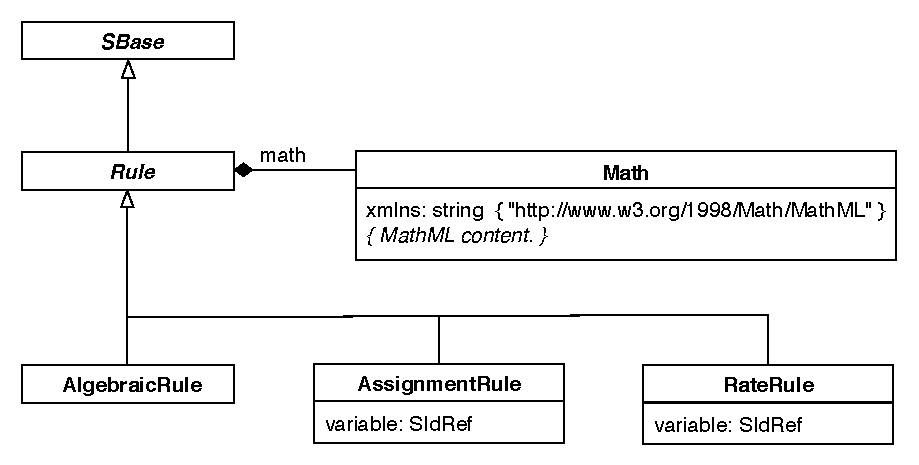
\includegraphics[scale=0.8]{figs/rule-uml}
  \caption{The definition of \RuleUpright and derived types
      \AlgebraicRule, \AssignmentRule and \RateRule.}
  \label{fig:rules}
\end{figure}



\subsubsection{Common attributes in \abstractclass{Rule}}
\label{sec:rule-math}\label{sec:rule-fields}\label{sec:rule-sboterm}

The classes derived from \Rule inherit \token{math} and
  the attributes and elements from \SBase, including
\token{sboTerm}.


\paragraph{The \token{math} element}

A \Rule object has a required element called \token{math},
containing a MathML expression defining the mathematical formula
of the rule.  This MathML formula must return a numerical value.
The formula can be an arbitrary expression referencing the
variables and other entities in an SBML model.  The interpretation
of \token{math} and its associated unit of measurement are
described in more detail in Sections~\ref{sec:algebraicrule},
\ref{sec:assignmentrule} and~\ref{sec:raterule} below.


\paragraph{The \token{sboTerm} attribute}

\Rule inherits an optional \token{sboTerm}
attribute of type \primtype{SBOTerm} from its parent
class \SBase (see Sections~\ref{sec:sboterm-type}
and~\ref{sec:sboTerm}).  When a value is given to this
attribute in an \AlgebraicRule, \AssignmentRule, or
\RateRule instance, it should be an
SBO identifier belonging to the branch for type  \AlgebraicRule, \AssignmentRule, or
\RateRule indicated in Table~\ref{tab:sboterm-availability}.  The relationship is
of the form ``the rule \emph{is-a} X'', where X is
the SBO term.  The term chosen should be the most precise (narrow)
one that captures the role of the rule in the model.

As discussed in Section~\ref{sec:sboTerm}, SBO labels are optional
information on a model.  Applications are free to ignore
\token{sboTerm} values.  A model must be interpretable without the
benefit of SBO labels.


\subsubsection{\class{AlgebraicRule}}
\label{sec:algebraicrule}

The rule type \AlgebraicRule is used to express equations that are
neither assignments of model variables nor rates of change.  The
\AlgebraicRule class does not add any attributes to the basic
\Rule; its role is simply to distinguish this case from the other
cases.  An example of the use of \AlgebraicRule is given in
Section~\ref{sec:algeraiceg}.

In the context of a simulation, algebraic rules are in effect at
all times, $t \geq 0$.  To allow evaluating expressions that
involve the \emph{delay} \token{csymbol}
(Section~\ref{sec:csymbol-token}), algebraic rules are considered
to apply also at $t \leq 0$.  Section~\ref{sec:before-t0}
describes the semantics of assignments, rules, and entity values
for simulation time $t \leq 0$.

An SBML model must not be overdetermined.  The ability to define
arbitrary algebraic expressions in an SBML model introduces the
possibility that a model is mathematically overdetermined by the
overall system of equations constructed from its rules, reactions
and events.  Therefore, if an algebraic rule is introduced in a
model, for at least one of the entities referenced in the rule's
\token{math} element the value of that entity must not be
completely determined by other constructs in the model.  This
means that at least this entity must not have the attribute
\token{constant}=\val{true} and there must also not be a rate rule
or assignment rule for it.  Furthermore, if the entity is a
\Species object, its value must not be determined by reactions,
which means that it must either have the attribute
\token{boundaryCondition}=\val{true} or else not be involved in
any reaction at all.  These restrictions are explained in more
detail in Section~\ref{sec:ruleconstraints} below.

Reaction identifiers can be referenced in the \token{math} 
expression of an algebraic rule, but reaction rates can never be
\emph{determined} by algebraic rules.  This is true even when a
reaction does not contain a \KineticLaw element.  (In such cases
of missing \KineticLaw elements, the model is valid but 
incomplete; the rates of reactions lacking kinetic laws are
simply undefined, and not determined by the algebraic rule.)


\subsubsection{\class{AssignmentRule}}
\label{sec:assignmentrule}

The rule type \AssignmentRule is used to express equations that
set the values of variables.  The left-hand side (the
\token{variable} attribute) of an assignment rule can refer to the
identifier of a \Species, \SpeciesReference, \Compartment, 
or global \Parameter object in
the model (but not a reaction).  The entity identified must not
have its \token{constant} attribute set to \val{true}.  The effects of
an \AssignmentRule are in general terms the same, but differ in
the precise details depending on the type of variable being set:

\begin{itemize}
  
\item \emph{In the case of a species}, an \AssignmentRule sets the
  referenced species' quantity (whether a \quantity{concentration}
  or \quantity{amount}) to the value determined by the formula in
  \token{math}.  The unit associated with the value produced by
  the \token{math} formula should be equal to the unit associated
  with the species' quantity.  (See
  Section~\ref{sec:species-units} for an explanation of how a
  species' quantity is determined.)
  
  \emph{Restrictions}: There must not be both an \AssignmentRule
  \token{variable} attribute and a \SpeciesReference \token{species}
  attribute having the same value, unless that species has its
  \token{boundaryCondition} attribute set to \val{true}.  In other
  words, an assignment rule cannot be defined for a species that
  is created or destroyed in a reaction unless that species is
  defined as a boundary condition in the model.

\item \emph{In the case of a species reference}, an
  \AssignmentRule sets the stoichiometry of the corresponding
  reactant or product to the value determined by the formula in
  \token{math}.  The unit associated with the value produced by
  the \token{math} formula should be consistent with the unit
  \token{dimensionless}, because reactant and product
  stoichiometries in reactions are dimensionless quantities.

\item \emph{In the case of a compartment}, an \AssignmentRule sets
  the referenced compartment's size to the size determined by the
  formula in \token{math}.  The unit associated with the value
  produced by the \token{math} formula should be the same as that
  specified for the compartment's size.  (See
  Section~\ref{sec:compartment-units} for more information about
  compartment units.)
  
\item \emph{In the case of a parameter}, an \AssignmentRule sets
  the referenced parameter's value to the value of the formula in
  \token{math}.  The unit associated with the value produced by
  the formula should be the same as parameter's \token{units}
  attribute value.  (See Section~\ref{sec:parameter-units} for
  more information about parameter units.)

\end{itemize}

In the context of a simulation, assignment rules are in effect at
all times, $t \geq 0$.  For purposes of evaluating expressions
that involve the \emph{delay} \token{csymbol}
(Section~\ref{sec:csymbol-token}), assignment rules are considered
to apply also at $t \leq 0$.  Section~\ref{sec:before-t0} provides
additional information about how $t \leq 0$ should be
  handled.

A model must not contain more than one \AssignmentRule or
\RateRule object having the same value of \token{variable}; in
other words, in the set of all assignment rules and rate rules in
an SBML model, each variable appearing in the left-hand sides can
only appear once.  This simply follows from the fact that an
indeterminate system would result if a model contained more than
one assignment rule for the same variable or both an assignment
rule and a rate rule for the same variable.

Similarly, a model must also not contain \emph{both} an
\AssignmentRule and an \InitialAssignment for the same variable,
because both kinds of constructs apply prior to and at the start
of simulation time, \ie $t \leq 0$.  If a model contained both an
initial assignment and an assignment rule for the same variable,
an indeterminate system would result.  (See also
Section~\ref{sec:initial-assignment-semantics}.)

The value calculated by an \AssignmentRule object overrides the
value assigned to the given symbol by the object defining that
symbol.  For example, if a \Compartment's \token{size} is set in
its definition, and the model also contains an \AssignmentRule
having that compartment's \token{id} as its \token{variable}
value, then the \token{size} assigned in the \Compartment
definition is ignored and the value assigned based on the
computation defined in the \AssignmentRule.  This does \emph{not}
mean that a definition for a given symbol can be omitted if there
is an \AssignmentRule object for it.  For example, there must be a
\Parameter definition for a given parameter if there is an
\AssignmentRule for that parameter.


\subsubsection{\class{RateRule}}
\label{sec:raterule}

The rule type \RateRule is used to express equations that
determine the rates of change of variables.  The left-hand side
(the \token{variable} attribute) can refer to the identifier of a
species, species reference, compartment, or parameter (but not a 
reaction).  The
entity identified must have its \token{constant} attribute set to
\val{false}.  The effects of a \RateRule are in general terms the
same, but differ in the precise details depending on which
variable is being set:

\begin{itemize}
  
\item \emph{In the case of a species}, a \RateRule sets the rate
  of change of the species' quantity (\quantity{concentration} or
  \quantity{amount}) to the value determined by the formula in
  \token{math}.  The unit associated with the rule's \token{math}
  element should be equal to the unit of the species' quantity
  (Section~\ref{sec:species-units}) divided by the model-wide unit
  of \quantity{time} (Section~\ref{sec:timeunits}), or in other
  words, \{unit of \quantity{species quantity}\}/\{unit of
  \quantity{time}\}.

  \emph{Restrictions}: There must not be both a \RateRule
  \token{variable} attribute and a \SpeciesReference \token{species}
  attribute having the same value, unless that species has its
  \token{boundaryCondition} attribute is set to \val{true}.  This
  means a rate rule cannot be defined for a species that is
  created or destroyed in a reaction, unless that species is
  defined as a boundary condition in the model.

\item \emph{In the case of a species reference}, a \RateRule sets
  the rate of change of the stoichiometry of the referenced
  reactant or product to the value determined by the formula in
  \token{math}.  The unit associated with the value produced by
  the formula should be consistent with \{unit derived from
  \token{dimensionless}\}/\{unit of \quantity{time}\}.
  
\item \emph{In the case of a compartment}, a \RateRule sets the
  rate of change of the compartment's size to the value determined
  by the formula in \token{math}.  The unit of the rule's
  \token{math} element should be identical to the compartment's
  \token{units} attribute divided by the model-wide unit of
  \quantity{time}.  (In other words, \{unit of
  \quantity{compartment size}\}/\{unit of \quantity{time}\}.)

\item \emph{In the case of a parameter}, a \RateRule sets the rate
  of change of the parameter's value to that determined by the
  formula in \token{math}.  The unit associated with the rule's
  \token{math} element should be equal to the parameter's
  \token{units} attribute value divided by the model-wide unit of
  \quantity{time}.  (In other words, \{parameter
  \token{units}\}/\{unit of \quantity{time}\}.)

\end{itemize}

In the context of a simulation, rate rules are in effect for
simulation time $t > 0$.  Other types of rules and initial
assignments are in effect at different times;
Section~\ref{sec:before-t0} describes these conditions.

As mentioned in Section~\ref{sec:assignmentrule} for
\AssignmentRule, a model must not contain more than one \RateRule
or \AssignmentRule object having the same value of
\token{variable}; in other words, in the set of all assignment
rules and rate rules in an SBML model, each variable appearing in
the left-hand sides can only appear once.  This simply follows
from the fact that an indeterminate system would result if a model
contained more than one assignment rule for the same variable or
both an assignment rule and a rate rule for the same variable.


\subsubsection{Additional restrictions on rules}
\label{sec:ruleconstraints}

An important design goal of SBML rule semantics is to ensure that
a model's simulation and analysis results will not be dependent on
when or how often rules are evaluated.  To achieve this, SBML
needs to place two additional restrictions on rule use in addition
to the conditions described above regarding the use of
\AlgebraicRule, \AssignmentRule and \RateRule.  The first concerns
algebraic loops in the system of assignments in a model, and the
second concerns overdetermined systems.


\paragraph{The model must not contain algebraic loops}

The combined set of \InitialAssignment, \AssignmentRule and
\KineticLaw objects constitute a set of assignment statements that
should be considered as a whole.  (A \KineticLaw object is counted
as an assignment because it assigns a value to the symbol
contained in the \token{id} attribute of the \Reaction object in which
it is defined.)  This combined set of assignment statements must
not contain algebraic loops---dependency chains between these
statements must terminate.  To put this more formally, consider a
directed graph in which nodes are assignment statements and
directed arcs exist for each occurrence of an SBML species, species reference,
compartment or parameter symbol in an assignment statement's
\token{math} element.  Let the directed arcs point from the
statement assigning the symbol to the statements that contain the
symbol in their \token{math} element expressions.  This graph must
be acyclic.

SBML does not specify when or how often rules should be evaluated.
Eliminating algebraic loops ensures that assignment statements can
be evaluated any number of times without the result of those
evaluations changing.  As an example, consider the following
equations:
\begin{linenomath}
\begin{equation*}
  \begin{array}{lll}
    x = x + 1, & y = z + 200, & z = y + 100
  \end{array}
\end{equation*}
\end{linenomath}
If this set of equations were interpreted as a set of assignment
statements, it would be invalid because the rule for $x$ refers to
$x$ (exhibiting one type of loop), and the rule for $y$ refers to
$z$ while the rule for $z$ refers back to $y$ (exhibiting another
type of loop).

Conversely, the following set of equations would constitute a
valid set of assignment statements:
\begin{linenomath}
\begin{equation*}
  \begin{array}{lll}
    x = 10, & y = z + 200, & z = x + 100
  \end{array}
\end{equation*}
\end{linenomath}


\paragraph{The model must not be overdetermined}

An SBML model must not be overdetermined; that is, a model must
not define more equations than there are unknowns in a model.  An
SBML model without \AlgebraicRule objects cannot be
overdetermined.

Assessing whether a given continuous, deterministic, mathematical
model is overdetermined does not require dynamic analysis; it can
be done by analyzing the system of equations created from the
model.  It should be noted that when a model contains both
reactions and events, there are several sets of equations to
consider in order to assess whether a model is overdetermined.
The set of equations derived from the combined set of rules and
reactions and, for each event, the set of equations derived from
the combined set of rules and event assignments for the particular
event.

One approach is to construct a bipartite graph in which one set of
vertices represents the variables and the other set of vertices
represents the equations.  The approach involves placing edges
between vertices such that variables in the system are linked to
the equations that determine them.  A mathematical model is
overdetermined if the maximal matchings~\citep{chartrand_1977} of
the bipartite graph contain disconnected vertexes representing
equations.  (If one maximal matching has this property, then all
the maximal matchings will have this property; \ie it is only
necessary to find one maximal matching.)
Appendix~\ref{apdx:assessing-overdetermined} describes a method of
applying this procedure to specific SBML data objects.  In some
cases it is possible to avoid the use of an \AlgebraicRule.  This
is discussed in more detail in Section~\ref{sec:bp:rules}.


\subsubsection{Example of rule use}
\label{sec:eg-rule-use}

This section contains an example set of rules.  Consider the
following set of equations:
\begin{linenomath}
  \begin{equation*}
    \begin{array}{lll}
      k = \dfrac{k_3}{k_2}, & s_2 = \dfrac{k \cdot x}{1 + k_2}, & A = 0.10 \cdot x
    \end{array}
  \end{equation*}
\end{linenomath}
This can be encoded by the following scalar rule set (where the
definitions of \texttt{x}, \texttt{s}, \texttt{k}, \texttt{k2},
\texttt{k3} and \texttt{A} are assumed to be located elsewhere in
the model and not shown in this abbreviated example):

\begin{example}
<listOfRules>
    <assignmentRule variable="k">
        <math xmlns="http://www.w3.org/1998/Math/MathML">
            <apply> <divide/> <ci> k3 </ci> <ci> k2 </ci> </apply>
        </math>
    </assignmentRule>
    <assignmentRule variable="s2">
        <math xmlns="http://www.w3.org/1998/Math/MathML">
            <apply>
                <divide/>
                    <apply> <times/> <ci> k </ci> <ci> x </ci> </apply>
                    <apply> <plus/> <cn> 1 </cn> <ci> k2 </ci> </apply>
            </apply>
        </math>
    </assignmentRule>
    <assignmentRule variable="A">
        <math xmlns="http://www.w3.org/1998/Math/MathML">
            <apply> <times/> <cn> 0.10 </cn> <ci> x </ci> </apply>
        </math>
    </assignmentRule>
</listOfRules>
\end{example}


%-----------------------------------------------------------------------------
\subsection{Constraints}
\label{sec:constraints}
%-----------------------------------------------------------------------------

The \Constraint object is a mechanism for stating the
assumptions under which a model is designed to operate.  The
\emph{constraints} are statements about permissible values of
different quantities in a model.  Figure~\ref{fig:constraint}
shows the definition of the \Constraint object class.

\begin{figure}[htb]
  \centering
  \small
  \vspace*{2ex}
  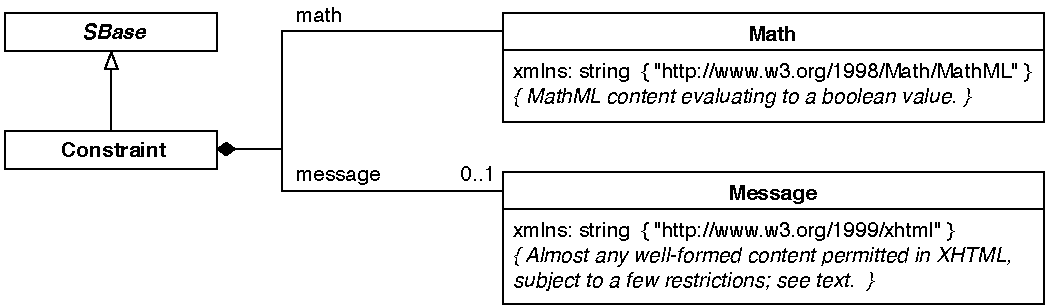
\includegraphics[scale=0.8]{figs/constraint-uml}
  \caption{The definition of class \Constraint.  The contents of
    the \class{Math} class can be any \mathml permitted in SBML,
    but it must return a boolean value.  As shown above, an
    instance of \Constraint can also contain zero or one instances
    of \Message objects; this class of object is simply a wrapper
    (in the XML form, \token{<message> \ldots{} </message>}) for
    XHTML content.  The same guidelines for XHTML content as
    explained in Section~\ref{sec:notes} for notes on \SBaseUpright also
    apply to the XHTML within messages in a \Constraint. A
    sequence of one or more instances of \Constraint objects can
    be located in an instance of \ListOfConstraints in \Model, as
    shown in Figure~\protect\ref{fig:model}.}
  \label{fig:constraint}
\end{figure}

The essential meaning of a constraint is this: if a dynamical
analysis of a model (such as a simulation) reaches a state in
which a constraint is no longer satisfied, the results of the
analysis are deemed invalid beginning with that point in time.
The exact behavior of a software tool, upon encountering a
constraint violation, is left up to the software; \emph{however},
a software tool must somehow indicate to the user when a model's
constraints are no longer satisfied.  (Otherwise, a user may not
realize that the analysis has reached an invalid state and is
potentially producing nonsense results.)  If a software tool does
not have support for constraints, it should indicate this to the
user when encountering a model containing constraints.


\paragraph{The \token{sboTerm} attribute}
\label{sec:constraint-sboterm}

\Constraint inherits an optional \token{sboTerm}
attribute of type \primtype{SBOTerm} from its parent
class \SBase (see Sections~\ref{sec:sboterm-type}
and~\ref{sec:sboTerm}).  When a value is given to this
attribute in a  \Constraint instance, it should be an
SBO identifier belonging to the branch for type  \Constraint
indicated in Table~\ref{tab:sboterm-availability}.  The relationship is
of the form ``the constraint \emph{is-a} X'', where X is
the SBO term.  The term chosen should be the most precise (narrow)
one that captures the role of the constraint in the model.

As discussed in Section~\ref{sec:sboTerm}, SBO labels are optional
information on a model.  Applications are free to ignore
\token{sboTerm} values.  A model must be interpretable without the
benefit of SBO labels.


\subsubsection{The \token{math} element}

\Constraint has one required subelement, \token{math},
containing a MathML formula defining the condition of the
constraint.  This formula must return a boolean value of
\val{true} when the model is in a \emph{valid} state.  The formula
can be an arbitrary expression referencing the variables and other
entities in an SBML model.  The evaluation of \token{math} and
behavior of constraints are described in more detail in
Section~\ref{sec:constraint-semantics} below.


\subsubsection{\class{Message}}
\label{sec:constraint-message}

A \Constraint object can contain an optional element named
\token{message} whose content is determined by object class \Message.
This element can contain a message in XHTML format that may be
displayed to the user when the condition of the constraint in
\token{math} evaluates to a value of \val{false}.  Software tools
are not required to display the message, but it is recommended
that they do so as a matter of best practice.

The XHTML content within a \Message object must follow the same
restrictions as for \Notes objects described in
Section~\ref{sec:notes}.  In particular, the element must declare
the use of the XHTML XML namespace, and must not contain an XML
declaration or a DOCTYPE declaration.


\subsubsection{Semantics of constraints}
\label{sec:constraint-semantics}

In the context of a simulation, a \Constraint has effect at all
times $t \geq 0$.  Each \Constraint's \token{math} element is first
evaluated after any \InitialAssignment definitions in a model at
$t = 0$ and can conceivably trigger at that point.  (In other
words, a simulation could fail a constraint immediately.)

\Constraint definitions \emph{cannot and should not} be used to
compute the dynamical behavior of a model as part of, for example,
simulation.  Constraints may be used as input to non-dynamical
analysis, for instance by expressing flux constraints for flux
balance analysis.

The results of a simulation of a model containing a constraint are
invalid from any simulation time at and after a point when the
function given by the \token{math} returns a value of \val{false}.
Invalid simulation results do not make a prediction of the
behavior of the biochemical reaction network represented by the
model.  The precise behavior of simulation tools is left undefined
with respect to constraints.  If invalid results are detected with
respect to a given constraint, the contents of the \Message
subobject (Section~\ref{sec:constraint-message}) may optionally be
displayed to the user.  The simulation tool may also halt the
simulation or clearly delimit in output data the simulation time
point at which the simulation results become invalid.

There are no restrictions on duplicate \Constraint
definitions or the order of evaluation of \Constraint objects in a
model.  It is possible for a model to define multiple constraints
all with the same \token{math} element.  Since the failure of any
constraint indicates the simulation has entered an invalid state,
a system is not required to attempt detecting whether
other constraints in the model have failed once any one constraint
has failed.


\subsubsection{Example}

As an example, the following SBML fragment demonstrates the
constraint that species \val{S1} should only have values between~1
and~100:

\begin{example}
<model ...>
    ...
    <listOfConstraints>
        <constraint>
            <math xmlns="http://www.w3.org/1998/Math/MathML"
                  xmlns:sbml="http://www.sbml.org/sbml/level3/version1/core">
                <apply>
                    <and/>
                        <apply> 
                          <lt/> 
                          <cn sbml:units="mole"> 1 </cn> 
                          <ci> S1 </ci> 
                        </apply>
                        <apply> 
                          <lt/> 
                          <ci> S1 </ci>  
                          <cn sbml:units="mole"> 100 </cn> 
                        </apply>
                </apply>
            </math>
            <message>
                <p xmlns="http://www.w3.org/1999/xhtml"> Species S1 is out of range. </p>
            </message>
        </constraint>
    </listOfConstraints>
    ...
</model>
\end{example}


%-----------------------------------------------------------------------------
\subsection{Reactions}
\label{sec:reactions}
%-----------------------------------------------------------------------------

A \emph{reaction} in SBML represents any kind of process that can
change the quantity of one or more species in a model.  Examples
of such processes can include transformation, transport, molecular
interactions, and more.  In SBML, the notion of a reaction is
generalized to allow entities that may not be chemical substances;
thus, a reaction in SBML does not necessarily have to be a
biochemical reaction---a biochemical reaction is just one possible
kind of process.

At minimum, to describe a reaction in SBML, it is necessary to
define its \emph{structural} properties, specifically the
participating reactants and/or products (and their corresponding
stoichiometries) and the reversibility of the process.  In
addition, an SBML reaction can also contain a \emph{quantitative}
description of the rate of the reaction; this aspect consists of a
mathematical formula expressing describing the rate at which the
reaction process takes place, together with an optional list of
modifier species and parameters influencing the reaction rate.
The various parts of a reaction are recorded in the SBML \Reaction
object class and other supporting data classes, defined in
Figure~\vref{fig:reaction}.

\begin{figure}[b]
  \centering
  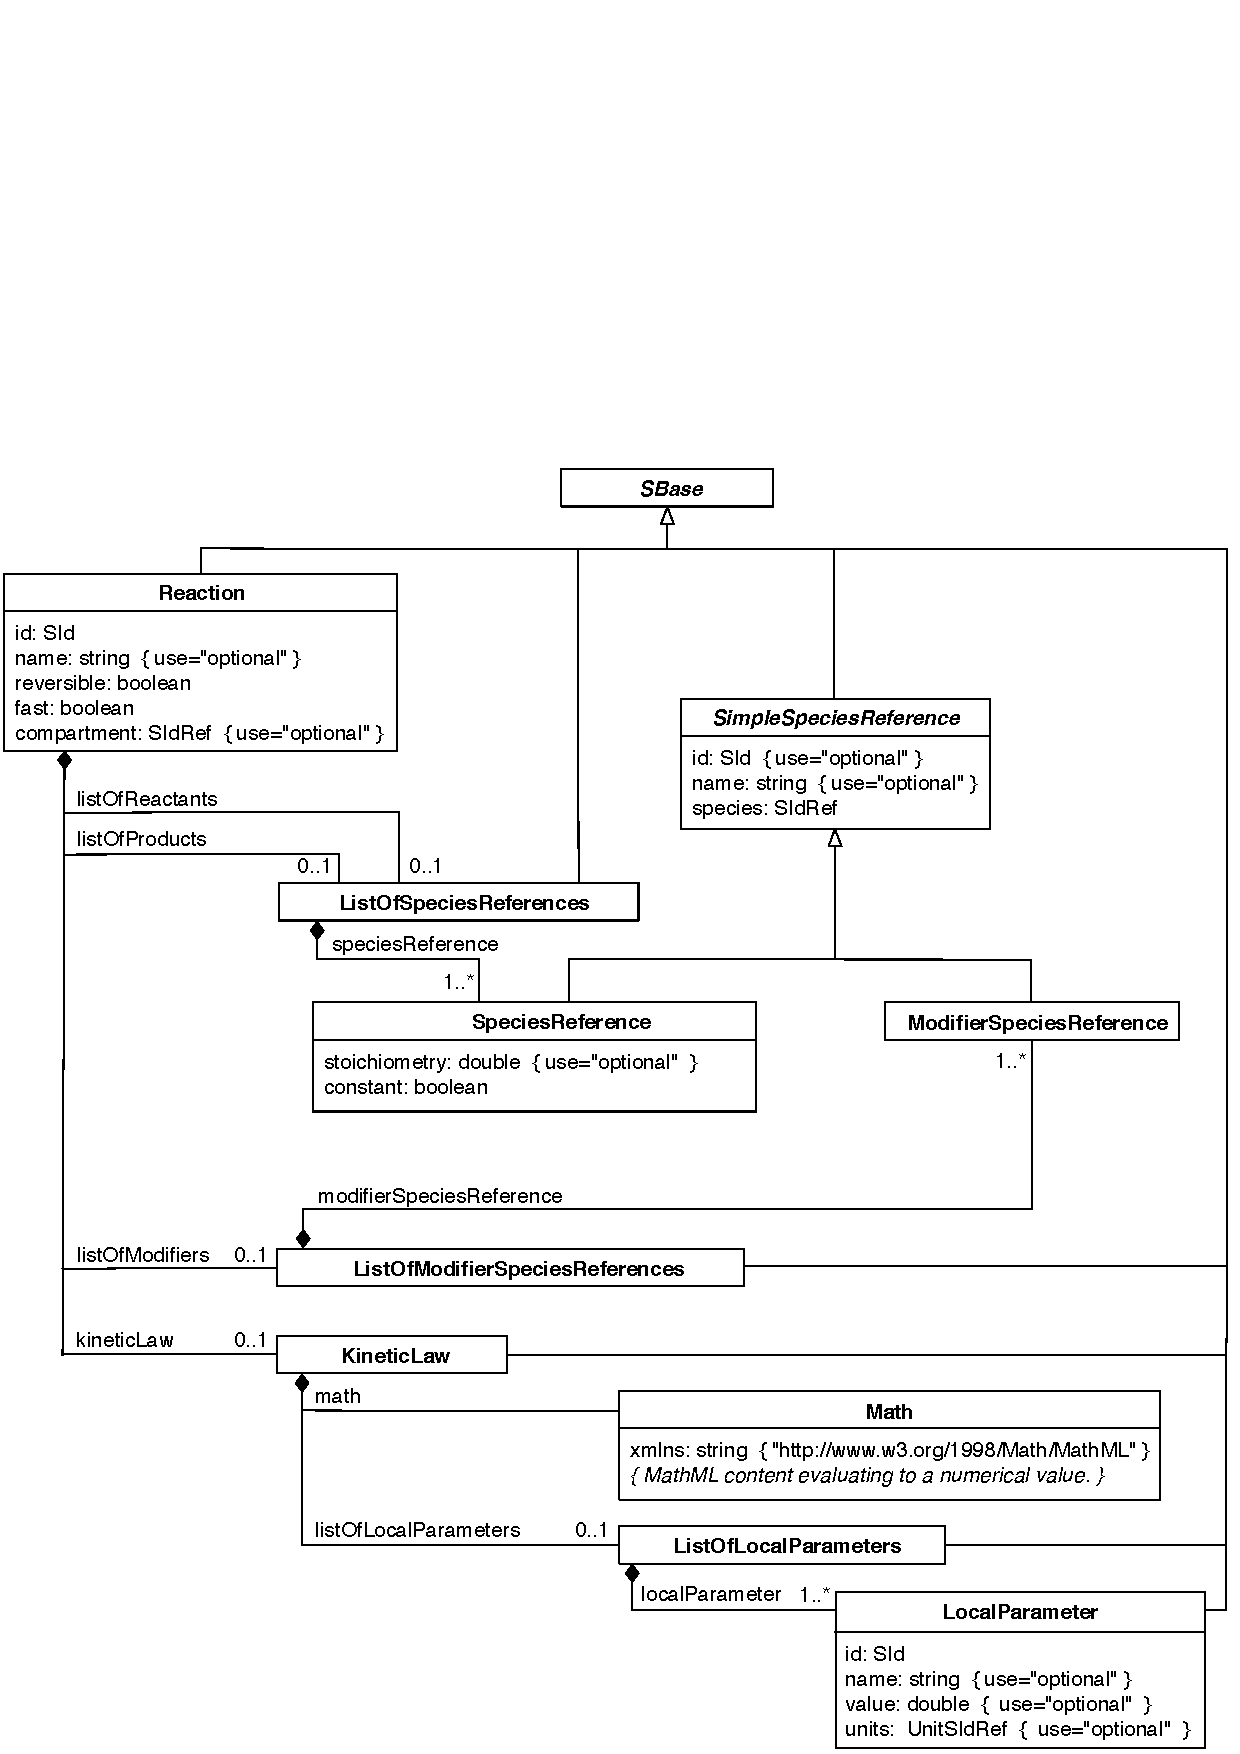
\includegraphics[scale=0.78]{figs/reaction-uml-v2}
  \caption{The definitions of \Reaction, \KineticLaw,
    \SpeciesReference, \ModifierSpeciesReference, \LocalParameter,
    as well as the container classes \ListOfSpeciesReferences,
    \ListOfModifierSpeciesReferences, and \ListOfLocalParameters.
    Note that \SimpleSpeciesReferenceUpright is an abstract class used
    only to provide some common attributes to its derived
    classes.}
  \label{fig:reaction}
\end{figure}


\subsubsection{\class{Reaction}}
\label{sec:reaction-type}
\label{sec:listofreactants}
\label{sec:listofproducts}
\label{sec:listofmodifiers}

Each reaction in an SBML model is defined using an instance of a
\Reaction object.  As shown in Figure~\vref{fig:reaction}, it
contains several scalar attributes and several lists of other
objects.


\paragraph{The \token{id} and \token{name} attributes}

As with most other main kinds of objects in SBML, the
\Reaction object class
includes a mandatory attribute called \token{id}, of type
\primtype{SId}, and an optional attribute \token{name}, of type
\primtype{string}.  The \token{id} attribute is used to give the
reaction a unique identifier in the model.  This identifier can be
used in mathematical formulas elsewhere in an SBML model to
represent the rate of that reaction; this usage is explained in
detail in Section~\ref{subsec:reaction-as-symbol} below.  The
\token{name} attribute can be used to give the reaction a more
free-form, descriptive name.  The \token{name} and \token{id}
attributes must be used as described in
Section~\ref{sec:idnameattribs}.


\paragraph{The lists of reactants, products and modifiers}

Each species participating as a reactant, product, and/or modifier
in a reaction must be declared using a \SpeciesReference and/or
\ModifierSpeciesReference object stored in the list elements
\token{listOfReactants}, \token{listOfProducts} and
\token{listOfModifiers}.  The object classes \SpeciesReference and
\ModifierSpeciesReference are described in more detail in
Sections~\ref{subsec:speciesreference}
and~\ref{subsec:modifierreference} below.  Throughout this text,
we use the informal expressions ``list of reactants'', ``list of
products'' and ``list of modifiers'' to mean, respectively, the
list of species identified by \SpeciesReference objects within a
\Reaction \token{listOfReactants} element, the list of species
identified by \SpeciesReference objects within a \Reaction
\token{listOfProducts} element, and the list of species identified
by \ModifierSpeciesReference objects within a \Reaction
\token{listOfModifiers} element.

Certain restrictions are placed on the appearance of species in
reaction definitions:
\begin{itemize}
  
\item The ability of a species to appear as a reactant or product
  of any reaction in a model is governed by certain combinations
  of the attributes \token{constant} and \token{boundaryCondition}
  on the \Species object instance; see
  Section~\ref{sec:species-constant} for more information.
  
\item Any species appearing in the \token{math} element of the
  \token{kineticLaw} of a \Reaction instance must be declared in
  at least one of that \Reaction's lists of reactants, products,
  and/or modifiers.  It is an error for a reaction's kinetic law
  formula to refer to species that have not been declared for that
  reaction.
  
\item A reaction definition can contain an empty list of reactants
  \emph{or} an empty list of products, but it must have at least
  one reactant or product; in other words, a reaction without any
  reactant or product species is not permitted.  (This restriction
  does not apply to modifier species, which are always optional.)

\end{itemize}


\paragraph{The \token{kineticLaw} element}

A \Reaction object can contain up to one \KineticLaw object, in
the \token{kineticLaw} element.  This ``kinetic law'' defines the
speed at which the process defined by the reaction takes place.  A
more detailed description of \KineticLaw is left to
Section~\ref{subsec:kinetic-law} below.

The inclusion of a \KineticLaw object in an instance of a
\Reaction is optional.  For some modeling purposes, models
containing reactions without defined rates are an acceptable
alternative (and may even be the only possible option, such as
when the kinetics of the reactions are unknown).  However, missing
kinetic laws preclude the application of many model analysis
techniques, including simulation.


\paragraph{The \token{reversible} attribute}
\label{sec:reversible}

The mandatory boolean attribute \token{reversible} on \Reaction
indicates whether the reaction is reversible.  To say that a
reaction is \emph{reversible} is to say it can proceed in either
the forward or the reverse direction.  This information may be
redundant in cases where the reversibility of the reaction can be
deduced by inspecting the rate formula given in the kinetic law.
However, a reaction is not required to have a kinetic law, and
besides, when a rate expression is present, it may not always be
possible to deduce the reversibility by inspecting it.  Having a
separate attribute for \token{reversible} allows certain kinds of
structural analysis, such as elementary mode analysis, even in
these cases.

Mathematically, the \token{reversible} attribute on \Reaction has
no impact on the construction of the equations for change of the
species quantities.  However, labeling a reaction as irreversible
is interpreted as an assertion that the rate expression will not
have negative values during a simulation.  Software developers may
wish to provide their software systems with a means of testing
that this condition holds.

The presence of reversibility information in two places (\ie the
rate expression in the kinetic law, and the \token{reversible}
flag) leaves open the possibility that a model could contain
contradictory information, but this would be considered to be an
error of the encoded model, rather than an invalid SBML encoding.


\paragraph{The \token{fast} attribute}
\label{sec:fast}

The boolean attribute \token{fast} is another required boolean
attribute of \Reaction.  When a model contains a value of
\val{true} for \token{fast} on any of its reactions, it indicates
that the creator of the model is distinguishing different time
scales of reactions in the system.  If a model does not
distinguish between time scales, the \token{fast} attribute should
be set to \val{false} for all reactions.

The model's reactions are divided into two sets by the
values of the \token{fast} attributes.  The set of reactions
having \token{fast}=\val{true} (known as \emph{fast reactions})
should be assumed to be operating on a time scale significantly
faster than the other reactions (the \emph{slow reactions}).  Fast
reactions are considered to be instantaneous relative to the slow
reactions.  Software tools should use a pseudo steady-state
approximation for the set of fast reactions when constructing the
system of equations for the model.  More specifically, the set of
reactions that have the \token{fast} attribute set to \val{true}
forms a subsystem that should be described by a pseudo
steady-state approximation in relationship to all other reactions
in the model.  Under this description, relaxation from any initial
condition or perturbation from any intermediate state of this
subsystem would be infinitely fast.
Appendix~\ref{apdx:consequences-of-being-fast} provides a
technical explanation of an approach to solving systems with fast
reactions.

The correctness of the approximation requires a significant
separation of time scales between the fast reactions and other
processes.  It is the responsibility of the modeler or of the
software system writing the SBML model to ensure this condition is
fulfilled.

Note that the \token{fast} attribute has a significant effect on
the mathematical interpretation of a model and cannot be safely
ignored if a software tool does not implement support for the
corresponding concept.  Software systems should indicate to users
when they encounter models with reactions having
\token{fast}=\val{true} and do not have the capacity to analyze
the model using a pseudo steady-state approximation.


\paragraph{The \token{compartment} attribute on \class{Reaction}}
\label{sec:reaction-compartment}

The optional attribute \token{compartment}, of data type
\primtype{SIdRef}, can be used to indicate the compartment in
which the reaction is assumed to take place.  If the attribute is
present, its value must be the identifier of a \Compartment object
defined in the enclosing \Model object.

Similar to the \token{reversible} attribute, the value of the
\token{compartment} attribute has no direct impact on the
construction of mathematical equations for the SBML model.  When a
reaction has a kinetic law, the compartment location may already
be implicit in the kinetic law (though this cannot always be
guaranteed).  Nevertheless, software tools may find the
\token{compartment} attribute value useful for such purposes as
analyzing the structure of the model, guiding the modeler in
constructing correct rate formulas, and visualization.


\paragraph{The \token{sboTerm} attribute on \class{Reaction}}
\label{sec:reaction-sboterm}

\Reaction inherits an optional \token{sboTerm}
attribute of type \primtype{SBOTerm} from its parent
class \SBase (see Sections~\ref{sec:sboterm-type}
and~\ref{sec:sboTerm}).  When a value is given to this
attribute in a  \Reaction instance, it should be an
SBO identifier belonging to the branch for type  \Reaction  
indicated in Table~\ref{tab:sboterm-availability}.  The relationship is
of the form ``the reaction \emph{is-a} X'', where X is
the SBO term.  The term chosen should be the most precise (narrow)
one that captures the role of the reaction in the model.

As discussed in Section~\ref{sec:sboTerm}, SBO labels are optional
information on a model.  Applications are free to ignore
\token{sboTerm} values.  A model must be interpretable without the
benefit of SBO labels.


\subsubsection{\class{SimpleSpeciesReference}}
\label{subsec:simplespeciesreference}

As mentioned above, every species that enters into a given
reaction must appear in that reaction's lists of reactants,
products and/or modifiers.  In an SBML model, all species that may
participate in any reaction are listed in the \ListOfSpecies
object of the top-level \Model object instance (see
Section~\ref{sec:model}).  The lists of products, reactants and
modifiers in \Reaction objects do not introduce new species, but
rather, they refer back to those listed in the model's top-level
\ListOfSpecies object.  For reactants and products, the connection
is made using a \SpeciesReference object; for modifiers, it is
made using a \ModifierSpeciesReference object.
\SimpleSpeciesReference, defined in Figure~\vref{fig:reaction}, is
an abstract type that serves as the parent class of both
\SpeciesReference and \ModifierSpeciesReference.  It is used
simply to hold the attributes and elements that are common to the
latter two objects.


\paragraph{The \token{id} and \token{name} attributes}

\SimpleSpeciesReference has optional attributes for an identifier
(\token{id}, of data type \primtype{SId}) and name (\token{name},
of data type \primtype{string}).  The \token{id} and \token{name}
attributes must be used as described in
Section~\ref{sec:idnameattribs}.

The \token{id} value (whether it is in a \SpeciesReference or
\ModifierSpeciesReference object) exists in the global namespace
of the model.  In SBML \thisLV, the only meaning defined for the
use of such identifiers concerns the \token{id} of a
\SpeciesReference object (discussed further in
Section~\ref{subsec:speciesreference}); no meaning or value is
associated with the identifiers of \ModifierSpeciesReference.
However, the identifiers are present on both object classes for
possible use by SBML Level~3 packages.


\paragraph{The \token{species} attribute}

The \SimpleSpeciesReference object class has a required attribute,
\token{species}, of data type \primtype{SIdRef}.  As with the
other attributes, it is inherited by \SpeciesReference and
\ModifierSpeciesReference.  The value of \token{species} must be
the identifier of a species defined in the enclosing \Model; the
referenced species is thereby declared as participating in the
reaction being defined.  The precise role of that species as a
reactant, product, or modifier in the reaction is determined by
the subtype of \SimpleSpeciesReference (\ie either
\SpeciesReference or \ModifierSpeciesReference) in which the
identifier appears and by the specific list of species references
in which the \SpeciesReference appears.


\paragraph{The \token{sboTerm} attribute}
\label{sec:simplespeciesreference-sboterm}

\SimpleSpeciesReference inherits an optional \token{sboTerm}
attribute of type \primtype{SBOTerm} from its parent class \SBase
(see Sections~\ref{sec:sboterm-type} and~\ref{sec:sboTerm}).  When
a value is given to this attribute in a \SimpleSpeciesReference
instance, it should be an SBO identifier belonging to the branch
for type \SimpleSpeciesReference indicated in
Table~\ref{tab:sboterm-availability}.  The relationship is of the
form ``the species reference \emph{is-a} X'', where X is the SBO
term.  The term chosen should be the most precise (narrow) one
that captures the role of the species reference in the model.

As discussed in Section~\ref{sec:sboTerm}, SBO labels are optional
information on a model.  Applications are free to ignore
\token{sboTerm} values.  A model must be interpretable without the
benefit of SBO labels.


\subsubsection{\class{SpeciesReference}}
\label{subsec:speciesreference}

\Reaction provides a way to express which species act as reactants
and which species act as products in a reaction, and to declare
their stoichiometries.  This is done using \SpeciesReference
objects.  As mentioned above in
Section~\ref{subsec:simplespeciesreference}, \SpeciesReference
inherits the mandatory attribute \token{species} and optional
attributes \token{id}, \token{name}, and \token{sboTerm} from the
parent type \SimpleSpeciesReference.  It also defines the optional
attribute \token{stoichiometry} and the mandatory attribute
\token{constant}, described below.


\paragraph{The \token{stoichiometry} attribute}

The {\em stoichiometry} of a species in a reaction describes how
much of the species changes when a reaction event takes place.  In
SBML, product and reactant stoichiometries are specified using the
optional \token{stoichiometry} on \SpeciesReference object.  \changed{The
\token{stoichiometry} attribute is of type \primtype{double}.}  A missing
\token{stoichiometry} implies that the stoichiometry is either
unknown, or to be obtained from an external source, or determined
by an initial assignment (Section~\ref{sec:initialAssignment}) or
other SBML construct elsewhere in the model.

A species reference's stoichiometry is set by its
\token{stoichiometry} attribute exactly once.  If the
\SpeciesReference object's \token{constant} attribute (see below)
has the value \val{true}, then the stoichiometry is fixed and
cannot be changed except by an \InitialAssignment.  These two
methods of setting the stoichiometry (\ie using
\token{stoichiometry} directly, or using an \InitialAssignment)
differ in that the \token{stoichiometry} attribute can only be set
to a literal floating-point number, whereas \InitialAssignment
allows the value to be set using an arbitrary mathematical
expression.  (As an example, the approach could be used to set the
stoichiometry to a rational number of the form \emph{p}/\emph{q},
where \emph{p} and \emph{q} are integers, something that is
occasionally useful in the context of biochemical reaction
networks.)  If the species reference's \token{constant} attribute
has the value \val{false}, the species reference's value may be
overridden by an \InitialAssignment or changed by \AssignmentRule
or \AlgebraicRule, and in addition, for simulation time $t > 0$,
it may also be changed by a \RateRule or \Event{}s.  (However,
some of these constructs are mutually exclusive; see
Sections~\ref{sec:rules} and~\ref{sec:events}.)  It is not an
error to define \token{stoichiometry} on a species reference and
also redefine the stoichiometry using an \InitialAssignment, but
the \token{stoichiometry} attribute in that case is ignored.
Section~\ref{sec:before-t0} provides additional information about
the semantics of assignments, rules and values for simulation time
$t \leq 0$.

An explanation of how exactly the stoichiometry is used in the
mathematical interpretation of the model is given in
Section~\ref{sec:about-kinetic-laws}.


\paragraph{The \token{constant} attribute}

The \SpeciesReference attribute \token{constant} is a
mandatory boolean attribute used to indicate whether the
\token{stoichiometry} value can vary during a simulation.  If
\token{constant}=\val{true}, the corresponding species'
stoichiometry in the reaction cannot be changed by other
constructs elsewhere in the model except by an \InitialAssignment.
A value of \val{false} means the stoichiometry can be changed by
other SBML constructs such as rules (see Section~\ref{sec:rules}),
as described above in the section on the \token{stoichiometry}
attribute.


\paragraph{Use of species reference identifiers in mathematical expressions}
\label{sec:reaction:speciesReferences-in-mathematical-expressions}

The value of the \token{id} attribute of a \SpeciesReference can
be used as the content of a \token{ci} element in MathML formulas
elsewhere in the model.  When the identifier appears in a \token{ci}
element, it represents the stoichiometry of the corresponding
species in the reaction where the \SpeciesReference object
instance appears.  More specifically, it represents the value of
the \token{stoichiometry} attribute on the \SpeciesReference
object.


\paragraph{The unit of measurement associated with a
  \class{SpeciesReference}'s stoichiometry value}
\label{sec:speciesreferences-units}

The unit associated with the value of a species' stoichiometry is
always considered to be \token{dimensionless}.  This has the
following implications:
\begin{itemize}

\item When a species reference's identifier appears in
  mathematical formulas elsewhere in the model, the unit
  associated with that value is \token{dimensionless}.

\item The units of the \token{math} elements of \AssignmentRule,
  \InitialAssignment and \EventAssignment objects setting the
  stoichiometry of the species reference should be
  \token{dimensionless}.

\item If a species reference's identifier is the subject of a
  \RateRule, the unit associated with the \RateRule object's value
  should be \token{dimensionless}/\quantity{time}, where
  \quantity{time} is the model-wide unit of \token{time}
  (Section~\ref{sec:timeunits}).

\end{itemize}


\paragraph{Examples}

The following is a simple example of a species reference for
species \val{X0}, with stoichiometry \val{2}, in a list of
reactants within a reaction having the identifier \val{J1}:

\begin{example}
<model ...>
    ...
    <listOfReactions>
        <reaction id="J1" reversible="false" fast="false">
            <listOfReactants>
                <speciesReference species="X0" stoichiometry="2" constant="true"/>
            </listOfReactants>
            ...
        </reaction>
        ...
    </listOfReactions>
    ...
</model>
\end{example}

The following is a more complex example of a species reference
with an id \val{sr01} and an initial assignment that assigns a
rational number to the stoichiometry:

\begin{example}
<model ...>
    ...
    <listOfInitialAssignments>
        <initialAssignment symbol="sr01">
            <math xmlns="http://www.w3.org/1998/Math/MathML"
                  xmlns:sbml="http://www.sbml.org/sbml/level3/version1/core">
                <cn type="rational" sbml:units="dimensionless"> 3 <sep/> 2 </cn>
            </math>
        </initialAssignment>
        ...
    </listOfInitialAssignments>
        ...
    <listOfReactions>
        <reaction id="J1" reversible="true" fast="false">
            <listOfReactants>
                <speciesReference id="sr01" species="X0" constant="true"/>
            </listOfReactants>
            ...
        </reaction>
        ...
    </listOfReactions>
    ...
</model>
\end{example}


A species can occur more than once in the lists of reactants and
products of a given \Reaction instance.  The effective
stoichiometry for the species is the sum of the stoichiometry
values given in the \SpeciesReference objects in the list of
products \emph{minus} the sum of stoichiometry values given in the
\SpeciesReference objects in the list of reactants.  A positive
value indicates the species is effectively a product and a
negative value indicates the species is effectively a reactant.
SBML places no restrictions on the effective stoichiometry of a
species in a reaction; for example, it can be zero.  In the
following SBML fragment, the two reactions have the same effective
stoichiometry for all their species:

\begin{example}
<reaction id="x" reversible="false" fast="false">
    <listOfReactants>
        <speciesReference species="a" stoichiometry="1" constant="true"/>
        <speciesReference species="a" stoichiometry="1" constant="true"/>
        <speciesReference species="b" stoichiometry="1" constant="true"/>
    </listOfReactants>
    <listOfProducts>
        <speciesReference species="c" stoichiometry="1" constant="true"/>
        <speciesReference species="b" stoichiometry="1" constant="true"/>
    </listProducts>
</reaction>
<reaction id="y" reversible="false" fast="false">
    <listOfReactants>
        <speciesReference species="a" stoichiometry="2" constant="true"/>
    </listOfReactants>
    <listOfProducts>
        <speciesReference species="c" stoichiometry="1" constant="true"/>
    </listProducts>
</reaction>
\end{example}



\subsubsection{\class{ModifierSpeciesReference}}
\label{subsec:modifierreference}

Sometimes a species appears in the kinetic rate formula of a
reaction but is neither created nor destroyed in that reaction
(for example, because it acts as a catalyst or inhibitor).  In
SBML, all such species are simply called \emph{modifiers} without
regard to the detailed role of those species in the model (though
a model could use SBO terms to clarify the roles; see
Section~\ref{sec:sbo}).  The \Reaction object class provides a way
to express which species act as modifiers in a given reaction.
This is the purpose of the list of modifiers available in
\Reaction.  The list contains instances of
\ModifierSpeciesReference object.

As shown in Figure~\vref{fig:reaction}, the
\ModifierSpeciesReference class inherits the mandatory attribute
\token{species} and optional attributes \token{id} and
\token{name} from the parent class \SimpleSpeciesReference; see
Section~\ref{subsec:simplespeciesreference} for their precise
definitions.  As already explained in
Section~\ref{subsec:simplespeciesreference}, no meaning is
assigned to the identifier of \ModifierSpeciesReference object
instances in SBML \thisLV, but the identifiers are available for
possible use by SBML Level~3 packages.  Note also that modifiers
in reactions also have no stoichiometries and therefore do not
possess a \token{stoichiometry} attribute.

The value of the \token{species} attribute must be the identifier of a
species defined in the enclosing \Model; this species is
designated as a modifier for the current reaction.  A reaction may
have any number of modifiers.  It is permissible for a modifier
species to appear simultaneously in the list of reactants and
products of the same reaction where it is designated as a
modifier, as well as to appear in the list of reactants, products
and modifiers of other reactions in the model.


\subsubsection{\class{KineticLaw}}
\label{subsec:kinetic-law}
\label{subsec:listoflocalparameters}

The \KineticLaw object class is used to describe the rate at which
the process defined by the \Reaction takes place.  As shown in
Figure~\vref{fig:reaction}, \KineticLaw has elements called
\token{math} and \token{listOfLocalParameters}, in addition to the
attributes and elements it inherits from \SBase.


\paragraph{The \token{math} element}

As shown in Figure~\vref{fig:reaction}, \KineticLaw has an element
called \token{math} for holding a MathML formula defining the rate
of the reaction.  The expression in \token{math} may refer to
global identifiers defined in the model as well as \LocalParameter object
identifiers from the \KineticLaw's list of local parameters (see
below).  However, the only \Species identifiers that can be used
in \token{math} are those declared in the lists of reactants,
products and modifiers in the \Reaction object (see
Sections~\ref{subsec:simplespeciesreference},
\ref{subsec:speciesreference} and~\ref{subsec:modifierreference}).

Section~\ref{sec:about-kinetic-laws} provides important
discussions about the meaning and interpretation of SBML ``kinetic
laws''.


\paragraph{The list of local parameters}

An instance of \KineticLaw can contain a list of one or more
\LocalParameter objects (Section~\ref{subsec:localparameter})
defining new parameters whose identifiers can be used in the
\token{math} formula.  These ``local parameters'' are optional---a
kinetic law can always refer to global \Parameter objects.  The
local parameter facility simply provides a way to add additional
parameters that may be relevant only to a specific reaction, and
that may therefore be better handled by encapsulating their
definitions within that kinetic law.

As discussed in Section~\ref{sec:identifiers}, reactions introduce
local namespaces for local parameter identifiers, and within a
\KineticLaw object, a local parameter whose identifier is
identical to a global identifier defined in the model takes
precedence over the value associated with the global identifier.
Note that this introduces the potential for a local parameter
definition to shadow a global identifier.  SBML does not separate
symbols by class of object; consequently, inside the kinetic law
mathematical formula, the value of a local parameter having the
same identifier as a species, compartment, parameter or other
global model entity will override the global value.  Modelers and
software developers may wish to take precautions to avoid this
happening accidentally.


\paragraph{The \token{sboTerm} attribute}

\KineticLaw  inherits an optional \token{sboTerm}
attribute of type \primtype{SBOTerm} from its parent
class \SBase (see Sections~\ref{sec:sboterm-type}
and~\ref{sec:sboTerm}).  When a value is given to this
attribute in a  \KineticLaw instance, it should be an
SBO identifier belonging to the branch for type  \KineticLaw
indicated in Table~\ref{tab:sboterm-availability}.  The relationship is
of the form ``the kinetic law \emph{is-a} X'', where X is
the SBO term.  The term chosen should be the most precise (narrow)
one that captures the role of the kinetic law in the model.

As discussed in Section~\ref{sec:sboTerm}, SBO labels are optional
information on a model.  Applications are free to ignore
\token{sboTerm} values.  A model must be interpretable without the
benefit of SBO labels.


\subsubsection{\class{LocalParameter}}
\label{subsec:localparameter}

The \KineticLaw object within a \Reaction object can contain a
\ListOfLocalParameters object containing the definitions of
\emph{local parameter} that are only accessible by the kinetic law
formula of that particular reaction.  The list contains
\LocalParameter objects, each of which associates an identifier
with a value.  This identifier can then be used in the kinetic
law.  The definition of \LocalParameter is shown in
Figure~\vref{fig:reaction}.


\paragraph{The \token{id} and \token{name} attributes}

\LocalParameter has a required attribute \token{id}, of data type
\primtype{SId}, to give the local parameter an identifier by which
the kinetic law formula can refer to it.  A local parameter can
also have an optional \token{name} attribute of type
\primtype{string}.  The identifier of a local parameter needs to
be unique only within the list of local parameters of one
reaction.  The details about the scope for identifiers are given
in Sections~\ref{sec:identifiers}
and~\ref{subsec:listoflocalparameters}, and about the use of names
in Section~\ref{sec:name}.


\paragraph{The \token{value} attribute}

The optional attribute \token{value} determines the value (of type
\primtype{double}) assigned to the identifier.  A missing
\token{value} attribute implies that the value either is unknown,
or to be obtained from an external source.  (Note that, unlike the
case with global \Parameter objects, there is no way in SBML
\thisLV for \InitialAssignment or other SBML constructs to be used
for setting the value of \LocalParameter objects, because local
parameters are local to reactions.)


\paragraph{The \token{units} attribute}

The unit of measurement associated with the value of the parameter
can be specified using the optional attribute \token{units}.  The
attribute's value must have the data type \primtype{UnitSIdRef}
(Section~\ref{sec:unitsidref}).  There are no constraints on the
units that can be assigned to local parameters in a model; there
are also no units to inherit from the enclosing \Model object
(unlike the case for, e.g., \Species and \Compartment).

The \token{units} attribute is used in the following way: when a
local parameter's identifier appears in the content of the
\token{math} element of the enclosing \KineticLaw object, the unit
of measurement associated with the local parameter's value is
determined by the \LocalParameter object's \token{units}
attribute.


\paragraph{The \token{sboTerm} attribute}

\LocalParameter inherits an optional \token{sboTerm} attribute of
type \primtype{SBOTerm} from its parent class \SBase (see
Sections~\ref{sec:sboterm-type} and~\ref{sec:sboTerm}).  When a
value is given to this attribute in a \LocalParameter instance, it
should be an SBO identifier belonging to the branch for type
\LocalParameter indicated in Table~\ref{tab:sboterm-availability}.
The relationship is of the form ``the local parameter \emph{is-a}
X'', where X is the SBO term.  The term chosen should be the most
precise (narrow) one that captures the role of the local parameter
in the model.

As discussed in Section~\ref{sec:sboTerm}, SBO labels are optional
information on a model.  Applications are free to ignore
\token{sboTerm} values.  A model must be interpretable without the
benefit of SBO labels.


\paragraph{Example}

The following is an example of a \Reaction object that defines a
reaction with identifier $J_1$, in which $X_0 \rightarrow S_1$ at
a rate given by $k \cdot [X_0] \cdot [S_2]$, where $S_2$ is a
catalyst and $k$ is a parameter, and the square brackets
symbolizes that the species quantities are in terms of
concentrations.  The reaction is assumed to take place all in one
compartment identified as \val{c1}.  The example demonstrates the
use of species references, \KineticLaw objects and local
parameters.  The units associated with the species identifiers
here are \quantity{amount}/\quantity{volume} (see
Section~\ref{sec:species}), and so the rate expression $k \cdot
[X_0] \cdot [S_2]$ needs to be multiplied by the compartment
volume (represented by its identifier, \val{c1}) to produce the
desired units of \quantity{amount}/\quantity{time} for the rate
expression.

\begin{example}
<model timeUnits="second" extentUnits="mole" substanceUnits="mole">
    <listOfUnitDefinitions>
        <unitDefinition id="per_concent_per_time">
            <listOfUnits>
                <unit kind="litre"  exponent="1"  scale="0" multiplier="1"/>
                <unit kind="mole"   exponent="-1" scale="0" multiplier="1"/>
                <unit kind="second" exponent="-1" scale="0" multiplier="1"/>
            </listOfUnits>
        </unitDefinition>
    </listOfUnitDefinitions>
    <listOfCompartments>
        <compartment id="c1" units="litre" size="0.001" spatialDimensions="3" constant="true"/>
    </listOfCompartments>
    <listOfSpecies>
        <species id="S1" compartment="c1" initialConcentration="2.0" 
                 hasOnlySubstanceUnits="false" boundaryCondition="false" constant="false"/>
        <species id="S2" compartment="c1" initialConcentration="0.5" 
                 hasOnlySubstanceUnits="false" boundaryCondition="false" constant="false"/>
        <species id="X0" compartment="c1" initialConcentration="1.0" 
                 hasOnlySubstanceUnits="false" boundaryCondition="false" constant="false"/>
    </listOfSpecies>
    <listOfReactions>
        <reaction id="J1" reversible="false" fast="false">
            <listOfReactants>
                <speciesReference species="X0" stoichiometry="1" constant="true"/>
            </listOfReactants>
            <listOfProducts>
                <speciesReference species="S1" stoichiometry="1" constant="true"/>
            </listOfProducts>
            <listOfModifiers>
                <modifierSpeciesReference species="S2"/>
            </listOfModifiers>
            <kineticLaw>
                <math xmlns="http://www.w3.org/1998/Math/MathML">
                    <apply>
                        <times/> <ci> k </ci> <ci> S2 </ci> <ci> X0 </ci> <ci> c1 </ci>
                    </apply>
                </math>
                <listOfLocalParameters>
                    <localParameter id="k" value="0.1" units="per_concent_per_time"/>
                </listOfLocalParameters>
            </kineticLaw>
        </reaction>
    </listOfReactions>
</model>
\end{example}


\subsubsection{Mathematical interpretation of SBML reactions and kinetic laws}
\label{sec:about-kinetic-laws}

In SBML, \emph{reactions} are the central mechanism for describing
processes that change the quantities of species in a model.  The
\emph{kinetic law} of an SBML reaction provides a quantitative
description of the speed with which this happens.  In this
section, we provide an interpretation of SBML kinetic laws in the
framework of a system of ordinary differential equations (ODEs).
However, the choice of ODEs as the framework is only for
exposition purposes here, in order to allow us to present a
concrete mathematical expression of the model in terms that many
readers will be familiar with; it is equally possible to translate
a model into other frameworks, and some formulations, such as
discrete stochastic systems, are indeed quite common.


\paragraph{Semantics of rate law and stoichiometry}

The \emph{stoichiometry} of a species $S$ in a reaction describes
the proportion, relative to other species participating in that
reaction, of $S$ involved in each reaction event.  For example, in
a reaction $S_1 + 2 S_2 \rightarrow S_3$, twice as many entities
of $S_2$ as entities of $S_1$ are involved each time a reaction
event is counted.  The value of the expression in the
\KineticLaw's \token{math} element describes the \emph{rate} at
which the reaction takes place.  The product of the reaction rate
(of a given reaction) and the stoichiometry (of a given species in
the reaction) describes the reaction's contribution to the rate of
change of the species' quantity in the overall system.

It is important to make clear that a ``kinetic law'' in SBML is
\emph{not} identical to a traditional rate law.  When modeling
species as continuous amounts (\eg concentrations), the rate laws
used are traditionally expressed in terms of
\quantity{concentration per time}.  Unfortunately, this approach
only works well in cases where certain assumptions hold.  Three
assumptions in particular are incompatible with generalized
multicompartmental modeling; they are listed in
Table~\ref{tab:rate-law-problems} along with the problems they
entail.

\begin{table}[tbh]
  \centering
  \begin{edtable}{tabular}{p{2.8in}p{3.26in}}
    \toprule
    \textbf{Assumption} & \textbf{Problem}\\
    \midrule
    All species that participate in a given reaction are located
    in one compartment
    &
    SBML must support reaction processes (\eg transport) that
    move species between compartments
    \\[10pt]
    Compartments are three-dimensional volume containers
    &
    SBML must support models where reactions may take place at
    interfaces (\eg 2-D membranes) between compartments, thus
    involving compartments with different dimensions
    \\[10pt]    
    Compartment volumes are constant over time
    &
    SBML must support systems with compartments that can change
    size over time \\
    \bottomrule
  \end{edtable}
  \caption{Assumptions behind ``traditional'' rate laws, and the
    problems they imply for general multicompartmental modeling.}
  \label{tab:rate-law-problems}
\end{table}

A simple example can illustrate the problems that arise when
describing reactions between multiple volumes using
\quantity{concentration}/\quantity{time} units (which is to say,
\quantity{amount}/\quantity{volume}/\quantity{time}).  Suppose we
have two species pools $S_1$ and $S_2$, with $S_1$ located in a
compartment having volume $V_1$, and $S_2$ located in a
compartment having volume $V_2$.  Let the volume $V_2 = 3 V_1$.
Now consider a transport reaction $S_1 \rightarrow S_2$ in which
the species $S_1$ is moved from the first compartment to the
second.  Assume we only want to model the overall effect, without
getting into the molecular details (which might in reality involve
such things as pores in a membrane between the compartments).  Let
us use the simplest type of chemical kinetics, in which the rate
of the transport reaction is controlled by the activity of $S_1$
and this rate is equal to some constant $k$ times the activity of
$S_1$.  For the sake of simplicity, assume $S_1$ is in a diluted
solution and thus that the activity of $S_1$ can be taken to be
equal to its concentration $[S_1]$.  The rate expression will
therefore be $k \cdot [S_1]$, with $k$ having the unit
$1/\emph{time}$.  Then:

\begin{linenomath}
  \begin{equation*}
    \frac{d[S_2]}{dt} = -\frac{d[S_1]}{dt} = k \cdot [S_1]
  \end{equation*}
\end{linenomath}

So far, this looks normal---until we consider the number of
molecules of $S_1$ that disappear from the compartment of volume
$V_1$ and appear in the compartment of volume $V_2$.  The number
of molecules of $S_1$ (call this $n_{S_1}$) is given by $[S_1]
\cdot V_1$ and the number of molecules of $S_2$ (call this
$n_{S_2}$) is given by $[S_2] \cdot V_2$.  Since our volumes have
the relationship $V_2 / V_1 = 3$, the relationship above implies
that $n_{S_1} = k \cdot [S_1] \cdot V_1$ molecules disappear from
the first compartment per unit of time and $n_{S_2} = 3
\cdot k \cdot [S_1] \cdot V_1$ molecules appear in the second
compartment.  In other words, we have created matter out of
nothing!

The problem lies in the use of concentrations as the measure of
what is transferred by the reaction, because concentrations depend
on volumes and the scenario involves multiple unequal volumes.
The problem is not limited to using concentrations or volumes; the
same problem also exists when using density, \ie
\quantity{mass}/\quantity{volume}, as well as dependency on other
spatial distributions (\ie areas or lengths).  What must be done
instead is to consider the number of ``items'' being acted upon by
a reaction process irrespective of their distribution in space
(volume, area or length).  An ``item'' in this context may be a
molecule, particle, mass, or other ``thing'', as long as the
substance measurement is independent of the size of the space in
which the items are located and the processes take place.

In multicompartmental models, to be able to specify a rate law only
once and then use it unmodified in equations for different
species, the rate law needs to be expressed in terms of an
intensive property, that is, \quantity{species
  quantity}/\quantity{time}, rather than the extensive property
typically used, \quantity{species
  quantity}/\quantity{size}/\quantity{time}.  As a result,
modelers and software tools in general cannot insert traditional
textbook rate laws unmodified into the \token{math} element of a
\KineticLaw.  The unusual term ``kinetic law'' was chosen to alert
users to this difference.


\paragraph{Constructing rate-of-change equations for the species}
\label{sec:constructing-equations}

A consequence of the approach to ``kinetic laws'' discussed in the
previous section is this: when constructing equations describing
the time-rates of change of different species defined by an SBML
model, the equations are assumed to be in terms of time-rates of
changes to \emph{amounts, not concentrations} (or more
generally \emph{densities}, \ie amount per size of compartment).
A kinetic law does \emph{not} describe how often a reaction would
take place in a compartment of unit size, but rather how often it
takes place (per time unit) given the actual size of the
compartment.  The dimension of the kinetic law is therefore
\emph{number of reaction events per time.}

When constructing a system of equations dictating the rates of
change of the species in an SBML model, we only need to consider
species having attribute values \token{constant}=\val{false} and
\token{boundaryCondition}=\val{false}, because as discussed in
Section~\ref{sec:species-constant}, these are the only species
affected by the reactions in the model.  (Other species not
meeting these criteria may be affected by other SBML constructs,
but here, we are focusing specifically on the implications of
reactions.)

\newcommand{\si}{\ensuremath{S_i}\xspace}
\newcommand{\nsi}{\ensuremath{n_{S_i}}\xspace}
\newcommand{\rj}{\ensuremath{R_j}\xspace}
\newcommand{\rx}{\ensuremath{R_x}\xspace}
\newcommand{\vrj}{\ensuremath{v_{R_j}}\xspace}
\newcommand{\stoichij}{\ensuremath{\textrm{stoich}_{S_{i},R_{j}}}\xspace}
\newcommand{\stoichix}{\ensuremath{\textrm{stoich}_{S_{i},R_{x}}}\xspace}
\newcommand{\csi}{\ensuremath{c_{S_i}}\xspace}
\newcommand{\csg}{\ensuremath{c_{\,\textrm{model}}}\xspace}

Assume now a model in which $N$ species $S_{1}$, $S_{2}$,
\ldots{}, $S_{N}$ having attribute values
\token{constant}=\val{false} and
\token{boundaryCondition}=\val{false} participate in $M$ reactions
$R_{1}$, $R_{2}$, \ldots{}, $R_{M}$.  Let \vrj represent the rate
or velocity of reaction \rj as given by the formula in the
\token{math} element of \KineticLaw object for \rj.  The unit of
measurement associated with this rate expression is
\emph{extent}/\emph{time}, where the extent and time units are
specified by the \token{extentUnits} and \token{timeUnits}
attributes on the \Model object, respectively.  Let \stoichij
represent the effective stoichiometry of species \si in reaction
\rj.  (By ``effective stoichiometry'', we mean the number that
results from taking the sum of the stoichiometry values of all
references to \si in \rj's \token{listOfReactants} and subtracting
the sum of the stoichiometric values of all references to \si in
\rj's \token{listOfProducts}.)  If \si is neither a reactant nor
product in some reaction \rx, then $\stoichix\!= 0$.  Finally, let
\nsi represent the amount of species \si in the model (and note
that this value is \emph{not} a concentration or density).

There are three possible cases to consider when constructing
rate-of-change equations for the species:
\begin{enumerate}\setlength{\parskip}{-0.2ex}

\item \emph{No conversion factors defined}.  If neither the
  \Species object for \si nor the \Model object define values for
  their respective \token{conversionFactor} attributes, then the
  rate of change of the species amount is determined as follows
  (and note the implication that the unit of reaction extent should
  be identical to the unit in which the amount of species \si is
  measured):
  \begin{linenomath}
    \begin{equation*}
      \frac{d \nsi}{dt} = \sum_{j=1}^{M} \, \stoichij \cdot \vrj 
    \end{equation*}
  \end{linenomath}

\item \emph{Global conversion factor defined}.  If the \Model
  object instance defines a value for its \token{conversionFactor}
  attribute, \emph{and} the \Species object for \si does
  \emph{not} define a value for its \token{conversionFactor}, then
  the global conversion factor is used to convert between the unit
  of reaction extent in the model and the unit in which the amount
  of species \si is measured.  Let \csg represent the value of the
  parameter object identified by the \token{conversionFactor}
  attribute value on \Model (see
  Section~\ref{sec:model-conversionFactor}).  The formula for the
  rate of change of \si's amount then becomes the following:
  \begin{linenomath}
    \begin{equation*}
      \frac{d \nsi}{dt} = \csg \cdot \sum_{j=1}^{M} \, \stoichij \cdot \vrj 
    \end{equation*}
  \end{linenomath}

\item \emph{Conversion factor defined for the species}.  If the
  \Species object instance for \si defines a value for its
  \token{conversionFactor} attribute, then this factor is used to
  convert between the unit of reaction extent in the model and the
  unit in which the amount of species \si is measured.  (The
  factor defined by the individual species overrides any value
  that may exist for the \Model object's
  \token{conversionFactor}.)  Let \csi represent the value of the
  parameter object identified by \si's \token{conversionFactor}
  attribute value (see Section~\ref{sec:species-conversion}).  The
  formula for the rate of change of \si's amount then becomes the
  following:
  \begin{linenomath}
    \begin{equation*}
      \frac{d \nsi}{dt} = \csi \cdot \sum_{j=1}^{M} \, \stoichij \cdot \vrj 
    \end{equation*}
  \end{linenomath}

\end{enumerate}
\vspace*{-1ex}

In Section~\ref{sec:bp:reactions}, we present some recommendations for
how to encode rate laws and models in SBML.


\subsubsection{Use of reaction identifiers in mathematical expressions}
\label{subsec:reaction-as-symbol}

The value of the \token{id} attribute of a \Reaction can be used
as the content of a \token{ci} element in MathML formulas
elsewhere in the model.  Such a \token{ci} element or symbol
represents the rate of the given reaction as given by the
reaction's \KineticLaw object.  As explained above, the unit of
measurement associated with the mathematical expression in a
\KineticLaw object is \emph{extent}/\emph{time}; therefore, this
this is the unit associated with the \token{id} attribute of a
\Reaction when the identifier appears in MathML expressions.

A \KineticLaw object in effect forms an assignment statement
assigning the evaluated value of the \token{math} element to the
symbol value contained in the \Reaction \token{id} attribute.  No
other object can assign a value to such a reaction symbol; \ie the
\token{variable} attributes of \InitialAssignment, \RateRule,
\AssignmentRule and \EventAssignment objects cannot contain the
value of a \Reaction \token{id} attribute.

The combined set of \InitialAssignment, \AssignmentRule and
\KineticLaw objects form a set of assignment statements that
should be considered as a whole.  The combined set of assignment
rules should not contain algebraic loops: a chain of dependency
between these statements should terminate.  (More formally,
consider the directed graph of assignment statements where nodes
are statements and directed arcs exist for each occurrence of a
symbol in an assignment statement \token{math} element. The
directed arcs start from the statement defining the symbol to the
statements that contain the symbol in their math elements. Such a
graph must be acyclic.)  Examples of valid and invalid set of
assignment statements are given in
Section~\ref{sec:ruleconstraints}.


%-----------------------------------------------------------------------------
\subsection{Events}
\label{sec:events}
%-----------------------------------------------------------------------------

\Model has an optional list of \Event objects that describe the
time and form of instantaneous, discontinuous state changes in the
model.  For example, an event may describe that a certain species
quantity in a model is halved when another species' quantity
exceeds a given threshold value.

An SBML \Event object defines when the event can occur, the
variables that are affected by it, how the variables are affected,
and the event's relationship to other events.  The effect of the
event can optionally be delayed after the occurrence of the
condition which invokes it.  Conceptually, the operation of every
event is divided into two phases (even when it is not delayed):
the first phase when the event is \emph{triggered} and the second
phase when the event is \emph{executed}.  The object classes
\Event, \Trigger, \Delay, \Priority, \EventAssignment and
\ListOfEventAssignments are derived from \SBase{} (see
Section~\ref{sec:sbase}) and are defined in
Figure~\vref{fig:event}.  An example of a model which uses events
is given in Section~\ref{sec:examples}.

\begin{figure}[htb]
  \centering
  \small
  \vspace*{-1ex}
  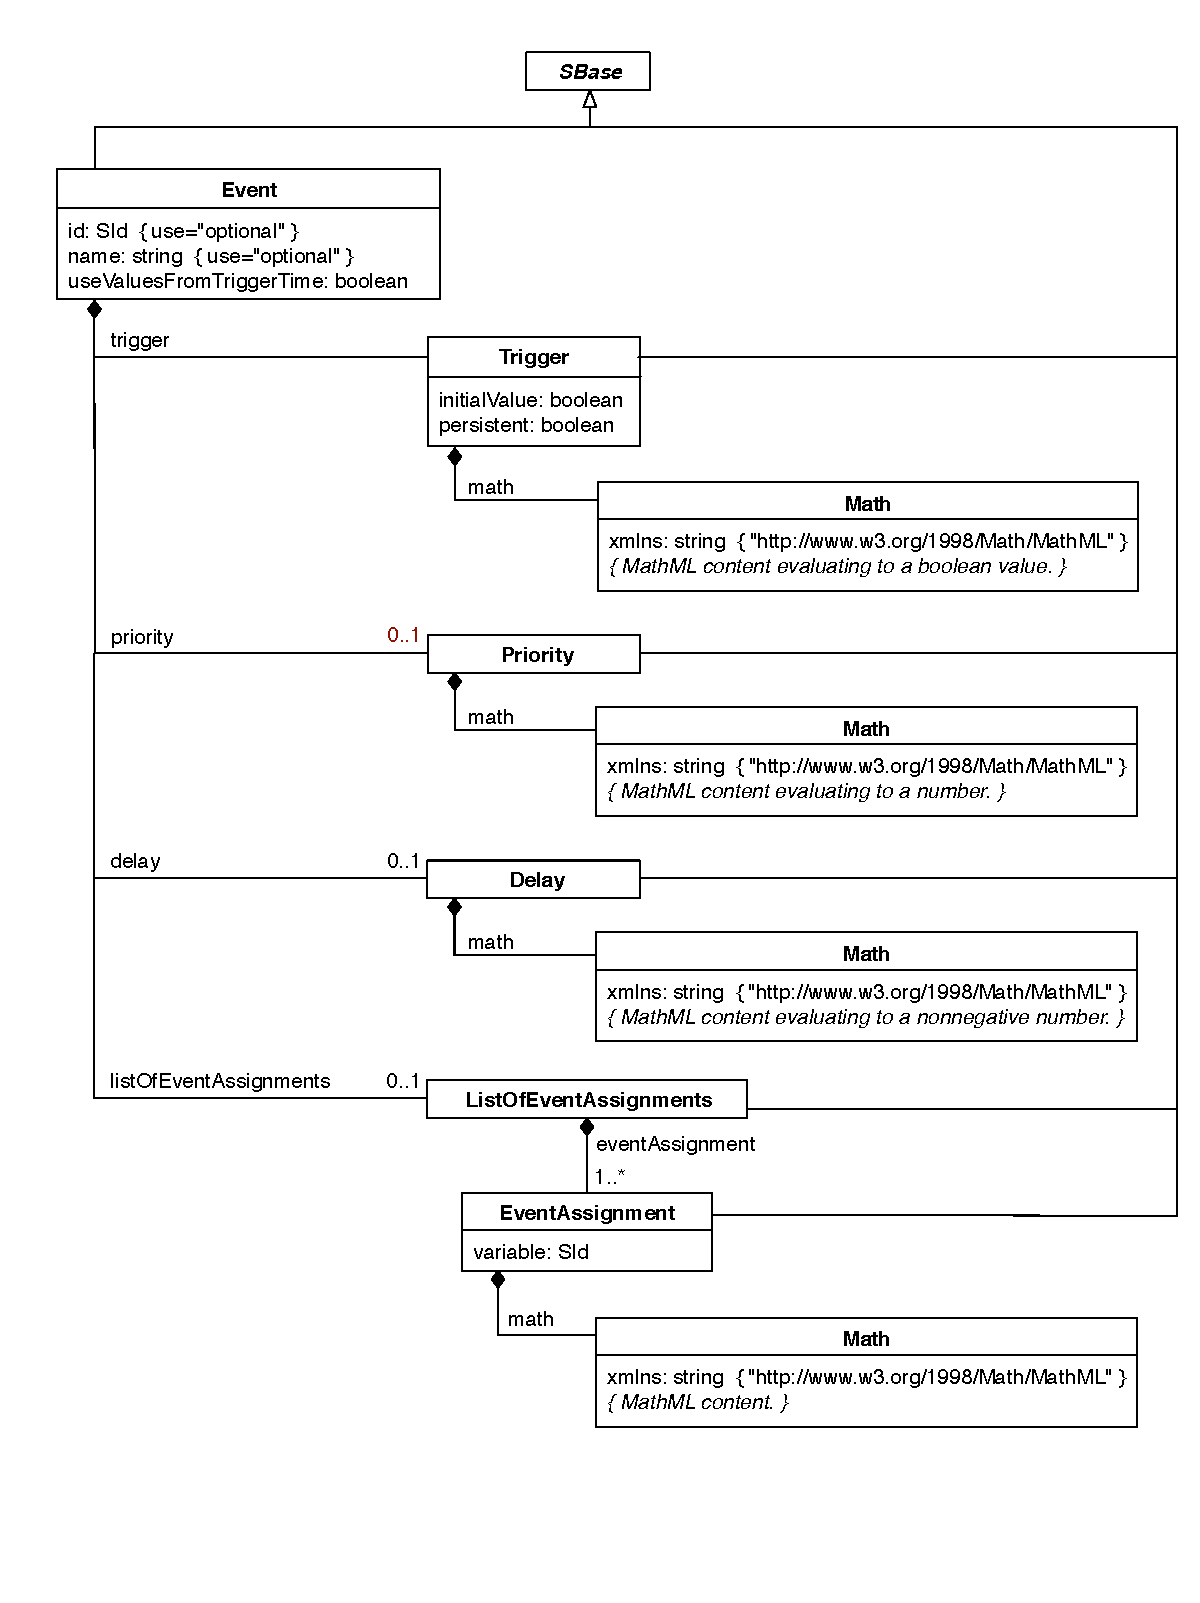
\includegraphics[scale=0.77]{figs/event-uml}
  \vspace*{-1ex}
  \caption{The definitions of \Event, \Trigger, \Delay, \Priority,
    \EventAssignment, and \ListOfEventAssignments.}
  \label{fig:event}
\end{figure}


\subsubsection{\class{Event}}

An \Event definition has one required attribute,
\token{useValuesFromTriggerTime}, and one required subobject, a
trigger condition in the form of \Trigger.  The remaining
components (the other attributes on \Event, and the subobjects
\Delay, \Priority, \ListOfEventAssignments, \EventAssignment) are
optional.  These various features of \Event are described below.


\paragraph{The \token{id} and \token{name} attributes}
\label{sec:event-id-name}

As with most components in SBML, an \Event has \token{id} and
\token{name} attributes, but in the case of \Event, both are optional.
These attributes operate in the manner described in
Section~\ref{sec:idnameattribs}.


\paragraph{The optional \token{sboTerm} attribute on \class{Event}}
\label{sec:event-sboterm}

\Event inherits an optional \token{sboTerm} attribute of type
\primtype{SBOTerm} from \SBase (see
Sections~\ref{sec:sboterm-type} and~\ref{sec:sboTerm}).  When this
attribute is present on a given \Event object instance, its value
should be an SBO identifier belonging to the branch for type
\Event indicated in Table~\ref{tab:sboterm-availability}.  The
relationship is of the form ``the event \emph{is-a} X'', where X
is the SBO term.  The term chosen should be the most precise
(narrow) one that captures the role of the event in the model.

As discussed in Section~\ref{sec:sboTerm}, SBO labels are optional
information on a model.  Applications are free to ignore
\token{sboTerm} values.  A model must be interpretable without the
benefit of SBO labels.


\paragraph{\textcolor{black}{The \token{useValuesFromTriggerTime} attribute}}
\label{sec:event-usevaluesfromtriggertime}

The possibility of defining an optional \Delay within \Event, and
the potential for multiple simultaneously-triggered events, means
there are two times to consider when interpreting an event: the
moment at which the event \emph{triggered}, and the moment at
which its assignments are \emph{executed}.  (If a \Delay subobject
is present, these moments are separated by simulation time.  If
multiple events are triggered simultaneously, these moments are
separated by the sequential execution of the event assignments.)
Similarly, it is also possible to distinguish between the moment at
which the mathematical expression of an \EventAssignment object is
evaluated, and the moment at which this value is assigned to the
entity referenced by the \EventAssignment's \token{variable}
attribute.  A model could intend the \EventAssignment expression
to be evaluated either at the moment the event is triggered, or at
the moment the event assignments are executed.  (In the former case,
a model interpreter would have to save the calculated values until
the moment of execution.)

The attribute \token{useValuesFromTriggerTime} allows a model to
indicate the moment at which the event's assignments are to be
evaluated.  A value of \val{true} indicates the values assignments
are to be computed at the moment the event is \emph{triggered}.
Conversely, \token{useValuesFromTriggerTime}=\val{false} means the
assignments are to be computed at the moment the event is
\emph{executed}.  The attribute has no default value.


\subsubsection{\class{Trigger}}
\label{sec:trigger}
\label{sec:event-trigger}

As shown in Figure~\ref{fig:event}, an \Event object must contain
exactly one object of class \Trigger.  This object in turn must
contain two attributes, \token{persistent} and
\token{initialValue}, as well as a MathML \token{math} element.
The expression in the \token{math} element must evaluate to a
value of type \primtype{boolean}.  The exact moment at which this
expression evaluates to \val{true} during a simulation is taken to
be the time point when the \Event is \emph{triggered}.

An event only triggers when the expression within its \Trigger object
makes the transition in value from \val{false} to \val{true}.  The
event will trigger again at any subsequent time points when the
trigger makes the transition from \val{false} to \val{true}; in
other words, an event can trigger multiple times during a simulation
if its trigger condition makes the transition from \val{false} to
\val{true} more than once.  The behavior at the very start of
simulation time (\ie $t = 0$, where $t$ stands for time) is
determined in part by the boolean flag
\token{initialValue}, discussed below.


\paragraph{The \token{persistent} attribute on \class{Trigger}}
\label{sec:trigger-persistent}

In the interval between when an \Event object \emph{triggers} (\ie
its \Trigger object expression transitions in value from
\val{false} to \val{true}) and when its assignments are to be
\emph{executed}, conditions in the model may change such that the
trigger expression transitions back from \val{true} to
\val{false}.  Should the event's assignments still be made if this
happens?  Answering this question is the purpose of the
\token{persistent} attribute on \Trigger.

If the boolean attribute \token{persistent} has a value of
\val{true}, then once the event is triggered, all of its assignments
are always performed when the time of execution is reached.  The
name ``persistent'' is meant to evoke the idea that the trigger
expression does not have to be re-checked after it triggers if
\token{persistent}=\val{true}.  Conversely, if the attribute value
is \val{false}, then the trigger expression is not assumed to
persist: if the expression transitions in value back to
\val{false} at any time between when the event triggered and when it
is to be executed, the event is no longer considered to have triggered
and its assignments are not executed.  (If the trigger expression
transitions once more to \val{true} after that point, then the
event is triggered, but this then constitutes a whole new event
trigger-and-execute sequence.)

The \token{persistent} attribute can be especially useful when
\Event objects contain \Delay objects, but it is relevant even in
a model without delays if the model contains two or more events.
As explained in the introduction to this section, the operation of
all events in SBML (delayed or not) is conceptually divided into
two phases, \emph{triggering} and \emph{execution}; however, unless
events have priorities associated with them (see
Section~\ref{sec:event-priority}), SBML does not mandate a
particular ordering of event execution in the case of simultaneous
events (see Section~\ref{sec:event-semantics}).  Models with
multiple events can lead to situations where the execution of one
event affects another event's trigger expression value.  If that
other event has \token{persistent}=\val{false}, and its trigger
expression evaluates to \val{false} before it is to be executed,
the event must not be executed after all.


\paragraph{The \token{initialValue} attribute on \Trigger}
\label{sec:trigger-initialvalue}

As mentioned above, an event \emph{triggers} when the mathematical
expression in its \Trigger object transitions in value from
\val{false} to \val{true}.  An unanswered question concerns what
happens at the start of a simulation: can event triggers make this
transition at $t = 0$, where $t$ stands for time?

In order to determine whether an event may trigger at $t = 0$, it is
necessary to know what value the \Trigger object's \token{math}
expression had immediately prior to $t = 0$.  This starting value
of the trigger expression is determined by the value of the
boolean attribute \token{initialValue}.  A value of \val{true}
means the trigger expression is taken to have the value \val{true}
immediately prior to $t = 0$.  In that case, the trigger cannot
transition in value from \val{false} to \val{true} at the moment
simulation begins (because it has the value \val{true} both before
and after $t = 0$), and can only make the transition from
\val{false} to \val{true} sometime \emph{after} $t = 0$.  (To do
that, it would also first have to transition to \val{false} before
it could make the transition from \val{false} back to \val{true}.)
Conversely, if \token{initialValue}=\val{false}, then the trigger
expression is assumed to start with the value \val{false}, and
therefore may trigger at $t = 0$ if the expression evaluates to
\val{true} at that moment.

% [2010-09-09 MH] I'm thinking we should leave this for a
% document explaining the differences between L2 and L3.
%
% We note in passing that in SBML Level~2, where \Trigger lacks the
% \token{initialValue} attribute, event triggers can never
% transition from \val{false} to \val{true} at precisely $t = 0$.
% In this respect, SBML Level~2 events are similar to Level~3
% events having \token{initialValue}=\val{true}.


\paragraph{The optional \token{sboTerm} attribute on \Trigger}
\label{sec:trigger-sboterm}

\Trigger inherits an optional \token{sboTerm} attribute of type
\primtype{SBOTerm} from its parent class \SBase (see
Sections~\ref{sec:sboterm-type} and~\ref{sec:sboTerm}).  The value
given to this attribute should be an SBO identifier belonging to
the branch for type \Trigger indicated in
Table~\ref{tab:sboterm-availability}.  The relationship is of the
form ``the trigger \emph{is-a} X'', where X is the SBO term.  The
term chosen should be the most precise (narrow) one that captures
the role of the trigger in the model.

As discussed in Section~\ref{sec:sboTerm}, SBO labels are optional
information on a model.  Applications are free to ignore
\token{sboTerm} values.  A model must be interpretable without the
benefit of SBO labels.

\subsubsection{\class{Priority}}
\label{sec:event-priority}

As shown in Figure~\ref{fig:event}, an \Event object can contain
an optional \Priority subobject.  The \Priority object class, like
\Delay, is derived from \SBase and contains a MathML formula
stored in the element \token{math}.  This formula is used to
compute a dimensionless numerical value that influences the order
in which a simulator is to perform the assignments of two or more
events that happen to be executed simultaneously.  The formula may
evaluate to any \token{double} value (and thus may be a positive
or negative number, or zero), with positive numbers taken to
signifying a higher priority than zero or negative numbers.  If no
\Priority object is present on a given \Event object, no priority
is defined for that event.


\paragraph{The interpretation of priorities on events in a model}

For the purposes of SBML, \emph{simultaneous event execution} is
defined as the situation in which multiple events have identical
times of execution.  The time of execution is calculated as the
sum of the time at which a given event's \Trigger is \emph{triggered}
plus its \Delay duration, if any.  Here, ``identical times'' means
\emph{mathematically equal} instants in time.  (In practice,
simulation software adhering to this specification may have to
rely on numerical equality instead of strict mathematical
equality; robust models will ensure that this difference will not
cause significant discrepancies from expected behavior.)

If no \Priority subobjects are defined for two or more \Event
objects, then those events are still executed simultaneously but
their order of execution is \emph{undefined by this SBML
  specification}.  A software implementation may choose to execute
such simultaneous events in any order, as long as each event is
executed only once and the requirements of checking the
\token{persistent} attribute (and acting accordingly) are
satisfied.  See Section~\ref{sec:trigger-persistent} for more
information about the attribute \token{persistent}.

If \Priority subobjects are defined for two or more
simultaneously-triggered events, the order in which those particular
events must be executed is dictated by their \Priority objects,
as follows.  If the values calculated using the two \Priority
objects' \token{math} expressions differ, then the event having
the higher priority value must be executed before the event with
the lower value.  If, instead, the two priority values are
mathematically equal, then the two events must be triggered in a
\emph{random} order.  It is important to note that a \emph{random
  order is not the same as an undefined order}: given multiple
runs of the same model with identical conditions, an undefined
ordering would permit a system to execute the events in (for
example) the same order every time (according to whatever scheme
may have been implemented by the system), whereas the explicit
requirement for random ordering means that the order of execution
in different simulation runs depends on random chance.  In other
words, given two events ``A'' and ``B'', a randomly-determined
order must lead to an equal chance of executing ``A'' first or
``B'' first, every time those two events are executed
simultaneously.

A model may contain a mixture of events, some of which have
\Priority subobjects and some do not.  Should a combination of
simultaneous events arise in which some events have priorities
defined and others do not, the set of events with defined
priorities must trigger in the order determined by their \Priority
objects, and the set of events without \Priority objects must be
executed in an \emph{undefined} order with respect to each other
and with respect to the events with \Priority subobjects.  (Note
that \emph{undefined order} does not necessarily mean random
order, although a random ordering would be a valid implementation
of this requirement.)

The following example may help further clarify these points.
Suppose a model contains four events that should be executed
simultaneously, with two of the events having \Priority objects
with the same value and the other two events having \Priority
objects with the same, but different, value.  The two events with
the higher priorities must be executed first, in a random order
with respect to each other, and the remaining two events must be
executed after them, again in a random order, for a total of four
possible and equally-likely event executions: A-B-C-D, A-B-D-C,
B-A-C-D, and B-A-D-C.  If, instead, the model contains four events
all having the same \Priority values, there are 4! or 24
possible orderings, each of which must be equally likely to be
chosen.  Finally, if none of the four events has a \Priority
subobject defined, or even if exactly one of the four events has a
defined \Priority, there are again 24 possible orderings, but the
likelihood of choosing any particular ordering is undefined; the
simulator can choose between events as it wishes.  (The SBML
specification only defines the effects of priorities on \Event
objects with respect to \emph{other} \Event objects with
priorities.  Putting a priority on a \emph{single} \Event object
in a model does not cause it to fall within that scope.)

Section~\ref{sec:event-semantics} includes additional discussion
of these topics.


\paragraph{Evaluation of \class{Priority} expressions}

An event's \Priority object \token{math} expression must be
evaluated at the time the \Event is to be \emph{executed}.  During
a simulation, all simultaneous events have their \Priority values
calculated, and the event with the highest priority is selected for
next execution.  Note that it is possible for the execution of one
\Event object to cause the \Priority value of another
simultaneously-executing \Event object to change (as well as to
trigger other events, as already noted).  Thus, after executing
one event, and checking whether any other events in the model have
been triggered, all remaining simultaneous events that
\emph{either} (i) have \Trigger objects with attributes
\token{persistent}=\val{false} \emph{or} (ii) have \Trigger
expressions that did not transition from \val{true} to
\val{false}, must have their \Priority expression reevaluated.
The highest-priority remaining event must then be selected for 
execution next.  Section~\ref{sec:bp:events} provides further
discussion about implementing support for events.


\paragraph{Units of \class{Priority} object's mathematical
  expressions}

The unit associated with the value of a \Priority object's
\token{math} expression should be \token{dimensionless}.  This is
because the priority expression only serves to provide a relative
ordering between different events, and only has meaning with
respect to other \Priority object expressions.  The value of
\Priority objects is not comparable to any other kind of object in
an SBML model.


\paragraph{The optional \token{sboTerm} attribute on \class{Priority}}
\label{sec:priority-sboterm}

\Priority inherits an optional \token{sboTerm} attribute of type
\primtype{SBOTerm} from its parent class \SBase (see
Sections~\ref{sec:sboterm-type} and~\ref{sec:sboTerm}).  When a
value is given to this attribute in a \Priority instance, it
should be an SBO identifier belonging to the branch for type
\Priority indicated in Table~\ref{tab:sboterm-availability}.  The
relationship is of the form ``the priority \emph{is-a} X'', where
X is the SBO term.  The term chosen should be the most precise
(narrow) one that captures the role of the priority in the model.

As discussed in Section~\ref{sec:sboTerm}, SBO labels are optional
information on a model.  Applications are free to ignore
\token{sboTerm} values.  A model must be interpretable without the
benefit of SBO labels.


\subsubsection{\class{Delay}}
\label{sec:event-delay}

As shown in Figure~\ref{fig:event}, an \Event object can contain
an optional \Delay object.  The \Delay class is derived from
\SBase and contains a mathematical formula stored in \token{math}.
The formula is used to compute the length of time between when the
event has \emph{triggered} and when the event's assignments (see
below) are actually \emph{executed}.  If no delay is present on a
given \Event, no delay is defined for that event.

The expression in the \Delay object's \token{math} element must be
evaluated at the time the event is \emph{triggered}.  The expression
must always evaluate to a nonnegative number (otherwise, a
nonsensical situation could arise where an event is defined to
execute before it is triggered!).


\paragraph{Units of delay expressions}

The unit associated with the value of a \Delay object's
\token{math} expression should match the model's unit of
\quantity{time} (see Section~\ref{sec:model-timeUnits}).  Note
that, as in other cases of MathML expressions in SBML, units are
\emph{not} automatically predefined or assumed.  As discussed in
Section~\ref{sec:operator-arg-types}, expressions containing only
literal numbers and/or \Parameter objects without declared units
are considered to have unspecified units.  In such cases, the
correspondence between the needed entity units and the (unknown)
unit for the \Delay's \token{math} expression cannot be proven,
and while such expressions are not considered inconsistent, all
that can be assumed by model interpreters (whether software or
human) is that the units \emph{may} be consistent.

The following \Event example fragment helps illustrate this:
\label{sec:event:delay:example}

\vspace*{0.5ex}
\begin{example}
<model timeUnits="second" ...>
    ...
    <listOfEvents>
        <event useValuesFromTriggerTime="true">
            ...
            <delay>
                <math xmlns="http://www.w3.org/1998/Math/MathML">
                    <cn> 10 </cn>
                </math>
            </delay>
            ...
        </event>
    </listOfEvents>
    ...
</model>
\end{example}
\vspace*{0.5ex}

Note that the \val{<cn> 10 </cn>} within the mathematical formula
has no specified unit attached to it.  The model is not invalid
because of this, but a recipient of the model may justifiably be
concerned about what \val{10} really means.  (Ten seconds?  What
if the global unit of time on the model were changed from seconds
to milliseconds?  Would the modeler remember to change \val{10} to
\val{10$\;$000}?)  A better approach would be to declare the unit
explicitly, as in the following example:

\vspace*{0.5ex}
\begin{example}
<model timeUnits="second" ...>
    ...
    <listOfEvents>
        <event useValuesFromTriggerTime="true">
            ...
            <delay>
                <math xmlns="http://www.w3.org/1998/Math/MathML"
                      xmlns:sbml="http://www.sbml.org/sbml/level3/version1/core">
                    <cn sbml:units="second"> 10 </cn>
                </math>
            </delay>
            ...
        </event>
    </listOfEvents>
    ...
</model>
\end{example}
\vspace*{0.5ex}

While this approach will not solve the problem of updating the
value if the model's global of unit of time is changed, it will at
least inform readers of the intended duration of the delay itself
as well as make it possible for software tools to potentially
detect unit inconsistencies if the tools can perform unit
analysis.

Another, different approach is to define a global \Parameter
object for the time delay (with an appropriate unit attached), and
to replace the \token{cn} element above with a \token{ci} element
containing the parameter's identifier.  This has advantages
because \Parameter objects can have annotations and SBO terms
associated with them.


\paragraph{The optional \token{sboTerm} attribute on \class{Delay}}
\label{sec:delay-sboterm}

\Delay inherits an optional \token{sboTerm} attribute of type
\primtype{SBOTerm} from its parent class \SBase (see
Sections~\ref{sec:sboterm-type} and~\ref{sec:sboTerm}).  When a
value is given to this attribute in a \Delay instance, it should
be an SBO identifier belonging to the branch for type \Delay
indicated in Table~\ref{tab:sboterm-availability}.  The
relationship is of the form ``the delay \emph{is-a} X'', where X
is the SBO term.  The term chosen should be the most precise
(narrow) one that captures the role of the delay in the model.

As discussed in Section~\ref{sec:sboTerm}, SBO labels are optional
information on a model.  Applications are free to ignore
\token{sboTerm} values.  A model must be interpretable without the
benefit of SBO labels.


\subsubsection{\class{EventAssignment}}
\label{sec:eventassignment}
\label{sec:listofeventassignments}

\Event contains an optional element called
\token{listOfEventAssignments}, of class \ListOfEventAssignments.
In every instance of an event definition in a model, the object's
\token{listOfEventAssignments} element must have a non-empty list
of one or more \token{eventAssignment} elements of class
\EventAssignment.  The object class \EventAssignment has one
required attribute, \token{variable}, and a required element,
\token{math}.  Being derived from \SBase, it also has all the
usual attributes and elements of its parent class.

An ``event assignment'' has effect when the event is
\emph{executed}.  (As noted above, the operation of event is
divided conceptually into two phases: the first phase when the
event is \emph{triggered} and the second phase when the event is
\emph{executed}.)  See Section~\ref{sec:event-semantics} below for
more information about events and event assignments.


\paragraph{The \token{variable} attribute}

The \Event attribute \token{variable} has type
\primtype{SIdRef} and can contain the identifier of a
\Compartment, \Species, \SpeciesReference, or \Parameter instance
defined in the model.  When the event is executed, the value of
the model component identified by \token{variable} is changed by
the \EventAssignment to the value computed by the \token{math}
element; that is, a species' quantity, species reference's
stoichiometry, compartment's size or parameter's value are reset
to the value computed by \token{math}.

Certain restrictions are placed on what can appear in
\token{variable}:
\begin{itemize}
  
\item The object identified by the value of the \token{variable}
  attribute must not have its \token{constant} attribute set 
  to \val{true}.  (Constants cannot be affected by events.)
  
\item The \token{variable} attribute must not contain the
  identifier of a reaction; only species, species references,
  compartment and parameter values may be set by an \Event.
  
\item The value of every \token{variable} attribute must be unique
  among the set of \EventAssignment objects within a given
  \Event instance.  In other words, a single event cannot have
  multiple \EventAssignment{}s assigning the same variable.  (All
  of them would be performed at the same time, when that
  particular \Event triggers, resulting in indeterminacy.)
  Separate \Event instances can refer to the same variable.
  
\item A variable cannot be assigned a value in an \EventAssignment
  object instance and also be assigned a value by an
  \AssignmentRule, \ie the value of the \token{variable} attribute
  in an \EventAssignment instance cannot be the same as the value
  of a \token{variable} attribute in an \AssignmentRule instance.
  (Assignment rules hold at all times, therefore it would be
  inconsistent to also define an event that reassigns the value of
  the same variable.)

\end{itemize}

Note that the time of assignment of the object identified by the
value of \token{variable} is always the time at which the \Event
is \emph{executed}, not when it is \emph{triggered}.  The timing
is controlled by the optional \Delay.  The time of assignment is
not affected by the \Event attribute
\token{useValuesFromTriggerTime}---that attribute affects the time
at which the \EventAssignment's \token{math} expression is
evaluated.  In other words, SBML allows decoupling the time at
which the \token{variable} is assigned from the time at which its
value expression is calculated.


\paragraph{The optional \token{sboTerm} attribute on \class{EventAssignment}}
\label{sec:eventassignment-sboterm}

\EventAssignment   inherits an optional \token{sboTerm}
attribute of type \primtype{SBOTerm} from its parent
class \SBase (see Sections~\ref{sec:sboterm-type}
and~\ref{sec:sboTerm}).  When a value is given to this
attribute in a  \EventAssignment  instance, it should be an
SBO identifier belonging to the branch for type  \EventAssignment 
indicated in Table~\ref{tab:sboterm-availability}.  The relationship is
of the form ``the event assignment \emph{is-a} X'', where X is
the SBO term.  The term chosen should be the most precise (narrow)
one that captures the role of the event assignment  in the model.

As discussed in Section~\ref{sec:sboTerm}, SBO labels are optional
information on a model.  Applications are free to ignore
\token{sboTerm} values.  A model must be interpretable without the
benefit of SBO labels.


\paragraph{\class{EventAssignment}'s \token{math}}

The \token{math} element contains a MathML expression that defines
the new value to be given to the object identified by the
\EventAssignment attribute \token{variable}.

As mentioned above, the time at which the expression in
\token{math} is evaluated is determined by the attribute
\token{useValuesFromTriggerTime} on \Event.  If the attribute
value is \val{true}, the expression must be evaluated when the
event is \emph{triggered}; more precisely, the values of identifiers
occurring in MathML \token{ci} attributes in the
\EventAssignment's \token{math} expression are the values they
have at the point when the event \emph{triggered}.  If, instead,
\token{useValuesFromTriggerTime}'s value is \val{false}, it means
the values at \emph{execution} time should be used; that is, the
values of identifiers occurring in MathML \token{ci} attributes in
the \EventAssignment's \token{math} expression are the values they
have at the point when the event \emph{executed}.


\paragraph{Units of the \token{math} formula in \class{EventAssignment}}

In all cases, as would be expected, the unit of measurement
associated with value of the formula contained in the \token{math}
element of an \EventAssignment object should be consistent with
the unit associated with the object identified by the
\token{variable} attribute value.  More precisely:
\begin{itemize}
  
\item \emph{In the case of a species}, an \EventAssignment sets
  the referenced species' quantity (\quantity{concentration} or
  \quantity{amount}) to the value determined by the formula in
  \token{math}.  The unit associated with the value produced by
  the \token{math} formula should be equal to the unit associated
  with the species' quantity.  (See
  Section~\ref{sec:species-units} for an explanation of how a
  species' quantity is determined.)

\item \emph{In the case of a species reference}, an
  \EventAssignment sets the stoichiometry of the reactant or
  product referenced by the \SpeciesReference object to the value
  determined by the formula in \token{math}.  The unit associated
  with the value produced by the \token{math} formula should be
  \token{dimensionless}, because reactant and product
  stoichiometries in reactions are dimensionless quantities.

\item \emph{In the case of a compartment}, an \EventAssignment
  sets the referenced compartment's size to the size determined by
  the formula in \token{math}.  The unit associated with the value
  produced by the \token{math} formula should be the same as that
  specified for the compartment's size.  (See
  Section~\ref{sec:compartment-units} for more.)

\item \emph{In the case of a parameter}, an \EventAssignment sets
  the parameter's value to the value of the formula in
  \token{math}.  The unit associated with the value produced by
  the \token{math} formula should be the same as parameter's
  \token{units} attribute value.
  (Section~\ref{sec:parameter-units} for more information about
  parameter units.)

\end{itemize}

Note that the formula in \token{math} has no assumed unit of
measurement associated with it.  The consistency of the units
between the formula and the entity affected by the assignment
should be established explicitly.

% \todo{someone}{explain what to do if event sets both species
% and a compartment size at same time}


\subsubsection{Example \class{Event} definitions}

The following is an example of an event.  This structure makes the
assignment $k_2 = 0$ when $P_1 \leq P_2$:

\begin{example}
<model>
    ...
    <listOfUnitDefinitions>
        <unitDefinition id="per_second">
            <listOfUnits>
                <unit kind="second" exponent="-1" multiplier="1" scale="0"/>
            </listOfUnits>
        </unitDefinition>
    </listOfUnitDefinitions>
    ...
    <listOfParameters>
        <parameter id="k2" value="0.05" units="per_second" constant="false"/>
        <parameter id="k2reset" value="0.0" units="per_second" constant="true"/>
    </listOfParameters>
    ...
    <listOfEvents>
        <event useValuesFromTriggerTime="true">
            <trigger initialValue="false" persistent="true">
                <math xmlns="http://www.w3.org/1998/Math/MathML">
                    <apply> <leq/> <ci> P_1 </ci> <ci> P_2 </ci> </apply>
                </math>
            </trigger>
            <listOfEventAssignments>
                <eventAssignment variable="k2">
                    <math xmlns="http://www.w3.org/1998/Math/MathML">
                        <ci> k2reset </ci>
                    </math>
                </eventAssignment>
            <listOfEventAssignments>
        </event>
    </listOfEvents>
</model>
\end{example}

A complete example of a model using events is given in
Section~\ref{sec:eventeg}.


\subsubsection{Detailed semantics of events}
\label{sec:event-semantics}

Any transition of a \Trigger object's \token{math} formula from
the value \val{false} to \val{true} will cause the enclosing
\Event object to \emph{trigger}.  Such a transition is not possible
at the very start of a simulation (\ie at time $t = 0$) unless the
\Trigger object's \token{initialValue} attribute has a value of
\val{false}; this defines the value of the trigger formula to be
\val{false} immediately prior to the start of simulation, thereby
giving it the potential to change in value from \val{false} to
\val{true} when the formula is evaluated at $t = 0$.  If
\token{initialValue}=\val{true}, then the trigger expression
cannot transition from \val{false} to \val{true} at $t = 0$ but
may do so at some time $t > 0$.

Consider an \Event object definition $E$ with delay $d$ in which
the \Trigger object's \token{math} formula makes a transition in
value from \val{false} to \val{true} at times $t_1$ and $t_2$.
The \EventAssignment within the \Event object will have effect at
$t_1+d$ and $t_2+d$ irrespective of the relative times of $t_1$
and $t_2$.  For example, events can ``overlap'' so that $t_1 < t_2
< t_1+d$ still causes an event assignments to occur at $t_1+d$ and
$t_2+d$.

It is entirely possible for two events to be executed
simultaneously, and it is possible for events to trigger other events
(\ie an event assignment can cause an event to trigger).  This leads
to several points:
\begin{itemize}

\item A software package should retest all event triggers after
  executing an event assignment in order to account for the
  possibility that the assignment causes another event trigger to
  transition from \val{false} to \val{true}.  This check should be
  made after each individual \Event object's execution, even when
  several events are to be executed simultaneously.  

\item Any \Event object whose \Trigger \token{persistent}
  attribute has the value \val{false} must have its trigger
  expression reevaluated continuously between when the event has
  been triggered and when it is executed.  If its trigger expression
  ever evaluates to \val{false}, it must be removed from the queue
  of events pending execution and treated as any other event whose
  trigger expression evaluates to \val{false}.

\item Although the precise time at which events are executed is
  not resolved beyond the given execution point in simulated time,
  it is assumed that the order in which the events occur \emph{is}
  resolved.  This order can be significant in determining the
  overall outcome of a given simulation.  When an event $X$
  \emph{triggers} another event $Y$ and event $Y$ has zero delay,
  then event $Y$ is added to the existing set of simultaneous
  events that are pending \emph{execution}.  Events $X$ and $Y$
  form a cascade of events at the same point in simulation time.
  An event such as $Y$ may have a special priority if it contains
  a \Priority subobject.

\item All events in a model are open to being in a cascade.  The
  position of an event in the event queue does not affect whether
  it can be in the cascade: event $Y$ can be triggered whether it
  is before or after $X$ in the queue of events pending execution.
  A cascade of events can be potentially infinite (never
  terminate); when this occurs a simulator should indicate this
  has occurred---it is incorrect for a simulator to break a
  cascade arbitrarily and continue the simulation without at least
  indicating that the infinite cascade occurred.

\item Simultaneous events having no defined priorities are
  executed in an undefined order.  This does not mean that the
  behavior of the simulation is completely undefined; merely that
  the \emph{order} of execution of these particular events is
  undefined.  A given simulator may use any algorithm to choose an
  order as long as every event is executed exactly once.  (See
  also Section~\ref{sec:event-priority}.)

\item Events with defined priorities are executed in the order
  implied by their \Priority \token{math} formula values, with
  events having higher priorities being executed ahead of events
  with lower priorities, and events with identical priorities
  being executed in a random order with respect to one another (as
  determined at run-time by some random algorithm equivalent to
  coin-flipping).  Newly-triggered events that are to be executed
  immediately (\ie if they define no delays) should be inserted
  into the queue of events pending execution according to their
  priorities: events with higher priority values value must be
  inserted ahead of events with lower priority values and after
  any pending events with even higher priorities, and inserted
  randomly among pending events with the same priority values.
  Events without \Priority objects must be inserted into the queue
  in some fashion, but the algorithm used to place it in the queue
  is undefined.  Similarly, there is no restriction on the order
  of a newly-inserted event with a defined \Priority with respect
  to any other pending \Event without a defined \Priority.  (See
  Section~\ref{sec:event-priority}.)

% [2010-09-09 MH] I don't think the following point is necessary.
% 
% \item Any event that has been executed is part of the history of
%   the model, and not part of the current state of the model.  (For
%   example, if the execution of an event with a low priority value
%   causes a different event with a higher priority to trigger and
%   immedately be executed, it is not a problem that a
%   lower-priority event executed before a higher-priority event.)

\item A model variable that is the target of one or more event
  assignments can change more than once when simultaneous events
  are processed at some time point $t$.  The model's behavior
  (output) for such a variable is the value of the variable at the
  end of processing all the simultaneous events at time $t$.

\end{itemize}


% -----------------------------------------------------------------------------
% chunks of text that maybe will be useful some day:
% -----------------------------------------------------------------------------

% Here it pays to reflect more carefully about what a reaction is.
% A reaction represents a process occurring over time.  the process
% acts on the reactants, transforming them in some way into the
% products.  the transformation may be anything from a change in
% the nature of the reactants to a simple relocation without any
% change to the nature of the reactants; for the purpose of talking
% about the speed of the reaction it does not matter.

% The ``kinetic law'' is a statement about the speed at which the
% process takes place, or more precisely, the frequency of the
% events occurring in this process.  It is by default in terms of
% moles per second, which has some intuitive appeal when dealing
% with chemical substances.  But notice that a ``mole'' is actually
% a statement about numbers of ``things'': it is 6.02e23 of whatever
% is involved.  In the case of chemical species, it is molecules of
% the substance.  To say ``one mole of'' is a shorthand way of
% saying ``6.02e23 molecules of''.  Thus, a reaction expressed as
% ``X moles per second'' is a statement that the process involves
% ``(X times 6.02e23) items per second''.

% 1 kg/sec is 1 kg/sec

% If in a reaction, the units of the species are the same as the
% reaction's substance units (default mole, redefinable by
% redefining ``substance''; sec section x), then the stoichiometries
% represent simply the ratios of the participating species: 1 mole
% of this to 2 moles of that, and so on.  If instead the species are
% given in different units, then the species quantities must be
% converted to be consistent with the units of the reaction.  Thus,
% the SBML stoichiometry may then have to incorporate a conversion:
% the stoichiometry will represent the product of the biochemical
% reaction stoichiometry and a ratio between the species substance
% and the reaction substance.

% don't forget units of reaction id


% ---

% started trying to generate the event diagram in pgf but
% it's too hard.

%   \begin{tikzpicture}[level distance=2in]
%     \node[left=1.15in,above=0.35in] (a) { \emptyClassbox{\textsl{SBase}} };
%     \node[left=0.75in] (b) {
%       \begin{classbox}{Event}
%         id: SId  \{ use="optional" \}     \\
%         name: string \{ use="optional" \} \\
%       \end{classbox} 
%     }
%     [diamond-,edge from parent fork right,grow=right,sibling distance=0.6in]
%     child {node[right=0.15in] (c) { \emptyClassbox{ListOfEventAssignments} }
%       child {node (f) {
%           \begin{classbox}{EventAssignment}
%             variable: SIdRef                                                   \\
%           \end{classbox}
%         }}
%       child {node (g) {
%           \begin{classbox}{Math}
%             xmlns: string \{ "http://www.w3.org/1998/Math/MathML" \} \\
%             \{ \emph{\mathml content} \} \\
%           \end{classbox}
%         }}
%     }
%     child {node[right=0.15in] (d) { \emptyClassbox{Delay} }
%     }
%     child {node[right=0.15in] (d) { \emptyClassbox{Trigger} }
%     }
      
% junk

%      [diamond-,edge from parent fork down,sibling distance=0.6in]
%         \begin{classbox}{Delay}
%           xmlns: string \{ "http://www.w3.org/1998/Math/MathML" \} \\
%           \{ \emph{\mathml content} \} \\
%         \end{classbox}
%       }}
%     child {node[right=0.15in] (e) {
%         \begin{classbox}{Trigger}
%           xmlns: string \{ "http://www.w3.org/1998/Math/MathML" \} \\
%           \{ \emph{\mathml content evaluating to a boolean value} \} \\
%         \end{classbox}
%       }}
%    ;
%           \begin{classbox}{EventAssignment}
%             variable: SIdRef                                                   \\
%             math: Math \{ namespace="http://www.w3.org/1998/Math/MathML" \} \\
%           \end{classbox}
%      \draw[open triangle 60-] (a) -- (b);
%      \draw node[left=0.4in,above=0.375in] {\textsf{math}};
%      \draw node[left=0.3in,below=0.225in] {\textsf{message}};
%      \draw node[left=-0.15in,below=0.215in] {\textsf{0..1}};
%  \end{tikzpicture}

%   
%   \vspace*{2ex}
%   \begin{classbox}{Trigger}
%     math: Math \{ namespace="http://www.w3.org/1998/Math/MathML" \} \\
%   \end{classbox}
%   \vspace*{2ex}
%   \begin{classbox}{Delay}
%     math: Math \{ namespace="http://www.w3.org/1998/Math/MathML" \} \\
%   \end{classbox}
%   \vspace*{2ex}
%   

% -*- TeX-master: "sbml-level-3-version-2-core"; fill-column: 66 -*-
% ----------------------------------------------------------------

\section{The Systems Biology Ontology and the \tokenNC{sboTerm} attribute}
\label{sec:sboTerm}
\label{sec:sbo}

The values of \token{id} attributes on SBML components allow the
components to be cross-referenced within a model. The values of
\token{name} attributes on SBML components provide the opportunity
to assign them meaningful labels suitable for display to humans
(\sec{sec:idnameattribs}).  The specific identifiers and
labels used in a model necessarily must be unrestricted by SBML,
so that software and users are free to pick whatever they need.
However, this freedom makes it more difficult for software tools
to determine, without additional human intervention, the semantics
of models more precisely than the semantics provided by the SBML
object classes defined in other sections of this document.  For
example, there is nothing inherent in a parameter with identifier
``\token{k}'' that would indicate to a software tool it is a
first-order rate constant (if that's what ``\token{k}'' happened
to be in some given model).  However, one may need to convert a
model between different representations (\eg
Henri-Michaelis-Menten vs.\ elementary steps), or to use it with
different modeling approaches (discrete or continuous).  One may
also need to relate the model components with other description
formats such as SBGN (\url{http://www.sbgn.org/}) using deeper
semantics.  Although an advanced software tool \emph{might} be
able to deduce the semantics of some model components through
detailed analysis of the kinetic rate expressions and other parts
of the model, this quickly becomes infeasible for any but the
simplest of models.

An approach to solving this problem is to associate model
components with terms from carefully curated controlled
vocabularies (CVs).  This is the purpose of the optional
\token{sboTerm} attribute provided on the SBML
class \SBase.  The \token{sboTerm} attribute always refers to
terms belonging to the Systems Biology Ontology (SBO, \citep{courtot:2011}). In
this section, we discuss the \token{sboTerm} attribute,
SBO, the motivations and theory behind their introduction, and
guidelines for their use.

SBO is not part of SBML; it is being developed separately, to
allow the modeling community to evolve the ontology independently
of SBML.  However, the terms in the ontology are being designed
keeping SBML components in mind, and are classified into subsets that
can be directly related with SBML components such as reaction rate
expressions, parameters, and a few others, see below.  The use of
\token{sboTerm} attributes is optional, and the presence of
\token{sboTerm} on an element does not change the way the model is
\emph{interpreted}.  Annotating SBML elements with SBO terms
adds additional semantic information that may be used to
\emph{convert} the model into another model, or another format.
Although SBO support provides an important source of information to
understand the meaning of a model, software does not need to
support \token{sboTerm} to be considered SBML-compliant.

\subsection{Principles}
\label{sec:sbo-principles}

Labeling model components with terms from shared controlled
vocabularies allows a software tool to identify each component using
identifiers that are not tool-specific.  An example of where this
is useful is the desire by many software developers to provide
users with meaningful names for reaction rate equations.  Software
tools with editing interfaces frequently provide these names
in menus or lists of choices for users.  However, without a
standardized set of names or identifiers shared between
developers, a given software package cannot reliably interpret the
names or identifiers of reactions used in models written
by other tools.

The first solution that might come to mind is to stipulate that
certain common reactions always have the same name (\eg
``Michaelis-Menten''), but this is simply impossible to do: not
only do humans often disagree on the names themselves, but it
would not allow for correction of errors or updates to the list of
predefined names except by issuing new releases of the SBML
specification---to say nothing of many other limitations with this
approach.  Moreover, the parameters and variables that appear in
rate expressions also need to be identified in a way that software
tools can interpret mechanically, implying that the names of these
entities would also need to be regulated.

The Systems Biology Ontology provides terms for identifying
most elements of SBML.  The relationship implied by an
\token{sboTerm} on an SBML model component is ``is-a'' between the
characteristic of the component meant to be described by SBO on
this element and the SBO term identified by the value of the
\token{sboTerm}.  By adding SBO term references on the components
of a model, a software tool can provide additional details using
shared vocabularies that can enable \emph{other} software tools to
recognize precisely what the component is meant to be.  Those
tools can then act on that information.  For example, if the SBO
identifier \token{SBO:0000049} is assigned to the concept of
``first-order irreversible mass-action kinetics, continuous
framework'', and a given \KineticLaw object in a model has an
\token{sboTerm} attribute with this value, then regardless of the
identifier and name given to the reaction itself, a software tool
could use this to inform users that the reaction is a first-order
irreversible mass-action reaction.  This kind of reverse
engineering of the meaning of reactions in a model would be
difficult to do otherwise, especially for more complex reaction
types.

The presence of SBO labels on \Compartment, \Species, and
\Reaction objects in SBML can help map those entities to
equivalent concepts in other standards, such as (but not limited
to) BioPAX (\url{http://www.biopax.org/}), PSI-MI
(\url{http://www.psidev.info/index.php?q=node/60}), or the Systems
Biology Graphical Notation (SBGN, \url{http://www.sbgn.org/}).
Such mappings can be used in conversion procedures, or to build
interfaces, with SBO becoming a kind of ``glue'' between standards
of representation.

The presence of the label on a kinetic expression can also allow
software tools to make more intelligent decisions about reaction
rate expressions.  For example, an application could recognize
certain types of reaction formulas as being ones it
knows how to solve with optimized procedures.  The application
could then use internal, optimized code implementing the rate
formula indexed by identifiers such as \token{SBO:0000049}
(``mass action rate law for first order irreversible reactions,
continuous scheme'') appearing in SBML models.

Finally, SBO labels may be very valuable when it comes to model
integration, by helping identify interfaces, convert mathematical
expressions and parameters etc.

Although the use of SBO can be beneficial, it is critical to keep
in mind that the presence of an \token{sboTerm} value on an object
\emph{must not change the fundamental mathematical meaning} of the
model.  An SBML model must be defined such that it stands on its
own and does not depend on additional information added by SBO
terms for a correct mathematical interpretation.  SBO term
definitions will not imply any alternative mathematical semantics
for any SBML object labeled with that term.  Two important
reasons motivate this principle.  First, it would be too limiting
to require all software tools to be able to understand the SBO
vocabularies in addition to understanding SBML.
Supporting SBO is not only additional work for the software
developer; for some kinds of applications, it may not make sense.
If SBO terms on a model are optional, it follows that the SBML
model \emph{must} remain unambiguous and fully interpretable
without them, because an application reading the model may ignore
the terms.  Second, we believe allowing the use of \token{sboTerm}
to alter the mathematical meaning of a model would allow
  too much leeway to shoehorn inconsistent concepts into SBML
objects, ultimately reducing the interoperability of the
models.

\subsection{Using SBO and \tokenNC{sboTerm}}

The \token{sboTerm} attribute data type is always
\primtype{SBOTerm}, defined in \sec{sec:sboterm-type}.
When present in a given model object instance, the
attribute's value must be an identifier \changed{that refers}
to a single SBO term that best defines the entity encoded by
the SBML object in question.  An example of the type of
relationship intended is: \emph{the KineticLaw in reaction R1 is a
  first-order irreversible mass action rate law}.

Note the careful use of the words ``defines'' and ``entity encoded
by the SBML object'' in the paragraph above.  As mentioned, the
relationship between the SBML object and the URI is:

\begin{quote}
  The ``thing'' encoded by this SBML object has a characteristic
  that is an instance of the ``thing'' represented by the
  referenced SBO term.
\end{quote}

The characteristic relevant for each SBML object is described in
the second column of \tab{tab:sboterm-availability}.


\subsubsection{The structure of the Systems Biology Ontology}

The goal of SBO labeling for SBML is to clarify to the fullest
possible extent the nature of each element in a model.  The
approach taken in the Systems Biology Ontology begins with a
hierarchically-structured set of controlled vocabularies with \changed{seven}
main divisions: (1) \changed{physical} entity \changed{representation}, (2) participant role, (3) \changed{systems description} parameter, (4) modeling framework, (5)
mathematical expression, (6) \changed{occurring entity representation}, \changed{and (7) metadata representation}.  \fig{fig:sbo-top-level} illustrates
the highest level of SBO.

Each of the \changed{seven} branches of \fig{fig:sbo-top-level} has a
hierarchy of terms underneath them.  At this time, we can only
begin to list some initial concepts and terms in SBO; what follows
is not meant to be complete, comprehensive or even necessarily
consistent with future versions of SBO.  The web site for SBO
(\sboref) should be consulted for the current version of the
ontology.  \sec{sec:sbo-frequency-of-change} describes how
the impact of SBO changes on software applications is minimized.

\begin{figure}[tbh]
  \centering
  
\includegraphics[scale = 0.8]{figs/sbo-top-level}
  \vspace*{1ex}
  \caption{The six controlled vocabularies (CVs) that
      make up the main branches of SBO.}
  \label{fig:sbo-top-level}
\end{figure}

\fig{fig:expanded-species} shows the structure for the
\emph{\changed{physical} entity \changed{representation}} branch, which reflects the hierarchical groupings of
the types of entities that can be represented by a \Compartment or
\Species object.  Note that the values taken by the
\token{sboTerm} attribute on those elements should refer to SBO
terms belonging to the \emph{material entity} branch, so as to
distinguish whether the element represents a macromolecule, a
simple chemical, etc.  Indeed, this information remains valid for
the whole model. The term should not belong to the
\emph{functional entity} branch, representing the function of the
entity within a certain functional context. If one wants to use
this information, one should refer to the SBO terms using a
controlled RDF annotation instead
(\sec{sec:annotation-standard}), carefully choosing the
qualifiers (\sec{sec:qualified-dc-annotation}) to reflect
the fact that a given \Species object, for instance, can fulfill
different functions within a given model (\eg EGF receptor is a
receptor and an enzyme).

\begin{figure}[htb]
  \centering
  \vspace*{-1ex}
  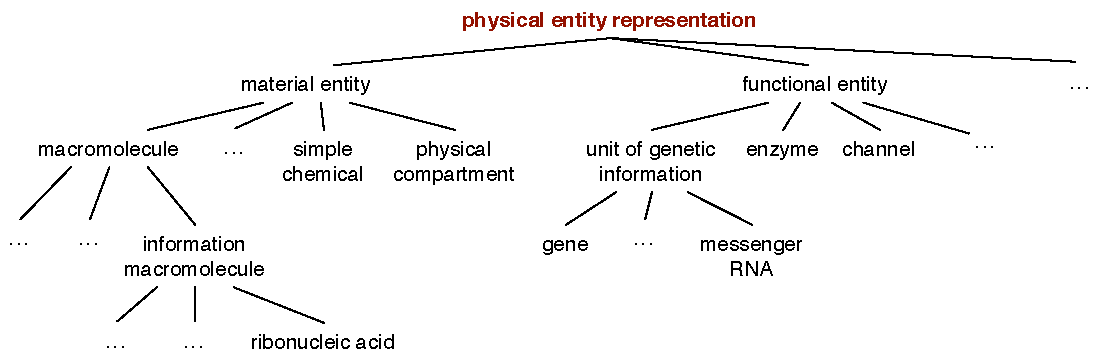
\includegraphics[scale = 0.78]{figs/sbo-entity}
  \caption{Partial expansion of some of the terms in the
    \emph{entity} branch of SBO.}
  \label{fig:expanded-species}
\end{figure}

\fig{fig:expanded-speciesRef} shows the structure for the
\emph{participant role} branch, also grouping the concepts in a
hierarchical manner.  For example, in reaction rate expressions,
there are a variety of possible modifiers.  Some classes of
modifiers can be further subdivided and grouped.  All of this is
easy to capture in the ontology.  As more agreement is reached in
the modeling community about how to define and name modifiers for
different cases, the ontology can grow to accommodate it.

\begin{figure}[htb]
  \centering
  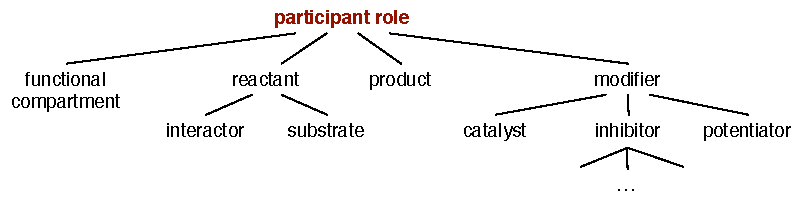
\includegraphics[scale = 0.87]{figs/sbo-participant-role}
  \caption{Partial expansion of some of the terms in the
    \emph{participant role} branch of SBO.}
  \label{fig:expanded-speciesRef}
\end{figure}

The controlled vocabulary for quantitative parameters is
illustrated in \fig{fig:expanded-parameter}.  Note the
separation of \emph{kinetic constant} into separate terms for
unimolecular, bimolecular, etc. reactions, as well as for forward
and reverse reactions.  The need to have separate terms for
forward and reverse rate constants arises in reversible
mass-action reactions.  This distinction is not always necessary
for all quantitative parameters; for example, there is no
comparable concept for the Michaelis constant.  Another
distinction for some quantitative parameters is decomposition into
different versions based on the modeling framework being assumed.
For example, different terms for continuous and discrete
formulations of kinetic constants represent specializations of the
constants for particular simulation frameworks.  Not all
quantitative parameters will need to be distinguished along this
dimension.

\begin{figure}[tbh]
  \centering
  \vspace{-2ex}
  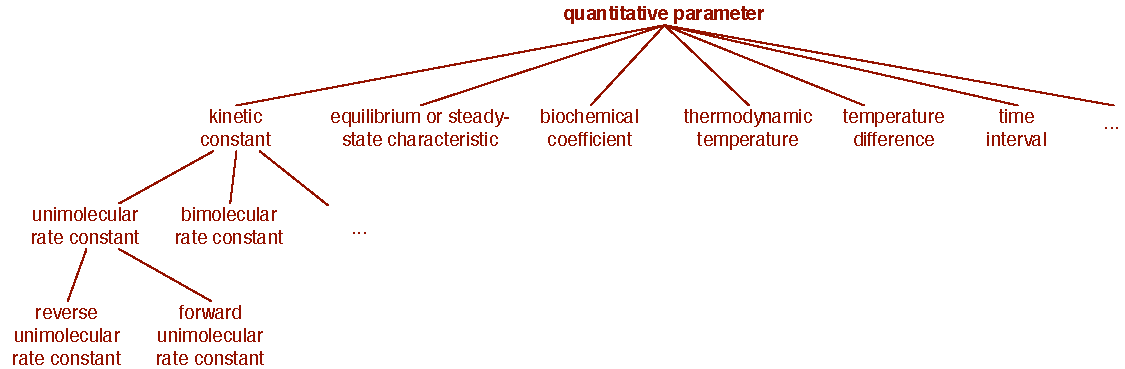
\includegraphics[scale = 0.86]{figs/sbo-quantitative-parameter}
  \caption{Partial expansion of some of the terms in the
    \emph{quantitative parameter} branch.}
  \label{fig:expanded-parameter}
\end{figure}

The terms of the SBO quantitative \changed{systems description} parameter branch contain
mathematical formulas that are encoded using \mathmltwo; these
formulas define the parameter value using other SBO parameters.
The main use of this approach is to avoid listing all the variants
of a mathematical expression, escaping a combinatorial explosion.

The \emph{modeling framework} controlled vocabulary is needed to
elucidate how to simulate a mathematical expression used in models.
\fig{fig:expanded-framework} illustrates the structure of
this branch, which is at this point \changed{fairly}  simple, but we
expect that more terms will evolve in the future.

\begin{figure}[tbh]
  \centering
  \vspace{-1ex}
  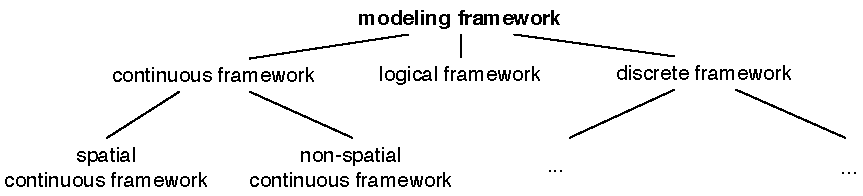
\includegraphics[scale = 0.83]{figs/sbo-framework}
  \caption{Partial expansion of some of the terms in the
    \emph{modeling framework} branch.}
  \label{fig:expanded-framework}
\end{figure}

The \emph{mathematical expression} vocabulary encompasses the
various mathematical expressions that constitute a model.
\fig{fig:sbo-math-expression} illustrates a portion of the
hierarchy.  Rate law or conservation law formulas are part of the
mathematical expression hierarchy, and subdivided by successively
more refined distinctions until the leaf terms represent precise
statements of common reaction or rule types.  Other types of
mathematical expressions may be included in the future in order to
be able to further characterize mathematical components of a
model, such as initial assignments, assignment rules, rate rules,
algebraic rules, constraints, and event triggers and assignments.

\begin{figure}[tbh]
  \centering
  \vspace*{-1ex}
  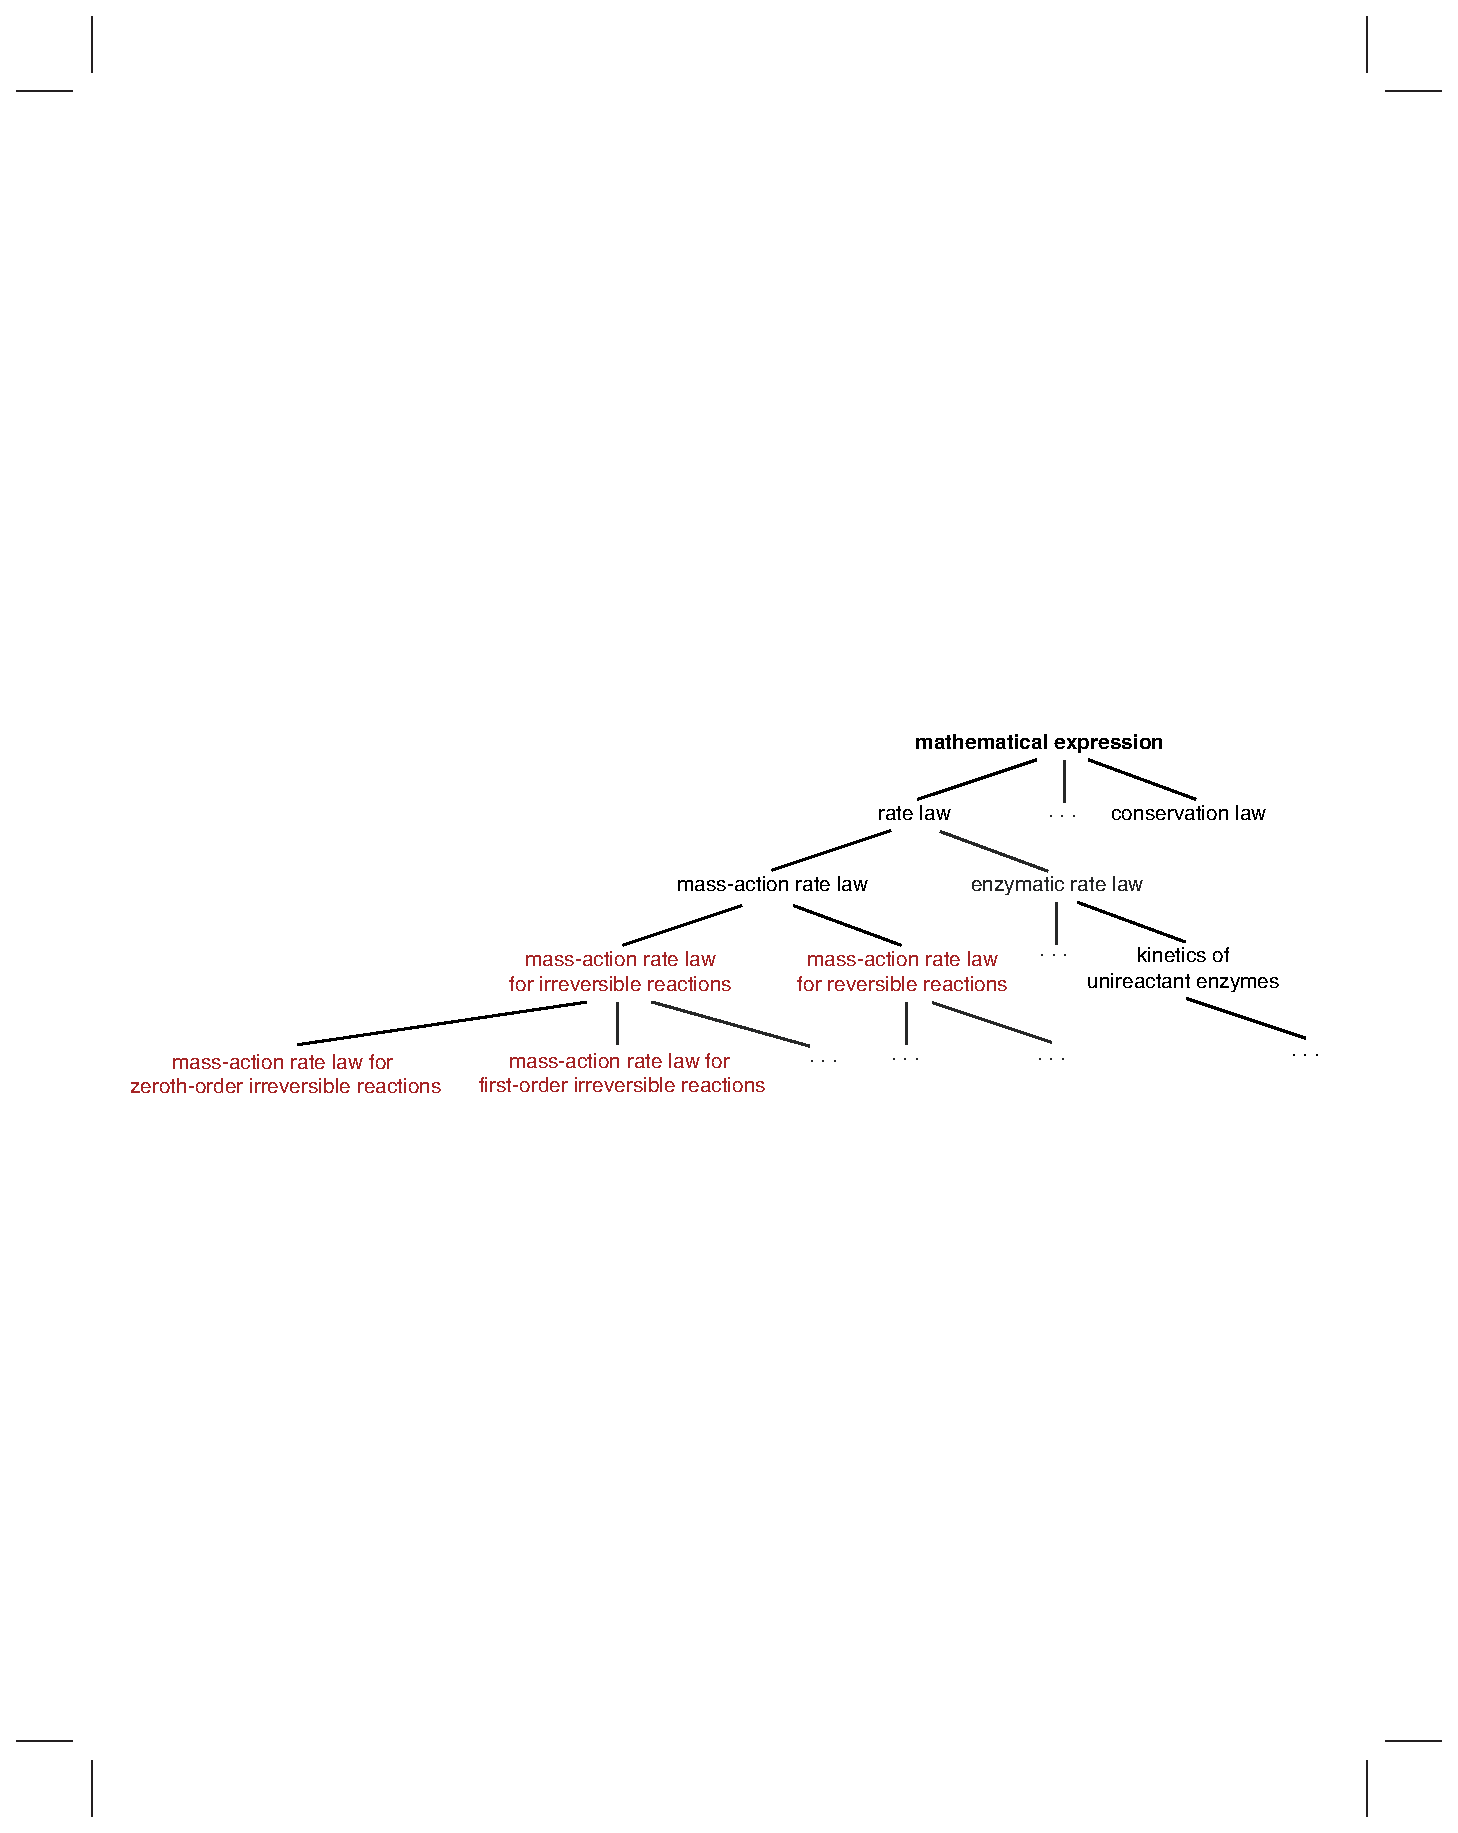
\includegraphics[scale = 0.8, trim=10 0 0 0]{figs/sbo-math-expression}
  \caption{Partial expansion of some of the terms in the \emph{mathematical
      expression} branch.}
  \label{fig:sbo-math-expression}
\end{figure}

The leaf terms of the mathematical expression branch contain the
mathematical formulas encoded using \mathmltwo.  There are many
potential uses for this.  One is to allow a software application
to obtain the formula corresponding to a term and use it as the
basis of an expression to insert into a model.  In effect, the
formulas given in the CV act as templates for what to put into an
SBML construct such as \KineticLaw or \Rule.  The MathML
definition also acts as a precise statement about the rate law in
question. In particular, it carries information about the modeling
framework to use in order to interpret the formula.  Some of the
non-leaf terms also contain formulas encoded using \mathmltwo. In
that case, the formulas contained in the children terms are
specific versions of the formula contained in the parent term.
Those formulas may be generic, containing MathML constructs not
yet supported by SBML, and need to be expanded into the MathML
subset allowed in SBML before they can be used in conjunction with
SBML models.

To make this discussion concrete, here is an example definition of
an entry in the SBO rate law hierarchy at the time of this
writing.  This term represents second-order, irreversible,
mass-action rate laws with one reactant, formulated for use in a
continuous modeling framework:
\begin{description}

\item \emph{ID}: \token{SBO:0000052}

\item \emph{Name}: mass-action rate law for second-order
  irreversible reactions, one reactant, continuous scheme

\item \emph{Definition}: Reaction scheme where the products are
  created from the reactants and the change of a product quantity
  is proportional to the product of reactant activities. The
  reaction scheme does not include any reverse process that
  creates the reactants from the products. The change of a product
  quantity is proportional to the square of one reactant quantity.
  It is to be used in a reaction modeled using a continuous
  framework.

\item \emph{Parent(s)}: \\
  \token{SBO:0000050}: mass-action rate law for second-order
    irreversible reactions, one reactant (\emph{is-a}).
    \\
    \token{SBO:0000163}: mass-action rate law for irreversible
    reactions, continuous sceheme (\emph{is-a}).
  
\item \emph{MathML}:\vspace*{-1ex}
  \begin{example}
<math xmlns="http://www.w3.org/1998/Math/MathML">
   <semantics definitionURL="http://biomodels.net/sbo/#SBO:0000062">
      <lambda>
         <bvar><ci definitionURL="http://biomodels.net/sbo/#SBO:0000036">k</ci></bvar>
         <bvar><ci definitionURL="http://biomodels.net/sbo/#SBO:0000509">R</ci></bvar>
         <apply>
            <times/>
            <ci>k</ci>
            <ci>R</ci>
            <ci>R</ci>
         </apply>
      </lambda>
   </semantics>
</math>
\end{example}

\end{description}

In the MathML definition of the term shown above, the bound
variables in the \token{lambda} expression are tagged with
references to terms in the SBO \emph{\changed{systems description} parameter} \changed{branch} (for
\token{k} \changed{and} \token{R}).  This makes it
possible for software applications to interpret the intended
meanings of the parameters in the expression.  This also permits
to convert an expression into another, by using the \mathmltwo
formula contained in the SBO terms associated with the parameters.

The \emph{\changed{occurring entity representation}} branch of SBO defines types of biological
processes, events or relationship involving entities.  It lists
the types of biochemical reactions, such as binding,
conformational transition, or cleavage, and also the different
controls that modify a biochemical reaction, such as inhibition,
catalysis, etc.

\begin{figure}[tbh]
  \centering
  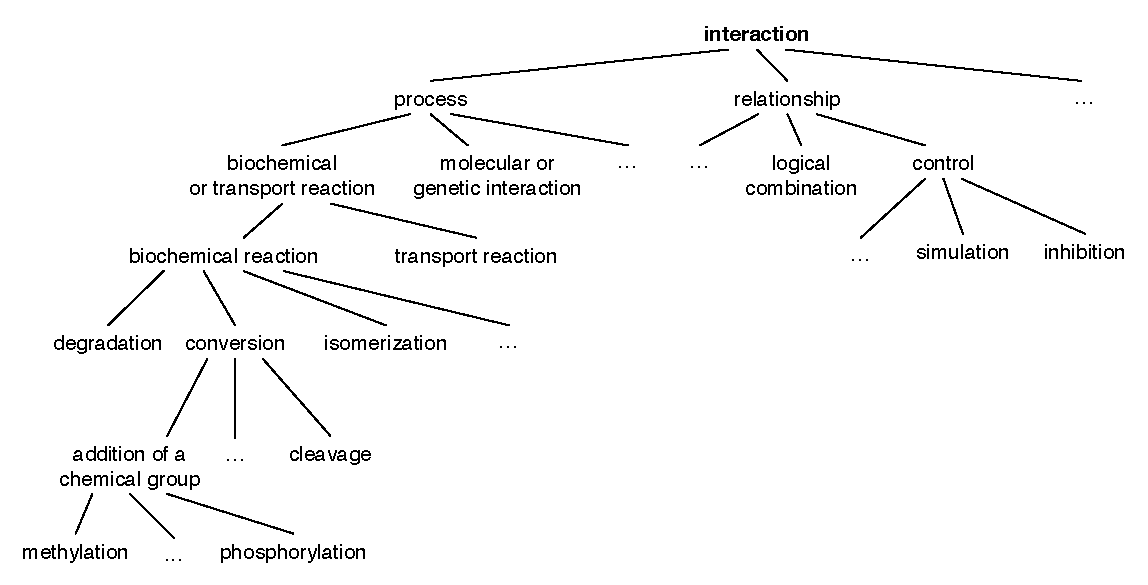
\includegraphics[scale = 0.82]{figs/sbo-interaction}
  \caption{Partial expansion of some of the terms in the \emph{\changed{occurring entity representation}} branch.}
  \label{fig:sbo-interaction}
\end{figure}

One of the goals of SBO is to permit a tool to traverse up and
down the hierarchy in order to find equivalent terms in different
frameworks.  The hope is that when a software tool encounters a
given rate formula in a model, the formula will be a specific form
(say, ``mass-action rate law, second order, one reactant, for
discrete simulation''), but by virtue of the consistent
organization of the reaction rate CV into framework-specific
definitions, and the declaration of every parameters involved in
each expression, the tool should in principle be able to determine
the definitions for other frameworks (say, ``mass-action rate law,
second order, one reactant for \emph{continuous} simulation'').
If the software tool is designed for continuous simulation and it
encounters an SBML model with rate laws formulated for discrete
simulation, it could in principle look up the rate laws'
identifiers in the CV and search for alternative definitions
intended for discrete simulation.  And of course, the converse is
true, for when a tool designed for discrete simulation encounters
a model with rate laws formulated for continuous simulation.

\begin{figure}[htb]
  \centering
  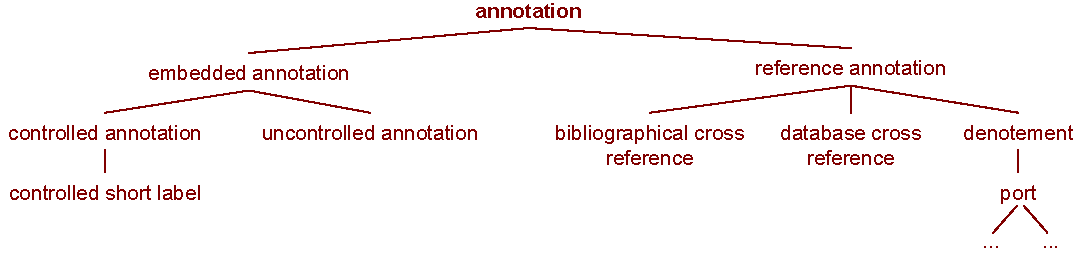
\includegraphics[scale = 0.87]{figs/sbo-annotation}
  \caption{\changed{Current expansion of the terms in the
    \emph{annotation} branch of SBO.}}
  \label{fig:sbo-annotation}
\end{figure}

\begin{blockChanged}
The controlled vocabulary for annotations is illustrated in \fig{fig:sbo-annotation}, the single child of the \emph{metadata representation} branch of SBO.  As this branch is for annotating annotations themselves, its branches cannot usually be used for \SBase-derived objects, as those generally depict basic model information, and not annotations for that model.  However, there are packages which may be able to use this branch of SBO:  the \val{port} element exactly corresponds to the \class{Port} class from the SBML Level~3 Hierarchical Model Composition package, for example.

% Lucian:  I was hoping that adding this paragraph would push Table 6 down some so it didn't look goofy, but no luck.  Left it here in case we want to put it in anyway.
%
%As SBO and SBML develop further, new branches may be added to SBO that correspond to new packages for SBML.  When possible, that package specification will describe those new relationships, although it will always be legal to use the new terms in advance of the specifications being updated.
\end{blockChanged}


\subsubsection{Tradeoffs in using SBO terms}

The SBO-based approach to annotating SBML components with
controlled terms has the following strengths:
\begin{enumerate}

\item The syntax is minimally intrusive and maximally simple,
  requiring only one string-valued attribute.

\item It supports a significant fraction of what SBML users have wanted
  to do with controlled vocabularies.

\item It does not interfere with any other scheme.  The more
  general annotation-based approach described in
  \sec{sec:annotation-standard} can still be used
  simultaneously in the same model.

\end{enumerate}

The scheme has the following weaknesses:
\begin{enumerate}

\item An object can only have one \token{sboTerm} attribute;
  therefore, it can only be related to a single term in SBO.
  (This also impacts the design of SBO: it must be structured such
  that a class of SBML elements can logically only be associated
  with one class of terms in the ontology.)

\item The only relationship that can be expressed by
  \token{sboTerm} is ``is a''.  It is not possible to represent
  different relationships (known as \emph{verbs} in
  ontology-speak).  This limits what can be expressed using SBO.

\end{enumerate}



The weaknesses are not shared by the annotation scheme described
in \sec{sec:annotation-standard}.  


\subsubsection{Relationships between individual SBML components and SBO terms}

The \token{sboTerm} attribute is defined on the abstract class
\SBase and can be used in all derived elements.  However, not all
SBO terms should be used to annotate all SBML elements.
\tab{tab:sboterm-availability} summarizes the relationships
between SBML components and the branches within SBO that apply to
that component. (There are currently no specific SBO term that
correspond to the \SBML, \UnitDefinition, \Unit, and various
\class{ListOf\rule{0.5in}{0.5pt}} list classes.)

\begin{table}[ht]
  \small
  \centering
  \begin{tabular}{lll}
    \toprule
    \textbf{SBML Component} & \textbf{SBO Branch} & \textbf{Branch Identifier} \\
    \midrule
    \Model              & \changed{occurring entity representation}			& \sbointeractionID \\
    \FunctionDefinition & mathematical expression   	& \sbomathformulaID \\
    \Compartment        & material entity 		& \sbomaterialentityID \\
    \Species            & material entity 		& \sbomaterialentityID \\
    \Reaction           & \changed{occurring entity representation}     		& \sbointeractionID \\
    \Parameter          & quantitative \changed{systems description} parameter    	& \sboparameterID \\
    \SpeciesReference   & participant role          	& \sboparticipantroleID \\
    \ModifierSpeciesReference & participant role	& \sboparticipantroleID \\
    \KineticLaw         & rate law                  	& \sboratelawID \\
    \LocalParameter     & quantitative \changed{systems description} parameter    	& \sboparameterID \\
    \InitialAssignment  & mathematical expression   	& \sbomathformulaID \\
    \AlgebraicRule      & mathematical expression   	& \sbomathformulaID \\
    \AssignmentRule     & mathematical expression   	& \sbomathformulaID \\
    \RateRule           & mathematical expression   	& \sbomathformulaID \\
    \Constraint         & mathematical expression   	& \sbomathformulaID \\
    \Event              & \changed{occurring entity representation}     		& \sbointeractionID \\
    \Trigger            & mathematical expression   	& \sbomathformulaID \\
    \Priority           & mathematical expression   	& \sbomathformulaID \\
    \Delay              & mathematical expression   	& \sbomathformulaID \\
    \EventAssignment    & mathematical expression   	& \sbomathformulaID \\
    \bottomrule
  \end{tabular}
  \caption{SBML components and the main types of SBO terms that
    may be assigned to them.  The identifiers of the highest-level
    SBO terms in each branch are provided for guidance, but actual
    values used for \token{sboTerm} attributes should be more
    specific child terms within these branches.  Note that the
    important aspect here is the set of specific SBO identifiers,
    not the SBO term names, because the names may change as SBO
    continues to evolve. See text for further explanations.} 
  \label{tab:sboterm-availability}
\end{table}

The parent identifiers shown in
\tab{tab:sboterm-availability} are provided for reference.
They are the highest-level terms in their respective branch;
however, these are \emph{not} the terms that would be used to
annotate an element in SBML, because there are more specific terms
underneath the parents shown here.  A software tool should use the
most specific SBO term available for a given concept rather than
using the top-level identifier acting as the root of that
particular vocabulary.


\subsection{Relationships to the SBML \tokenNC{annotation} element}

Another way to provide this information would be to place SBO
terms inside the \SBase \token{annotation} element
(\sec{sec:sbase} and \sec{sec:annotation-standard}).
However, in the interest of making the use of SBO in SBML as
interoperable as possible between software tools, the
best-practice recommendation is to place SBO references in the
\token{sboTerm} attribute rather than inside the
\token{annotation} element of an object. If instead the approach
of using \token{annotation} is taken, the qualifiers
(\sec{sec:qualified-dc-annotation}) linking the SBML
element and SBO term should be chosen extremely carefully, since
it will no longer be possible to assume an ``instance to class''
relationship.

Although \token{sboTerm} is just another kind of optional
annotation in SBML, SBO references are separated into
their own attribute on SBML components, both to simplify their use
for software tools and because doing so asserts a stronger and
more focused connection in a more regimented fashion.  SBO
references are intended to allow a modeler to make a statement of
the form ``this object is identical in meaning and intention to
the object defined in the term X of SBO'', and do so in a way
that a \emph{software tool can interpret unambiguously}.

Some software applications may have their own vocabulary of terms
similar in purpose to SBO.  For maximal software interoperability,
the best-practice recommendation in SBML is nonetheless to use SBO
terms in preference to using application-specific annotation
schemes.  Software applications should therefore attempt to
translate their private terms to and from SBO terms when writing
and reading SBML, respectively.


\subsection{Discussion}

Here we discuss some additional points about the SBO-based
approach.

\subsubsection{Frequency of change in the ontology}
\label{sec:sbo-frequency-of-change}

The SBO development approach follows conventional ontology
development approaches in bioinformatics.  One of the principles
being followed is that identifiers and meanings of terms in the
CVs never change and the terms are never deleted.  Where some
terms are deemed obsolete, the introduction of new terms refine or
supersede existing terms, but the existing identifiers are left in
the CV.  Thus, references never end up pointing to nonexistent
entries.  In the case where synonymous terms are merged after
agreement that multiple terms are identical, the term identifiers
are again left in the CV and they still refer to the same concept
as before.  Out-of-date terms cached or hard-coded by an
application remain usable in all cases.  (Moreover,
machine-readable CV encodings and appropriate software design
should render possible the development of API libraries that
automatically map older terms to newer terms as the CVs evolve.)
Therefore, a model is never in danger of ending up with SBO
identifiers that cannot be dereferenced.  If an application finds
an old model with a term \token{SBO:0000065}, it can be assured
that it will be able to find this term in SBO, even if it has been
superseded by other, more preferred terms.


\subsubsection{Consistency of information}

If you have a means of linking (say) a reaction rate formula to a
term in a CV, it is possible to have an inconsistency between the
formula in the SBML model and the one defined for the CV term.
However, this is not a new problem; it arises in other situations
involving SBML models already.  The guideline for these situations
is that the model must be self-contained and stand on its own.
Therefore, in cases where they differ, the definitions in the SBML
model take precedence over the definitions referenced by the CV.
In other words, the model (and its MathML) is authoritative.


\subsubsection{Implications for network access}
\label{sec:sbo-implications-for-network-access}

A software tool does not need to have the ability to access the
network or read the CV every time it encounters a model or
otherwise works with SBML.  Since the SBO will likely stabilize
and change infrequently once a core set of terms is defined,
applications can cache the controlled vocabulary, and not make
network accesses to the master SBO copy unless something forces
them to (\eg detecting a reference in a model to an SBO term that
the application does not recognize).  Applications could have user
preference settings indicating how often the CV definitions should
be refreshed (similar to how modern applications provide a setting
dictating how often they should check for new versions of
themselves).  Simple applications may go further and hard code
references to terms in SBO that have reached stability and
community consensus. SBO is available for download under different
formats (\sboref).  Web services are also available to provide
programmatic access to the ontology.

% -*- TeX-master: "sbml-level-2-version-4"; fill-column: 66 -*-
% $Id$
% $HeadURL$
% ----------------------------------------------------------------

\section{A standard format for the \token{annotation} element}
\label{sec:finney-novere}
\label{sec:annotation-standard}

This section describes the recommended non-proprietary
format for the content of \token{annotation} elements
in SBML when (a) referring to controlled vocabulary
terms and database identifiers which define and describe
biological and biochemical entities, and (b) describing the
creator of a model and its modification history. Such a structured
format should facilitate the generation of models compliant with
the MIRIAM guidelines for model curation~\citep{le_novere:2005}.

This format should \emph{not} be used to refer to SBO terms
(Section~\ref{sec:sboTerm}), because SBO defines terms about
mathematical modeling constructs and not the biological and
biochemical entities that the mathematics represent.

The format described in this section is intended to be the form of
one of the top-level elements that could reside in an
\token{annotation} element attached to an SBML object derived from
\SBase.  The element is named \token{rdf:RDF}.  The format
described here is compliant with the constraints placed on the
form of annotation elements described in
Section~\ref{sec:annotation-use}.  We refer readers to
Section~\ref{sec:annotation-use} for important information on the
structure and organization of application-specific annotations;
these are not described here.


\subsection{Motivation}

The SBML structures described elsewhere in this document do not
have any biochemical or biological semantics.  The format
described in this section provides a scheme for linking SBML
structures to external resources so that those structures can have
such semantics.  The motivation for the introduction of this
scheme is similar to that given for the introduction of
\token{sboTerm}; however, this scheme is significantly more
flexible.


\subsection{XML namespaces in the standard annotation}

This format uses a restricted form of Dublin
Core~\citep{DCMI:2003} and BioModels qualifier elements (see
\url{http://www.ebi.ac.uk/compneur-srv/miriam-main/mdb?section=qualifiers}) embedded in
RDF~\citep{w3c:2004}. It uses a number of external XML standards
and associated XML namespaces.
Table~\ref{tab:namespaces-for-standard-annotation} lists these
namespaces and relevant documentation on those namespaces.  The
format constrains the order of elements in these namespaces beyond
the constraints defined in the standard definitions for those
namespaces.  For each standard listed, the format only uses a
subset of the possible syntax defined by the given standard.  Thus
it is possible for an \token{annotation} element to include XML
that is compliant with those external standards but is not
compliant with the format described here.  Parsers wishing to
support this format should be aware that a valid
\token{annotation} element may contain an \token{rdf:RDF} element
which is not compliant with the format described here.  A parser
should check that all aspects of the syntax defined here before
assuming that the contained data is encoded in the format.

\begin{table}[bh]
  \vspace*{3ex}
  \small
  \centering
  \begin{edtable}{tabular}{lll}
    \toprule
& Namespace URI & Definition Document \\
    \midrule
    \token{dc} & \uri{http://purl.org/dc/elements/1.1/} & \cite{powell:2003}\\
    \token{rdf} & \uri{http://www.w3.org/1999/02/22-rdf-syntax-ns\#} & \cite{w3c:2004b} \\
    \token{dcterms} & \uri{http://purl.org/dc/terms/} & \cite{kokkelink:2002}\\
    & & \cite{DCMIUB:2005} \\
    \token{vcard} & \uri{http://www.w3.org/2001/vcard-rdf/3.0\#} & \cite{iannella:2001} \\
    \token {bqbiol} & \uri{http://biomodels.net/biology-qualifiers/} \\
    \token {bqmodel} & \uri{http://biomodels.net/model-qualifiers/} \\
    \bottomrule
  \end{edtable}
  \vspace*{-0.95ex}
  \caption{The XML standards used in the SBML standard format for annotation.
  The namespace prefix are shown to indicate only the prefix used in the main text.}
  \label{tab:namespaces-for-standard-annotation}
\end{table}


% The default page break is too awkward here.
\clearpage

%=============================================================================
\subsection{General syntax for the standard annotation}
%=============================================================================

An outline of the format syntax is shown below.

\vspace*{0.1ex}

\begin{example}
<SBML_ELEMENT +++ metaid="SBML_META_ID" +++ >
  +++
  <annotation>
    +++
    <rdf:RDF
      xmlns:rdf="http://www.w3.org/1999/02/22-rdf-syntax-ns\#"
      xmlns:dc="http://purl.org/dc/elements/1.1/"
      xmlns:dcterm="http://purl.org/dc/terms/"
      xmlns:vcard="http://www.w3.org/2001/vcard-rdf/3.0\#"
      xmlns:bqbiol="http://biomodels.net/biology-qualifiers/"
      xmlns:bqmodel="http://biomodels.net/model-qualifiers/"
    >
      <rdf:Description rdf:about="#SBML_META_ID">
        [MODEL_HISTORY]
        <RELATION_ELEMENT>
          <rdf:Bag>
            <rdf:li rdf:resource="URI" />
            ...
          </rdf:Bag>
        </RELATION_ELEMENT>
        ...
      </rdf:Description>
      +++
    </rdf:RDF>
    +++
  </annotation>
  +++
</SBML_ELEMENT>
\end{example}

The above outline shows the order of the elements. The capitalized
identifiers refer to generic strings of a particular type:
\texttt{SBML\_ELEMENT} refers to any SBML element name that can
contain an \token{annotation} element; \texttt{SBML\_META\_ID} is
a XML \primtype{ID} string; \texttt{RELATION\_ELEMENT} refers to
element names in either the namespace
\uri{http://biomodels.net/biology-qualifiers/} or
\uri{http://biomodels.net/model-qualifiers/}; and \texttt{URI} is
a URI.  \texttt{[MODEL\_HISTORY]} refers to an optional section
described in Section~\ref{sec:model-history-annotation} which can
only be present within SBML model elements. `\texttt{+++}' is a
placeholder for either no content or valid XML syntax that is not
defined by the standard annotation scheme but is consistent with
the relevant standards for the enclosing elements. `\texttt{...}'
is a placeholder for zero or more elements of the same form as the
immediately preceding element.  The precise form of whitespace and
the XML namespace prefix definitions is not constrained; however,
the elements and attributes must be in the namespaces shown. The
rest of this section describes the format formally in English.

In this format, the annotation of an element is located in a single
\token{rdf:RDF} element contained within an SBML
\token{annotation} element. The annotation element can contain
other elements in any order as described in 
Section~\ref{sec:annotation-use}.  The format described in this
section only defines the form of the \token{rdf:RDF} element. The
containing SBML \SBase element must have a \token{metaid} attribute
value. (As this attribute is of the type \primtype{ID} its value
must unique to the entire SBML document.)

The first element of the \token{rdf:RDF} element must be an
\token{rdf:Description} element with an \token{rdf:about}
attribute. (This format doesn't define the form of subsequent
elements of the \token{rdf:RDF} element.) The value of the
\token{rdf:about} attribute must be of the form
\texttt{\#<string>} where the string component is equal to the
value of the \token{metaid} attribute of the containing SBML element.

The \token{rdf:Description} element can contain only an optional
model history section (see
Section~\ref{sec:model-history-annotation}) followed by a sequence
of zero or more BioModels relation elements. The optional model
history section can only be present within an SBML \Model element.
The specific type of the relation elements will vary depending on
the relationship between the SBML component and referenced
information or resource.

Although Section~\ref{sec:qualified-dc-annotation} describes the
detailed semantics of each of the relation element types, the
content of these elements follows the same form.  The BioModels
qualifiers relation elements must only contain a single
\token{rdf:Bag} element which in turn must only contain one or
more \token{rdf:li} elements.  The \token{rdf:li} elements must
only have a \token{rdf:resource} attribute containing a URI
referring to an information resource (See
Section~\ref{sec:uri-in-annotation}).

Annotations in this format can be located at different depths
within a model component.

%=============================================================================
\subsection{Use of URIs}
\label{sec:uri-in-annotation}
%=============================================================================

The format represents a set of relationships between the SBML
element and the resources referred to by the contained
\token{rdf:resource} attribute values.  The BioModels relation
elements simply define the type of the relationship.

\begin{blockChanged}

For example, a \Species element representing a protein could be
annotated with a reference to the database UniProt by the
\uri{urn:miriam:uniprot:P12999} resource identifier,
identifying exactly the protein described by the \Species element.
This identifier maps to a unique entry in UniProt which is never
deleted from the database. In the case of UniProt, this is the
``accession'' of the entry. When the entry is merged with another
one, both ``accession'' are conserved. Similarly in a controlled
vocabulary resource, each term is associated with a perennial
identifier. The UniProt entry also possess an ``entry name'' (the
Swiss-Prot ``identifier''), a ``protein name'', ``synonyms'' etc.
Only the ``accession'' is perennial and should be used.

The value of a \token{rdf:resource} attribute is a URI that both
uniquely identifies the resource, and the data in the resource. 
The value of the \token{rdf:resource} attribute is a URI, not a
URL; as such, a URI does not have to reference a physical web
object but simply identifies a controlled vocabulary term or
database object (a URI is a label). For instance, a true URL for an Internet
resource such as \uri{http://www.uniprot.org/entry/P12999} might
correspond to the URI \uri{urn:miriam:uniprot:P12999}.

SBML does not specify how a parser is to interpret a URI. In the
case of a transformation into a physical URL, there could be
several solutions. For example, the URI
\uri{urn:miriam:obo.go:GO\%3A0007268} can be translated
into:

\end{blockChanged}

\noindent \uri{http://www.ebi.ac.uk/ego/DisplayGoTerm?selected=GO:0007268}\\
\noindent \uri{http://www.godatabase.org/cgi-bin/amigo/go.cgi?view=details\&query=GO:0007268}\\
\noindent \uri{http://www.informatics.jax.org/searches/GO.cgi?id=GO:0007268}

\begin{blockChanged}

Similarly the URI \uri{urn:miriam:ec-code:3.5.4.4}
can refer to:
\end{blockChanged}

\noindent \uri{http://www.ebi.ac.uk/intenz/query?cmd=SearchEC\&ec=3.5.4.4}\\
\noindent \uri{http://www.expasy.org/cgi-bin/nicezyme.pl?3.5.4.4}\\
\noindent \uri{http://www.chem.qmul.ac.uk/iubmb/enzyme/EC3/5/4/4.html}\\
\noindent \uri{http://www.genome.jp/dbget-bin/www\_bget?ec:3.5.4.4}\\
\noindent etc.

To enable interoperability, the community has agreed on an initial
set of standardized valid URI syntax rules which may be used
within the standard annotation format. This set of rules is not
part of the SBML standard but will grow independently from
specific SBML Levels and Versions. As the set changes, a given URI
syntax rule will not be modified, although the physical resources
associated with the rule may change. These URIs will always be
composed as \token{resource:id}. The MIRIAM resources
\url{http://www.ebi.ac.uk/compneur-srv/miriam-main/} lists URI syntaxes and
possible physical links to controlled vocabulary and databases.
Each entry contains a list of SBML and relation elements in which
the given URI can be appropriately embedded. To enable consistent
and thus useful links to external resources, the URI syntax rule
set must have a consistent view of the concepts represented by the
different SBML elements for the purposes of this format.  For
example as the rule set is designed to link SBML biological and
biochemical resources the rule set assumes that a \Species element
represents the concept of a biochemical entity type rather than
mathematical symbol. The URI rule list will evolve with the
evolution of databases and resources. The annotation format
described in this section does not require a simple parser of this
format to access this list.


%=============================================================================
\subsection{Relation elements}
\label{sec:qualified-dc-annotation}
%=============================================================================

To enable the format to encode different types of relationships
between SBML elements and resources, different BioModel qualifier
elements are used to enclose a set of \token{rdf:li} elements. The
relation elements imply a specific relationship between the
enclosing SBML element and the resources referenced by the
\token{rdf:li} elements.

The detailed semantics (i.e. from the perspective of automatic
parser) of the relation elements is defined by the URI list at
\url{http://www.ebi.ac.uk/compneur-srv/miriam-main/}, and thus is outside the
scope of SBML. The URI list generally assumes that the biological
entity represented by the element is the concept linked to the
reference resource.

Several relation elements with a given tag, enclosed in the same
SBML element, each represent an alternative annotation to the SBML
element. For example two \token{bqbiol:hasPart} elements within a
\Species SBML element represent two different sets of
references to the parts making up the the chemical entity
represented by the species. (The species is not made up of all the
entities represented by all the references combined).

The complete list of the qualifier elements in the Biomodels
qualifier namespaces is documented at
\url{http://www.ebi.ac.uk/compneur-srv/miriam-main/mdb?section=qualifiers}. The list is
divided into two namespaces one for model qualifiers
\uri{http://biomodels.net/biology-qualifiers/} (prefix used here
\token{bqbiol}) and the other for biological qualifiers
\uri{http://biomodels.net/model-qualifiers/}) (prefix used here
\token{bqmodel}.  This list will only grow i.e no element will be
removed from the list. The following is the list of elements at
the time of writing:

%\begin{figure}[htb]
%  \vspace*{2pt}
%  \centering
%\[
%%\begin{CD}
%\textrm{SBML Element}  @>{qualifier}>> \textrm{Referenced Resource} \\
%@VV{represents}V                @VV{represents}V \\
%\textrm{Biological Entity A}   @>{relationship}>>
%\textrm{Biological Entity B}
%%\end{CD}
%\]
%  \caption{How the relationship between biological
%  entities are defined using relations between resources}
%  \label{fig:lenovere-annotation}
%\end{figure}

\begin{itemize}

\item \token{bqmodel:is} The modeling object encoded by the SBML
  component is the subject of the referenced resource. For
  instance, this qualifier might be used to link the model to a
  model database.

\item \token{bqmodel:isDescribedBy} The modeling object
  encoded by the SBML component is described by
  the referenced resource. This relation might be used to link
  SBML components to the literature that describes this model or
  this kinetic law.

\item \token{bqbiol:is} The biological entity represented by the
  SBML component is the subject of the referenced resource. This
  relation might be used to link a reaction to its exact
  counterpart in (e.g.) KEGG or Reactome.

\item \token{bqbiol:hasPart} The biological entity represented by
  the SBML component includes the subject of the referenced
  resource, either physically or logically. This relation might be
  used to link a complex to the description of its components.

\item \token{bqbiol:isPartOf} The biological entity represented by
  the SBML component is a physical or logical part of the subject
  of the referenced resource. This relation might be used to link
  a component to the description of the complex it belongs to.

\item \token{bqbiol:isVersionOf} The biological entity represented
  by the SBML component is a version or an instance of the subject
  of the referenced resource.

\item \token{bqbiol:hasVersion} The subject of the referenced
  resource is a version or an instance of the biological entity
  represented by the SBML component.

\item \token{bqbiol:isHomologTo} The biological entity represented
  by the SBML component is homolog, to the subject of the
  referenced resource, i.e. they share a common ancestor.

\item \token{bqbiol:isDescribedBy} The biological entity
  represented by the SBML component is described by the referenced
  resource. This relation should be used, for example, to link a
  species or a parameter to the literature that describes the
  quantity of the species or the value of the parameter.

\begin{blockChanged}

\item \token{bqbiol:isEncodedBy} The biological entity represented
  by the model component is encoded, either directly or by virtue
  of transitivity, by the subject of the referenced resource.

\item \token{bqbiol:encodes} The biological entity represented by
  the model component encodes, either directly or by virtue of
  transitivity, the subject of the referenced resource.

\item \token{bqbiol:occursIn}  The biological entity represented by the model component takes place in the subject of the reference resource.

\end{blockChanged}

\end{itemize}

%In all cases using the biology qualifiers, the `object' of the
%relation is the biological or biochemical object represented by
%the enclosing SBML element. In the cases of the model qualifiers,
%the `object' of the relation is the model component encoded by the
%enclosing SBML element. The resources referenced by the
%\class{rdf:li} elements contained within the relation element are
%the `object' of the relation.


%===============================================================
\subsection{Model history}
\label{sec:model-history-annotation}
%================================================================

When enclosed in an SBML \Model element, the format described in
previous sections can include additional elements to describe the
history of the model.  This history data must occur immediately
before the first BioModels relation elements.  These additional
elements encode information on the model creator and a sequence of
dates recording changes to the model. The syntax for this section
is outlined below.

\begin{example}
<dc:creator rdf:parseType="Resource">
  <rdf:Bag>
    <rdf:li rdf:parseType="Resource">
      [[
      +++
      <vCard:N rdf:parseType="Resource">
        <vCard:Family>FAMILY_NAME</vCard:Family>
        <vCard:Given>GIVEN_NAME</vCard:Given>
      </vCard:N>
      +++
      [<vCard:EMAIL>EMAIL_ADDRESS</vCard:EMAIL>]
      +++
      [<vCard:ORG>
        <vCard:Orgname>ORGANIZATION_NAME</vCard:Orgname>
      </vCard:ORG>]
      +++
      ]]
    </rdf:li>
    ...
  </rdf:Bag>
</dc:creator>
<dcterms:created rdf:parseType="Resource">
  <dcterms:W3CDTF>DATE</dcterms:W3CDTF>
</dcterms:created>
{<dcterms:modified rdf:parseType="Resource">
  <dcterms:W3CDTF>DATE</dcterms:W3CDTF>
</dcterms:modified>}
\end{example}

The order of elements is as shown above except that elements of
the format contained between \texttt{[[} and \texttt{]]} can occur
in any order.  The capitalized identifiers refer to generic
strings of a particular type: \texttt{FAMILY\_NAME} is the family
name of a person who created the model; \texttt{GIVEN\_NAME} is
the first name of the same person who created the model;
\texttt{EMAIL\_ADDRESS} is the email address of the same person
who created the model; and \texttt{ORGANIZATION\_NAME} is the name
of the organization with which the same person who created the
model is affiliated \texttt{DATE} is a date in W3C date
format~\citep{wolf:1998}. \texttt{W3CDTF}, \texttt{N},
\texttt{ORG} and \texttt{EMAIL} are literal strings. The elements
of the format contained between \texttt{[} and \texttt{]} are
optional. `\texttt{+++}' is a placeholder for either no content or
valid XML syntax that is not defined by the standard annotation
scheme but is consistent with the relevant standards for the
enclosing elements. `\texttt{...}' is a placeholder for zero or
more elements of the same form as the immediately preceding
element. The precise form of whitespace and the XML namespace
prefix definitions is not constrained.  The remaining text in this
section describes the syntax formally in English.

The additional elements of the model history sub-format consist in
sequence of a \token{dc:creator} element, a
\token{dcterms:created} element and zero or more
\token{dcterms:modified} elements.  All these elements must have
the attribute \token{rdf:parseType} set to \texttt{Resource}.

The \token{dc:creator} element describes the person who created
the SBML encoding of the model and contains a single
\token{rdf:Bag} element.  The \token{rdf:Bag} element can contain
any number of elements; however, the first element must be a
\token{rdf:li} element.  The \token{rdf:li} element can contain
any number of elements in any order.  The set of elements
contained with the \token{rdf:li} element can include the
following informative elements: \token{vCard:N},
\token{vCard:EMAIL} and \token{vCard:ORG}.  The \token{vCard:N}
contains the name of the creator and must consist of a sequence of
two elements: \token{vCard:Family} and the \token{vCard:Given}
whose content is the family (surname) and given (first) names of
the creator respectively.  The \token{vCard:N} must have the
attribute \token{rdf:parseType} set to \texttt{Resource}.  The
content of the \token{vCard:EMAIL} element must be the email
address of the creator.  The content of the \token{vCard:ORG}
element must contain a single \token{vCard:Orgname} element.  The
\token{vCard:Orgname} element must contain the name of an
organization to which the creator is affiliated.

The \token{dcterms:created} and \token{dcterms:modified} elements
must each contain a single \token{dcterms:W3CDTF} element whose
content is a date in W3C date format~\citep{wolf:1998} which is a
a profile of (restricted form of) ISO 8601.


%================================================================
\subsection{Examples}
%=================================================================

The following shows the annotation of a model with model creation
data and links to external resources:

\begin{blockChanged}
\begin{example}
<model metaid="_180340" id="GMO" name="Goldbeter1991_MinMitOscil">
    <annotation>
        <rdf:RDF
                xmlns:rdf="http://www.w3.org/1999/02/22-rdf-syntax-ns\#"
                xmlns:dc="http://purl.org/dc/elements/1.1/"
                xmlns:dcterms="http://purl.org/dc/terms/"
                xmlns:vCard="http://www.w3.org/2001/vcard-rdf/3.0\#"
                xmlns:bqbiol="http://biomodels.net/biology-qualifiers/"
                xmlns:bqmodel="http://biomodels.net/model-qualifiers/"
        >
            <rdf:Description rdf:about="#_180340">
                <dc:creator rdf:parseType="Resource">
                    <rdf:Bag>
                        <rdf:li rdf:parseType="Resource">
                            <vCard:N rdf:parseType="Resource">
                                <vCard:Family>Shapiro</vCard:Family>
                                <vCard:Given>Bruce</vCard:Given>
                            </vCard:N>
                            <vCard:EMAIL>bshapiro@jpl.nasa.gov</vCard:EMAIL>
                            <vCard:ORG>
                                <vCard:Orgname>NASA Jet Propulsion Laboratory</vCard:Orgname>
                            </vCard:ORG>
                        </rdf:li>
                    </rdf:Bag>
                </dc:creator>
                <dcterms:created rdf:parseType="Resource">
                    <dcterms:W3CDTF>2005-02-06T23:39:40+00:00</dcterms:W3CDTF>
                </dcterms:created>
                <dcterms:modified rdf:parseType="Resource">
                    <dcterms:W3CDTF>2005-09-13T13:24:56+00:00</dcterms:W3CDTF>
                </dcterms:modified>
                <bqmodel:is>
                    <rdf:Bag>
                        <rdf:li rdf:resource="urn:miriam:biomodels.db:BIOMD0000000003"/>
                    </rdf:Bag>
                </bqmodel:is>
                <bqmodel:isDescribedBy>
                     <rdf:Bag>
                         <rdf:li rdf:resource="urn:miriam:pubmed:1833774"/>
                     </rdf:Bag>
                </bqmodel:isDescribedBy>
                <bqbiol:isVersionOf>
                    <rdf:Bag>
                        <rdf:li rdf:resource="urn:miriam:kegg.pathway:hsa04110"/>
                        <rdf:li rdf:resource="urn:miriam:reactome:REACT_152"/>
                    </rdf:Bag>
                </bqbiol:isVersionOf>
        </rdf:Description>
    </rdf:RDF>
</annotation>
\end{example}
\end{blockChanged}

The following example shows a \Reaction structure annotated
with a reference to its exact Reactome counterpart.

\begin{blockChanged}
\begin{example}
<reaction id="cdc2Phospho" metaid="jb007">
  <annotation>
    <rdf:RDF
      xmlns:bqbiol="http://biomodels.net/biology-qualifiers/"
      xmlns:rdf="http://www.w3.org/1999/02/22-rdf-syntax-ns\#"
    >
      <rdf:Description rdf:about="#jb007">
        <bqbiol:is>
          <rdf:Bag>
            <rdf:li rdf:resource="urn:miriam:reactome:REACT_6327"/>
          </rdf:Bag>
        </bqbiol:is>
      </rdf:Description>
    </rdf:RDF>
  </annotation>
  <listOfReactants>
    <speciesReference species="cdc2"/>
  </listOfReactants>
  <listOfProducts>
    <speciesReference species="cdc2-Y15P"/>
  </listOfProducts>
  <listOfModifiers>
    <modifierSpeciesReference species="wee1"/>
  </listOfModifiers>
</reaction>
\end{example}
\end{blockChanged}

The following example describes a species that represents a
complex between the protein calmodulin and calcium ions:

\begin{blockChanged}
\begin{example}
<species id="Ca_calmodulin" metaid="cacam">
  <annotation>
    <rdf:RDF
      xmlns:rdf="http://www.w3.org/1999/02/22-rdf-syntax-ns\#"
      xmlns:bqbiol="http://biomodels.net/biology-qualifiers/"
    >
      <rdf:Description rdf:about="\#cacam">
        <bqbiol:hasPart>
          <rdf:Bag>
            <rdf:li rdf:resource="urn:miriam:uniprot:P62158"/>
            <rdf:li rdf:resource="urn:miriam:kegg.compound:C00076"/>
          </rdf:Bag>
        </bqbiol:hasPart>
      </rdf:Description>
    </rdf:RDF>
  </annotation>
</species>
\end{example}
\end{blockChanged}

The following example describes a species that represents either
``Calcium/calmodulin-dependent protein kinase type II alpha
chain'' or ``Calcium/calmodulin-dependent protein kinase type II
beta chain''. This is the case, for example, in the somatic
cytoplasm of striatal medium-size spiny neurons, where both are
present but they cannot be functionally differentiated.

\begin{blockChanged}
\begin{example}
<species id="calcium_calmodulin" metaid="cacam">
  <annotation>
    <rdf:RDF
      xmlns:rdf="http://www.w3.org/1999/02/22-rdf-syntax-ns\#"
      xmlns:bqbiol="http://biomodels.net/biology-qualifiers/"
    >
      <rdf:Description rdf:about="\#cacam">
        <bqbiol:hasVersion>
          <rdf:Bag>
            <rdf:li rdf:resource="urn:miriam:uniprot:Q9UQM7"/>
            <rdf:li rdf:resource="urn:miriam:uniprot:Q13554"/>
          </rdf:Bag>
        </bqbiol:hasVersion>
      </rdf:Description>
    </rdf:RDF>
  </annotation>
</species>
\end{example}
\end{blockChanged}

The above approach should not be used to describe ``any
Calcium/calmodulin-dependent protein kinase type II chain'',
because such an annotation requires referencing the products of
other genes such as gamma or delta. All the known proteins could
be enumerated, but such an approach would almost surely lead to
inaccuracies because biological knowledge continues to evolve.
Instead, the annotation should refer to generic information such
as Ensembl family ENSF00000000194 ``CALCIUM/CALMODULIN DEPENDENT
KINASE TYPE II CHAIN'' or PIR superfamily PIRSF000594
``Calcium/calmodulin-dependent protein kinase type~II''.

%While with \texttt{HasVersion}, the described component could
%represent several alternative, with \texttt{isVersionOf} the
%described component is one of the alternative understated by the
%referenced resource.

The following two examples show how to use the qualifier
\token{isVersionOf}. The first example is the relationship
between a reaction and an EC code. An EC code describes an
enzymatic activity and an enzymatic reaction involving a
particular enzyme can be seen as an instance of this activity. For
example, the following reaction represents the phosphorylation of
a glutamate receptor by a complex calcium/calmodulin kinase II.

\begin{blockChanged}
\begin{example}
<reaction id="NMDAR_phosphorylation" metaid="thx1138">
  <annotation>
    <rdf:RDF
      xmlns:bqbiol="http://biomodels.net/biology-qualifiers/"
      xmlns:rdf="http://www.w3.org/1999/02/22-rdf-syntax-ns\#"
    >
      <rdf:Description rdf:about="#thx1138">
        <bqbiol:isVersionOf>
          <rdf:Bag>
            <rdf:li rdf:resource="urn:miriam:ec-code:2.7.1.17"/>
          </rdf:Bag>
        </bqbiol:isVersionOf>
      </rdf:Description>
    </rdf:RDF>
  </annotation>
  <listOfReactants>
    <speciesReference species="NMDAR"/>
  </listOfReactants>
  <listOfProducts>
    <speciesReference species="P-NMDAR"/>
  </listOfProducts>
  <listOfModifiers>
    <modifierSpeciesReference species="CaMKII"/>
  </listOfModifiers>
  <kineticLaw>
    <math xmlns="http://www.w3.org/1998/Math/MathML">
      <apply>
        <times/>
        <ci>CaMKII</ci>
        <ci>kcat</ci>
        <apply>
          <divide/>
          <ci>NMDAR</ci>
          <apply>
            </times>
            <ci>NMDAR</ci>
            <ci>Km</ci>
          </apply>
        </apply>
      </apply>
    </math>
    <listOfParameters>
      <parameter id="kcat" value="1"/>
      <parameter id="Km" value="5e-10"/>
    </listOfParameters>
  </kineticLaw>
</reaction>
\end{example}
\end{blockChanged}

The second example of the use of \token{isVersionOf} is the
complex between Calcium/calmodulin-dependent protein kinase type
II alpha chain and Calcium/calmodulin, that is only one of the
``calcium- and calmodulin-dependent protein kinase complexes''
described by the Gene Ontology term GO:0005954.

\begin{blockChanged}
\begin{example}
<species id="CaCaMKII" metaid="C8H10N4O2">
  <annotation>
    <rdf:RDF
      xmlns:rdf="http://www.w3.org/1999/02/22-rdf-syntax-ns\#"
      xmlns:bqbiol="http://biomodels.net/biology-qualifiers/"
    >
      <rdf:Description rdf:about="\#C8H10N4O2">
        <bqbiol:isVersionOf>
          <rdf:Bag>
            <rdf:li rdf:resource="urn:miriam:obo.go:GO\%3A0005954"/>
          </rdf:Bag>
        </bqbiol:isVersionOf>
      </rdf:Description>
    </rdf:RDF>
  </annotation>
</species>
\end{example}
\end{blockChanged}

The previous case is different form the following one, although they
could seem similar at first sight. The
``Calcium/calmodulin-dependent protein kinase type II alpha
chain'' is a part of the above mentioned ``calcium- and
calmodulin-dependent protein kinase complex''.

\begin{blockChanged}
\begin{example}
<species id="CaMKIIalpha" metaid="C10H14N2">
  <annotation>
    <rdf:RDF
      xmlns:rdf="http://www.w3.org/1999/02/22-rdf-syntax-ns\#"
      xmlns:bqbiol="http://biomodels.net/biology-qualifiers/"
    >
      <rdf:Description rdf:about="\#C10H14N2">
        <bqbiol:isPartOf>
          <rdf:Bag>
            <rdf:li rdf:resource="urn:miriam:obo.go:GO\%3A0005954"/>
          </rdf:Bag>
        </bqbiol:isPartOf>
      </rdf:Description>
    </rdf:RDF>
  </annotation>
</species>
\end{example}
\end{blockChanged}

It is possible describe a component with several alternative sets
of qualified annotations. For example, the following species
represents a pool of  GMP, GDP and GTP. We annotate it with the
three corresponding KEGG compound identifiers but also with the
three corresponding ChEBI identifiers.  The two alternative
annotations are encoded in separate \token{hasVersion} qualifier
elements.

\begin{blockChanged}
\begin{example}
<species id="GXP" metaid="GXP">
  <annotation>
    <rdf:RDF
      xmlns:rdf="http://www.w3.org/1999/02/22-rdf-syntax-ns\#"
      xmlns:bqbiol="http://biomodels.net/biology-qualifiers/"
    >
      <rdf:Description rdf:about="\#GXP">
        <bqbiol:hasVersion>
          <rdf:Bag>
            <rdf:li rdf:resource="urn:miriam:obo.chebi:CHEBI\%3A17345"/>
            <rdf:li rdf:resource="urn:miriam:obo.chebi:CHEBI\%3A17552"/>
            <rdf:li rdf:resource="urn:miriam:obo.chebi:CHEBI\%3A17627"/>
          </rdf:Bag>
        </bqbiol:hasVersion>
        <bqbiol:hasVersion>
          <rdf:Bag>
            <rdf:li rdf:resource="urn:miriam:kegg.compound:C00035"/>
            <rdf:li rdf:resource="urn:miriam:kegg.compound:C00044"/>
            <rdf:li rdf:resource="urn:miriam:kegg.compound:C00144"/>
          </rdf:Bag>
        </bqbiol:hasVersion>
      </rdf:Description>
    </rdf:RDF>
  </annotation>
</species>
\end{example}
\end{blockChanged}

The following example presents a reaction being actually the
combination of three different elementary molecular reactions. We
annotate it with the three corresponding KEGG reactions, but also
with the three corresponding enzymatic activities.  Again the two
\token{hasPart} elements represent two alternative annotations.
The process represented by the \Reaction structure is
composed of three parts, and  not six parts.

\begin{blockChanged}
\begin{example}
<reaction id="adenineProd" metaid="adeprod">
  <annotation>
    <rdf:RDF
      xmlns:bqbiol="http://biomodels.net/biology-qualifiers/"
      xmlns:rdf="http://www.w3.org/1999/02/22-rdf-syntax-ns\#"
    >
      <rdf:Description rdf:about="\#adeprod">
        <bqbiol:hasPart>
          <rdf:Bag>
            <rdf:li rdf:resource="urn:miriam:ec-code:2.5.1.22"/>
            <rdf:li rdf:resource="urn:miriam:ec-code:3.2.2.16"/>
            <rdf:li rdf:resource="urn:miriam:ec-code:4.1.1.50"/>
          </rdf:Bag>
        </bqbiol:hasPart>
        <bqbiol:hasPart>
          <rdf:Bag>
            <rdf:li rdf:resource="urn:miriam:kegg.reaction:R00178"/>
            <rdf:li rdf:resource="urn:miriam:kegg.reaction:R01401"/>
            <rdf:li rdf:resource="urn:miriam:kegg.reaction:R02869"/>
          </rdf:Bag>
        </bqbiol:hasPart>
      </rdf:Description>
    </rdf:RDF>
  </annotation>
</reaction>
\end{example}
\end{blockChanged}

It is possible to mix different URIs in a given set. The
following example presents two alternative annotations of the human
hemoglobin, the first with ChEBI heme and the second with KEGG
heme.

\begin{blockChanged}
\begin{example}
<species id="heme" metaid="heme">
  <annotation>
    <rdf:RDF
      xmlns:rdf="http://www.w3.org/1999/02/22-rdf-syntax-ns\#"
      xmlns:bqbiol="http://biomodels.net/biology-qualifiers/"
    >
     <rdf:Description rdf:about="\#heme">
       <bqbiol:hasPart>
         <rdf:Bag>
           <rdf:li rdf:resource="urn:miriam:uniprot:P69905"/>
           <rdf:li rdf:resource="urn:miriam:uniprot:P68871"/>
           <rdf:li rdf:resource="urn:miriam:obo.chebi:CHEBI\%3A17627">
         </rdf:Bag>
       </bqbiol:hasPart>
       <bqbiol:hasPart>
         <rdf:Bag>
          <rdf:li rdf:resource="urn:miriam:uniprot:P69905"/>
           <rdf:li rdf:resource="urn:miriam:uniprot:P68871"/>
           <rdf:li rdf:resource="urn:miriam:kegg.compound:C00032"/>
         </rdf:Bag>
       </bqbiol:hasPart>
     </rdf:Description>
   </rdf:RDF>
  </annotation>
</species>
\end{example}
\end{blockChanged}

As formally defined above it is possible to use different
qualifiers in the same annotation element. The following
phosphorylation is annotated by its exact KEGG counterpart and by
the generic GO term ``phosphorylation''.

\begin{blockChanged}
\begin{example}
<reaction id="phosphorylation" metaid="phosphorylation">
  <annotation>
    <rdf:RDF
      xmlns:bqbiol="http://biomodels.net/biology-qualifiers/"
      xmlns:rdf="http://www.w3.org/1999/02/22-rdf-syntax-ns\#"
    >
      <rdf:Description rdf:about="\#phosphorylation">
        <bqbiol:is>
          <rdf:Bag>
            <rdf:li rdf:resource="urn:miriam:kegg.reaction:R03313" />
          </rdf:Bag>
        </bqbiol:is>
        <bqbiol:isVersionOf>
          <rdf:Bag>
            <rdf:li rdf:resource="urn:miriam:obo.go:GO\%3A0016310" />
          </rdf:Bag>
        </bqbiol:isVersionOf>
      </rdf:Description>
    </rdf:RDF>
  </annotation>
</reaction>
\end{example}
\end{blockChanged}

% -*- TeX-master: "sbml-level-3-version-2-core"; fill-column: 66 -*-
% $Id: examples.tex 12140 2010-10-06 05:00:16Z mhucka $
% $HeadURL: https://svn.code.sourceforge.net/p/sbml/code/trunk/specifications/sbml-level-3/version-1/core/spec/examples.tex $
% ----------------------------------------------------------------

% Macros used in this section to provide common typesetting styles.

\newcommand{\species}[1]{\ensuremath{#1}\xspace}
\newcommand{\concent}[1]{\ensuremath{[#1\mkern1mu]}\xspace}
\newcommand{\unit}[1]   {\text{#1}\xspace}

\newcommand{\graybox}[1]{\colorbox[gray]{.85}{#1}}


\section{Example models expressed in XML using SBML}
\label{sec:xml-rep}
\label{sec:examples}

In this section, we present several examples of complete models
encoded in XML using SBML Level~3.


%-----------------------------------------------------------------------------
\subsection{A simple example application of SBML}
\label{sec:modeleg}
%-----------------------------------------------------------------------------

\newcommand{\kon} {\ensuremath{k_\text{on}}\xspace}
\newcommand{\koff}{\ensuremath{k_\text{off}}\xspace}
\newcommand{\kcat}{\ensuremath{k_\text{cat}}\xspace}

Consider the following representation of an enzymatic reaction:
\begin{center}
  \ce{\species{E} + \species{S} <=>[\kon][\koff] \species{ES} ->[\kcat] \species{E} + \species{P}}
\end{center}
In our model, we use the following initial species amounts:
\begin{larray*}
  \species{E}  &=& 5 \cdot 10^{-21} \; \unit{mole} \\
  \species{S}  &=& 10^{-20} \; \unit{mole} \\
  \species{P}  &=& 0 \; \unit{mole} \\ 
  \species{ES} &=& 0 \; \unit{mole}
\end{larray*}
Note that the species quantities are initialized in terms of
substance amounts rather than concentrations.  We also define the
following values for the kinetic constants:
\begin{larray*}
  \kon  &=& 1\:000\:000 \; \unit{litre} \; \unit{mole}^{\,-1} \; \unit{second}^{\,-1}\\
  \koff &=& 0.2 \; \unit{second}^{\,-1}\\
  \kcat &=& 0.1 \; \unit{second}^{\,-1}
\end{larray*}
We place everything in a single compartment we call ``comp'' whose
volume is $10^{-14}$ litres.  The following is a minimal but
complete SBML document encoding this model:

\sbmlexample{enzymekinetics.xml}

The model features local parameter definitions in each reaction.
In this case, the three parameters (\token{kon}, \token{koff},
\token{kcat}) all have unique identifiers and they could also have
just as easily been declared global parameters.  Local parameters
frequently become more useful in larger models, where it may
become tedious to assign unique identifiers for all the different
parameters.

The example above also demonstrates the use of unit specifications
throughout the model.  The \token{model} components define the
units of kinetic laws as being \unit{mole}/\unit{second} by virtue
of the values of the attributes \token{extentUnits} and
\token{timeUnits}.  In the rest of the model, species, parameters
and compartments are defined with appropriate units so that the
mathematical formulas inside the \token{kineticLaw} elements work
out to be \unit{mole}/\unit{second}.


%-----------------------------------------------------------------------------
\subsection{A simple example using the \token{conversionFactor} attribute}
\label{sec:eg:conversionfactor}
%-----------------------------------------------------------------------------

This example involves the same enzymatic reaction as in the
example of Section~\ref{sec:modeleg}:
\begin{center}
  \ce{\species{E} + \species{S} <=>[\kon][\koff] \species{ES} ->[\kcat] \species{E} + \species{P}}
\end{center}
In this new version of the model, we deliberately define the
species with different units from the unit of reaction extent in
the model.  This leads to two illustrative problems: (1) the
reaction rate expressions must be changed in order to reconcile
the differences between the species units and the unit of reaction
extent in the model, and (2) the formulas constructed for species'
rate-of-change equations must use conversion factors to reconcile
the differences between the units of the reaction rate expressions
and the units in which the species quantities are measured.

We begin with the following new \Species object definitions:
\begin{larray*}
  \species{E}   &=& 5 \cdot 10^{-18}\; \unit{millimole} \\
  \species{S}   &=& 10^{-17}\; \unit{millimole} \\
  \species{P}   &=& 0\; \unit{gram} \\
  \species{ES}  &=& 0\; \unit{millimole}
\end{larray*}
We keep the units of extent and time in the model the same as in
Example~\ref{sec:modeleg}; that is, the overall unit of extent in
the model is \unit{mole} and the unit of time is \unit{second},
set by assigning appropriate values to the attributes
\token{extentUnits} and \token{timeUnits}, respectively, on the
\Model object definition.  The differences between these and the
units of the species means that we have to adjust the reaction
rate expressions from their original versions in the model.  In
what follows, we illustrate one approach to doing so, and in
Section~\ref{sec:eg:conversionfactor2} we illustrate a second
approach.  The method in the present section involves changing the
values of the kinetic rate constants in the reaction rate
formulas, while the example of
Section~\ref{sec:eg:conversionfactor2} does not change the kinetic
constants but does require the introduction of additional
parameters.

\newcommand{\veq}    {\ensuremath{v_\text{veq}}\xspace}
\newcommand{\vcat}   {\ensuremath{v_\text{vcat}}\xspace}
\newcommand{\Vcomp}  {\ensuremath{V_\text{comp}}\xspace}
\newcommand{\convE}  {\ensuremath{c_\species{E}}\xspace}
\newcommand{\convS}  {\ensuremath{c_\species{S}}\xspace}
\newcommand{\convP}  {\ensuremath{c_\species{P}}\xspace}
\newcommand{\convES} {\ensuremath{c_{\species{ES}}}\xspace}
\newcommand{\konnew} {\ensuremath{k_\text{on}^{*}}\xspace}
\newcommand{\koffnew}{\ensuremath{k_\text{off}^{*}}\xspace}
\newcommand{\kcatnew}{\ensuremath{k_\text{cat}^{*}}\xspace}

The reaction rate formulas (\ie the formulas in the \token{math}
elements of \KineticLaw objects) were previously
\begin{larray}
  \label{eq:v1}
  \veq  &=& \Vcomp \cdot (\kon \cdot \concent{E} \cdot \concent{S} - \koff \cdot \concent{ES})\\
  \label{eq:v2}
  \vcat &=& \Vcomp \cdot \kcat \cdot \concent{ES}
\end{larray}
where \Vcomp stands for the size of compartment \val{comp} in the
SBML model.  Recalling the values of the parameters \kon, \koff,
and \kcat,
\begin{larray*}
  \kon  &=& 1\:000\:000 \; \unit{litre} \; \unit{mole}^{\,-1} \; \unit{second}^{\,-1}\\
  \koff &=& 0.2 \; \unit{second}^{\,-1}\\
  \kcat &=& 0.1 \; \unit{second}^{\,-1}
\end{larray*}
it becomes clear that, with the values of \species{E}, \species{S}
and \species{ES} all in \unit{millimoles}, Equations~\ref{eq:v1}
and~\ref{eq:v2} no longer lead to units of
\unit{mole}/\unit{second} for the reaction rates.  To compensate,
we change the values of the constants \kon, \koff, and \kcat using
the following simple transformations:
\begin{larray*}
  \konnew = & \kon \cdot \left( \dfrac{1 \; \unit{mole}}{1000 \; \unit{millimoles}} \right)^{2}
  & = 1 \; \unit{litre} \; \unit{mole} \; \unit{millimole}^{-2} \; \unit{second}^{\,-1} \\[4pt]
  \koffnew = & \koff \cdot \dfrac{1 \; \unit{mole}}{1000 \; \unit{millimoles}}
  & = 0.0002 \, \unit{mole} \; \unit{millimole}^{-1} \; \unit{second}^{\,-1} \\[4pt]
  \kcatnew = & \kcat \cdot \dfrac{1 \; \unit{mole}}{1000 \; \unit{millimoles}}
  & = 0.0001 \, \unit{mole} \; \unit{millimole}^{-1} \; \unit{second}^{\,-1}
\end{larray*}\vspace*{0.2ex}
The ``\unit{mole}/\unit{millimole}'' portion of the units are
admittedly unconventional for mass-action kinetic rate constants.
They are unlikely to correspond to values found in textbooks or
databases.  The logic of this approach is that in an actual
experimental situation, with the units of the species as given in
the model (presumably representing how the species are being
measured), the kinetic rate constants are likely to be measured in
terms of the units above.  However, if that is not the case, then
the approach of Section~\ref{sec:eg:conversionfactor2} may be more
appropriate.

\newcommand{\nS}{\ensuremath{n_{\mkern-1muS}}\xspace}
\newcommand{\nP}{\ensuremath{n_{\mkern-1muP}}\xspace}

Taking these new \konnew, \koffnew and \kcatnew parameters and
replacing the original parameters in the reaction rate equations
finally leads to the following:
\begin{larray}
  \label{eq:veq-star}
  \veq  &=& \Vcomp \cdot (\konnew \cdot \concent{E} \cdot \concent{S} - \koffnew \cdot \concent{ES})\\
  \label{eq:vcat-star}
  \vcat &=& \Vcomp \cdot \kcatnew \cdot \concent{ES}
\end{larray}
Next, we turn to the rates-of-change equations for the species.
There are two cases: species \species{S}, whose unit of substance
is \unit{millimole}, and species \species{P}, whose unit of
substance is \unit{gram}.  We use SBML Level~3's conversion factor
mechanism to effectuate the necessary transformations, following
the guidelines described in Section~\ref{sec:about-kinetic-laws}.
In the model text below, we define a default conversion factor by
setting the value of the \Model object's \token{conversionFactor}
attribute to a parameter whose values is
\begin{linenomath}
  \begin{equation*}
    \dfrac{1000 \; \unit{millimole}}{1 \; \unit{mole}}
  \end{equation*}
\end{linenomath}
Let \csg stand for the \Model object's \token{conversionFactor}
attribute with the value above.  The rate-of-change equation for
\species{S} is the following:
\begin{linenomath}
  \begin{equation}\label{eq:dns}
    \dfrac{d \nS}{d t} = - \csg \cdot \graybox{$\Vcomp \cdot
    (\konnew \cdot \concent{E} \cdot \concent{S} - \koffnew \cdot \concent{ES})$}
  \end{equation}
\end{linenomath}
The portion inside the gray box in Equation~\ref{eq:dns} is simply
Equation~\ref{eq:veq-star}, and its value will have the unit
mole/second.  Multiplying this by \csg will produce a result in
millimole/second.  The stoichiometry of species \species{S} in the
reaction is \val{1}, but it is a reactant, thus the need for the
negative sign.

For species \species{P}, we need a different conversion factor, to
convert between the units of \unit{gram} and \unit{mole}.  We
accomplish this by setting a value for the \Species object's
\token{conversionFactor} attribute.  By virtue of being defined on
the \Species object for \species{P}, this conversion factor value
overrides the global value defined on the \Model object.  Let
\convP represent this conversion factor.  The equation for the
rate-of-change of \species{P} is the following:
\begin{linenomath}
  \begin{equation}\label{eq:dnp}
    \dfrac{d \nP}{d t} = \convP \cdot \graybox{$\Vcomp \cdot \kcatnew \cdot \concent{ES}$}
  \end{equation}
\end{linenomath}
The portion inside the gray box in Equation~\ref{eq:dnp} is simply
Equation~\ref{eq:vcat-star}, with a value in mole/second.
Multiplying by the conversion factor \val{convertToGram} defined
in the model below will yield gram/second.  The species
\species{P} is a product, and its stoichiometry is \val{1}; thus,
the right-hand side has a positive sign.

The following is the SBML encoding of this model:

\sbmlexample{conversionfactor1.xml}


%-----------------------------------------------------------------------------
\subsection{An alternative formulation of the \token{conversionFactor} example}
\label{sec:eg:conversionfactor2}
%-----------------------------------------------------------------------------

Here we present an alternative formulation of the model from the
previous section.  Once again, it involves the same enzymatic
reaction as in the example of Section~\ref{sec:modeleg}:
\begin{center}
  \ce{\species{E} + \species{S} <=>[\kon][\koff] \species{ES} ->[\kcat] \species{E} + \species{P}}
\end{center}
As in Section~\ref{sec:eg:conversionfactor}, we define the overall
unit of extent on the model to be \unit{mole} and the unit of time
to be \unit{second}; this means the unit of reaction rates is
\unit{mole}/\unit{second} as before.  We also set the initial
amounts and units as in the previous section:
\begin{larray*}
  \species{E}   &=& 5 \cdot 10^{-18} \; \unit{millimole} \\
  \species{S}   &=& 10^{-17} \; \unit{millimole} \\
  \species{P}   &=& 0 \; \unit{gram} \\
  \species{ES}  &=& 0 \; \unit{millimole}
\end{larray*}
Unlike in the previous section's model, however, here we retain
the values of the kinetic constants as they were originally in the
model of Section~\ref{sec:modeleg}:
\begin{larray*}
  \kon  &=& 1\:000\:000 \; \unit{litre} \; \unit{mole}^{\,-1} \; \unit{second}^{\,-1}\\
  \koff &=& 0.2 \; \unit{second}^{\,-1}\\
  \kcat &=& 0.1 \; \unit{second}^{\,-1}
\end{larray*}
We take a different approach to adjusting the reaction rate
expressions to account for the fact that the concentrations of the
species as they appear in the \KineticLaw elements are in units of
\unit{millimole}/\unit{litre}, while the unit of reaction extent
is \unit{mole} and reaction rates are in
\unit{mole}/\unit{second}.  Our approach here is to introduce
constants into the reaction rate expressions to convert the
substance units to \unit{mole} and multiply each occurence of a
concentration by that constant.  A separate constant is necessary
for each \Species object appearing in a \KineticLaw object,
although it turns out that in the particular situation under
consideration here, the constants are all identical:
\begin{linenomath}
  \begin{equation*}
      \convE = \convS = \convES = 10^{-3} \; \unit{mole} \; \unit{millimole}^{\,-1}
  \end{equation*}
\end{linenomath}
Applying this approach, the reaction rate equations become the
following:
\begin{larray*}
  \veq  &=& \Vcomp \cdot (\kon \cdot \concent{E} \cdot \convE \cdot \concent{S} \cdot \convS
  - \koff \cdot \concent{ES} \cdot \convES)\\
  \vcat &=& \Vcomp \cdot \kcat \cdot \concent{ES} \cdot \convES
\end{larray*}
where again \Vcomp stands for the size of compartment called
\val{comp} in the SBML model.  We construct the rate-of-change
equations for the each species using the guidelines described in
Section~\ref{sec:about-kinetic-laws}, and in this case, the
equations for species \species{S} and \species{P} are
\begin{larray*}
  \dfrac{d \nS}{d t} &=& - \csg \cdot \Vcomp \cdot
  (\kon \cdot \concent{E} \cdot \convE \cdot \concent{S} \cdot \convS
  - \koff \cdot \concent{ES} \cdot \convES) \\[5pt]
  \dfrac{d \nP}{d t} &=& \convP \cdot \Vcomp \cdot \kcat \cdot \concent{ES} \cdot \convES
\end{larray*}
where again \csg stands for the value of the \Model object's
\token{conversionFactor} attribute and \convP is the value of the
\token{conversionFactor} attribute of the \Species object
definition for \species{P}.

The SBML encoding of this model is given below:

\sbmlexample{conversionfactor2.xml}


%-----------------------------------------------------------------------------
\subsection{Example of a discrete version of a simple dimerization reaction}
\label{sec:discrete-eg}
%-----------------------------------------------------------------------------

\emph{(SBO annotations for this model contributed by Lukas Endler,
  EMBL-EBI, Cambridge, UK.)}

This example illustrates subtle differences between models
formulated for use in a continuous simulation framework (\eg using
differential equations) and those intended for a discrete
simulation framework.  The model shown here is suitable for use
with a discrete stochastic simulation algorithm of the sort
developed by \cite{gillespie:1977}.  In such an approach, species
are described in terms of molecular counts and simulation
proceeds by computing the probability of the time and identity of
the next reaction, then updating the species amounts
appropriately.

The model involves a simple dimerization reaction for a protein
named \species{P}:
\begin{linenomath}
\begin{equation*}
    2 P  \leftrightarrow  P_2
\end{equation*}
\end{linenomath}
The SBML representation is shown below.  There are several notable
points.  First, species \species{P} and \species{P_2} (represented
by \val{P} and \val{P2}, respectively) are declared to be always
in terms of discrete amounts by using the flag
\token{hasOnlySubstanceUnits}=\val{true} on the \Species object
definitions.  This indicates that when the species identifiers
appear in mathematical formulas, their values have units of
\quantity{substance amount}, not \{\quantity{substance
  amount}\}/\quantity{size}.  A second point is that, as a result,
the corresponding \KineticLaw formulas do not need volume
corrections.  In Gillespie's approach, the constants in the rate
expressions (here, $c_1$ and $c_2$, represented in the SBML model
by \token{c1} and \token{c2}, respectively) contain a contribution
from the kinetic constants of the reaction and the size of the
compartment in which the reactions take place.  This is a
convention commonly adopted by stochastic modelers, but is in no
way essential---it is perfectly reasonable to factor volume out of
the rate constants, and in certain situations it may be desirable
to do so (\eg for models having time-varying compartment volume),
but due to the use of substance units, it must be done differently
compared to the deterministic case.  Third, although the reaction
is reversible, it is encoded as two separate irreversible
reactions, one each for the forward and reverse directions, as
averaging over the reactions will affect the stochasticity.
Finally, note that the rate expression for the forward reaction is
a second-order mass-action reaction, but it is the \emph{discrete}
formulation of such a reaction rate~\citep{gillespie:1977}.

\sbmlexample{dimerization.xml}

This example also illustrates the need to provide additional
information in a model so that software tools using different
mathematical frameworks can properly interpret it.  In this case,
a simulation tool designed for continuous ODE-based simulation
would likely misinterpret the model (in particular the reaction
rate formulas), unless it deduced that a discrete stochastic
simulation was intended.  One of the purposes of SBO annotations
(Section~\ref{sec:sboTerm}) is to enable such interpretation
without the need for deduction. However, the interpretation of the
model is essentially the same irrespective of whether the model is
to be simulated in a deterministic or stochastic manner, and a
properly SBML-compliant deterministic simulator will in most cases
correctly simulate the continuous deterministic approximation
of the stochastic model even if it has no stochastic simulation
capability.

\clearpage 

The interpretation of rate laws for stochastic models is similar
to, yet different from, that of deterministic models. Taking the
first reaction as an example, the rate law is $c_1P(P-1)/2$ reaction
events per second. In the continuous deterministic case, the
interpretation of this is that the extent of the reaction in time
$dt$ is $[c_1P(P-1)/2]dt$ (and this leads naturally to the usual ODE
formulation of the model). In the stochastic case, the
interpretation is that the \emph{propensity} (or \emph{rate}, or
\emph{hazard}) of the reaction is $c_1P(P-1)/2$. That is, the
\emph{probability} of a single reaction event occurring in time
$dt$ is $[c_1P(P-1)/2]dt$ (and note that the \emph{expected} extent of
the reaction will be $[c_1P(P-1)/2]dt$). This interpretation leads to a Markov
jump process for the system dynamics, where the inter-event times
are exponentially distributed. Such dynamics can be simulated
using a discrete event simulation algorithm such as the
\emph{Gillespie algorithm}. In this case, the algorithm for
simulating the model can be described as follows:

\begin{enumerate}

\item Initialize $t:=0,\ c_1:=0.00166,\ c_2:=0.2,\ P:=301,\ P_2:=0$

\item Compute $h_1:=c_1P(P-1)/2,\ h_2:=c_2P_2$

\item Compute $h_0=h_1+h_2$

\item Simulate $t'\sim \operatorname{Exp}(h_0)$ and set $t:=t+t'$

\item With probability $h_1/h_0$ set $P:=P-2,\ P_2:=P_2+1$,
  otherwise set $P:=P+2,\ P_2:=P_2-1$.

\item Output $t,\ P,\ P_2$

\item If $t<T_{max}$, return to step 2, otherwise stop.

\end{enumerate}

Although this is a simulation algorithm is a very practical way of
describing how to construct exact realizations of the Markov jump
process corresponding to the discrete stochastic kinetic model, it
is not a concise mathematical description. Such a description can
be provided by writing the model as a time change of a pair of
independent unit Poisson processes. Let $N_1(t)$ and $N_2(t)$ be
the counting functions of these processes, so that for each
$i=1,2$, $t>0$, $N_i(t)\sim \operatorname{Poisson}(t)$. Then,
writing $P(t)$ and $P_2(t)$ for the numbers of molecules of $P$
and $P_2$ at time $t$, respectively, we have that the stochastic process
$\{P(t),P_2(t)\,|\,t>0\}$ satisfies the stochastic integral equation
\begin{larray*}
  P_2(t) &=& N_1\left(\int_0^t
    c_1\frac{P(\tau)[P(\tau)-1]}{2}d\tau\right) - N_2\left(\int_0^t
    c_2 P_2(\tau)d\tau\right) \\[2pt]
  P(t) &=& 301 - 2P_2(t).
\end{larray*}
The above representation is arguably the most useful for
mathematical analysis of the stochastic model; see \cite{ball:2006} for
details. Another popular representation is the so-called chemical
Master equation (CME) for the probability distribution of the possible
states at all times \citep{gillespie:1992}. In this case, since there are
151 possible states of the system (corresponding to the 151
possible values of $P_2$), the CME consists of 151 coupled
ODEs,
\begin{linenomath}
  \begin{equation*}
    \frac{d}{dt}p(P,P_2,t) =
    \left\{
      \begin{array}{ll}
        \displaystyle-\frac{c_1}{2}\times 301\times 299p(301,0,t)+c_2p(299,1,t),
        & P=301,\ P_2=0,\\[10pt]
        \displaystyle\frac{c_1}{2}(P+2)(P+1)p(P+2,P_2-1,t)-\frac{c_1}{2}P(P-1)p(P,P_2,t) & P=301-x,\ P_2=x,\\[5pt]
        \qquad+c_2(P_2+1)p(P-2,P_2+1,t)-c_2P_2p(P,P_2,t),
        & \quad x=1,2,\ldots,149,\\[10pt]
        \displaystyle\frac{c_1}{2}\times 2\times 3p(3,149,t)-c_2\times 150p(1,150,t),
        & P=1,\ P_2=150,
      \end{array}
    \right.
  \end{equation*}
\end{linenomath}
where $p(P,P_2,t)$ denotes the probability that there are $P$
molecules of $P$ and $P_2$ molecules of $P_2$ at time $t$, and the
ODEs are subject to the initial conditions
\begin{linenomath}
  \begin{equation*}
    p(301,0,0)=1,\ p(301-2x,x,0)=0,\ x=1,2,\ldots,150.
  \end{equation*}
\end{linenomath}
See \cite{evans:2008} for further examples of discrete stochastic
kinetic models encoded in SBML and \cite{wilkinson_2006} for an
introduction to discrete stochastic modeling using SBML.



%-----------------------------------------------------------------------------
\subsection{Example involving assignment rules}
\label{apdx:rules-eg}
%-----------------------------------------------------------------------------

This section contains a model that simulates a system containing a
fast reaction.  This model uses rules to express the mathematics
of the fast reaction explicitly rather than using the \token{fast}
attribute on a reaction element.  The system modeled is
\begin{larray*}
  X_0 & \overset{\underrightarrow{k_1 [X_0]}}{}           & S_1 \\[6pt]
  S_1 & \overset{\underleftrightarrow{k_f [S_1] - k_r [S_2]}}{} & S_2 \\[6pt]
  S_2 & \overset{\underrightarrow{k_2 [S_2]}}{}           & X_1
\end{larray*}\vspace*{-1em}
\begin{larray*}
  k_1 = 0.1, \quad k_2 = 0.15, \quad k_f = K_{eq} 10000, \quad k_r = 10000, \quad K_{eq} = 2.5.
\end{larray*}
where $[X_0]$, $[X_1]$, $[S_1]$, and $[S_2]$ are species in
concentration units, and $k_1$, $k_2$, $k_f$, $k_r$, and $K_{eq}$
are parameters.  This system of reactions can be approximated with
the following new system:
\begin{larray*}
  X_0 & \overset{\underrightarrow{k_1 [X_0]}}{} & T \\[6pt]
  T   & \overset{\underrightarrow{k_2 [S_2]}}{} & X_1
\end{larray*}\vspace*{-1.5em}
\begin{larray*}
  [S_1] &=& \dfrac{[T]}{1 + K_{eq}} \\[6pt]
  [S_2] &=& K_{eq} [S_1]
\end{larray*}

where $T$ is a new species.  The following example SBML model
encodes the second system.

\sbmlexample{assignmentrules.xml}


%-----------------------------------------------------------------------------
\subsection{Example involving algebraic rules}
\label{sec:algeraiceg}
%-----------------------------------------------------------------------------

This section contains an example model that contains two
\AlgebraicRule objects that are necessary to determine the values
of two variables within the model.  In this particular case, the
rules cannot be rewritten in terms of \AssignmentRule.  This
example illustrates a more rigorous analysis of the enzymatic
reaction given in the example of Section~\ref{sec:modeleg}.
\begin{center}
  \ce{\species{E} + \species{S} <=>[k1_{\text{on}}][k1_{\text{off}}] \species{ES} ->[k2] \species{E} + \species{P}}
\end{center}
In this example, we describe a quasi-steady-state approximation of
the enzymatic reaction equation shown above.  It is based on two
assumptions.  First, the rate at which the concentration of the
substrate bound enzyme (\concent{ES}) changes is assumed to be
slow compared to the rate of change of concentration of both the
substrate (\concent{S}) and product (\concent{P}).  Second, the
total concentration of the enzyme is assumed to stay constant over
time.  This means we can assume the concentration of \concent{ES}
and \concent{E} are not governed by the reactions, and so some
other equations must be used to determine the values of these
concentrations in order to be able to simulate the model.

Applying the first assumption means that the rate of change of
\concent{ES} should be set to zero:
\begin{linenomath}
\begin{equation*}
  \dfrac{d \concent{ES}}{d t} = k1\sub{on} \cdot \concent{E} \cdot \concent{S}
     - (k1\sub{off} + k2) \cdot \concent{ES} = 0
\end{equation*}
\end{linenomath}

The second assumption can be written as
\begin{linenomath}
\begin{equation*}
  \concent{E\sub{total}} = \concent{E} + \concent{ES}
\end{equation*}
\end{linenomath}
which, after rearranging, becomes
\begin{linenomath}
\begin{equation*}
  \concent{E\sub{total}} - (\concent{E} + \concent{ES}) = 0
\end{equation*}
\end{linenomath}

Thus, we have two algebraic rules that must be applied to
determine the values of \concent{E} and \concent{ES}.  The SBML
encoding of this model is given below.  Note that the species
\species{E} and \species{ES} have their \token{boundaryCondition}
attribute set to \val{true}.  This means that a simulation tool
should not construct equations for them based on the reactions in
the system.  Their values are instead set using the rules in the
model.  Also, the model uses a dummy species
\species{E\sub{total}} with its \token{constant} attribute set to
\val{true}; its role is to assign the total concentration of the
enzyme in the model.  This could just as easily have been done
using a parameter instead of a constant dummy species, but we use
the latter approach as an illustration.

\sbmlexample{twoalgebraicrules.xml}


%-----------------------------------------------------------------------------
\subsection{Example with combinations of
  \token{boundaryCondition} and \token{constant} values on \class{Species}
  with \class{RateRule} objects}
\label{sec:constantspecieseg}
%-----------------------------------------------------------------------------

In this section, we discuss a model that includes four species,
each with a different combination of values for their
\token{boundaryCondition} and \token{constant} attributes.  The
model represents a hypothetical system containing one reaction,
\begin{linenomath}
\begin{equation*}
  \begin{array}{@{}ccc@{}}
    S_1 + S_2 & \overset{\underrightarrow{k_1 [S_1] [S_2] [S_3]}}{} & S_4 \\ \\[-4pt]
  \end{array}
\end{equation*}
\end{linenomath}
where \species{S_3} is a species that catalyzes the conversion of
species \species{S_1} and \species{S_2} into \species{S_4}.
Species \species{S_1} and \species{S_2} are on the boundary of the
system (\ie \species{S_1} and \species{S_2} are reactants but
their values are not determined by kinetic laws).  The value of
\species{S_1} in the system is determined over time by the rate
rule:
\begin{linenomath}
  \begin{equation*}
    \dfrac{d \concent{S_1}}{d t} = k_2
  \end{equation*}
\end{linenomath}
The species \species{S_2} and \species{S_3} are not affected by
the either the reaction or the rate rule, and have the following
initial concentration values:
\begin{linenomath}
  \begin{equation*}
    \concent{S_2} = 1, \quad \concent{S_3} = 2
  \end{equation*}
\end{linenomath}
The values of constant parameters in the system are:
\begin{linenomath}
  \begin{equation*}
    k_1 = 0.5, \quad k_2 = 0.1
  \end{equation*}
\end{linenomath}
and the initial values of varying species are:
\begin{linenomath}
  \begin{equation*}
    \concent{S_1} = 0, \quad \concent{S_4} = 0
  \end{equation*}
\end{linenomath}

The value of \concent{S_1} varies over time and it is on the
boundary, so in the SBML representation, \token{S1} has a
\token{constant} attribute with a value of \val{false} and a
\token{boundaryCondition} attribute with a value of \val{true}.
The value of $\concent{S_2}$ is fixed and it is also on the
boundary, so \token{S2} has a \token{constant} attribute value of
\val{false} and a \token{boundaryCondition} attribute value of
\val{true}.  $\concent{S_3}$ is fixed but not on the boundary, so
the \token{constant} attribute is \val{true} and the
\token{boundaryCondition} attribute is \val{false}.  Finally,
$\concent{S_4}$ is a product whose value is determined by a
kinetic law and therefore in the SBML representation has
\val{false} for both its \token{boundaryCondition} and
\token{constant} attributes.

The following is the SBML rendition of the model shown above:

\sbmlexample{boundarycondition.xml}


%-----------------------------------------------------------------------------
\subsection{Example of translation from a multi-compartmental model to ODEs}
\label{sec:odeeg}
%-----------------------------------------------------------------------------

This section contains a model with two compartments and four
reactions.  The model is derived from Lotka-Volterra, with the
addition of a reversible transport step.  When observed in a
time-course simulation, three of this model's species display
damped oscillations.

\begin{figure}[htb]
  \vspace*{5pt}
  \centering
  \begin{picture}(260,60)
    \put(0,10){\framebox(255,50)[tl]{ cytosol}}
    \put(10,19){\framebox(105,29)[tl]{ nucleus}}
    \put(24,26){$
        X + Y_{1n} \yields^{\cit k\sub{1}} 2\,Y_{1n}
        \eqbm^{\cit K\sub{T}} 2\,Y_{1c} + 2\,Y_2
        \yields^{\cit k\sub{2}} 4\,Y_2 \yields^{\cit k\sub{3}} \emptyset
        $}
  \end{picture}
  \vspace*{-8pt}
  \caption{An example multi-compartmental model.}
  \label{fig:multicomp}
\end{figure}

Figure~\ref{fig:multicomp} illustrates the arrangement of
compartments and reactions in the model
\token{LotkaVolterra\_transport}.  The reaction between the
compartments called \token{cytosol} and \token{nucleus} is a
transport reaction whose mechanisms are not modeled here; in
particular, the reaction does not take place on the membrane
between the compartments, and is modeled here simply as a process
that spans the two three-dimensional compartments.

The text of the SBML representation of the model is shown below,
and it is followed by its complete translation into ordinary
differential equations.  As usual, in this SBML model, the
reaction rate equations in the kinetic laws are in substance per
time units.  The reactions have also been simplified to reduce
common stoichiometric factors in the original system depicted in
Figure~\vref{fig:multicomp}.  The species variables in this SBML
representation are in concentration units; their initial
quantities are declared using the attribute \token{initialAmount}
on the \token{species} definitions, but since the attribute
\token{hasOnlySubstanceUnits} is \emph{not} set to true, the
identifiers of the species represent their concentrations when
those identifiers appear in mathematical expressions elsewhere in
the model.  Note that the species whose identifier is \val{X} is a
boundary condition, as indicated by the attribute
\token{boundaryCondition}=\val{true} in its definition.

\sbmlexample{multicomp.xml}

The ODE translation of this model is as follows.  First, we give
the values of the constant parameters:
\begin{larray*}
  k_1   &=& 2500\; \unit{litre} \; \unit{mole}^{\,-1}\; \unit{second}^{\,-1}\\
  k_2   &=& 2500\; \unit{litre} \; \unit{mole}^{\,-1}\; \unit{second}^{\,-1}\\
  K_3   &=& 25000\; \unit{second}^{\,-1}\\
  K_T   &=& 25000\; \unit{second}^{\,-1}
\end{larray*}
Now on to the initial conditions of the variables.  In the
following, the terms $[X]$, $[Y_{1n}]$, $[Y_{1c}]$, and $[Y_2]$
refer to the species' concentrations.  Note that the corresponding
species identifiers \token{X}, \token{Y\_{1n}}, \token{Y\_{1c}}
and \token{Y\_2} in the model are in concentration units, even
though all the values in the model are initialized in terms of
amounts.  (The reason the species identifiers in the model are
still in concentration units goes back to the meaning of the
\token{hasOnlySubstanceUnits} attribute on a \Species; if the
attribute is set to a value of \val{false}, a species' symbol in a
model is interpreted as a concentration or density regardless of
whether its initial value is set using \token{initialAmount} or
\token{initialConcentration}.)  We use $V_n$ to represent the size
of compartment \val{nucleus} and $V_c$ the size of compartment
\val{cytoplasm}:
\begin{larray*}
  V_n    &=& 1\; \unit{litre}\\
  V_c    &=& 5\; \unit{litre}\\
  X      &=& 1\; \unit{mole}\\
  Y_{1n} &=& 1\; \unit{mole}\\
  Y_{1c} &=& 0\; \unit{mole}\\
  Y_2    &=& 1/5\; \unit{mole}
\end{larray*}
And finally, here are the differential equations:
\begin{linenomath}
  \begin{align*}
    \dfrac{d [X]}{d t}    &= 0 \\[6pt]
    V_n \dfrac{d [Y_{1n}]}{d t} &= k_1 [X] [Y_{1n}] [V_n] - K_T \big([Y_{1n}] - [Y_{1c}]\big) V_c
    && \text{reactions production and transport} \\[6pt]
    V_c \dfrac{d [Y_{1c}]}{d t} &= K_T \big([Y_{1n}] - [Y_{1c}]\big) V_c - k_2 [Y_{1c}] [Y_2] V_c
    && \text{reactions transport and transformation} \\[6pt]
    V_c \dfrac{d [Y_2]}{d t}    &= k_2 [Y_{1c}] [Y_2] V_c - k_3 [Y_2] V_c
    && \text{reactions transformation and degradation}
  \end{align*}
\end{linenomath}
As formulated here, this example assumes constant volumes.  If the
sizes of the compartments \val{cytoplasm} or \val{nucleus} could
change during simulation, then it would be preferable to use a
different approach to constructing the differential equations.  In
this alternative approach, the ODEs would compute substance change
rather than concentration change, and the concentration values
would be computed using separate equations.  This approach is used
in Section~\ref{sec:about-kinetic-laws}.


%-----------------------------------------------------------------------------
\subsection{Example involving function definitions}
\label{sec:functioneg}
%-----------------------------------------------------------------------------

This section contains a model that uses the function definition
feature of SBML.  Consider the following hypothetical system:
\begin{linenomath}
\begin{equation*}
  \begin{array}{@{}ccc@{}}
    S_1 & \overset{\underrightarrow{f([S_1])}}{} & S_2 \\ \\[-4pt]
  \end{array}
\end{equation*}
\end{linenomath}
where
\begin{linenomath}
\begin{equation*}
    f(x) = 2 x
\end{equation*}
\end{linenomath}

The following is the XML document that encodes the model shown
above:

\sbmlexample{functiondef.xml}


%-----------------------------------------------------------------------------
\subsection{Example involving \emph{delay} functions}
\label{sec:delayeg}
%-----------------------------------------------------------------------------

The following is a simple model illustrating the use of $delay$ to
represent a gene that suppresses its own expression.  The model
can be expressed in a single rule:
\begin{linenomath}
\begin{equation*}
  \frac{d [P]}{d t} = \dfrac{ \dfrac{1}{1 + m [P_{delayed}]^q} - [P] }{ \tau }\\
\end{equation*}
\end{linenomath}
\vspace*{-0.5em}
where
\vspace*{-1em}
\begin{larray*}
  [P_\text{delayed}] && \text{is } delay([P], \Delta_t) \text{ or [P] at } t - \Delta_t\\[-2pt]
  [P]           && \text{is protein concentration}\\[-2pt]
  \tau          && \text{is the response time}\\[-2pt]
  m             && \text{is a multiplier or equilibrium constant}\\[-2pt]
  q             && \text{is the Hill coefficient}
\end{larray*}
and the species quantities are in concentration units.
The text of an SBML encoding of this model is given below:

\sbmlexample{delay.xml}


%-----------------------------------------------------------------------------
\subsection{Example involving events}
\label{sec:eventeg}
%-----------------------------------------------------------------------------

This section presents a simple model system that demonstrates the
use of events in SBML.  Consider a system with two genes,
$G_1$ and $G_2$.  $G_1$ is initially
on and $G_2$ is initially off.  When turned on, the two
genes lead to the production of two products, $P_1$ and $P_2$,
respectively, at a fixed rate.  When $P_1$ reaches a given
concentration, $G_2$ switches on.  This system can be
represented mathematically as follows:
\begin{linenomath}
\begin{eqnarray*}
  \dfrac{d [P_1]}{d t} & = & k_1 \big([G_1] - [P_1]\big)\\[3pt]
  \dfrac{d [P_2]}{d t} & = & k_2 \big([G_2] - [P_2]\big)\\[0pt]
  [G_2] & = &
    \begin{cases}
      0 & \text{when $[P_1] \leq \tau$},\\
      1 & \text{when $[P_1] > \tau$}.
    \end{cases}
\end{eqnarray*}
\end{linenomath}

The initial values are:
\begin{linenomath}
\begin{equation*}
  [G_1] = 1, \quad [G_2] = 0, \quad \tau = 0.25, \quad P_1 = 0, \quad P_2 = 0, \quad k_1 = k_2 = 1.
\end{equation*}
\end{linenomath}

The SBML Level 3 representation of this is as follows:

\sbmlexample{events.xml}


%-----------------------------------------------------------------------------
\subsection{Example involving two-dimensional compartments}
\label{sec:two-dimensional-eg}
%-----------------------------------------------------------------------------

The following example is a model that uses a two-dimensional
compartment.  It is a fragment of a larger model of calcium
regulation across the plasma membrane of a cell.  The model
includes a calcium influx channel, \val{Ca\_channel}, and a
calcium-extruding PMCA pump, \val{Ca\_Pump}.  It also includes two
cytosolic proteins that buffer calcium via the
\val{CalciumCalbindin\_gt\_BoundCytosol} and
\val{CalciumBuffer\_gt\_BoundCytosol} reactions.  Finally, the
rate expressions in this model do not include explicit factors of
the compartment volumes; instead, the various rate constants are
assumed to include any necessary corrections for volume.

\sbmlexample{twodimensional.xml}


%-----------------------------------------------------------------------------
\subsection{Example of a reaction located at a membrane}
\label{sec:eg:membrane-reaction}
%-----------------------------------------------------------------------------

\label{sec:reaction-membrane-eg}This section describes a model containing
one single enzymatic reaction where substrate and product are located
in the same compartment but the enzyme is localized at the membrane
surrounding the compartment.

\begin{center}
$R$: \ce{S ->[\ensuremath{[E]}] P}
\par\end{center}

The model contains two compartments, a three-dimensional one
called {}``cytosol'' and a two-dimensional one called
{}``membrane'' that is assumed to be the boundary of the cell. The
reaction $R$ has a substrate $S$ and a product $P$ that are both
located in the cytosol. The enzyme $E$ that catalyzes the
reactions is located at the membrane. The kinetic law of reaction
$R$ is\[ v=A\cdot\frac{k_{cat}\cdot[E]\cdot[S]}{K_{M}+[S]}\] where
$A$ is the area of the membrane (measured in $\mu m^{2}$), $[E]$
is the density of the enzyme on the membrane (in
$\mu\mathrm{mol}~\mu m^{-2}$), $[S]$ is the concentration of the
substrate (in $\mu mol~l^{\,-1}$), $K_{M}$ the Michaelis-Menten
constant (also in $\mu mol~l^{\,-1}$), and $k_{cat}$ the rate
constant (in $min^{-1}$). The units of the result of the kinetic
law are in $\mu mol~min^{-1}$. Since the units for the amounts of
all species ($S$, $P$, and $E$) and for the reaction extent are
the same ($\mu mol$) the model does not require unit conversion
factors.

The kinetic law as it is given here scales correctly for changes
in cytosol volume, membrane area, or enzyme density. This means
that if one of these values is changed (even if it varies during a
simulation) the rate expression remains valid.

The following is the text of the model's SBML representation.

\sbmlexample{membrane.xml}


%-----------------------------------------------------------------------------
\subsection{Example using an event with a non-persistent trigger and a delay}
\label{sec:eg:nonpersistent-trigger}
%-----------------------------------------------------------------------------

This example illustrates the syntax and use of the \Trigger object
on \Event, particularly the \token{persistent} attribute, as well
as the optional \Delay object on \Event.  In the model below, the
event has a trigger expression that tests the value of species
\val{a} in the model, and if the value comes within the range
$0.999 \leq a \leq 1.001$, the event triggers and reassigns the
value of \val{c} after a delay of 3 seconds.

\sbmlexample{persistent-event.xml}

% -*- TeX-master: "sbml-level-3-version-2-core"; fill-column: 66 -*-
% ----------------------------------------------------------------

\section{Recommended practices}
\label{sec:best-practices}

In this section, we recommend a number of practices for using and
interpreting various SBML constructs.  These recommendations are
non-normative, but we advocate them strongly; ignoring them will
not render a model invalid, but may hinder interoperability
between different software systems exchanging SBML content.


\subsection{Recommended practices concerning common SBML
  attributes and objects}
\label{sec:bp:common}

Many SBML components share some or all of the following attributes
and objects.  We describe recommendations concerning them here,
separately from discussing the specific SBML components.  In
\sec{sec:bp:specifics}, we turn to the specific SBML
components, but the recommendations described here also apply to
them.


\subsubsection{Identifiers and names}
\label{sec:bp:names}

The \token{id} attribute is available on most (but not all)
objects in SBML, and all objects that have \token{id} attributes
also have an optional \token{name} attribute.  How should models
treat identifiers and names?

The following is the recommended practice for handling
\token{name}.  If a software tool has the capability to
display the content of \token{name} attributes, it should
display this content to the user as a component's label instead of
the component's \token{id}.  If the user interface does not have
this capability (e.g., because it cannot display or use special
characters in symbol names), or if the \token{name} attribute is
missing on a given component, then the user interface should
display the value of the \token{id} attribute instead.

As a consequence of the above, authors of software systems that
automatically generate values for \token{id} attributes should be
aware some other systems may display the \token{id}'s to the user.
(Script language interpreters are especially likely to display
\token{id} instead of \token{name}.)  Authors therefore may wish
to take some care to have their software create \token{id} values
that are: (a) reasonably easy for humans to type and read, and (b)
likely to be meaningful (\eg by making the \token{id} attribute is
an abbreviated form of the \token{name} attribute value).


\subsubsection{Initial Values}
\label{sec:bp:initialvalues}

SBML allows for the creation of \Compartment, \Species,
\Parameter, \LocalParameter and \SpeciesReference objects without
declaring their initial values directly on the object instances.
That is, a \Compartment object can be created without defining a
value for its \token{size} attribute; a \Species object can be
created without defining a value for either its
\token{initialConcentration} or \token{initialAmount} attribute;
\Parameter and \LocalParameter objects can be created without
giving a value to their \token{value} attributes; and a
\SpeciesReference object can be created without assigning a value
to its \token{stoichiometry} attribute.  A missing value in the
case of \Compartment, \Species, \Parameter, and \SpeciesReference
objects implies that the value is either set via an
\InitialAssignment object elsewhere in the model, or is meant to
be obtained from an external source (\eg by querying the user of a
software system), or is unknown.  In the case of \LocalParameter
objects, a missing value implies that the value is either unknown
or meant to be obtained from an external source.

Where initial values are available and are decimal numbers that
\emph{can} be set using the appropriate attribute on an object,
the best practice recommendation is to do that in preference to
using an \InitialAssignment construct if there is no particular
reason to use \InitialAssignment.  Setting the relevant attribute
directly on the \Compartment, \Species, and \Parameter and
\SpeciesReference object is simpler and may be more interoperable
with different software systems.  This is especially true of
\token{stoichiometry} on \SpeciesReference, which in the vast
majority of models, is never more than a constant floating-point
value anyway.

An additional point is worth noting in passing.  Although the
value attributes of various SBML components are of type
\primtype{double} (\eg \Parameter's attribute \token{value}), this
does not mean that component values are limited only to decimal
numbers.  As noted above, other constructs such as
\InitialAssignment can be used to set the value of an object, and
since those constructs offer the power of MathML, the results may
be rational numbers such as fractions.  Software developers should
be aware of this possibility when planning the type of storage
variables used to hold SBML objects' values.


\subsubsection{The \token{constant} flag}
\label{sec:bp:constant}

There is a mandatory \primtype{boolean} attribute called \token{constant} on
the \Compartment, \Species, \SpeciesReference and
\Parameter components.  A value of \val{true} means that the SBML
object in question will not be changed by other constructs in SBML
except possibly an \InitialAssignment.  A value of \val{false}
indicates an intention to change the element's value by an
\AssignmentRule, \RateRule, \AlgebraicRule, \Reaction or \Event in
the model.

A \token{constant} attribute value of \val{false} does not
\emph{require} that the object in question is changed; strictly
speaking, an SBML model is valid even if it sets all
\token{constant} attributes to \val{false} but never actually
modify any of the values.  However, the best practice
recommendation is to communicate intentions by setting
\token{constant} to \val{true} unless an entity in a model really
is intended to be changed.  The exception to this is \Species,
which are usually part of the reaction system and thus usually
need to have \token{constant}=\val{false}.


\subsubsection{Annotations}
\label{sec:bp:annotations}

\paragraph{Use of Identifiers.org}

All of the examples of annotations in this specification use URIs from the service hosted at Identifiers.org~\citep{juty:2012}.  The use of Identifiers.org URIs is not required by SBML, but it is considered a current best practice for SBML annotations.  Regardless of whether Identifiers.org URIs are used, a general best practice for URIs used in annotations is that they should be chosen to be as persistent as possible, so future consumers of SBML documents can continue to dereference and understand the annotations.

\paragraph{Appropriate uses of annotations}

In the description of the \Annotation object available on every
component derived from \SBase (\sec{sec:annotations}), we
already made the point that it is critical not to put data
essential to understanding a model into annotations.  This raises
a question: what kind of data may be appropriately put into
annotations?  Here are some examples:
\begin{itemize}

\item Identification information for cross-referencing components
  in a model with items in a data resource such as a database.
  This is the purpose of the annotation scheme described in
  \sec{sec:annotation-standard}.

\item Application-specific processing instructions that do not
  change the essential meaning of a model, but help a particular
  application with tasks such as managing the model, maintaining
  state data across editing sessions, etc.

\item Evidence codes for annotating a model with controlled
  vocabulary terms that indicate (e.g.)\ the quality of biological
  evidence supporting the inclusion of each component in the
  model.  The annotation scheme of
  \sec{sec:annotation-standard} can be used in this
  capacity.

\item Information about the model that cannot be readily encoded
  in existing SBML elements, but that does not alter the
  mathematical meaning of the model.

\end{itemize}


\paragraph{Specificity of annotations}

The annotation data (\sec{sec:annotations}) attached to a
specific SBML object in a model is assumed by other applications
to be directly associated with that particular object.  Therefore,
it is important to decompose and locate annotation data
appropriately in an SBML document.  Applications are advised to
avoid encoding all their annotations in a single top-level
attribute on (e.g.)\ the \Model object.  The data associated with,
for example, an individual \Species object in a model should be
encoded in the \token{<annotation>} element enclosed within the
SBML \token{<species>} element representing that species in the
SBML file.


\paragraph{Syntax of annotations}

The annotation scheme described in
\sec{sec:annotation-standard} is useful for many, but not
all, situations.  It is tempting to develop new annotation
syntaxes for situations that fall outside the scope of the SBML
MIRIAM annotation scheme.  However, a proliferation of
proprietary annotation schemes will hinder software
interoperability in the long run.

We recommend the following approach when faced with a need to use
alternate annotation syntaxes:
\begin{enumerate}

\item The modular nature of SBML \thisLV means that data that in
  SBML Level~2 could only be stored in annotations may now be
  supported using a full SBML Level~3 package.  Therefore,
  software developers and modelers should first check if there
  already exists a package that may serve their needs.  A list of
  SBML Level~3 packages is always maintained at the SBML website,
  \url{http://sbml.org}.
  
\item If no package exists, developers and modelers may wish to
  check if someone else has already developed a similar annotation
  syntax for use with another software system.  A list of known
  SBML annotation schemes is maintained online at 
  \url{http://sbml.org/Community/Wiki/Known_SBML_annotations}.

\item If none of the above alternatives provide a satisfactory
  result, developers and modelers should query the SBML discussion
  list (\link{http://sbml.org/Forums}{sbml-discuss@caltech.edu})
  to see if anyone else has been faced with similar problems.
  Other SBML users may have insights or even partial solutions
  already available.

\end{enumerate}


\subsection{Recommended practices concerning specific SBML components}
\label{sec:bp:specifics}

In this section, we describe expectations and recommendations
concerning specific SBML components.  We do not reiterate the
recommendations presented in \sec{sec:bp:common}, but they
apply to many of the SBML components discussed here and should be
kept in mind.  The order of the components discussed here follows
the order of their presentation in \sec{sec:elements}, but
we only include here those components for which we have specific
recommendations.


\subsubsection{Unit definitions}
\label{sec:bp:unitdefinitions}

We advise modelers and software tools to declare the units of all
quantities in a model, insofar as this is possible, using the
various mechanisms provided for this in SBML.  Fully declared
units can allow software tools to perform dimensional analysis on
the units of mathematical expressions, and such analysis can be
valuable in helping modelers produce correct models.  In addition,
it can allow model-wide operations such as conversion or rescaling
of units.


\paragraph{Recommendations for choices of units}
\label{sec:bp:unitdefinitions:recommendedunits}

\tab{tab:recommended-units} lists the units recommended for
different SBML components.  While a single unit will typically be used in each situation, combinations of the recommended types may also be used, such as \token{mmol/g} for \token{substance} elements that are calculated in terms of milimoles per gram dry weight.

\begin{table}[thb]
  \vspace*{-3ex}
  \small
  \centering
  \caption{Units recommended for use on different SBML model
    components.  Note that \token{avogadro} is considered to be derived from
    \token{dimensionless} as a consequence of its definition; see
    \sec{sec:unit-structure}.}
  \begin{edtable}{tabular}{p{1.5in}p{4.55in}}
    \\[0.5pt]
    \toprule
    \textbf{Component attribute} & \textbf{Unit recommendations} \\
    \midrule
    \Model \token{substanceUnits}
    &
    \token{mole}, \token{item},
    \token{dimensionless}, \token{kilogram}, \token{gram}, or units
    derived from these
    \\[9pt]
    \Model \token{timeUnits}
    & 
    \token{second}, \token{dimensionless}, or units derived from
    these
    \\[9pt]
    \Model \token{volumeUnits}
    &
    \token{litre}, \token{metre}$^3$, \token{dimensionless}, or
    units derived from these
    \\[9pt]
    \Model \token{areaUnits}
    &
    \token{metre}$^2$, \token{dimensionless}, or units derived from
    these
    \\[9pt]
    \Model \token{lengthUnits}
    &
    \token{metre}, \token{dimensionless}, or units derived from these
    \\[9pt]
    \Model \token{extentUnits}
    &
    \token{mole}, \token{item}, \token{dimensionless}, 
    \token{kilogram}, \token{gram}, or units derived from these
    \\[9pt]
    \Compartment \token{units}
    &
    \begin{minipage}{4.555in}
      \small
      \begin{tabular}{@{}cp{3.2in}@{}}
        \toprule
        \textbf{Value of attribute} \\
        \token{spatialDimensions}   & \textbf{Recommended units}\\
        \midrule
        \val{3}
        & 
        \token{litre}, \token{metre}$^3$,
        \token{dimensionless}, or units derived from these
        \\[5pt]
        \val{2}
        &
        \token{metre}$^2$, \token{dimensionless}, or units
        derived from these
        \\[5pt]
        \val{1}
        & \token{metre}, \token{dimensionless}, or units derived
        from these
        \\[5pt] 
        \emph{other}
        &
        \emph{no specific recommendations}\\
        \bottomrule
      \end{tabular}
    \end{minipage}
    \\
    \\
    \Species \token{substanceUnits}
    &
    \token{mole}, \token{item},
    \token{dimensionless}, \token{kilogram}, \token{gram}, or units
    derived from these
    \\[9pt]
    \Parameter \token{units}
    &
    \emph{no specific recommendations}
    \\
    \bottomrule
  \end{edtable}
  \label{tab:recommended-units}
\end{table}


\paragraph{Handling units requiring the use of offsets}
\label{sec:bp:unitdefinitions:offset}

As already mentioned, unit definitions and conversions that
require offsets cannot be done directly using the simple
\UnitDefinition and \Unit system in SBML.  In fact, SBML does not
predefine a unit for Celsius precisely because it would require
the use of an offset, and so its inclusion would result in an
inconsistent system.  Definitions involving Celsius, Fahrenheit or
other units with offsets require a different approach.

We discuss approaches to handling units with offsets, starting
with the case of degrees Celsius:
\begin{itemize}

\item \emph{Handling Celsius}.  A model in which certain
  quantities are temperatures measured in degrees Celsius can be
  converted straightforwardly to a model in which those
  temperatures are in kelvin.  A software tool could do this by
  performing a substitution using the following relationship:
  \begin{linenomath}
    \begin{equation*}
      T\sub{kelvin} = T\sub{Celsius} + 273.15
    \end{equation*}
  \end{linenomath}
  In every mathematical formula of the model where a quantity
  (call it $x$) in degrees Celsius appears, replace $x$ with $x\sub{k}
  + 273.15$ where $x\sub{k}$ is now in kelvin.  An alternative approach
  would be to use a \FunctionDefinition to define a function
  encapsulating this relationship above and then using that in the
  rest of the model as needed.  Since Celsius is a commonly-used
  unit, software tools could help users by providing users with
  the ability to express temperatures in Celsius in the tools'
  interfaces, and making substitutions automatically when writing
  out SBML.

\item \emph{Handling other units requiring offsets}.  The only
  other units requiring offsets in SBML's domain of common
  applications are other temperature units such as Fahrenheit.
  Few modern scientists employ Fahrenheit degrees; therefore, this
  is an unusual situation.  The complication inherent in
  converting between degrees Fahrenheit and kelvin is that both a
  multiplier and an offset are required:
  \begin{linenomath}
    \begin{equation*}
      T\sub{kelvin} = \frac{T\sub{F} + 459.67}{1.8}
      \label{eq:fah-kelvin}
    \end{equation*}
  \end{linenomath}

  One approach to handling this is to use a \FunctionDefinition to
  define a function encapsulating the relationship above, then to
  substitute a call to this function wherever the original
  temperature in Fahrenheit appears in the model's mathematical
  formulas.  We provide a candidate definition in
  \fig{fig:ftok}. 

  An alternative approach not requiring the use of function
  definitions is to use an \AssignmentRule for each variable in
  Fahrenheit units.  The \AssignmentRule could compute the
  conversion from Fahrenheit to (say) kelvin, assign its value to
  a variable (with units declared to be \val{kelvin}), and then
  that variable could be used elsewhere in the model.  Still
  another approach is to rewrite the mathematical formulas of a
  model to directly incorporate the conversion above wherever the
  quantity appears.

\end{itemize}

\begin{figure}
  \begin{example}
<listOfUnitDefinitions>
    <unitDefinition id="degree_Fahrenheit">
        <notes><p xmlns="http://www.w3.org/1999/xhtml">
            \textcolor{gray}{\emph{This captures the notion that the size of a degree in Fahrenheit is 5/9 the size
            of a degree on the kelvin scale.}}
        </notes>
        <listOfUnits>
            <unit kind="kelvin"        multiplier="5" scale="0" exponent="1"/>
            <unit kind="dimensionless" multiplier="9" scale="0" exponent="-1"/>
        </listOfUnits>
    </unitDefinition>
</listOfUnitDefinitions>
...
<listOfFunctionDefinitions>
    <functionDefinition id="Fahrenheit_to_kelvin">
        <notes><p xmlns="http://www.w3.org/1999/xhtml">
            \textcolor{gray}{\emph{This function takes a number assumed to be in Fahrenheit degrees and returns a number
            in kelvin degrees.  Callers could use the definition of unit "degree_Fahrenheit" to
            attach units to the argument passed to the call to this function.}} 
        </notes>
        <math xmlns="http://www.w3.org/1998/Math/MathML"
              xmlns:sbml="http://www.sbml.org/sbml/level3/\verdiff{version1}{version2}/core">
            <lambda>
                <bvar><ci> arg_temp_in_Fahrenheit </ci></bvar>
                <apply>
                    <divide/>
                    <apply>
                        <plus/>
                        <ci> arg_temp_in_fahrenheit </ci>
                        <cn sbml:units="degree_Fahrenheit"> 459.67</cn>
                    </apply>
                    <apply>
                        <divide/>
                        <cn sbml:units="degree_Fahrenheit"> 1.8 </cn>
                        <cn sbml:units="kelvin"> 1 </cn>
                    </apply>
                </apply>
            </lambda>
        </math>
    </functionDefinition>
</listOfFunctionDefinitions>
\end{example}
\caption{SBML fragment showing a candidate definition of a
  function to convert Fahrenheit temperature to kelvin, along with
  necessary unit definitions to make the definition complete.}
    \label{fig:ftok}
\vspace*{-1em}
\end{figure}

All of these approaches provide general solutions to the problem
of supporting any units requiring offsets in the unit system of
SBML Level~3.  It can be used for other temperature units
requiring an offset (\eg degrees Rankine or degrees R\'{e}aumur),
although the likelihood of a real-life model requiring such other
temperature units seems exceedingly small.

In summary, the fact that SBML units do not support specifying an
offset does not impede the creation of models using alternative
units.  If conversions are needed, then converting between
temperature in degrees Celsius and thermodynamic temperature can
be handled rather easily by the simple substitution described
above.  For the rare case of Fahrenheit and other units requiring
combinations of multipliers and offsets, users are encouraged to
employ the power of \FunctionDefinition, \AssignmentRule, or other
constructs in SBML.


% 2009-12-18 <mhucka@caltech.edu> This was in components.tex,
% sec. 4.4.3.  I moved it here, but it's not stand-alone as it is,
% and actually now that I look at it again, I think it doesn't add
% anything really important and instead probably adds confusion.
% So I'm takinig it out.

% \paragraph{Comparing and/or converting units in a model}
% \label{sec:unit-simple-approach}

% For analyses and computations, the consumer of the model (be it a
% software tool or a human) will want to convert all units in a
% model to base SI units for purposes such as verifying the
% consistency of units throughout the model.  To understand this
% process in the context of SBML's unit system, let us consider how
% we would convert a quantity \ybase, measured in terms of the base
% units, to a new quantity \ynew, measured in terms of an
% alternative unit \udef.  The relationship between the two
% quantities will be given by
% \begin{linenomath}
% \begin{equation}
%   \ybase \cdot \uone^{z_1} \cdot \utwo^{z_2} \cdot \ldots \cdot \un^{z_n} = \ynew  \cdot \udef 
% \label{eq:unit-equality}
% \end{equation}
% \end{linenomath}
% where the unknown exponent of each base unit is denoted by $z_i$.
% Substituting Equation~\ref{eq:multip-units} for \udef into
% Equation~\ref{eq:unit-equality} results in the following
% expression:
% \begin{linenomath}
% \begin{equation}
%   \ybase \cdot \uone^{z_1} \cdot \utwo^{z_2} \cdot \ldots \cdot \un^{z_n}
%     = \ynew \cdot m \cdot 10^s \cdot \uone^{x_1} \cdot \utwo^{x_2} \cdot \ldots \cdot \un^{x_n}
% \label{eq:unit-conversion}
% \end{equation}
% \end{linenomath}
% Since the base units are independent, the equation above can be
% solved for the unknown exponents on the left-hand side:
% $z_i = x_i$ and $\ybase = \ynew \cdot m \cdot 10^s$.

% The equations above are formulated with the assumption that the
% units do not require an additive offset as part of their
% definition.  When temperature values in units other than kelvin
% are being considered, then an approach such as those discussed in
% \sec{sec:bp:unitdefinitions:offset} must be used instead.


\subsubsection{Compartments}
\label{sec:bp:compartment}


\paragraph{Setting the \token{size} attribute on a \token{compartment}}
\label{sec:bp:size}

As mentioned in \sec{sec:size}, we highly recommend that
every \Compartment object in a model has its \token{size} set.
There are three major technical reasons for this.  First, if the
model contains any species whose initial amounts are given in
terms of concentrations, and there is at least one reaction in the
model referencing such a species, then the model will be
numerically incomplete if it lacks a value for the size of the
compartment in which the species is located.  The reason is that
SBML reactions are expected to be in terms of intensive properties
such as \emph{amount}/\emph{time} (or more generally, \emph{extent
  units}/\emph{time units}; see
\sec{sec:constructing-equations}), and converting from
concentration to amount requires knowing the compartment size.
Second, models ideally should be capable of being instantiated in
a variety of simulation frameworks.  A commonly-used one is the
discrete stochastic
framework~\citep{gillespie:1977,wilkinson_2006} in which species
are represented as item counts (\eg molecule counts).  If species'
initial quantities are given in terms of concentrations or
densities, it is impossible to convert the values to item counts
without knowing compartment sizes.  Third, if a model contains
multiple compartments whose sizes are not all identical to each
other, it is impossible to quantify the reaction rate expressions
without knowing the compartment volumes.  The reason for the
latter is again that reaction rates in SBML are defined in terms
\emph{extent}/\emph{time}, and when species quantities are given
in terms of concentrations or densities, the compartment sizes
usually become factors in the reaction rate expressions.


\paragraph{Indicating a default compartment}

Some types of models do not use compartments, for example because
they factor out volumes completely.  Since SBML requires at least
one compartment to be defined if any species exists in a model, the
representation of models where no compartments are needed
sometimes leaves model creators wishing they could indicate that a
compartment is only a ``default'' in some sense.  The recommended
approach to handling this situation is to annotate the
\Compartment object by setting its \token{sboTerm} attribute to an
appropriate SBO term, specifically \val{SBO:0000410}.


\subsubsection{Rules}
\label{sec:bp:rules}

\sec{sec:ruleconstraints} establishes the fact that when
\AlgebraicRule objects are used, it is possible to produce a model
that is overdetermined.  When a model includes both \Event and
\Reaction objects, it is necessary to analyze the set of equations
produced from the rules and reactions and the set of equations
produces from rules and the event assignments of each event.  Each
set of equations must not be overdetermined.  In addition, each
set of equations must be fully determined if accurate simulation
is to be performed.

The following example illustrates a case where the set of
equations is fully determined.  First, we present the SBML
expression of the model:

\vspace*{2ex}
\sbmlexample{fullydeterminedevent.xml}

There are three species in the model above whose values may vary.
The first set of equations to consider is the set produced by the
\Reaction and the \AlgebraicRule objects:
\begin{larray*}
  \frac{d [S_1]}{d t} &=& - C \cdot k_1 \cdot [S_1] \\[2pt]
  \frac{d [S_2]}{d t} &=& C \cdot k_1 \cdot [S_1]   \\[2pt]
  [S_1] - [S_3]       &=& 0
\end{larray*}
This set of equations is fully determined, \ie each of the three
variables $S_1$, $S_2$ and $S_3$ are derived from one equation.
The second set of equations to consider is produced by the
\Event and the \AlgebraicRule objects:
\begin{larray*}
  [S_1]         &=& 1   \\[2pt]
  [S_2]         &=& 1.5 \\[2pt]
  [S_1] - [S_3] &=& 0
\end{larray*}
Again the set of equations is fully determined, but had the event
assignment for species $S_1$ been absent, the algebraic rule would
produce an ambiguity regarding which variable should be adjusted.

In this example, as is often the case when an \AlgebraicRule has
been used, the \AlgebraicRule could be replaced by an
\AssignmentRule:

\begin{example}
<assignmentRule variable="S3">
    <math xmlns="http://www.w3.org/1998/Math/MathML">
       <ci> S1 </ci>
    </math>
</assignmentRule>
\end{example}

Replacing \AlgebraicRule objects with \AssignmentRule objects,
particularly in models that use events, reduces the possibilities
for creating either overdetermined or ambiguous models and
produces models that can be exchanged with greater ease.


\subsubsection{Reactions}
\label{sec:bp:reactions}

% \todo{MH}{this needs work}

Consider a very simple model consisting of a single enzymatic reaction
$R$ that converts $S_{1}$ to $S_{2}$ for which a traditional kinetic
law $v_{R}$ is given:
\begin{center}
\ce{S_1 ->[v_R] S_2}
\end{center}
where
\begin{linenomath}
  \begin{equation*}
    v_{R} = \frac{v_\text{max} \cdot [S_{1}]}{K\sub{M} + [S_{1}]}
  \end{equation*}
\end{linenomath}

with $v_{R}$ and $v_\text{max}$ given in units of concentration
per time.

As mentioned above, when a rate law is presented in the
traditional way, it usually embodies (implicitly or explicitly)
several assumptions: that all species are located in the same
compartment, that the compartment size does not change, and that
the reaction takes place uniformly throughout the volume of the
compartment, i.e. the enzyme is not localized in any special way.
Under these circumstances it is possible to construct rate
equations for the \emph{concentration} of the species:
\begin{linenomath}
  \begin{equation*}
    \frac{d[S_{2}]}{dt} = -\frac{d[S_{1}]}{dt} = v_{R}
  \end{equation*}
\end{linenomath}
In SBML, however, the rate equations are constructed for the rate
of change of the \emph{amount} of the species:
\begin{linenomath}
  \begin{equation*}
    \frac{dn_{S_{2}}}{dt} = -\frac{dn_{S_{1}}}{dt} = \hat{v}_{R} = V \cdot v_{R}
  \end{equation*}
\end{linenomath}
where $\hat{v}_{R}$ is the modified SBML kinetic law and $V$ is
the volume of the compartment.  Since the traditional kinetic law
$v_{R}$ describes how fast the amount of the species changes
\emph{per volume}, the SBML kinetic law $\hat{v}_{R}$ simply
equals the product of $v_{R}$ and the compartment volume $V$. This
means that the actual rate of change of the amounts of the species
is proportional to the compartment size, which will only be true
if the reaction takes place uniformly throughout the compartment.
(See \sec{sec:reaction-membrane-eg} for an example of a
reaction that is located at the boundary of a compartment.)  The
concentrations of the species (that are needed in the definition
of $v_{R}$) can easily be recovered through the relation
$[S_{i}]=n_{S_{i}}/V$.

An important property of the amount rate equation is that it is still
valid if the volume $V$ changes during a simulation. This is not
true for the concentration rate equations. 


\subsubsection{Events}
\label{sec:bp:events}

% --------------------
% [2010-09-15 MH] This belongs in a FAQ item instead of here:

% SBML Level~3 has a number of new semantics added (at the last minute) that
% were not present in SBML Level~2.  All Level~2 behavior can still be
% mimicked in Level~3:

% \begin{itemize}

% \item In SBML Level~2, once \emph{fired}, all events were
%   (eventually) \emph{executed}.  This behavior is equivalent to
%   setting the new /token{persistent} flag on the \class{Trigger}
%   to $true$.

% \item Similarly, in SBML Level~2, no event could fire at the
%   beginning of the simulation ($t=0$), as no transition of the
%   Trigger's Boolean state could take place at that time.  Now that
%   the Trigger's Boolean state is defined with the
%   \token{initialValue} attribute, a transition from false to true
%   is possible: the old behavior is equivalent to setting the
%   \token{initialValue} to $true$.

% \item change is that when multiple events were to be
%   \emph{executed} at the same time in SBML Level~2, the order in
%   which those events were to fire was left undefined, and was in
%   fact undefinable.  In fact, some read the specification to say
%   that not only was the order undefined, the behavior of the
%   simulator was undefined entirely.  A clarification was issued to
%   say that it was only the order of event firing that was left
%   undefined in the SBML Level~2 specification, but regardless, we
%   have attempted to be much clearer in this specification as to
%   what exactly is undefined when, and how the modeler may override
%   the old `undefined' behavior with the new \Priority object.
%   Level~2 behavior may be replicated by simply not including the
%   new \Priority object.
% \end{itemize}
% --------------------


The following recommendations concern \Event objects and their
subcomponents.


\paragraph{Undefined ordering}

\sec{sec:events} describes how to interpret SBML events;
however, the explanation explicitly leaves \emph{undefined} how
events should be ordered in the absense of priorites attached to
the events.  This curious omission in the specification reflects
the state of agreement in biological modeling software today, but
at the same time, it does not help software developers with the
goal of implementing support for SBML events.

In practice, a variety of simple approaches can satisfy the
``undefined ordering'' requirement.  For example, a software
system could assign an arbitrary priority value to all events with
undefined priorities.  Another approach is for a simulator to
execute the events in whatever order they happen to be stored in
the implementation of the software.  This part of SBML event
behavior is left up to developers.

Regardless of the above, developers should keep in mind that the
ordering requirements for events \emph{with} \Priority subobjects
\emph{are} defined, including for the case where such events in
the model are mixed with events having undefined priorities.  For
example, if a model contains three simultaneously-firing events,
one with priority 10, one with priority 4, and one with an
undefined priority (call it \emph{X}), there are three valid
results for an implementation following the combined priority and
``undefined ordering'' requirements in SBML: 10-4-X, 10-X-4, and
X-10-4.  The implementation could always pick the same option
among those three (as would happen if it assigned events with
undefined priorities an artificial priority value, as mentioned
above), or it could pick randomly between the three alternatives
on different simulation runs, as it would if it were trying to be
robustly stochastic.  But the simulator should never execute the
events in the order 4-10-X, nor should it quit unexpectedly.  By
defining the events in the model in this way, the creator of the
model has clearly stated that the event with priority 10 should be
executed before the event with priority 4, and that the event with
\emph{X} must also be executed at \emph{some} point.  Beyond that,
nothing more can be said or assumed about the modeler's intention.


\paragraph{Simultaneous event execution}

Another concern with SBML events is how to implement true
``simultaneous'' execution of events.  A model defines the
conditions mathematically, but software realizations generally
need to use numerical methods; the limited precision inherent with
numerical methods can result in the system not executing precisely
at the same time events that are meant to be simultaneous, or
conversely, executing simultaneously some events that are
\emph{not} meant to be exactly simultaneous.  Calculating the time
of event execution depends on finding the trigger time, because an
event's execution time is the sum (counting from the simulation
start time) of the trigger time plus any delay in the event.  If
two events have the same delay but different triggers, they should
trigger simultaneously if the moment that their trigger expressions
transition to \val{true} is the same.

In part, the ultimate behavior may depend on how the modeler has
written the model, and careful modelers will write models that are
robust against slight numerical imprecision.  For their part,
software developers can take steps to increase the likelihood that
the times at which trigger expressions transition in value are all
detected equally, by doing such things as caching the calculated
times at which embedded Boolean subexpressions in \Trigger
formulas switch their truth states.  (For example, given two
events, one with trigger expression $[(s1 > 5)\ and\ (s2 > 7)]$
and the other with trigger expression $[(s1 > 5)\ and\ (s3 >
10)]$, the time at which $s1$ transitions from less than 5 to
greater than 5 can be calculated just once, cached, and reused
thereafter, thereby helping to mitigate against small timing
differences that might occur if the expression is reevaluated at
different times.)  If the trigger times are thus numerically
identical, and if they have the same delay equation (which should
also be cached if need be, for the same reason), they will then
execute simultaneously, as they were intended to do in the model.

When creating models containing (e.g.) two events $A$ and $B$ that
have different delays, model authors should not expect to achieve
simultaneous execution simply by arranging for the sum of $A$'s
trigger time plus $A$'s delay to be equal to the sum of $B$'s
trigger time plus $B$'s delay.  It is unlikely that different
software implementations will resolve the execution times
precisely in the same way, so it is unlikely the model will behave
as the author expected in this scenario.



% Appendices:

\clearpage
\setcounter{secnumdepth}{2}
\appendix
% -*- TeX-master: "sbml-level-2-version-3"; fill-column: 66 -*-
% $Id$
% $Source$
% ----------------------------------------------------------------

\section{XML Schema for SBML}
\label{apdx:schema}

The following is an XML Schema definition for \sbmltwotwo, using
the W3C Recommendation for XML Schema version 1.0 of 2 May
2001~\citep{biron:2000,fallside:2000,thompson:2000}.  This Schema
does not define all aspects of SBML Level 2: an SBML document
validated by this schema is not necessarily a valid SBML Level 2
document.  Appendix~\ref{apdx:mathml-subset-schema} contains a a
schema for the SBML MathML subset.
Appendix~\ref{apdx:validation-rules} contains a list of the
remaining checks required to validate a model that is already
consistent with these two schemas.

The following schema is self-contained and makes reference to the
official XML Schema for MathML hosted at the W3.  However, for use
in software systems, it is more efficient to store the MathML
subset Schema of Appendix~\ref{apdx:mathml-subset-schema} in a
file on a user's local disk, and change the \token{schemaLocation}
value on line 27 below to refer to this local copy of the MathML
subset Schema.  Doing so will avoid requiring a network access
every time this SBML Schema is used.

\begin{footnotesize}
\tightspacing
\begin{verbatim}

<?xml version="1.0" encoding="UTF-8"?>
<xsd:schema
    targetNamespace="http://www.sbml.org/sbml/level2/version2"
    xmlns="http://www.sbml.org/sbml/level2/version2"
    xmlns:mml="http://www.w3.org/1998/Math/MathML"
    xmlns:xlink="http://www.w3.org/1999/xlink"
    xmlns:xsi="http://www.w3.org/2001/XMLSchema-instance"
    xmlns:xsd="http://www.w3.org/2001/XMLSchema"
    elementFormDefault="qualified"
    attributeFormDefault="unqualified"
    version="SBML L2 V2">
    <xsd:import
        namespace="http://www.w3.org/1998/Math/MathML"
        schemaLocation="http://www.w3.org/Math/XMLSchema/mathml2/mathml2.xsd"/>
    <xsd:annotation>
        <xsd:documentation>
 * Filename   : sbml.xsd
 * Description: XML Schema for SBML Level 2 Version 2.
 * Author(s)  : Michael Hucka, Andrew Finney, Daniel Lucio
 * Revision   : $ Id: sbml.xsd,v 1.17 2006/09/23 02:03:39 mhucka Exp $
 * $ Source: /cvsroot/sbml/specifications/sbml-level-2/version-2/schema/sbml.xsd,v $
 * 
 * Copyright 2003-2006 California Institute of Technology, the Japan Science
 * and Technology Corporation, and the University of Hertfordshire.
 * 
 * This software is licensed according to the terms described in the file
 * named "LICENSE.txt" included with this distribution and available
 * online at http://sbml.org/xml-schemas/LICENSE.txt
        </xsd:documentation>
    </xsd:annotation>
    <!--The definition of SId follows.-->
    <xsd:simpleType name="SId">
        <xsd:annotation>
            <xsd:documentation>The type SId is used throughout
            SBML as the type of the 'id' attributes on model elements.</xsd:documentation>
        </xsd:annotation>
        <xsd:restriction base="xsd:string">
            <xsd:pattern value="(_|[a-z]|[A-Z])(_|[a-z]|[A-Z]|[0-9])*"/>
        </xsd:restriction>
    </xsd:simpleType>
    <xsd:simpleType name="UnitSId">
        <xsd:annotation>
            <xsd:documentation>The type UnitSId is used to refer to units.</xsd:documentation>
        </xsd:annotation>
        <xsd:restriction base="SId" />
    </xsd:simpleType>
    <xsd:simpleType name="SBOTerm">
        <xsd:annotation>
            <xsd:documentation>The data type for sboTerm attribute values.</xsd:documentation>
        </xsd:annotation>
        <xsd:restriction base="xsd:string">
            <xsd:pattern value="(SBO:)([0-9]{7})"/>
        </xsd:restriction>
    </xsd:simpleType>
    <!--The definition of SBase follows.-->
    <xsd:complexType name="SBase" abstract="true">
        <xsd:annotation>
            <xsd:documentation>The SBase type is the base type of all main components in SBML.
            It supports attaching metadata, notes and annotations to components.</xsd:documentation>
        </xsd:annotation>
        <xsd:sequence>
            <xsd:element name="notes" minOccurs="0">
                <xsd:complexType>
                    <xsd:sequence>
                        <xsd:any namespace="http://www.w3.org/1999/xhtml" 
                                 minOccurs="0" maxOccurs="unbounded"
                                 processContents="skip"/>
                    </xsd:sequence>
                </xsd:complexType>
            </xsd:element>
            <xsd:element name="annotation" minOccurs="0">
                <xsd:complexType>
                    <xsd:sequence>
                        <xsd:any processContents="skip" minOccurs="0" maxOccurs="unbounded"/>
                    </xsd:sequence>
                </xsd:complexType>
            </xsd:element>
        </xsd:sequence>
        <xsd:attribute name="metaid" type="xsd:ID" use="optional"/>
    </xsd:complexType>
    <!--The definition of FunctionDefinition follows.-->
    <xsd:complexType name="FunctionDefinition">
        <xsd:complexContent>
            <xsd:extension base="SBase">
                <xsd:sequence>
                    <xsd:element ref="mml:math"/>
                </xsd:sequence>
                <xsd:attribute name="id" type="SId" use="required"/>
                <xsd:attribute name="name" type="xsd:string" use="optional"/>
                <xsd:attribute name="sboTerm" type="SBOTerm" use="optional"/>
            </xsd:extension>
        </xsd:complexContent>
    </xsd:complexType>
    <!--The definition of UnitKind follows.-->
    <xsd:simpleType name="UnitKind">
        <xsd:restriction base="xsd:string">
            <xsd:enumeration value="ampere"/>
            <xsd:enumeration value="becquerel"/>
            <xsd:enumeration value="candela"/>
            <xsd:enumeration value="coulomb"/>
            <xsd:enumeration value="dimensionless"/>
            <xsd:enumeration value="farad"/>
            <xsd:enumeration value="gram"/>
            <xsd:enumeration value="gray"/>
            <xsd:enumeration value="henry"/>
            <xsd:enumeration value="hertz"/>
            <xsd:enumeration value="item"/>
            <xsd:enumeration value="joule"/>
            <xsd:enumeration value="katal"/>
            <xsd:enumeration value="kelvin"/>
            <xsd:enumeration value="kilogram"/>
            <xsd:enumeration value="litre"/>
            <xsd:enumeration value="lumen"/>
            <xsd:enumeration value="lux"/>
            <xsd:enumeration value="metre"/>
            <xsd:enumeration value="mole"/>
            <xsd:enumeration value="newton"/>
            <xsd:enumeration value="ohm"/>
            <xsd:enumeration value="pascal"/>
            <xsd:enumeration value="radian"/>
            <xsd:enumeration value="second"/>
            <xsd:enumeration value="siemens"/>
            <xsd:enumeration value="sievert"/>
            <xsd:enumeration value="steradian"/>
            <xsd:enumeration value="tesla"/>
            <xsd:enumeration value="volt"/>
            <xsd:enumeration value="watt"/>
            <xsd:enumeration value="weber"/>
        </xsd:restriction>
    </xsd:simpleType>
    <!--The definition of Unit follows.-->
    <xsd:complexType name="Unit">
        <xsd:complexContent>
            <xsd:extension base="SBase">
                <xsd:attribute name="kind" type="UnitKind" use="required"/>
                <xsd:attribute name="exponent" type="xsd:int" default="1"/>
                <xsd:attribute name="scale" type="xsd:int" default="0"/>
                <xsd:attribute name="multiplier" type="xsd:double" default="1"/>
            </xsd:extension>
        </xsd:complexContent>
    </xsd:complexType>
    <!--The definition of UnitDefinition follows.-->
    <xsd:complexType name="ListOfUnits">
        <xsd:complexContent>
            <xsd:extension base="SBase">
                <xsd:sequence>
                    <xsd:element name="unit" type="Unit" maxOccurs="unbounded"/>
                </xsd:sequence>
            </xsd:extension>
        </xsd:complexContent>
    </xsd:complexType>
    <xsd:complexType name="UnitDefinition">
        <xsd:complexContent>
            <xsd:extension base="SBase">
                <xsd:sequence>
                    <xsd:element name="listOfUnits" type="ListOfUnits"/>
                </xsd:sequence>
                <xsd:attribute name="id" type="UnitSId" use="required"/>
                <xsd:attribute name="name" type="xsd:string" use="optional"/>
            </xsd:extension>
        </xsd:complexContent>
    </xsd:complexType>
    <!--The definition of CompartmentType follows.-->
    <xsd:complexType name="CompartmentType">
        <xsd:complexContent>
            <xsd:extension base="SBase">
                <xsd:attribute name="id" type="SId" use="required"/>
                <xsd:attribute name="name" type="xsd:string" use="optional"/>
            </xsd:extension>
        </xsd:complexContent>
    </xsd:complexType>
    <!--The definition of SpeciesType follows.-->
    <xsd:complexType name="SpeciesType">
        <xsd:complexContent>
            <xsd:extension base="SBase">
                <xsd:attribute name="id" type="SId" use="required"/>
                <xsd:attribute name="name" type="xsd:string" use="optional"/>
            </xsd:extension>
        </xsd:complexContent>
    </xsd:complexType>
    <!--The definition of Compartment follows.-->
    <xsd:complexType name="Compartment">
        <xsd:complexContent>
            <xsd:extension base="SBase">
                <xsd:attribute name="id" type="SId" use="required"/>
                <xsd:attribute name="name" type="xsd:string" use="optional"/>
                <xsd:attribute name="compartmentType" type="SId" use="optional"/>
                <xsd:attribute name="spatialDimensions" use="optional" default="3">
                    <xsd:simpleType>
                        <xsd:restriction base="xsd:int">
                            <xsd:minInclusive value="0"/>
                            <xsd:maxInclusive value="3"/>
                        </xsd:restriction>
                    </xsd:simpleType>
                </xsd:attribute>
                <xsd:attribute name="size" type="xsd:double" use="optional"/>
                <xsd:attribute name="units" type="UnitSId" use="optional"/>
                <xsd:attribute name="outside" type="SId" use="optional"/>
                <xsd:attribute name="constant" type="xsd:boolean" use="optional" default="true"/>
            </xsd:extension>
        </xsd:complexContent>
    </xsd:complexType>
    <!--The definition of Species follows.-->
    <xsd:complexType name="Species">
        <xsd:complexContent>
            <xsd:extension base="SBase">
                <xsd:attribute name="id" type="SId" use="required"/>
                <xsd:attribute name="name" type="xsd:string" use="optional"/>
                <xsd:attribute name="speciesType" type="SId"  use="optional"/>
                <xsd:attribute name="compartment" type="SId" use="required"/>
                <xsd:attribute name="initialAmount" type="xsd:double" use="optional"/>
                <xsd:attribute name="initialConcentration" type="xsd:double" use="optional"/>
                <xsd:attribute name="substanceUnits" type="UnitSId" use="optional"/>
                <xsd:attribute name="spatialSizeUnits" type="UnitSId" use="optional"/>
                <xsd:attribute name="hasOnlySubstanceUnits" type="xsd:boolean" use="optional" default="false"/>
                <xsd:attribute name="boundaryCondition" type="xsd:boolean" use="optional" default="false"/>
                <xsd:attribute name="charge" type="xsd:int" use="optional"/>
                <xsd:attribute name="constant" type="xsd:boolean" use="optional" default="false"/>
            </xsd:extension>
        </xsd:complexContent>
    </xsd:complexType>
    <!--The definition of Parameter follows.-->
    <xsd:complexType name="Parameter">
        <xsd:complexContent>
            <xsd:extension base="SBase">
                <xsd:attribute name="id" type="SId" use="required"/>
                <xsd:attribute name="name" type="xsd:string" use="optional"/>
                <xsd:attribute name="value" type="xsd:double" use="optional"/>
                <xsd:attribute name="units" type="UnitSId" use="optional"/>
                <xsd:attribute name="constant" type="xsd:boolean" use="optional" default="true"/>
                <xsd:attribute name="sboTerm" type="SBOTerm" use="optional"/>
            </xsd:extension>
        </xsd:complexContent>
    </xsd:complexType>
    <xsd:complexType name="ListOfParameters">
        <xsd:complexContent>
            <xsd:extension base="SBase">
                <xsd:sequence>
                    <xsd:element name="parameter" type="Parameter" maxOccurs="unbounded"/>
                </xsd:sequence>
            </xsd:extension>
        </xsd:complexContent>
    </xsd:complexType>
    <!--The definition of Initial Assignment follows.-->
    <xsd:complexType name="InitialAssignment">
        <xsd:complexContent>
            <xsd:extension base="SBase">
                <xsd:sequence>
                    <xsd:element ref="mml:math"/>
                </xsd:sequence>
                <xsd:attribute name="symbol" type="SId" use="required"/>
                <xsd:attribute name="sboTerm" type="SBOTerm" use="optional"/>
            </xsd:extension>
        </xsd:complexContent>
    </xsd:complexType>
    <!--The definition of Rule follows. -->
    <xsd:complexType name="Rule" abstract="true">
        <xsd:complexContent>
            <xsd:extension base="SBase">
                <xsd:sequence>
                    <xsd:element ref="mml:math"/>
                </xsd:sequence>
                <xsd:attribute name="sboTerm" type="SBOTerm" use="optional"/>
            </xsd:extension>
        </xsd:complexContent>
    </xsd:complexType>
    <xsd:complexType name="AlgebraicRule">
        <xsd:complexContent>
            <xsd:extension base="Rule"/>
        </xsd:complexContent>
    </xsd:complexType>
    <xsd:complexType name="AssignmentRule">
        <xsd:complexContent>
            <xsd:extension base="Rule">
                <xsd:attribute name="variable" type="SId" use="required"/>
            </xsd:extension>
        </xsd:complexContent>
    </xsd:complexType>
    <xsd:complexType name="RateRule">
        <xsd:complexContent>
            <xsd:extension base="Rule">
                <xsd:attribute name="variable" type="SId" use="required"/>
            </xsd:extension>
        </xsd:complexContent>
    </xsd:complexType>
    <!--The definition of Constraint follows.-->
    <xsd:complexType name="Constraint">
        <xsd:complexContent>
            <xsd:extension base="SBase">
                <xsd:sequence>
                    <xsd:element ref="mml:math"/>
                    <xsd:element name="message" minOccurs="0">
                        <xsd:complexType>
                            <xsd:sequence>
                                <xsd:any namespace="http://www.w3.org/1999/xhtml" 
                                         minOccurs="0" maxOccurs="unbounded"
                                         processContents="skip"/>
                            </xsd:sequence>
                        </xsd:complexType>
                    </xsd:element>
                </xsd:sequence>
                <xsd:attribute name="sboTerm" type="SBOTerm" use="optional"/>
            </xsd:extension>
        </xsd:complexContent>
    </xsd:complexType>
    <!--The definition of Reaction follows.-->
    <xsd:complexType name="KineticLaw">
        <xsd:complexContent>
            <xsd:extension base="SBase">
                <xsd:sequence>
                    <xsd:element ref="mml:math"/>
                    <xsd:element name="listOfParameters" type="ListOfParameters" minOccurs="0"/>
                </xsd:sequence>
                <xsd:attribute name="sboTerm" type="SBOTerm" use="optional"/>
            </xsd:extension>
        </xsd:complexContent>
    </xsd:complexType>
    <xsd:complexType name="SimpleSpeciesReference" abstract="true">
        <xsd:complexContent>
            <xsd:extension base="SBase">
                <xsd:attribute name="id" type="SId" use="optional"/>
                <xsd:attribute name="name" type="xsd:string" use="optional"/>
                <xsd:attribute name="species" type="SId" use="required"/>
                <xsd:attribute name="sboTerm" type="SBOTerm" use="optional"/>
            </xsd:extension>
        </xsd:complexContent>
    </xsd:complexType>
    <xsd:complexType name="ModifierSpeciesReference">
        <xsd:complexContent>
            <xsd:extension base="SimpleSpeciesReference"/>
        </xsd:complexContent>
    </xsd:complexType>
    <xsd:complexType name="ListOfModifierSpeciesReferences">
        <xsd:complexContent>
            <xsd:extension base="SBase">
                <xsd:sequence>
                    <xsd:element name="modifierSpeciesReference" 
                                 type="ModifierSpeciesReference" maxOccurs="unbounded"/>
                </xsd:sequence>
            </xsd:extension>
        </xsd:complexContent>
    </xsd:complexType>
    <xsd:complexType name="StoichiometryMath">
        <xsd:complexContent>
            <xsd:extension base="SBase">
                <xsd:sequence>
                    <xsd:element ref="mml:math"/>
                </xsd:sequence>
            </xsd:extension>
        </xsd:complexContent>
    </xsd:complexType>
    <xsd:complexType name="SpeciesReference">
        <xsd:complexContent>
            <xsd:extension base="SimpleSpeciesReference">
                <xsd:sequence>
                    <xsd:element name="stoichiometryMath" type="StoichiometryMath" minOccurs="0"/>
                </xsd:sequence>
                <xsd:attribute name="stoichiometry" type="xsd:double" use="optional" default="1"/>
            </xsd:extension>
        </xsd:complexContent>
    </xsd:complexType>
    <xsd:complexType name="ListOfSpeciesReferences">
        <xsd:complexContent>
            <xsd:extension base="SBase">
                <xsd:sequence>
                    <xsd:element name="speciesReference" type="SpeciesReference" maxOccurs="unbounded"/>
                </xsd:sequence>
            </xsd:extension>
        </xsd:complexContent>
    </xsd:complexType>
    <xsd:complexType name="Reaction">
        <xsd:complexContent>
            <xsd:extension base="SBase">
                <xsd:sequence>
                    <xsd:element name="listOfReactants" type="ListOfSpeciesReferences" minOccurs="0"/>
                    <xsd:element name="listOfProducts" type="ListOfSpeciesReferences" minOccurs="0"/>
                    <xsd:element name="listOfModifiers" type="ListOfModifierSpeciesReferences" minOccurs="0"/>
                    <xsd:element name="kineticLaw" type="KineticLaw" minOccurs="0"/>
                </xsd:sequence>
                <xsd:attribute name="id" type="SId" use="required"/>
                <xsd:attribute name="name" type="xsd:string" use="optional"/>
                <xsd:attribute name="reversible" type="xsd:boolean" use="optional" default="true"/>
                <xsd:attribute name="fast" type="xsd:boolean" use="optional" default="false"/>
                <xsd:attribute name="sboTerm" type="SBOTerm" use="optional"/>
            </xsd:extension>
        </xsd:complexContent>
    </xsd:complexType>
    <!--The definition of Event follows.-->
    <xsd:complexType name="EventAssignment">
        <xsd:complexContent>
            <xsd:extension base="SBase">
                <xsd:sequence>
                    <xsd:element ref="mml:math"/>
                </xsd:sequence>
                <xsd:attribute name="variable" type="SId" use="required"/>
                <xsd:attribute name="sboTerm" type="SBOTerm" use="optional"/>
            </xsd:extension>
        </xsd:complexContent>
    </xsd:complexType>
    <xsd:complexType name="ListOfEventAssignments">
        <xsd:complexContent>
            <xsd:extension base="SBase">
                <xsd:sequence>
                    <xsd:element name="eventAssignment" type="EventAssignment" maxOccurs="unbounded"/>
                </xsd:sequence>
            </xsd:extension>
        </xsd:complexContent>
    </xsd:complexType>
    <xsd:complexType name="MathField">
        <xsd:complexContent>
            <xsd:extension base="SBase">
                <xsd:sequence>
                    <xsd:element ref="mml:math"/>
                </xsd:sequence>
            </xsd:extension>
        </xsd:complexContent>
    </xsd:complexType>
    <xsd:complexType name="Event">
        <xsd:complexContent>
            <xsd:extension base="SBase">
                <xsd:sequence>
                    <xsd:element name="trigger" type="MathField"/>
                    <xsd:element name="delay" type="MathField" minOccurs="0"/>
                    <xsd:element name="listOfEventAssignments" type="ListOfEventAssignments"/>
                </xsd:sequence>
                <xsd:attribute name="id" type="SId" use="optional"/>
                <xsd:attribute name="name" type="xsd:string" use="optional"/>
                <xsd:attribute name="timeUnits" type="UnitSId" use="optional"/>
                <xsd:attribute name="sboTerm" type="SBOTerm" use="optional"/>
            </xsd:extension>
        </xsd:complexContent>
    </xsd:complexType>
    <!-- The definition of Model follows.-->
    <xsd:complexType name="Model">
        <xsd:complexContent>
            <xsd:extension base="SBase">
                <xsd:sequence>
                    <xsd:element name="listOfFunctionDefinitions" minOccurs="0">
                        <xsd:complexType>
                            <xsd:complexContent>
                                <xsd:extension base="SBase">
                                    <xsd:sequence>
                                        <xsd:element name="functionDefinition" 
                                                     type="FunctionDefinition" maxOccurs="unbounded"/>
                                    </xsd:sequence>
                                </xsd:extension>
                            </xsd:complexContent>
                        </xsd:complexType>
                    </xsd:element>
                    <xsd:element name="listOfUnitDefinitions" minOccurs="0">
                        <xsd:complexType>
                            <xsd:complexContent>
                                <xsd:extension base="SBase">
                                    <xsd:sequence>
                                        <xsd:element name="unitDefinition" 
                                                     type="UnitDefinition" maxOccurs="unbounded"/>
                                    </xsd:sequence>
                                </xsd:extension>
                            </xsd:complexContent>
                        </xsd:complexType>
                    </xsd:element>
                    <xsd:element name="listOfCompartmentTypes" minOccurs="0">
                        <xsd:complexType>
                            <xsd:complexContent>
                                <xsd:extension base="SBase">
                                    <xsd:sequence>
                                        <xsd:element
                                            name="compartmentType"
                                            type="CompartmentType"
                                            maxOccurs="unbounded"/>
                                    </xsd:sequence>
                                </xsd:extension>
                            </xsd:complexContent>
                        </xsd:complexType>
                    </xsd:element>
                    <xsd:element name="listOfSpeciesTypes" minOccurs="0">
                        <xsd:complexType>
                            <xsd:complexContent>
                                <xsd:extension base="SBase">
                                    <xsd:sequence>
                                        <xsd:element name="speciesType" type="SpeciesType" 
                                                     maxOccurs="unbounded"/>
                                    </xsd:sequence>
                                </xsd:extension>
                            </xsd:complexContent>
                        </xsd:complexType>
                    </xsd:element>
                    <xsd:element name="listOfCompartments" minOccurs="0">
                        <xsd:complexType>
                            <xsd:complexContent>
                                <xsd:extension base="SBase">
                                    <xsd:sequence>
                                        <xsd:element name="compartment" type="Compartment" 
                                                     maxOccurs="unbounded"/>
                                    </xsd:sequence>
                                </xsd:extension>
                            </xsd:complexContent>
                        </xsd:complexType>
                    </xsd:element>
                    <xsd:element name="listOfSpecies" minOccurs="0">
                        <xsd:complexType>
                            <xsd:complexContent>
                                <xsd:extension base="SBase">
                                    <xsd:sequence>
                                        <xsd:element name="species" type="Species" 
                                                     maxOccurs="unbounded"/>
                                    </xsd:sequence>
                                </xsd:extension>
                            </xsd:complexContent>
                        </xsd:complexType>
                    </xsd:element>
                    <xsd:element name="listOfParameters" type="ListOfParameters" minOccurs="0"/>
                    <xsd:element name="listOfInitialAssignments" minOccurs="0">
                        <xsd:complexType>
                            <xsd:complexContent>
                                <xsd:extension base="SBase">
                                    <xsd:sequence>
                                        <xsd:element name="initialAssignment" 
                                                     type="InitialAssignment" maxOccurs="unbounded"/>
                                    </xsd:sequence>
                                </xsd:extension>
                            </xsd:complexContent>
                        </xsd:complexType>
                    </xsd:element>
                    <xsd:element name="listOfRules" minOccurs="0">
                        <xsd:complexType>
                            <xsd:complexContent>
                                <xsd:extension base="SBase">
                                    <xsd:choice maxOccurs="unbounded">
                                        <xsd:element name="algebraicRule" type="AlgebraicRule" 
                                                     minOccurs="0"/>
                                        <xsd:element name="assignmentRule" type="AssignmentRule" 
                                                     minOccurs="0"/>
                                        <xsd:element name="rateRule" type="RateRule" minOccurs="0"/>
                                    </xsd:choice>
                                </xsd:extension>
                            </xsd:complexContent>
                        </xsd:complexType>
                    </xsd:element>
                    <xsd:element name="listOfConstraints" minOccurs="0">
                        <xsd:complexType>
                            <xsd:complexContent>
                                <xsd:extension base="SBase">
                                    <xsd:sequence>
                                        <xsd:element name="constraint" type="Constraint" 
                                                     maxOccurs="unbounded"/>
                                    </xsd:sequence>
                                </xsd:extension>
                            </xsd:complexContent>
                        </xsd:complexType>
                    </xsd:element>
                    <xsd:element name="listOfReactions" minOccurs="0">
                        <xsd:complexType>
                            <xsd:complexContent>
                                <xsd:extension base="SBase">
                                    <xsd:sequence>
                                        <xsd:element name="reaction" type="Reaction" 
                                                     maxOccurs="unbounded"/>
                                    </xsd:sequence>
                                </xsd:extension>
                            </xsd:complexContent>
                        </xsd:complexType>
                    </xsd:element>
                    <xsd:element name="listOfEvents" minOccurs="0">
                        <xsd:complexType>
                            <xsd:complexContent>
                                <xsd:extension base="SBase">
                                    <xsd:sequence>
                                        <xsd:element name="event" type="Event" 
                                                     maxOccurs="unbounded"/>
                                    </xsd:sequence>
                                </xsd:extension>
                            </xsd:complexContent>
                        </xsd:complexType>
                    </xsd:element>
                </xsd:sequence>
                <xsd:attribute name="id" type="SId" use="optional"/>
                <xsd:attribute name="name" type="xsd:string" use="optional"/>
                <xsd:attribute name="sboTerm" type="SBOTerm" use="optional"/>
            </xsd:extension>
        </xsd:complexContent>
    </xsd:complexType>
    <!-- The following is the type definition for the top-level element in an SBML document.-->
    <xsd:complexType name="Sbml">
        <xsd:complexContent>
            <xsd:extension base="SBase">
                <xsd:sequence>
                    <xsd:element name="model" type="Model"/>
                </xsd:sequence>
                <xsd:attribute name="level" type="xsd:positiveInteger" use="required" fixed="2"/>
                <xsd:attribute name="version" type="xsd:positiveInteger" use="required" fixed="2"/>
            </xsd:extension>
        </xsd:complexContent>
    </xsd:complexType>
    <!--The following is the (only) top-level element allowed in an SBML document.-->
    <xsd:element name="sbml" type="Sbml"/>
    <!--The end.-->
</xsd:schema>
\end{verbatim}
\regularspacing
\end{footnotesize}

% -*- TeX-master: "sbml-level-2-version-5"; fill-column: 66 -*-
% ----------------------------------------------------------------

\section{XML Schema for MathML subset}
\label{apdx:mathml-subset-schema}

The following XML schema defines the syntax of the MathML syntax
that is used in SBML Level 2.

\tightspacing
\begin{alltt}
\begin{footnotesize}
\input{sbmlmathml.xsd}
\end{footnotesize}
\end{alltt}
\regularspacing

% -*- TeX-master: "sbml-level-3-version-1-core"; fill-column: 66 -*-
% $Id: apdx-validation.tex 10020 2009-08-18 10:34:23Z sarahkeating $
% $HeadURL: https://sbml.svn.sourceforge.net/svnroot/sbml/trunk/specifications/sbml-level-3/version-1/core/spec/apdx-validation.tex $
% ----------------------------------------------------------------

% Helper macro for validation rules:
\newcommand{\sbmlrule}[1]{\item[#1.]\input{validation-rules/#1.tex}}

\section{Validation and Consistency checks for SBML}
\label{apdx:validation-rules}

The SBML specification is designed to allow modelers a high degree
of flexibility.  An SBML document that adheres to the specification 
will be considered valid, but if the modeler has chosen to only
partially declare optional attributes there may be inconsistencies
within the model, for example with units.  This section outlines a 
set of validation rules that must be followed to produce valid SBML 
and sets of consistency checks that can be applied to eliminate  
inconsistencies where this is desireable.

Note that since validation rule numbers remain unique, missing numbers
here merely indicate rules that applied in previous levels and
versions of SBML that no longer apply.

\emph{(Forthcoming.)}

% -*- TeX-master: "sbml-level-2-version-4"; fill-column: 66 -*-
% $Id$
% $Source$
% ----------------------------------------------------------------

\section{A method for assessing whether an SBML model is overdetermined}
\label{apdx:assessing-overdetermined}

As explained in Section~\ref{sec:ruleconstraints}, an SBML model
must not be overdetermined.  It is possible to use purely static
analysis to assess this condition for the system of equations implied by a
model, by constructing a bipartite graph of the model's variables
and equations and then searching for a maximal
matching~\citep{chartrand_1977}.  A efficient algorithm for finding
a maximal matching is described by \cite{hopcroft:1973}.  In this
appendix, we provide a concrete application to SBML of the general
approach described in Section~\ref{sec:ruleconstraints}.  The
approach is defined in terms of the ordinary differential
equations (ODEs) implied by an SBML model; 
despite our use of a differential equation framework for
  this explanation, it should be understood that this
use of ODEs has no implication about the framework
  actually used to simulate the model.


\subsection*{Definition of the method}
\label{sec:overdetermined-method}

First, we treat both assignment rules and formulas in \KineticLaw
objects as SBML-style algebraic equations.  (Both are essentially
assignment statements, and assignment statements can be trivially
converted to algebraic equations with zero on the left-hand side.)
We also assume that an ODE is constructed for each species
determined by one or more \Reaction's \KineticLaw \token{math}
expressions.  Finally, we assume that the model has already been
determined to be valid in all other respects (\eg there are no
undefined variables in the equations), and what remains is to
evaluate whether it is overdetermined.

We construct the bipartite graph for a given SBML model as follows:
\begin{enumerate}

\item For each of the following in the model, create one vertex
  representing an equation:
  \begin{enumerate}
    
  \item Every \Species object having
    \token{boundaryCondition}=\val{false},
    \token{constant}=\val{false}, and which is referenced as a
    reactant or product in one or more \Reaction objects
    containing \KineticLaw objects

  \item Every \AssignmentRule object

  \item Every \RateRule object

  \item Every \AlgebraicRule object

  \item Every \KineticLaw object

  \end{enumerate}
  
\item For each of the following in the model, create one vertex
  representing a variable:
  \begin{enumerate}

  \item Every \Species object having \token{constant}=\val{false}
  \item Every \Compartment object having \token{constant}=\val{false}
  \item Every global \Parameter having \token{constant}=\val{false}
  \item Every \Reaction object

  \end{enumerate}
  
\item For each of the following, create one edge:
  \begin{enumerate}
    
  \item Every vertex created in step 2(a) to that species'
    equation vertex created in step 1(a)
    
  \item Every vertex created in step 1(b) to the particular vertex
    created in steps 2(a)--2(d) that represents the variable
    referenced by the \token{variable} attribute of the rule
    
  \item Every vertex created in step 1(c) to the particular vertex
    created in steps 2(a)--2(d) that represents the variable
    referenced by the \token{variable} attribute of the rule
    
  \item Every vertex created in step 1(e) to the particular vertex
    created in step 2(d) that is the \Reaction object containing
    that particular \KineticLaw object
    
  \item Every vertex created in steps 2(a)--2(d) representing an
    identifier appearing as the content of a MathML \token{ci}
    element within an expression of an \AssignmentRule, to the
    vertex for that particular \AssignmentRule created in step 1(b)
    
  \item Every vertex created in steps 2(a)--2(d) representing an
    identifier appearing as the content of a MathML \token{ci}
    element within an expression of an \AlgebraicRule, to the
    vertex for that particular \AlgebraicRule created in step 1(d)
    
  \item Every vertex created in steps 2(a)--2(c) representing an
    identifier appearing as the content of a MathML \token{ci}
    element within an expression of a \KineticLaw, to the vertex
    for that particular \KineticLaw created in step 1(e)

  \end{enumerate}

\end{enumerate}


\subsection*{Example application of the method}

What follows is an example of applying the method above to the
SBML model shown below:

\sbmlexample{overdetermined.xml}

For the model above, we create \emph{equation} vertices as
follows:
\begin{enumerate}\setlength{\parskip}{0.2ex}
  
\item{} [Corresponding to step 1(a) in
  Section~\ref{sec:overdetermined-method}.]  \emph{Every \Species
    object having \token{boundaryCondition}=\val{false},
    \token{constant}=\val{false}, and which is referenced as a
    reactant or product in one or more \Reaction objects
    containing \KineticLaw objects}.  This generates two vertices,
  for \val{S1} and \val{S2}.
  
\item{} [Corresponding to step 1(b)
  in Section~\ref{sec:overdetermined-method}.] \emph{Every
    \AlgebraicRule object}.  This generates one vertex, for the
  model's lone algebraic rule (call it \val{rule}).
  
\item{} [Corresponding to step 1(e)
  in Section~\ref{sec:overdetermined-method}.] \emph{Every \KineticLaw
    object}.  This generates one vertex, for the lone kinetic law
  in the model (call it \val{law}).

\end{enumerate}
We create \emph{variable} vertices for the following:
\begin{enumerate}
  
\item{} [Corresponding to step 2(a)
  in Section~\ref{sec:overdetermined-method}.] \emph{Every \Species
    object having \token{constant}=\val{false}}.  This generates
  two vertices, for \val{S1} and \val{S2}.
  
\item{} [Corresponding to step 2(b)
  in Section~\ref{sec:overdetermined-method}.] \emph{Every
    \Compartment object having \token{constant}=\val{false}}.
  This generates one vertex, for \val{C}.
  
\item{} [Corresponding to step 2(d)
  in Section~\ref{sec:overdetermined-method}.] \emph{Every \Reaction
    object}.  This generates one vertex, for \val{R}.

\end{enumerate}

Note that it is not necessary to include parameters declared
within \KineticLaw objects because they are local to a particular
reaction and cannot be affected by rules.  With the steps above,
we have the following set of graph nodes:
\begin{center}
\emph{Vertices for equations}
\[\xymatrix{
  *+==<0.4in,0.25in>[F]{\token{S1}}
  & *+==<0.4in,0.25in>[F]{\token{S2}}
  & *+==<0.4in,0.25in>[F]{\token{rule}}
  & *+==<0.4in,0.25in>[F]{\token{law}}
  \\
  *+==<0.4in,0.25in>[F]{\token{S1}}
  & *+==<0.4in,0.25in>[F]{\token{S2}}
  & *+==<0.4in,0.25in>[F]{\token{C}}
  & *+==<0.4in,0.25in>[F]{\token{R}}
}\]
\emph{Vertices for variables}
\end{center}

Next, we create edges following the procedure described above.
Doing so results in the following graph:
\begin{center}
  \emph{Vertices for equations}
  \[\xymatrix{
    *+==<0.4in,0.25in>[F]{\token{S1}}
    & *+==<0.4in,0.25in>[F]{\token{S2}}
    & *+==<0.4in,0.25in>[F]{\token{rule}}
    & *+==<0.4in,0.25in>[F]{\token{law}}
    \\
    *+==<0.4in,0.25in>[F]{\token{S1}}\ar@{-}[u]\ar@{-}[urr]\ar@{-}[urrr]
    & *+==<0.4in,0.25in>[F]{\token{S2}}\ar@{-}[u]\ar@{-}[ur]
    & *+==<0.4in,0.25in>[F]{\token{C}}
    & *+==<0.4in,0.25in>[F]{\token{R}}\ar@{-}[u]
  }\]
  \emph{Vertices for variables}
\end{center}

The algorithm of \cite{hopcroft:1973} can now be applied to search
for a maximal matching of the bipartite graph.  A maximal matching
is a graph in which each vertex is connected to at most one other
vertex and the maximum possible number of connections have been
made.  Doing so here results in the following:
\begin{center}
  \emph{Vertices for equations}
  \[\xymatrix{
    *+==<0.4in,0.25in>[F]{\token{S1}}
    & *+==<0.4in,0.25in>[F]{\token{S2}}
    & *+==<0.4in,0.25in>[F]{\token{rule}}
    & *+==<0.4in,0.25in>[F]{\token{law}}
    \\
    *+==<0.4in,0.25in>[F]{\token{S1}}\ar@{-}[u]
    & *+==<0.4in,0.25in>[F]{\token{S2}}\ar@{-}[u]
    & *+==<0.4in,0.25in>[F]{\token{C}}
    & *+==<0.4in,0.25in>[F]{\token{R}}\ar@{-}[u]
  }\]
  \emph{Vertices for variables}
\end{center}

If the maximal matching of the bipartite graph leaves any equation
vertex unconnected, then the model is considered overdetermined.
That is the case for the example shown here, because the equation
vertex for \val{rule} is unconnected in the maximal matching.



% Emacs: -*- TeX-master: "sbml-level-2-version-3"; fill-column: 66 -*-

\section{Mathematical consequences of the \token{fast} attribute on
  \class{Reaction}}
\label{apdx:consequences-of-being-fast}

\emph{(Appendix contributed by James C. Schaff, University of
  Connecticut Health Center, Connecticut, U.S.A.)}

Section~\ref{sec:fast} described the \token{fast} flag available
on \Reaction.  In this appendix, we discuss the principles
involved in interpreting this attribute in the context of a simple
biochemical reaction model.  The derivation presented here is not
fully rigorous and this section is not considered normative;
achieving a higher level of rigor would require considerably more
background exposition and a much longer appendix.  Nevertheless,
we hope this section is sufficient to answer unambiguously the
question ``How should a system of reactions be treated if some of
the reactions have \token{fast}=\token{true}?''


\subsection*{Identification of ``fast'' reactions}

First, it is worth noting that the identification of so-called
\emph{fast} reactions is actually a modeling issue, not an SBML
representation issue.  The notion of fast reactions is the
following.  A system may be decomposable into two sets of
reactions, where one set may have characteristic times that are
much faster than the other time scales in the system.  An
approximation that is sometimes useful is to assume that the fast
reactions have kinetics that settle infinitely fast compared to
the other reactions in the system.  In other words, the fast
reactions are assumed to be always in equilibrium.  This is called
a pseudo-steady state approximation (PSSA), and is also known as a
quasi-steady state approximation (QSSA).  Given a case where the
time-scale separation between fast and other reactions in the
system is large, an accurate and efficient approach for computing
the time-course of the system behavior is to treat the fast
reactions as being always in equilibrium.

The key to successful application of a PSSA is that there should
be a significant separation of time scales between these fast
reactions and other reactions in the system.  The determination of
which reactions qualify as fast is up to the creator of the model,
because there is currently no known general algorithm for doing
so.


\subsection*{Simple one-compartment biochemical system model}

\newcommand{\Abold}{\ensuremath{\mathbf{A}}}
\newcommand{\Bbold}{\ensuremath{\mathbf{B}}}
\newcommand{\nbold}{\ensuremath{\mathbf{n}}}
\newcommand{\vbold}{\ensuremath{\mathbf{v}}}
\newcommand{\xbold}{\ensuremath{\mathbf{x}}}

\newcommand{\Astar}{\ensuremath{\Abold^*}}
\newcommand{\nstar}{\ensuremath{\nbold^*}}
\newcommand{\vstar}{\ensuremath{\vbold^*}}
\newcommand{\xstar}{\ensuremath{\xbold^*}}

\newcommand{\xs}{\xstar\xspace}
\newcommand{\xb}{\xbold\xspace}
\newcommand{\vs}{\vstar\xspace}
\newcommand{\vb}{\vbold\xspace}
\newcommand{\ns}{\nstar\xspace}
\newcommand{\As}{\Astar\xspace}
\newcommand{\Ab}{\Abold\xspace}
\newcommand{\Bb}{\Bbold\xspace}

\newcommand{\boldN}{\ensuremath{\mathbf{N}}}
\newcommand{\bN}{\boldN\xspace}
\newcommand{\boldm}{\ensuremath{\mathbf{m}}}
\newcommand{\bm}{\boldm\xspace}

To explain how to solve a system containing fast reactions, we use
a simple model of a biochemical reaction network located in a
single compartment.  Let \xs represent a vector of all the species
in the system, \vs a vector of the reaction rates, and \As the
stoichiometry matrix, with the vector dimension being \ns.  Then
the system can be described using the following matrix equation:
\begin{linenomath}
\begin{equation*}
  \frac{d\xstar}{dt} = \Astar \vstar (\xstar) 
\end{equation*}
\end{linenomath}

This system can be optionally reduced by noting that mass
conservation usually implies there are linear combinations of
species quantities in the system and the value of these
combinations do not change over time.  Identifying these
combinations is the topic of structural analysis and is described
in the literature~\citep{reder_1988,sauro_2003}.  Briefly, let \bN
be defined as the left null space of \As:
\begin{linenomath}
\begin{equation*}
  \boldN \Astar = \mathbf{0}
\end{equation*}
\end{linenomath}
Now, premultiply the previous equation by \bN to get
\begin{linenomath}
\begin{equation*}
    \boldN \dfrac{d\xstar}{dt} = \boldN \Astar \vstar (\xstar) = \mathbf{0}
\end{equation*}
\end{linenomath}
Thus, \bN captures the space of solutions to the equation
\begin{linenomath}
\begin{equation*}
  \boldm^T \left( \frac{d\xstar}{dt} \right) = 0
\end{equation*}
\end{linenomath}
where \bm is a vector representing the coefficients in a mass
conservation relationship, that is, combinations of species that
are time-invariant.  Now, let
\begin{linenomath}
\begin{align*}
  r &= \operatorname{rank}(\Astar)\\
  n &= \operatorname{dim}(\xstar)
\end{align*}
\end{linenomath}
Then the system has $n - r$ mass conservation relationships, each
of which is a linear equation.  We can use these $n - r$ linear
equations to solve for $n - r$ dependent variables in terms of $r$
independent variables and the initial masses of all species.
Doing that allows us to decompose \xs into $n - r$ dependent
variables $\xbold_d$ and $r$ independent variables $\xbold_i$
where $\mathbf{L}$ is an $(n - r) \times r$ matrix that is derived
from \bN and represents $\xbold_d$ in terms of $\xbold_i$,
$\mathbf{I}$ is the $r \times r$ identity matrix, and $\mathbf{T}$
is an $n \times r$ matrix:
\begin{linenomath}
\begin{equation*}
  \xstar \equiv \begin{bmatrix} \xbold_i \\ \xbold_d \end{bmatrix}
  = \begin{bmatrix} \mathbf{I} \\ \mathbf{L} \end{bmatrix} \xbold_i
  = \mathbf{T} \xbold_i
\end{equation*}
\end{linenomath}
Using this equation, we can define a new vector of reaction
velocities \vb in terms of $\xbold_i$ only:
\begin{linenomath}
\begin{equation*}
  \vbold ( \xbold_i ) \equiv \vstar ( \mathbf{T} \xbold_i )
\end{equation*}
\end{linenomath}
With this \vb, we can now write a reduced system by substituting
terms.  First we define $\mathbf{A}$ as the $r$ independent rows
of \Astar corresponding to $\xbold_i$.  Then:
\begin{linenomath}
\begin{equation*}
  \dfrac{d\xbold_i}{dt} = \Abold \vbold ( \xbold_i )
\end{equation*}
\end{linenomath}
This is a set of $r$ independent differential equations in $r$
unknowns (\ie an $r$-dimensional system).  To simplify the
notation slightly, let
\begin{linenomath}
\begin{equation*}
  \xbold \equiv \xbold_i
\end{equation*}
\end{linenomath}
and, thus,
\begin{linenomath}
\begin{equation*}
  \dfrac{d\xbold}{dt} = \Abold \vbold ( \xbold )
\end{equation*}
\end{linenomath}

%\xb, \Ab and \vb are
%defined as the reduced (independent) system of variables, the
%stochiometric coefficients, the substituted rates, and the new


\subsection*{Application of a PSSA to biochemical systems}

Assume that we have eliminated redundant variables and equations
using the mass conservation analysis above.  Further assume that
we have some external means of classifying some reactions in a
given system as being \emph{fast} as discussed earlier.  We now
need to apply this to the system under study.  We begin by
decomposing the vector of reaction velocities \vb according to
fast and slow reactions:
\begin{linenomath}
\begin{equation*}
  \dfrac{d\xbold}{dt} = \Abold_1 \vbold_f(\xbold) + \Abold_2 \vbold_s(\xbold)
\end{equation*}
\end{linenomath}
We find the left null space of $\Abold_1$ (\ie the space of
solutions to $\mathbf{m}^T[d\xbold/dt] = 0$ on a fast time scale),
and call this matrix \Bb:
\begin{linenomath}
\begin{equation*}
  \Bbold \Abold_1 = \mathbf{0}
\end{equation*}
\end{linenomath}
The matrix \Bb represents the linear combination of species that
do not change on a fast time scale, \ie the slow species in the
system.  Now, we premultiply the equation for $d\xbold/dt$ by \Bb:
\begin{linenomath}
\begin{align*}
  \Bbold \dfrac{d\xbold}{dt} &= \Bbold \Abold_1 \vbold_f(\xbold) 
                               + \Bbold \Abold_2 \vbold_s(\xbold) \\
                             &= \Bbold \Abold_2 \vbold_s(\xbold)
\end{align*}
\end{linenomath}
where the second line follows from the fact that $\Bbold \Abold_1
= \mathbf{0}$.  The above is an ordinary differential equation in
terms of only the slow dynamics.  The remaining fast dynamics are
handled by applying the pseudo-steady state approximation, with
fast transients assumed to have settled with respect to the slow
time scale.  This produces a system of nonlinear algebraic
equations:
\begin{linenomath}
\begin{equation*}
  \Abold_1 \vbold_f = \mathbf{0}
\end{equation*}
\end{linenomath}
The last two equations form the system of equations resulting from
the application of the PSSA.  If $r_1 =
\operatorname{rank}(\Abold_1)$ and $r =
\operatorname{rank}(\Abold)$, then there will be $r_1$ degrees of
freedom that will be determined by solving an algebraic system
(the equation $\Abold_1 \vbold_f = \mathbf{0}$ above), and there
will be $r - r_1$ degrees of freedom that will be determined by
ordinary differential equations (the equation for $\Bbold\,
d\xbold/dt$).


% -*- TeX-master: "sbml-level-2-version-5"; fill-column: 66 -*-
% ----------------------------------------------------------------

\section{Processing and validating \class{SBase}
 \token{notes} and \class{Constraint} \token{message} content}
\label{apdx:processing-notes}

In Section~\ref{sec:notes} and
Section~\ref{sec:constraint-message}, we discussed the
\token{notes} element on \SBase and the \token{message} element on
\Constraint, respectively.  These elements can contain a number of
possible forms of XHTML content.
In this appendix, we describe a general procedure for how
application software can process such content.  We concentrate on
the common case of an SBML-reading application that needs to take
the contents and pass it to an XHTML display and/or editing
function obtained from a third-party API library.  The content of
the \token{notes} and \token{message} may not be a
complete XHTML document, so the
application will have to perform some processing before handing it
to the XHTML editor or validator.  How should this be done?

Based on the three forms of \SBase \token{notes} content described in
Section~\ref{sec:notes} and the identical forms for
\Constraint \token{message} described in Section~\ref{sec:constraint-message},
there are only three cases possible.
Here we give an example approach for handling them, although the
actual implementation details will differ depending on various
factors such as the requirements of the software libraries being
used.  This example approach would be performed for each
\token{notes} and \token{message} to be viewed or edited:
\begin{description}
  
\item \emph{Step 1}. If the XHTML viewing/editing function
  requires a fully compliant XML document, the SBML application
  could create a temporary data object containing an appropriate
  XML declaration and a DOCTYPE declaration; otherwise, the XML
  data object can be initially blank.
  
\item \emph{Step 2}. The application should look at the first
  element inside the \token{notes} or \token{message}
  (or rather, the first element
  that is not an XML comment), and take action based on the
  following three possibilities:
  \begin{itemize}\setlength{\parskip}{1.5ex}
    
  \item If the first element begins with
    \begin{blockChanged}\token{<html xmlns="http://www.w3.org/1999/xhtml">}\end{blockChanged}, the
    application could assume that the content is a complete XHTML
    document and insert this into the temporary data object.
    
  \item Else, if the first element is \token{<body>}, the
    application should insert the following into the temporary
    data object, 

    \begin{example}
\begin{blockChanged}<html xmlns="http://www.w3.org/1999/xhtml">\end{blockChanged}
    <head><title></title></head>\end{example}
    then insert the content of the \token{notes} 
    or \token{message}, and finally
    insert a closing \token{</html>}.
    
  \item Else, if the content begins with neither of
    the above elements, the application should insert the
    following into the temporary data object,

    \begin{example}
\begin{blockChanged}<html xmlns="http://www.w3.org/1999/xhtml">\end{blockChanged}
    <head><title></title></head>
    <body>\end{example}
    then insert the content of the \token{notes} or \token{message}, and finally
    insert \token{</body></html>} to close the XHTML document.
  \end{itemize}

\end{description}
The result of the above would be a temporary XML data object that
the application could then pass to the XHTML viewing/editing API
function.

% [2006-09-05 MH] was thinking of adding the following too, but
% this seems like a too-short description, and I don't want to
% get into all the possible issues in making sure the inversion
% is done correctly.  Still, something to think about for the
% future:
%
%Since the application performing the processing above could
%remember which of the three cases it encountered for a given
%\token{notes} content, upon receiving the results back from the
%XHTML viewing/editing function, it could invert the process and
%insert the results back into the \token{notes} object in the SBML
%model.




% 2009-08-04 <mhucka@caltech.edu>
% We're not going to have this in Level 3 Core Rel.1
% % -*- TeX-master: "sbml-level-2-version-3"; fill-column: 66 -*-
% $Id$
% $Source$
% ----------------------------------------------------------------

\begin{blockChanged}

\renewcommand{\thesection}{\changed{\Alph{section}}}
\section{\changed{Major changes between versions of SBML Level~2 and implications for backward compatibility}}
\label{apdx:changes}
\renewcommand{\thesection}{\Alph{section}}

In Section~\ref{sec:deprecated-features}, we summarized the
language features removed and deprecated in \sbmltwothree.  Here
we describe the changes in more detail.  We describe the
cumulative changes introduced since \sbmltwoone.


\subsection{Between Version 2 and Version 1}

The following features were removed between \sbmltwoone and
Version~2:
\begin{itemize}
  
\item The \token{offset} attribute on \UnitDefinition.  (See
  Section~\ref{sec:unit-structure}.)  The definition of offsets in
  \sbmltwoone was in fact incorrect; moreover, a proper
  implementation would have required a complete change in the SBML
  unit scheme.  Few models appeared to use offsets on unit
  definitions, so the impact of this change on models is expected
  to be small.
  
\item The \val{Celsius} predefined unit.  (See
  Section~\ref{sec:unit-structure}.)  The removal of offsets on
  unit definitions meant an inconsistency existed if the Celsius
  predefined unit was left in the system.  Removing Celsius
  removes the inconsistency.  Alternative ways of using Celsius
  are discussed in Section~\ref{sec:unit-structure}.
  
\item The \token{substanceUnit} and \token{timeUnits} attributes on
  \KineticLaw.  (See Section~\ref{subsec:kinetic-law}.)  The
  ability to redefine the substance units on each reaction
  separately, coupled with other features in \sbmltwoone, created
  the opportunity for defining a valid system of reactions which
  potentially could not be combined into a consistent system of
  equations without external knowledge.

\end{itemize}

The following features were deprecated between \sbmltwoone and
Version~2:
\begin{itemize}
  
\item The \token{charge} attribute on \Species.  (See
  Section~\ref{sec:charge}.)  This attribute does not appear to be
  supported by any existing software, and moreover, since its
  value cannot be accessed from mathematical formulas in SBML, the
  impact of this change is expected to be small.

\end{itemize}

The following additional changes were made between \sbmltwoone and
Version~3:
\begin{itemize}

\item \sbmltwoone did not clearly specify the value space of
  integer and floating-point numbers permitted in the MathML
  expressions in SBML; moreover, it used the XML Schema type
  \val{integer} instead of \sbmltwotwo's \val{int}.  Although
  extremely unlikely, some previously valid \sbmltwoone documents
  \emph{may} not be valid in Version~2 and Version~3 as a result
  of these changes.  See Sections~\ref{sec:integer},
  \ref{sec:double} and~\ref{sec:cn-token} for more information.

\item \sbmltwoone did not define a default value for the attribute
  \token{fast} on \Reaction.  \sbmltwotwo introduced a default
  value, and the value is \val{false}.  Further, SBML now requires
  that software tools \emph{must} respect the value or indicate to
  the user that they do not have the capacity to do so.  See
  Section~\ref{sec:fast}.
  
\item As of \sbmltwotwo, SBML is somewhat stricter about how the
  content of \token{annotation} elements must be organized and
  written..  Previously valid \sbmltwoone documents \emph{may}
  need changes to their \token{annotation} elements to comply with
  the specification beginning with Version~2 and Version~3.  See
  Section~\ref{sec:annotation-use} for more details.
  
\item As of \sbmltwotwo, SBML is slightly stricter about how the
  content of \token{notes} elements must be organized.  Previously
  valid \sbmltwoone documents \emph{may} need changes to their
  \token{notes} elements to comply with the specification
  beginning with Version~2 and Version~3.  See
  Section~\ref{sec:notes} for more details.
  
\item \sbmltwotwo corrected numerous errata and ambiguities
  discovered in \sbmltwoone.  These errata are listed on the
  project web site at \url{http://sbml.org}.  As a result of
  changes to \sbmltwo implied by these errata, some existing
  \sbmltwoone models, even when modified as explained above, may
  still not be compliant with Version~2 or Version~3.  The
  ultimate impact of the changes depends on the specific features
  used by a given model and the assumptions under which the model
  was created.

\end{itemize}




\subsection{Between Version 3 and Version 2}

The following features were removed between \sbmltwotwo and
Version~3:
\begin{itemize}

\item The \token{spatialSizeUnits} attribute on \Species.  (See
  Section~\ref{sec:species-units}.)  This attribute introduced an
  implicit unit conversion between the spatial units used in
  defining the quantity of a species and the size of the
  compartment in which the species was located.  Moreover, the
  semantics of \token{spatialSizeUnits} were confusing and
  required complicated unit conversions to be written explicitly
  into reaction rate expressions by either the modeler or the
  software.  Although the conversions could be worked out
  unambiguously, the potential for error was judged to exceed by
  far the utility of this feature.

\item The \token{timeUnits} attribute \Event.  (See
  Section~\ref{sec:events}.)  This attribute was judged to add
  needless complexity and inconsistency.  For instance, the
  ability to change the time units of the delay of an \Event to be
  different from the units of time for the whole model meant that
  computing an \Event's time of triggering and its delay might
  have to be done using two different sets of units.  The ability
  to redefine the units of time for the delay of an \Event was
  also inconsistent with the lack of such an attribute on other SBML
  components involving an element of time; for example, \RateRule,
  and now \KineticLaw, have no such attributes.

\end{itemize}

The following additional changes were made between \sbmltwotwo and
Version~2:
\begin{itemize}

\item The definition of the XML type \primtype{ID} was incorrectly
  given in the \sbmltwotwo specification.  This type is used as
  the type of the attribute \token{metaid} on \SBase.  The error
  in the definition of \primtype{ID} was such that the type did
  not include the colon (\token{:}) character and all Unicode
  characters actually permitted in XML \primtype{ID}.  This change
  is therefore entirely backward compatible: all models with valid
  \token{metaid} values valid prior to \sbmltwothree are still
  valid under the new definition.

\item The SBML specifications prior to \sbmltwothree did not
  indicate what units are assumed for literal numbers appearing in
  MathML expressions (\ie numbers inside MathML's \token{cn}
  elements).  \sbmltwothree stipulates that there are no units
  associated with numbers (not even \val{dimensionless}), and
  provides suggestions for how to associate units with numbers
  (Section~\ref{sec:units-of-mathml}).

\item The SBML specifications prior to \sbmltwothree did not make
  clear what units are required by the arguments to various MathML
  operators and other constructs.  \sbmltwothree clarifies this
  (Section~\ref{sec:operator-arg-types}).

\item The \primtype{UnitKind} enumeration previously defined in
  the context of \Unit and \UnitDefinition has been eliminated in
  favor of simply defining the symbols as reserved words in the
  value space of \primtype{UnitSId}.  This has no effect on
  written models and is completely backward compatible.  It was
  done to resolve the problem that, previously, the values in
  \primtype{UnitKind} were technically inaccessible from attributes
  whose data type was \primtype{UnitSId}.

\item The SBML specification did not point out that the value
  space of the data type \primtype{boolean} is different in
  \mathmltwo and \xmlschemaone.  This means that the permitted
  values of attributes on SBML objects is different from the
  values permitted in MathML formulas.  (Section~\ref{sec:boolean}
  explains the difference.)

\item The SBML specifications were inconsistent about the
  permitted number of items inside
  \token{listOf\rule{0.5in}{0.5pt}} lists: the text portion of the
  specifications claimed the lists could have zero length, but the
  XML Schema definition for SBML required one or more items.  As
  of \sbmltwothree, the specification is consistent on requiring
  one or more items inside these lists.

\item The SBO term hierarchy (Section~\ref{sec:sbo}) has grown in
  the time intervening between \sbmltwotwo and Version~3, and the
  mapping of terms between SBO and SBML components was revised as
  a result of community discussions during the 2006 SBML Forum
  meeting.

\item The \token{sboTerm} attribute, introduced on many components in
  \sbmltwotwo, has been moved to \SBase as an optional attribute
  and removed from the individual components.  The result is that
  all model components may now have SBO terms associated with
  them.  This change is completely backward compatible.

\item A number of validation rules in
  Appendix~\ref{apdx:validation-rules} have been introduced; some
  were missing from previous specifications, and some were added
  to cover changes introduced in \sbmltwothree (for example, for
  validation SBO terms assigned to various SBML model components).

\item The SBML specifications prior to \sbmltwothree did not
  adequately explain the assumptions regarding XML namespace
  declarations with the \token{annotation} element on SBML
  components.  \sbmltwothree makes these assumptions more
  explicit, include the assumption that applications may not
  preserve another applications annotations unless those
  annotations are self-contained with the XML Namespace
  declaration.  See Section~\ref{sec:annotation-use} for more
  details.


\end{itemize}








\end{blockChanged}


% 2008-07-25 <mhucka@caltech.edu>
% This next file is not used in the Release 1 document because it's
% a history of changes between releases within a version/level.
% This will become relevant in future releases of L2v4.
%
% % -*- TeX-master: "sbml-level-2-version-4"; fill-column: 66 -*-
% $Id$
% $HeadURL$
% ----------------------------------------------------------------

% 2008-07-25 <mhucka@caltech.edu>
% This is not used in the Release 1 document because it's a
% history of changes between releases within a version/level.
% This will become relevant in future releases.  I'm leaving
% this file otherwise untouched (it came from L2v3) because
% we only need to change it when it comes time for an L2v4r2.

\begin{blockChanged}

% Contortion to make the section number be colored for the rest of
% this subsection.
\renewcommand{\thesection}{\changed{\Alph{section}}}

\section{\changed{Release history of SBML Level 2 Version 3 up to
    and including \thisRelease}}
\label{apdx:release-history}

This section provides a list of the changes made within SBML Level 2
Version 3, for all releases of the specification.

\subsection{\changed{Changes in Release 2 relative to Release 1}}

The following changes are marked throughout this document using red-colored
text.  The \emph{ID \#} of each issue refers to the reference number
automatically assigned to the issue in the online tracking system at
\url{http://sbml.org/issue-tracker}.  The gaps in this numbering are not
consequential for SBML and do not necessarily signify deleted or
unresolved issues.

\newcolumntype{P}[1]{>{\raggedright\hspace{0pt}\arraybackslash}p{#1}}

\begin{table}[h]
  \begin{blockChanged}
  \small
  \centering
  \begin{tabular}{lP{2.7in}@{\hspace*{15pt}}P{1.25in}P{1.25in}}
    \toprule
    & & \multicolumn{2}{c}{\textbf{Page(s) and line number(s) in documents}}\\
    \cmidrule(r){3-4}
    \textbf{ID \#}
    & \multicolumn{1}{c}{\textbf{Description}}
    & \multicolumn{1}{c}{\textbf{Release 2}} 
    & \multicolumn{1}{c}{\textbf{Release 1}}\\
    \midrule

    1742495
    & \emph{Incorrect MathML in the example of Sec. 7.10}. 
    The example contained the MathML expression
    \token{<apply><cn>0</cn></apply>}, which is invalid.
    The \token{<cn>0</cn>} should not be inside \token{<apply>}.
    & p.~119 lines~2 and~20
    & p.~118 lines~66--69; p.~119 lines~17--19\\
    \\[-3pt]

    1745160
    & \emph{Validation rule 10204 is incorrect}.  Validation rule
    10204 incorrectly stated that the \token{definitionURL}
    is only allowed on MathML \token{csymbol} elements, whereas
    in fact it must be allowed on \token{semantics} as well.
    In the section on SBO, the examples already use the attribute
    on \token{semantics}.  The validation rule needs to be
    modified, as does the text in Sec.~3.4.1 and the MathML subset
    schema; see also issue 1801776.
    & p.~140 line~31; p.~21~line~31
    & p.~140 lines~20--21\\
    \\[-3pt]

    1760157
    & \emph{Incorrect statement about \token{id} on \Event.}
    The text stated that attribute \token{id} was required on an \Event
    instance, but this was not true and disagreed with the UML diagram, in
    which the field is actually optional.
    & p.~77, line 19
    & p.~78, lines 2--3\\
    \\[-3pt]

    1761663
    & \emph{Incorrect description of event action}.  The text
    stated that ``When the event fires, the value of the model component
    identified by \token{variable} is changed by the \EventAssignment to
    the value computed by the \token{math} element''.  This was incorrect:
    the change takes place when the event assignment is \emph{executed}.
    & p.~80 line 21
    & p.~80 lines 19--20\\
    \\[-3pt]

    1772814
    & \emph{Bad typo in \token{<annotation>} example}.  The example on
    page 17 had \token{xmlns:"URL"}.  The ``\token{:}'' character
    should actually be ``\token{=}''.
    & p.~17 line 31
    & p.~17 line 31\\
    \\[-3pt]
    
    1785279
    & \emph{Inconsistency in example of Sec.~7.7}.  The text description
    said the volume of the compartment was equal to 1, but the SBML
    disagreed.  Moreover, the text description was so confusing that people
    misinterpreted it.
    & p.~114 line~58 to~p.~115 line~2
    & p.~114 line~61\\
    \\[-3pt]

    1785712
    & \emph{Error in rate equation example}.  The rate expressions
    examples on p.72 incorrectly had negative signs.  The negatives
    are added later and should not have appeared where they did.
    & p.~72 line~44; p.~73~line~2
    & p.~72, lines 37, 39\\

    \bottomrule
  \end{tabular}
  \end{blockChanged}
\end{table}

\begin{table}[t]
  \begin{blockChanged}
  \small
  \centering
  \begin{tabular}{lP{2.7in}@{\hspace*{15pt}}P{1.25in}P{1.25in}}
    \toprule
    & & \multicolumn{2}{c}{\textbf{Page(s) and line number(s) in documents}}\\
    \cmidrule(r){3-4}
    \textbf{ID \#}
    & \multicolumn{1}{c}{\textbf{Description}}
    & \multicolumn{1}{c}{\textbf{Release 2}} 
    & \multicolumn{1}{c}{\textbf{Release 1}}\\
    \midrule

    1787185
    & \emph{Out of order words}.  The text of validation rule 21103
    contained words out of order.
    & p.~150 line~33
    & p.~150 line~33\\
    \\[-3pt]

    1792674
    & \emph{Attribute \token{encoding} must be allowed on MathML elements
      \token{annotation} and \token{annotation-xml}}.  The \token{encoding}
    element was incorrectly disallowed from these MathML elements, both in
    validation rule 10203 and in Sec.~3.4.1.  It must be allowed for
    \token{annotation} and \token{annotation-xml} as well.  The
    SBML MathML subset XML Schema allowed \token{encoding}, so the
    text and validation rule were at odds with the schema definition.
    & p.~21 line~30; p.~140~line~28
    & p.~140 line~27\\ 
    \\[-3pt]

    1796300
    & \emph{Error in stoichiometry of example formulas in Sec.~4.13.6}. The
    last example in that section, involving grams as units, had 
    expressions such as $1000 \cdot m_A$, when in fact they should have
    divided by molecular mass.
    & p.~76 lines 25--26
    & p.~75 lines 19--20\\
    \\[-3pt]

    1797728
    & \emph{\Species' \token{constant} attribute is \val{false} by
      default}.  A sentence in the text description incorrectly stated that
    the default of \Species' \token{constant} attribute is \val{true}.
    & p.~49 line 11
    & p.~49 line 11\\
    \\[-3pt]

    1797729
    & \emph{Confusing language about species size}.  The passage on p.~49
    had language that referred to a species' ``size'', but it would be less
    confusing to talk about the species' quantity rather than its size.
    Compartments have size, but species don't.
    & p.~49 line 11
    & p.~49 line 11\\
    \\[-3pt]

    1800685
    & \emph{Clarification needed about shadowing of parameters}.  The
    implications of local parameters shadowing global identifiers of
    any kind was not stated explicitly enough and could too easily
    be missed by readers.
    & p.~19 line 24; p.~70~lines~19--24
    & Sec.~3.3.1 and p.~70 lines~17--19\\
    \\[-3pt]

    1801776
    & \emph{MathML schema must change, allow \token{definitionURL}
      on semantics}.  The MathML subset schema does not allow the
    \token{definitionURL} attribute on the \token{<semantics>}
    element, but must in order to address issue 1745160 above.
    & p.~138 line~54
    & p.~138 line~54\\

    \bottomrule
  \end{tabular}
  \end{blockChanged}
\end{table}


\end{blockChanged}


% Restore the section command definition done at the beginning of
% this file.
\renewcommand{\thesection}{\Alph{section}}



\setcounter{secnumdepth}{-1}
% -*- TeX-master: "main"; fill-column: 72 -*-

\section{Acknowledgements}

We thank Andrew Finney, Nicolas Le Nov\`{e}re, Stefan Hoops, Martin Ginkel,
Wolfram Leibermeister, Ranjit Randhawa, Jonathan Webb, Frank Bergmann,
Sarah Keating, Sven Sahle, James Schaff, Chris Myers, and the sbml-comp
Package Working Group for prior work, suggestions, and comments that helped
shape the Hierarchical Model Composition package as you see it today.

We also thank with great enthusiasm the financial support of the National
Institutes of Health under grant R01 GM070923 to M. Hucka.


% References:

\clearpage
\bibliographystyle{apalike}
\bibliography{strings,a,b,c,d,e,f,g,h,i,j,k,l,m,n,o,p,q,r,s,t,u,v,w,x,y,z}


% ----------------------------------------------------------------
\end{document}
% ----------------------------------------------------------------
